\documentclass[oneside,english]{amsbook}
\usepackage[T1]{fontenc}
\usepackage[utf8]{inputenc}
\usepackage{color}
\usepackage{verbatim}
\usepackage{refstyle}
\usepackage{float}
\usepackage{mathrsfs}
\usepackage{tipa}
\usepackage{tipx}
\usepackage{amsthm}
\usepackage{amssymb}
\usepackage{graphicx}
\usepackage{esint}
\usepackage[authoryear]{natbib}

\makeatletter


\AtBeginDocument{\providecommand\enuref[1]{\ref{enu:#1}}}
\AtBeginDocument{\providecommand\thmref[1]{\ref{thm:#1}}}
\AtBeginDocument{\providecommand\eqref[1]{\ref{eq:#1}}}
\AtBeginDocument{\providecommand\lemref[1]{\ref{lem:#1}}}
\floatstyle{ruled}
\newfloat{algorithm}{tbp}{loa}
\providecommand{\algorithmname}{Algorithm}
\floatname{algorithm}{\protect\algorithmname}
\RS@ifundefined{subref}
  {\def\RSsubtxt{section~}\newref{sub}{name = \RSsubtxt}}
  {}
\RS@ifundefined{thmref}
  {\def\RSthmtxt{theorem~}\newref{thm}{name = \RSthmtxt}}
  {}
\RS@ifundefined{lemref}
  {\def\RSlemtxt{lemma~}\newref{lem}{name = \RSlemtxt}}
  {}


\numberwithin{section}{chapter}
\numberwithin{equation}{section}
\numberwithin{figure}{section}
  \theoremstyle{plain}
  \newtheorem{lem}{\protect\lemmaname}
  \theoremstyle{plain}
  \newtheorem{assumption}{\protect\assumptionname}
  \theoremstyle{definition}
  \newtheorem{defn}{\protect\definitionname}
\theoremstyle{plain}
\newtheorem{thm}{\protect\theoremname}
  \theoremstyle{plain}
  \newtheorem{cor}{\protect\corollaryname}
  \theoremstyle{remark}
  \newtheorem{rem}{\protect\remarkname}
 \theoremstyle{definition}
  \newtheorem{example}{\protect\examplename}
  
  \newtheorem{theorem}{Theorem}
\newtheorem{lemma}{Lemma}
\newtheorem{corollary}{Corollary}
\newtheorem{proposition}{Proposition}
\theoremstyle{definition}
\newtheorem{definition}{Definition}

\newtheorem{remark}{Remark}


%%%%%%%%%%%%%%%%%%%%%%%%%%%%%% User specified LaTeX commands.

\usepackage{verbatim}
\newcommand{\Var}{\mathrm{Var}}
\newcommand{\Cov}{\mathrm{Cov}}
\newcommand{\Lp}[1][p]{\mathcal{L}_{#1}}
\newcommand{\diff}{\,\mathrm{d}}
\newcommand{\iid}{\mathrm{iid}\,}
\newcommand{\ascv}{\,\mathrm{a.s.}\,}
\newcommand{\Xitn}[2][X]{{#1}_1 \mathrm{,} \ldots \mathrm{,} {#1}_{#2}}
\newcommand{\convdist}[1][d]{\overset{#1}{\rightarrow}}
\renewcommand{\labelenumii}{(\roman{enumii})}
\renewcommand{\labelenumi}{\arabic{enumi}}
 \newcommand\independent{\protect\mathpalette{\protect\independenT}{\perp}}
\def\independenT#1#2{\mathrel{\rlap{$#1#2$}\mkern2mu{#1#2}}}
\DeclareMathOperator*{\argmin}{\arg\!\min}
\bibpunct{(}{)}{,}{a}{,}{,}

\makeatother

\usepackage{babel}
  \providecommand{\assumptionname}{Assumption}
  \providecommand{\definitionname}{Definition}
  \providecommand{\examplename}{Example}
  \providecommand{\lemmaname}{Lemma}
  \providecommand{\remarkname}{Remark}
\providecommand{\corollaryname}{Corollary}
\providecommand{\theoremname}{Theorem}

\begin{document}



\chapter{Literature Review}

\section{Empirical Likelihood}

Empirical likelihood is a nonparametric method of inference based
on data-driven likelihood ratio function. Like the bootstrap and jackknife,
empirical likelihood inference does not require us to specify a family
of distributions for the data. 
Also like parametric likelihood methods,
empirical likelihood makes an automatic determination of the shape
of confidence regions; it straightforwardly incorporates side information
expressed through constraints or prior distributions; it extends to
biased sampling and censored data, and it has very favorable asymptotic
power properties.

Empirical likelihood was first proposed by \citet{owen1988empirical}
as follows. For i.i.d sample $X_{1},\ldots,X_{n},$ the empirical
likelihood ration function is 
\[
R\left(\mu\right)=\max\left\{ \left.\prod_{i=1}^{n}nw_{i}\right|\sum_{i=1}^{n}w_{i}X_{i}=\mu,w_{i}\ge0,\sum_{i=1}^{n}w_{i}=1\right\} ,
\]
and the resulting asymptotic confidence region is 
\begin{equation}
\left\{ \mu\mid R\left(\mu\right)\ge\chi_{1,\alpha}^{2}\right\} =\left\{ \left.\sum_{i=1}^{n}w_{i}X_{i}\right|\prod_{i=1}^{n}nw_{i}\ge\chi_{1,\alpha}^{2},w_{i}\ge0,\sum_{i=1}^{n}w_{i}=1\right\} .\label{eq:ci-original-el}
\end{equation}
\begin{comment}
rubin 1981 bayesian bootstrap in wu changbao. ? lit review asymp exp
obj prior. 
\end{comment}
The following research generalizes this method to more complex settings,
\[
R\left(\theta\right)=\max\left\{ \left.d\left(\sum_{i=1}^{n}w_{i}I_{\left[x=X_{i}\right]},\sum_{i=1}^{n}\frac{1}{n}I_{\left[x=X_{i}\right]}\right)\right|\sum_{i=1}^{n}w_{i}g\left(X_{i},\theta\right)=0,w_{i}\ge0,\sum_{i=1}^{n}w_{i}=1\right\} ,
\]
where $g\left(\cdot,\cdot\right)$ is general estimating function,
and $d\left(\cdot,\cdot\right)$ is some divergence measure.%
\begin{comment}
prob cov ch2 ch3
\end{comment}
{} For more details, see \citet{owen2010empirical}.


\subsection{Different $g$ }

\citet{owen1991empirical} first considered normal equations
in linear regression as $g$. Later, almost all the facets in traditional
linear regression were transplanted into empirical likelihood. \citet{chen1993accuracy,chen1994empirical}
developed confidence regions for regression coefficients. \citet{jing1995two,adimari1995empirical}
considered the problem of comparing the means of two populations.
\citet{davidian1987variance} investigated different variance structures
in regression. \citet{kolaczyk1995information} formulated empirical
information criterion as an empirical likelihood version of AIC. 

Besides linear regression, the authors in this area also took efforts
to incorporate more complex models into empirical likelihood. \citet{chen1993smoothed}
used kernel smoothing technique to construct $g$ for quantiles. \citet{whang2006smoothed}
extended this technique into empirical likelihood quantile regression.
\citet{kolaczyk1994empirical} further extended $g$ into generalized
linear model. \citet{hall1993empirical} studied empirical likelihood
confidence bands for kernel density estimates. \citet{chen2000empirical}
studied empirical likelihood confidence intervals for local linear
kernel smoothing. \citet{peng2004empirical} investigated empirical
likelihood confidence intervals for heavy-tailed distributions.

Data drawn from sophisticated designs have also been taken into consideration.
\citet{qin1993empirical} applied empirical likelihood to biased sampling
data, whose distribution $G$ related the distribution of interest
$F$ through a biasing function $u$, that is
\[
G\left(A\right)=\frac{\int_{A}u\left(y\right)\diff F\left(y\right)}{\int u\left(y\right)\diff F\left(y\right)},
\]
for every Borel set $A$.
This result was further generalized by \citet{qin1997goodness,qin1999empirical} and \citet{qin1998semiparametric}
for biased sampling. \citet{chen1993empirical}
presented empirical likelihood for samples from a finite population.
\citet{chen1999pseudo} formulated an empirical likelihood that incorporated
design weights. \citet{wu2001model} considered a setting where the
entire population is known but only the sample are available. \citet{loh1996latin}
investigated Latin hypercube samples by empirical likelihood confidence
region. Empirical likelihood analysis of cumulative hazard function
was established by \citet{murphy1995likelihood}. \citet{adimari1997empirical}
considered empirical likelihood inferences for the mean under independent
right censoring and later \citet{pan2002empirical} extended it to
do inference about more general functionals of the hazard function
$\int q_{n}\left(x\right)\diff\Lambda\left(x\right)$. \citet{murphy1997semiparametric}
considered general double censoring and proportional hazard
model.

Inference on infinite dimensional parameters, such as CDF and quantile
functions are also visited. \citet{owen1995nonparametric} built exact
confidence bands for CDF based on empirical likelihood. \citet{hollander1997likelihood}
found asymptotic confidence bands for survival function for right
censoring data. \citet{zhang1996confidence,zhang1999bootstrapping}
constructed confidence bands when auxiliary information was available. 

Finally, for independent data, I refer to \citet{qin1994empirical}
as a useful general case. They analyzed the behavior of empirical
likelihood when $g$ was a smooth estimating function and number of
parameters was less than number of constraint equations. They proposed
maximum empirical likelihood estimators which could be viewed as
an alternative to least square estimators when the data could not square
with the model. \citet{molanes2009empirical} extended this work into
non-smooth criterion function. 

Dependent data can also be analyzed by empirical likelihood. \citet{chuang2002empirical}
applied empirical likelihood to unstable auto-regression. \citet{kitamura1997empirical}
developed block-wise empirical likelihood for weakly dependent data
and extended the result in \citet{qin1994empirical}. \citet{chen2009smoothed}
combined block-wise and smooth techniques in order to estimate quantiles
for weakly dependent data. \citet{nordman2007empirical} applied block-wise
empirical likelihood for long-range dependence processes but the limit
distribution became a multiple Wiener integral instead of simple $\chi^{2}$.
The spectral approach to empirical likelihood was due to \citet{monti1997empirical}.
\citet{mykland1995dual} extended empirical likelihood into martingale
by dual likelihood technique. Suppose $m_{n}\left(\theta\right)$
is a zero mean martingale depending on data and model, for example,
a sample estimating equation or martingale leading to Nelson--Aalen
estimator, then the log dual likelihood $l\left(\mu\right)$ for dual
parameter $\mu$ and fixed $\theta$ is defined by partial differential
equations 
\[
m_{n}\left(\theta\right)=\left.\nabla l_{\theta}\left(\mu\right)\right|_{\mu=0},
\]
 or through Dol\textipa{\'e}ans--Dade multiplicative martingale 
\[
l_{\theta}\left(\mu\right)=-\mu^{T}\Lambda_{t}\left(\theta\right)+\sum_{s\le t}\left(1+\mu^{T}\Delta m_{s}\left(\theta\right)\right).
\]
This definition coincides empirical likelihood for i.i.d data and discrete time. \citet{wang2011empirical} addressed quantile
and the corresponding likelihood ratio test is $\mathrm{LR}=2\sup_{\mu}l_{\theta}\left(\mu\right)$.
regression with longitudinal data by empirical likelihood. A more
recent study by \citet{bandyopadhyay2015frequency} introduced empirical
likelihood into spatial data analysis. 


\subsection{Different $d$ }

There is also literature on the effect of different empirical divergence
measures in empirical likelihood settings. \citet{hall1999biased}
used empirical entropy to construct robust confidence regions for
non-robust statistics like the mean. \citet{baggerly1998empirical}
extended $d$ to Cressie-Read family in the sample mean case and proved
empirical likelihood was the only Bartlett correctable member of that
family. In econometrics, \citet{mittelhammer2000econometric} used
empirical entropy and Cressie--Read divergence measure in $d$ and
linked maximum empirical likelihood estimator to general method of
moment. To overcome the drawback that empirical likelihood domain
$\Theta$ was usually smaller than the full parameter space $\mathbb{R}^{p}$,
\citet{tsao2014extended} defined a surjective composite similarity
mapping 
\[
h^{C}\left(\theta\right)=\hat{\theta}_{\mathrm{MELE}}+\left(1+\frac{R\left(\theta\right)}{2n}\right)\left(\theta-\hat{\theta}_{\mathrm{MELE}}\right),
\]
from $\Theta$ to $\mathbb{R}^{p}$, and used its generalized inverse
to adjust original empirical likelihood into $R\left(\left(h^{C}\right)^{-1}\left(\theta\right)\right)$. 


\subsection{Higher-Order Properties }

Higher order properties have also been investigated. Bartlett
correctable is one of the most favorite aspects of using empirical likelihood.
This correction is usually based on an Edgeworth expansion of the empirical
likelihood version, and has the following form: instead of using \ref{eq:ci-original-el},
the more accurate version is 
\[
\left\{ \theta\mid-2\log R\left(\theta\right)\le\left(1+\frac{a}{n}\right)\chi_{p,1-\alpha}^{2}\right\} ,
\]
or 
\[
\left\{ \theta\mid-2\log R\left(\theta\right)\le\left(1-\frac{a}{n}\right)^{-1}\chi_{p,1-\alpha}^{2}\right\} .
\]
The fist Bartlett correction was given in \citet{diciccio1991empirical}
for the sample mean. \citet{zhang1996accuracy} extended it to general
estimating function. However, \citet{lazar1999empirical} reported
failure of Bartlett correction when there were nuisance parameters.
This is where the empirical likelihood shows different
behavior from parametric likelihoods. This problem was solved by \citet{chen2006bartlett}.
Other Bartlett correction usually follows the development of the empirical
likelihood model. \citet{biao1998note} showed that there was no first
order asymptotic benefit from global side constraints in kernel density
estimation. However, \citet{chen1997empirical} proved that the second
order asymptotic benefit could be expected via imposing side information.
\citet{newey2004higher} considered higher order properties of
maximum empirical likelihood estimators in the general method of moments
setting. \citet{kitamura2001asymptotic} gave some theorems on the
large deviation properties of empirical likelihood, and his simulation
suggested empirical likelihood performed very well at hypotheses father
from the null. 


\subsection{High Dimension and Sparsity}

High dimensional data and sparsity are pivotal topics in recent years
and they also shed light on empirical likelihood. \citet{tsao2004bounds}
pointed out the failure of empirical likelihood even if the number
of parameters was moderately larger than the number of observations $p/n>1/2$.
\citet{hjort2009extending} rescaled the empirical likelihood itself
by number of parameters and asserted a normal limit distribution. Their
work was generalized by \citet{chen2009effects} with less restrictions.
\citet{chen2008adjusted} and \citet{emerson2009calibration} proposed adjusted
empirical likelihood by adding pseudo observations. \citet{bartolucci2007penalized}
added Tikhonov regularization defined sample covariance matrix and
succeeded when growing $p<n$. \citet{lahiri2012penalized} added
component wise penalties and extended the result into weak and  long-range
dependency and $p>n$. \citet{tang2010penalized} added popular SCAD
penalty to traditional empirical likelihood for population mean and
validated sparsity in high dimensional settings. \citet{leng2012penalized}
extended this work to generalized estimating equations and more general
penalties. An interesting result from \citet{chang2015high} shows
the usual block-wise empirical likelihood is still working if the
number of constraints is growing with the number of parameters in some
rate.


\subsection{Bayesian }

Compared to the fruitful frequentist research in empirical likelihood,
Bayesian counterparts are just at the beginning. \citet{lazar2003bayesian}
started the Bayesian empirical likelihood and did many simulations
to prove its validation. \citet{schennach2005bayesian,schennach2007point}
explained the Bayesian exponentially tilted empirical likelihood as
the limit of some nonparametric procedure. \citet{grendar2009asymptotic}
found the equivalence between maximum empirical likelihood estimators
and Bayesian maximum a posteriori probability estimators under model
misspecification. \citet{lancaster2010bayesian} used Bayesian exponentially
tilted empirical likelihood for quantile regression. \citet{fang2005expected,fang2006empirical}
established probability matching prior for empirical likelihood for
population mean case, which allowed the credible intervals to have
validity in the frequentist sense. \citet{chang2008bayesian} consolidated
this result by showing empirical likelihood was the only member who
enjoyed both Bayesian and frequentist validity. \citet{vexler2013nonparametric}
used empirical likelihood as a non-parametric method to estimate Bayes
factor in model selection. \citet{vexler2014posterior} showed some
James-Stein phenomenon for Bayesian empirical likelihood. \citet{rao2010bayesian}
 a prior on empirical
weights $w_{i}$ in complex survey settings.

\begin{comment}
more papers in abc folder, pro and con of el
\end{comment}



\section{Option Pricing}

Since the seminal works by \citet{black1973pricing} and \citet{merton1973intertemporal},
option valuation methodologies have been extensively developed. The
Black-Scholes model has become one of the most well-known discoveries
in finance literature, which relates the cross-sectional properties
of option prices with the underlying asset return distribution.
However, \citet{rubinstein1985nonparametric} and \citet{melino1990pricing} pointed out
several limitations in the Black-Scholes model due to the strong assumptions,
such as non-normality of the returns, stochastic volatility (implied
volatility smile), jumps and others. Both parametric and nonparametric
approaches have been proposed to deal with these issues. 

\citet{scott1987option,hull1987pricing} and \citet{wiggins1987option} extended the
Black and Scholes model and allowed the volatility to be stochastic.
\citet{heston1993closed} developed a closed-form solution for option pricing
with the underlying assets volatility being stochastic. \citet{duan1995garch}
proposed a GARCH option pricing model in an attempt to explain some
systematic biases associated with the Black-Scholes model. Later \citet{heston2000closed} provided a closed-form solution for option pricing
with the underlying assets volatility following GARCH$(p,q)$ process.
\citet{bates1996jumps} and  \citet{bakshi1997empirical} derived an option pricing
model with stochastic volatility and jumps. \citet{kou2002jump} provided a
solution to pricing the option with the double exponential jumps diffusion
process. \citet{carr1999option} introduced the fast Fourier transform
approach to option pricing given a specified characteristic function
of the return, which provides an efficient computational algorithm
to calculate the option prices. For further reference, see \citet{duffie2000transform,bakshi2000spanning},  and \citet{carr2009saddlepoint} among
others. All these methods are parametric based, which assume a parametric
form of either the distribution of the underlying assets returns or
the characteristic function of the underlying assets returns. 

Nonparametric approaches have also been proposed to capture the underlying
asset and option price data to reconstruct the structure of the diffusion
process. For example, \citet{hutchinson1994nonparametric} applied the
neural network techniques to price the derivatives. \citet{ait1998nonparametric} used the kernel regression to fit the state-price density
implicitly in option pricing. \citet{ait1996nonparametric} proposed a nonparametric
pricing estimation procedure for interest rate derivative securities
under the assumption that the unknown volatility is independent of
time. \citet{stutzer1996simple} adopted the canonical valuation method, which
incorporats the no-arbitrary principle embodied in the formula for
calculating the expectation of the discounted value of assets under
the risk-neutral probability distribution. %




\section{Approximate Bayesian Computation}

Approximate Bayesian Computation (ABC) methods, also known as likelihood-free
techniques, have appeared in the past ten years as the most satisfactory
approach to intractable likelihood problems, first in genetics then
in a broader spectrum of applications. Intractable likelihood is a
common phenomenon in statistical modeling. 
\begin{itemize}
\item The likelihood is expressed as a multidimensional integral, 
\[
l\left(\theta\mid Y\right)=\int l^{*}\left(\theta\mid Y,u\right)\diff u,
\]
where $Y$ is observation, $u$ is latent variable and $\theta$ is
the parameter of interest, for example, coalecent model in population
genetics. Typically when the dimension of $u$ is large, the convergence
properties of MCMC like Gibbs sampler and Metropolis--Hastings algorithm
are too poor to use in practice. 
\item The normalizing constant is unknown. This is typically the case of
Gibbs random fields in order to model spatially correlated data such
as epidemiology and image analysis. 
\item The likelihood function is not completely known, that is 
\[
l\left(\theta\mid Y\right)=l_{1}\left(\theta\mid Y\right)l_{2}\left(\theta\right).
\]
In the past, Laplace approximations by \citet{tierney1986accurate}
or variational Bayes solutions by \citet{jaakkola2000bayesian} have
been advanced for such problems. However, Laplace approximations require
some analytic knowledge of the posterior distribution, while variational
Bayes solutions replace the true model with another pseudo-model which
is usually much simpler and thus misses some of the features of the
original model.
\end{itemize}
\begin{comment}
abc machine learning
\end{comment}


The idea of ABC dated back to \citet{rubin1984bayesianly} as an intuitive
way to understand posterior distributions from a frequentist's perspective,
because parameters from the posterior are more likely to be those
that could have generated the observed data. The first ABC algorithm
was born in \citet{tavare1997inferring} and  \citet{pritchard1999population}
as 
\begin{algorithm}[h]
\begin{enumerate}
\item Sample parameters $\theta_{i}$ from the prior distribution $\pi\left(\theta\right)$;
\item Sample data $Z_{i}$ based on the model $f\left(z\mid\theta_{i}\right)$;
\item Accept $\theta_{i}$ if $\rho\left(S\left(Z_{i}\right),S\left(X_{\mathrm{obs}}\right)\right)\le\varepsilon$, {{}
} {for some metric $\rho$ and summary statistics
$S$. }
\end{enumerate}
\protect\caption{\label{alg:Prichard-ABC}Prichard's Modified ABC}
\end{algorithm}
For more details, see \citet{marin2012approximate}.


\subsection{Different Sampling Schemes}

In practice, if one uses non-informative prior, simulation would be
very inefficient, because of high rejection rate of prior sample locating
in low posterior probability regions. As an answer to this problem,
\citet{marjoram2003markov} applied Metropolis--Hastings algorithm
in sampling from prior distributions and built MCMC-ABC algorithm.
\citet{picchini2014inference} used this method to analyze data from
stochastic differential equations. \citet{lee2014variance} backed
up this method by several theoretical results including variance bound
and geometric ergodicity. \citet{ratmann2009model} used tolerance
level $\varepsilon=\rho\left(S_{i},S_{\mathrm{obs}}\right)$ as an
additional parameter of the model and proposed ABC$_{\mu}$, as method
to assess model uncertainty. \citet{wilkinson2013approximate} replaced
the hard accept-reject scheme by soft kernel smoothing, called noisy
ABC, 
\[
\pi_{\varepsilon}\left(\theta,z\mid Y\right)\propto\pi\left(\theta\right)f\left(z\mid\theta\right)K_{\varepsilon}\left(Y-z\right),
\]
where $K_{\varepsilon}$ is a well-chosen kernel parameterized by
the bandwidth $\varepsilon$. He also made the valuable point that
noisy ABC simulated exactly from the posterior conditioning on observations
with errors. \citet{sisson2007sequential} combine partial rejection
control and ABC to solve the inefficiency when prior and posterior
are dissimilar. In order to analyze hidden Markov models, \citet{jasra2012filtering}
proposed ABC filtering incorporated sequential Monte Carlo (SMC) method.
This procedure was theoretically justified in parameter estimation by
\citet{dean2014parameter}. %
\begin{comment}
detail of justification
\end{comment}
Using SMC sampler will result in a bias in approximation to the posterior.
To overcome this problem, \citet{beaumont2009adaptive} incorporated
population Monte Carlo method into ABC-PRC by modifying the importance
sampling weights with an component-wise random walk estimator of likelihood
and using decreasing tolerance levels. MCMC-ABC also suffers from
poor mixture properties when tolerance level is small. To rectify this
weakness, \citet{baragatti2013likelihood} proposed ABC parallel tempering
scheme. The basic technique is running several MCMC-ABC chains with
different tolerance levels and swap some chains under certain conditions.
They recommended ABC-PT when the posterior was multi-modal. 


\subsection{Calibration}

\citet{mckinley2009inference} performed a simulation comparing ABC-MCMC
and ABC-SMC. The conclusions are the choice of the distance, the summary
statistics are paramount to the success of ABC, while the tolerance
level does not seem to have a strong influence.

For parameter estimation, the ideal summary statistics would be the
sufficient statistics. However, for most real problems, it is impossible
to find them. \citet{joyce2008approximately} considered sequential
inclusion of summary statistics based on likelihood ratios. Nevertheless,
their method does not address the issue of construction of summary
statistics and does not take into account the sequential nature of
likelihood ratios. \citet{aeschbacher2012novel} advocated inclusion
via boosting. \citet{blum2013comparative} summarized several other
methods to select summary statistics, such as information criterion,
partial least square regression, neural network. \citet{fearnhead2012constructing}
used polynomial regression to estimate the posterior mean and used
it as a summary statistic. To our knowledge, this is the
first method which is able to  construct automatic summary statistics.
\citet{ruli2013approximate} suggested using score function of composite
likelihood as summary statistics. \citet{barthelme2014expectation}
applied expectation propagation approximation in ABC, that is approximating
the posterior by 
\[
\pi\left(\theta\right)\prod_{i=1}^{n}\int f\left(Z_{i}\mid Y_{1},\ldots,Y_{i-1},\theta\right)I_{\left[\left|S_{i}\left(Z_{i}\right)-S_{i}\left(Y_{i}\right)\right|\le\varepsilon\right]}\diff Z_{i},
\]
where $S_{i}$ is a local summary statistics for a lower dimensional
data $Z_{i}$, typically $S_{i}\left(Z_{i}\right)=Z_{i}$. By replacing
global summary statistics with local ones, they proved their algorithm
EP-ABC was faster than usual ABC because the accept rate might be
higher.

For model selection, the situation is complex. \citet{grelaud2009abc}
used sufficient statistics in model selection between Gibbs random
fields. However, \citet{marin2014relevant} suggested the statistics
auxiliary under all candidate models as the best summary statistics
in model selection based on Bayesian factor.%
\begin{comment}
add the paper post the problem of model selection in abc
\end{comment}


Calibration of tolerance levels has also attracted many attention. \citet{biau2012new}
viewed the rejection based on metric as a $k$-nearest neighbor procedure
and then calibration on $\varepsilon$ is equivalent to calibration
of $k$. Their results favor $k\approx N^{\left(p+4\right)/\left(p+d+4\right)}$,
where $N$ is the number of simulations from model, $p$ is the dimension
of the parameters of interest, and $d>4$ is the dimension of the
summary statistics, and under this calibration, they derived rate
of convergence of mean square error of density estimation. \citet{ratmann2013statistical}
treated the calibration of $\varepsilon$ as a statistical hypothesis
testing problem and obtained $\varepsilon$ as a critique value in
hypothesis testing. The advantage of their method is the MAP estimate
is the same under full posterior and ABC posterior and the Kullback--Leibler
divergence of the two distributions is small. 


\subsection{Post-Process}

Besides modifying sampling scheme and summary statistics, one could
also improve inference by carefully processing the output from
ABC. Viewing approximation to the posterior as a conditional density
estimation problem, \citet{beaumont2002approximate} applied local
linear regression by replacing the simulated raw $\theta$ by 
\[
\theta^{*}=\theta-\left(S\left(z\right)-S\left(Y\right)\right)^{T}\hat{\beta},
\]
where $\hat{\beta}$ is obtained by a weighted least square regression,
using weights of the form $K_{\varepsilon}\left(\rho\left(S\left(z\right),S\left(Y\right)\right)\right)$.
\citet{blum2010non} generalized this idea to nonlinear regression
with heteroskedasticity estimated by a neural net with one hidden
layer. \citet{leuenberger2010bayesian} addressed the same issue using
inverse regression.


\section{Sufficient Dimension Reduction}



Sufficient dimension reduction (SDR) is an emerging topic in recent
statistical area. As one of the answers to high dimension problems
, SDR usually has solid theoretical background to guarantee large
sample consistency and valid statistical procedures to select the
dimension of results, comparing with machine learning techniques such
as manifold learning. The original problem is formulated as follows.
Let $X\in\mathbb{R}^{p}$ and $Y\in\mathbb{R}$, and there is a unknown
lower dimensional transformation $S:\mathbb{R}^{p}\rightarrow\mathbb{R}^{d}$,
where $d<p$, the one we need to estimate, which satisfies 
\[
P\left(Y\le y\mid X\right)=P\left(Y\le y\mid S\left(X\right)\right),\forall y\in \mathbb{R}.
\]
Most papers in SDR focus on the case where  $S$ is a
linear transformation, that is $S\left(X\right)=\beta^{T}X$, where
$\beta\in\mathbb{R}^{p\times d}$. Note that even in linear SDR, 
inference differs from transitional parameter estimation, because
for any non-singular matrix $T$, $\beta T$ is still a valid dimension
reduction transformation. As a result, the exact values of each
entries in $\beta$ is not identifiable, but the column space of $\beta$
is uniquely determined. So the parameters in linear SDR should essentially
be in a space called central subspace denoted by $S_{Y\mid X}$ in \citet{cook1994interpretation}
and the optimization problems are in general
constrained in the set of subspaces called Grassmann manifold instead
of the usual Euclidean space. %
\begin{comment}
non-linear dr by cond on sigma algebra
\end{comment}
Sometimes, we are only interested in $E\left(Y\mid X\right)$, for
example, in linear regression. Then a weak assumption can be made
as 
\[
E\left(Y\mid X\right)=E\left(Y\mid\beta^{T}X\right).
\]
The corresponding space of $\beta$ is called central mean subspace
$S_{E\left(Y\mid X\right)}$ in \citet{cook2002dimension}. \citet{yin2002dimension}
generalized the idea into central $k$-th moment subspace $S_{Y\mid X}^{\left(k\right)}$
defined as 
\[
E\left(Y^{j}\mid X\right)=E\left(Y^{j}\mid\beta^{T}X\right),\mathrm{\: for\:}j=1,\ldots,k.
\]
 To estimate the conditional variance, \citet{zhu2009dimension} introduced
the notion of central variance subspace $S_{\Var\left(Y\mid X\right)}$,
defined as 
\[
\Var\left(Y\mid X\right)=E\left(\Var\left(Y\mid X\right)\mid\beta^{T}X\right).
\]


To estimate the defined space, statisticians innovated several methods,
which can be roughly classified into three categories: inverse regression
methods, non-parametric methods, and semi-parametric methods. For
simplicity, they usually assume $X$ has zero mean and identity variance-covariance
matrix. \citet{lee2013general} formulated the ideas by general measure
theory and central $\sigma$-field $\mathscr{G}_{Y\mid X}$ as 
\[
Y\independent X\mid\mathscr{G}_{Y\mid X}.
\]
 For more details, I refer to \citet{ma2013review}.


\subsection{Inverse Regression }

The first inverse regression method, sliced inverse regression (SIR)
proposed by  \citet{li1991sliced}, is a precursor of SDR. In that
paper, he proved 
\[
E\left(X\mid Y\right)\in S_{Y\mid X},
\]
and used principal component analysis (PCA) to get the main direction
of several estimators $\hat{E}\left(X\mid Y=y_{1}\right),\ldots,\hat{E}\left(X\mid Y=y_{s}\right)$
by sliced mean. This paper also built an exemplary approach for other inverse
regression based methods. He showed that key quantities, mostly
conditional moments, belonged to the corresponding central space, then
use PCA to find the main direction of these key quantities. This paper
also invents two standard conditions in linear SDR, named linearity
condition 
\[
E\left(X\mid\beta^{T}X\right)=L\beta^{T}X,
\]
and constant covariance condition 
\[
\Var\left(X\mid\beta^{T}X\right)=Q,
\]
where $Q$ is a non-random matrix. The two condition restrict the
usage of SIR to nearly normal $X$. Lately, \citet{dong2010dimension}
relaxed the linearity condition to polynomial condition, that is,
$E\left(X\mid\beta^{T}X\right)$ is a polynomial function of $\beta^{T}X$.
Inspired by SIR, \citet{zhu1996asymptotics} proposed kernel inverse
regression using kernel technique to estimate the same key quantities
in SIR. \citet{wu2008kernel} generalized this to nonlinear SDR problem.
\citet{wang2014transformed} applied probability integral transformation
to SIR in order to solve nonlinear SDR. \citet{li2011principal} replaced
moments key quantities by a more robust quantile-like quantities defined
by a sliced SVM. They proved $\psi\left(y\right)\in S_{Y\mid X}$,
if $\psi$ was a solution of a generalized SVM problem, 
\[
\left(\psi\left(y\right),t\left(y\right)\right)=\argmin_{\psi,t}\psi^{T}\hat{\Sigma}_{X}\psi+\lambda E_{X,Y}\left(1-\left(I_{\left[Y\le y\right]}-I_{\left[Y>y\right]}\right)\left[\psi^{T}\left(X-\overline{X}\right)-t\right]\right)_{+}.
\]
Their method, called principal support vector machine, can be applied
to both linear and kernelized nonlinear SDR problem.As pointed in
\citet{1991}, SIR fails when there are some symmetric patterns, ,
so they proposed sliced average variance estimation (SAVE) using the
second conditional moments, 
\[
\mathrm{span}\left(I_{p}-\Var\left(X\mid Y\right)\right)\subset S_{Y\mid X}.
\]
\citet{zhu2007hybrid} suggested a hybrid of SIR and SAVE by a convex
combination. \citet{li2007directional} proposed direction regression
(DR) based on 
\[
\mathrm{span}\left(2I_{p}-E\left(\left.\left(X-\tilde{X}\right)\left(X-\tilde{X}\right)^{T}\right|Y,\tilde{Y}\right)\right)\subset S_{Y\mid X}.
\]
To avoid tuning parameters such as the number of slices and bandwidth
of kernel, \citet{zhu2010sufficient} proposed discretization-expectation
procedure. \citet{zhu2010dimension} proposed cumulative slicing estimation
and \citet{li2005contour} proposed contour regression. The above
methods usually use non-parametric or semi-parametric method to estimate
the key quantities, to take the advantage of explicit likelihood,
\citet{cook2009likelihood} introduced likelihood acquired directions
as MLE of inverse regression. 

For central mean subspace, \citet{li1989regression} proved the column
space of ordinary least squares is a subspace of $S_{E\left(Y\mid X\right)}$.
\citet{li1992principal} proposed principal Hessian directions and
\citet{cook2002dimension} proposed iterative Hessian transformations
to recover $S_{E\left(Y\mid X\right)}$. 

Multivariate response settings are also considered. %
\begin{comment}
add envelope and dr ask dr su 
\end{comment}
Three main stream methods are developed. The first is generalizing
sliceing into hypercubes defined by different topologies, for instance,
\citet{aragon1997gauss,hsing1999nearest,setodji2004k}.The second
is recovering the joint central subspace from marginal central subspaces,
for instance, \citet{cook2003model,saracco2005asymptotics,yin2006moment}.
The last one is projecting multivariate response onto lower dimensional
space, for instance, \citet{li2008projective,zhu2010dimension}. 


\subsection{Non-Parametric Methods}

Non-parametric methods do not require the linearity condition or constant
covariance condition. And thus these methods are more flexible than
inverse regression methods. However, they still rely on continuous
$X$, and hence could not be applied to categorical predictors.

The first non-parametric method is the minimum average variance estimation
(MAVE) by \citet{xia2002adaptive}, which estimated the central mean
subspace by kernel weighted least square subject to Grassmann manifold
restriction. The advantage of this method is exhaustiveness, meaning
that it would recover the whole $S_{E\left(Y\mid X\right)}$ if $d$
is correctly specified. %
\begin{comment}
add bayesian method khare
\end{comment}
This method settles the characters of almost all non-parametric methods,
that is, smoothing approach to unknown link function $m$ defined
as 
\[
Y=m\left(\beta^{T}X\right)+\varepsilon.
\]
Lately, \citet{xia2007constructive} proposed density based MAVE to
estimate central subspace, basically replacing response $Y$ by kernel
smoothing $K_{b}\left(Y-y\right)$, and \citet{wang2008sliced} proposed
sliced regression. \citet{hernandez2005dimension,yin2005direction,yin2008successive}
replaced the weighted least square by other loss functions.


\subsection{Semi-Parametric Methods}

As far as the authors know, there is only one semi-parametric method
by \citet{ma2012semiparametric} now. In the same way as in sufficient
statistics , they decomposed the likelihood functions into two parts,
one of which contained only predictors, and the other of which contained
response, and the only interest in dimension reduction community was
the latter part. Based on this observation, they formulated consistency
estimating equations by influence function class defined as 
\[
\left\{ f\left(Y,X\right)-E\left(f\left(Y,X\right)\mid\beta^{T}X,Y\right):E\left(f\left(Y,X\right)\mid X\right)=E\left(f\left(Y,X\right)\mid\beta^{T}X\right),\forall f\right\} ,
\]
particularly, the following forms were used 
\[
f\left(Y,X\right)=\left(g\left(Y,\beta^{T}X\right)-E\left(g\left(Y,\beta^{T}\right)\mid\beta^{T}X\right)\right)\left(\alpha\left(X\right)-E\left(\alpha\left(X\right)\mid\beta^{T}X\right)\right),
\]
for any $g$ and $\alpha$. This approach does not require moment
conditions like linearity condition or constant covariance condition,
or continuous condition of predictors. The authors also shew in their
paper several inverse regression methods could be derived by different
settings of $g$ and $\alpha,$ and the statistical intuitive of linearity
condition and constant covariance condition could also be explained
under this framework.


\subsection{Inference about $d$}

Statistical inference about reduction dimension is a characteristic
of sufficient dimension reduction. There are sequential test methods
by \citet{schott1994determining,velilla1998assessing,bura2001extending,cook2001special,cook2004determining,cook2005sufficient}.
\citet{ye2003using} and \citet{zhu2006fourier} proposed bootstrap
method to select $d$. BIC-type methods are considered in \citet{zhu2006sliced,zhu2007kernel,luo2009contour}.
A more fashion method is proposed by \citet{zhu2010sparse} as sparse
eigen-decomposition strategy. They imposed adaptive LASSO penalty
to spectral decomposition problem in inverse regression, and the minimization
could be solved very effectively by LARS algorithm in \citet{efron2004least}. 


\subsection{High Dimension}

The laurel of modern statistics should be crowned to inference under
increasing number of parameters. To avoid singularity of marginal
covariance matrix of $X$ when $p>n$, some authors incorporate partial
least squares into inverse regression, such as in \citet{li2007partial,cook2007dimension,zhu2009distribution,zhu2010dimension}.
Another strategy is to utilize the sparsity principle, such as LASSO,
SCAD and Dantzig selector. This leads to sure independence ranking
and screening procedure in \citet{zhu2011model}. \citet{wu2008consistency}
applied Tikhonov penalties to kernel sliced inverse regression to
solve nonlinear SDR. %
\begin{comment}
add wuchang bao setting consistency and normalty proof
\end{comment}




\chapter{Higher-Order Properties of Bayesian Empirical Likelihood: Univariate
Case}
\section{Introduction}

Empirical likelihood, over the years, has become a very popular topic
of statistical research. The name was coined by Owen in his classic
1986 paper, although similar ideas are found even earlier in the works
of \cite{hartley1968new}%
, \cite{thomas1975confidence}%
, \cite{rubin1981bayesian} and others. The main advantage of empirical
likelihood is that it involves fewer assumptions than a regular likelihood,
and yet shares the same asymptotic properties of the latter. 

Research in this area has primarily been frequentist with a long list
of important theoretical developments accompanied by a large number
of applications. To our knowledge, the first Bayesian work in this
general area appeared in the article of \cite{lazar2003bayesian}
{} followed by some related work in \cite{schennach2005bayesian,schennach2007point}
, the latter introducing the concept of ``exponentially tilted empirical
likelihood''. \cite{lazar2003bayesian} suggested using empirical
likelihood as a substitute for the usual likelihood and carrying out
Bayesian analysis in the usual way. 

Baggerly (1998) \cite{baggerly1998empirical} viewed empirical likelihood as a method
of assigning probabilities to a $n$-cell contingency table in order
to minimize a goodness-of-fit criterion. He selected Cressie--Read
power divergence statistics as one such criterion for construction
of confidence regions in a number of situations and pointed out also
how the usual empirical likelihood, exponentially tilted empirical
likelihood and others could be viewed as special cases of the Cressie--Read
criterion by appropriate choice of the the power parameter. This was
also discussed in \cite{owen2010empirical} who pointed out that
all members of the Cressie--Read family led to ``empirical divergence
analogues of the empirical likelihood in which asymptotic $\chi^{2}$
calibration held for the mean''.

The objective of this article is to provide an asymptotic expansion
of the posterior distribution based on empirical likelihood and its
variations under certain regularity conditions and a mean constraint.
The work is inspired by the work of \cite{fang2006empirical}%
{} who provided a somewhat different expansion subject to a mean constraint.
Unlike \cite{fang2005expected,fang2006empirical}, our result is
based on the derivatives of the pseudo likelihood with respect to
the parameter of interest evaluated at the maximum empirical likelihood estimator,
and a rigorous expansion is provided with particular attention  to the remainder terms. Moreover, we consider a general estimating
equation which includes the mean example of \cite{fang2006empirical}
as a special case. The need for different pseudo-likelihoods for statistical
inference is felt all the more in these days, especially for the analysis
of high-dimensional data, where the usual likelihood based analysis
is hard to perform, These alternative likelihoods are equally valuable
for approximate Bayesian computations , a topic which has only recently
surfaced in the statistics literature (see e.g. \cite{cornuet2008inferring} )%

Asymptotic expansion of the posterior based on a regular likelihood
was given earlier in \cite{johnson1970asymptotic}, and later in
\cite{ghosh1982expansions}. We follow their approach with many necessary
modifications in view of the fact that any meaningful prior needs
to have support in   a data-driven compact set which grows with number of observations. As a special
case of our result, we get the celebrated Bernstein--von Mises theorem.
The latter was mentioned in \cite{lazar2003bayesian} %
for the special case of empirical likelihood, but here we provide
a rigorous  derivation with the needed regularity conditions in a general framework. The asymptotic expansion can also be used in providing asymptotic expansions of the posterior moments, quantiles and other quantities of interest. Moreover, we utilize this asymptotic expansion to find some moment matching priors, earlier given in \cite{ghosh2011moment} based on the regular likelihood.
In constrast to \cite{ghosh2011moment}, the moment matching prior does not depend on the expectation of the derivatives of the log-likelihood function, but depends instead on the second and third central moments of the unbiased estimating function, say $g\left(X,\theta\right)$ . In the particular case, $g\left(X,\theta\right)=X-\theta$ , the prior depends only on knowledge about the second and third central moments of the distribution, and does not require specification of a full likelihood. The moment matching priors differ also  from the reference priors as  introduced in \cite{clarke2010reference}. The latter is an analogue of Jeffreys' prior under most circumstances, with the Godambe information matrix \citep{godambe1960optimum} replacing the Fisher information matrix.


\section{Basic Settings }

Suppose $X_{1},\ldots,X_{n}$ are independent and identically distributed
random  vectors satisfying $E\left\{ g\left(X_{1},\theta\right)\right\} =0$,
where $\theta\in\mathbb{R}$. In this context, \cite{owen1988empirical},
formulated empirical likelihood as a nonparametric likelihood of the
form $\prod_{i=1}^{n}w_{i}\left(\theta\right)$, where $w_{i}$ is
the probability mass assigned to $X_{i}\left(i=1,\ldots,n\right)$
satisfying the constraints 
\begin{equation}
\begin{cases}
w_{i}>0,\mathrm{for\: all\: i;}\\
\sum_{i=1}^{n}w_{i}=1;\\
\sum_{i=1}^{n}w_{i}g\left(X_{i},\theta\right)=0.
\end{cases}\label{eq:constraint-el}
\end{equation}
The target is to maximize $\prod_{i=1}^{n}w_{i}$ or equivalently
$\sum_{i=1}^{n}\log w_{i}$ with respect to $w_{1},\ldots,w_{n}$
subject to the constraints given in Eq. (\ref{eq:constraint-el}). Applying
the Lagrange multiplier method, the solution turns out to be 
\begin{equation}
\hat{w}_{i}^{\mathrm{EL}}\left(\theta\right)=\frac{1}{n\left\{ 1+\nu g\left(X_{i},\theta\right)\right\} },\: i=1,\ldots,n,\label{eq:sol-emp-lik}
\end{equation}
where $\nu$, the Lagrange multiplier satisfies 
\begin{equation}
\sum_{i=1}^{n}\frac{g\left(X_{i},\theta\right)}{1+\nu g\left(X_{i},\theta\right)}=0.\label{eq:lambda-eq}
\end{equation}


It may be noted that in  \cite{fang2005expected,fang2006empirical}%
{}, $g\left(X_{i},\theta\right)=X_{i}-\theta,\:i=1,\ldots,n$. 

Closely related to the empirical likelihood is the exponentially tilted
empirical likelihood where the objective is to maximize the Shannon
entropy $-\sum_{i=1}^{n}w_{i}\log w_{i}$ with the same constraints
in Eq. (\ref{eq:constraint-el}). The resulting solution is 
\[
\hat{w}_{i}^{\mathrm{ET}}\left(\theta\right)=\frac{\exp\left\{ -\nu g\left(X_{i},\theta\right)\right\} }{\sum_{j=1}^{n}\exp\left\{ -\nu g\left(X_{i},\theta\right)\right\} },
\]
where $\nu$, the Lagrange multiplier, satisfies 
\begin{equation}
\sum_{i=1}^{n}\exp\left\{ -\nu g\left(X_{i},\theta\right)\right\} g\left(X_{i},\theta\right)=0.\label{eq:lag-mul-exp-tilt-el}
\end{equation}
The exponentially tilted empirical likelihood is related to Kullback-Leibler
divergence between two empirical distributions, one with weights $w_{i}$
assigned to the $n$ sample points, and the other with uniform weights
$1/n$ assigned to the sample points. 

The general Cressie--Read divergence criterion given by 
\[
\mathrm{CR}\left(\lambda\right)=\frac{2}{\lambda\left(\lambda+1\right)}\sum_{i=1}^{n}\left\{ \left(nw_{i}\right)^{-\lambda}-1\right\} .
\]
We focus on the cases $\lambda\ge0$ and $\lambda\le-1$, because
in these cases, $\mathrm{CR}\left(\lambda\right)$ is a convex function
of the $w_{i}\left(i=1,\ldots,n\right)$, and hence the minimization problem will produce a unique solution.  The limiting cases $\lambda\rightarrow0$
and $\lambda\rightarrow-1$ correspond to the usual empirical likelihood
and the exponentially tilted empirical likelihood as defined earlier. 

For convex $\mathrm{CR}\left(\lambda\right)$, its minimum will be
attained in the compact set $H_{n}$ determined by data. The Lagrange
multiplication method now gives the weights 
\begin{equation}
\hat{w}_{i}^{\mathrm{CR}}\left(\theta\right)=\frac{1}{n}\left\{ \mu+\nu g\left(X_{i},\theta\right)\right\} ^{-1/(\lambda+1)},\, i=1,\ldots,n,\label{eq:weight-cr-el}
\end{equation}
where we abbreviate $\mu\left(\theta\right)$ as $\mu$ and $\nu\left(\theta\right)$ as $\nu$, which
satisfy 
\begin{equation}
\begin{cases}
\sum_{i=1}^{n}\left\{ \mu+\nu g\left(X_{i},\theta\right)\right\} ^{-1/(\lambda+1)}=n,\\
\sum_{i=1}^{n}\left\{ \mu+\nu g\left(X_{i},\theta\right)\right\} ^{-1/(\lambda+1)}X_{i}=0.
\end{cases}\label{eq:lag-mul-cr-el}
\end{equation}


We now introduce the posterior based on an empirical likelihood. The  basic idea was first introduced by \cite{lazar2003bayesian} with several numerical examples. The intuition relies on close relationship between the empirical likelihood and the empirical distribution. \cite{owen2010empirical} formulated the two concepts under the same optimization framework, that is, they shared the same objective function, but the former  was solved under parametric constraints, while the latter was not. Considering this similarity, we can use the empirical likelihood as a valid distribution parameterized by some inferential target. Within the Bayesian paradigm, writing
$\hat{w}_{i}\left(\theta\right)$ as generic notation for either $\hat{w}_{i}^{\mathrm{EL}}$,
$\hat{w}_{i}^{\mathrm{ET}}$ or $\hat{w}_{i}^{\mathrm{CR}}$, and a prior with probability density function $\rho\left(\theta\right)$,
with support in $H_{n}$, the profile (pseudo) posterior is  
\begin{equation}
\pi\left(\theta\mid X_{1},\ldots,X_{n}\right)=\frac{\prod_{i=1}^{n}\hat{w}_{i}\left(\theta\right)\rho\left(\theta\right)}{\int_{H_{n}}\prod_{i=1}^{n}\hat{w}_{i}\left(\theta\right)\rho\left(\theta\right)\diff\theta}.\label{eq:poster-el-expression}
\end{equation}


The main objective of this paper is to provide an asymptotic expansion
of $\pi\left(\theta\mid X_{1},\ldots,X_{n}\right)$. This will include
in particular the Bernstein--von Mises theorem. Towards our main result, we
develop a few necessary lemmas in the next section. Some of these lemmas are also of independent interest as they point out some interesting features pertaining to empirical likelihood. 


\section{Lemmas}

We first point out the natural domain of $\theta$ in empirical likelihood settings. In practice, some values of $\theta$ will result in an empty feasible set under constraints Eq. (\ref{eq:constraint-el}). The set of $\theta$ values which guarantees a non-empty feasible set, and thus a solution of the optimization problem, constitutes a natural domain of the empirical likelihood. One may question whether the size of the natural domain is large enough to contain the true value. The following lemma alleviates this worry.
\begin{lemma}
Assume $g(\cdot,\cdot)$ is a continuous function, then the natural domain defined by the constraints Eq. (\ref{eq:constraint-el}) is a compact set and is nondecreasing with respect to the sample size $n$. 
\end{lemma}
\begin{proof}
By
the third constraint of Eq. (\ref{eq:constraint-el}), $\theta$ is a
continuous function of $w_{1},w_{2},\ldots,w_{n}$, but $w_{i}$ are
defined on a simplex which is a compact set due to the first constraint  of Eq. (\ref{eq:constraint-el}). We may recall that a continuous function
maps compact sets to compact sets. Hence, $\theta$ is naturally defined
on a compact set denoted by $H_n$. 

If all the $g(X_i,\theta),i=1,\ldots,n$ are non-positive or all are non-negative, then the constraints Eq. (\ref{eq:constraint-el}) are violated and $H_n=\emptyset$. Hence, we define the domain as
\begin{eqnarray*}
	H_n&=&\left( \left[\bigcap_{i=1}^n\left\{g\left(X_i,\theta\right)\ge 0\right\}\right]\bigcup  \left[\bigcap_{i=1}^n\left\{g\left(X_i,\theta\right)\le 0\right\}\right] \right)^c\\
	&=& \left[\bigcup_{i=1}^n\left\{g\left(X_i,\theta\right)\ge 0\right\}^c\right]\bigcap  \left[\bigcup_{i=1}^n\left\{g\left(X_i,\theta\right)\le 0\right\}^c\right].
\end{eqnarray*}
As $n$ increases, both $\left\{\left[\bigcup_{i=1}^n\left\{g\left(X_i,\theta\right)\ge 0\right\}^c\right]\right\} $ and 
$\left\{\left[\bigcup_{i=1}^n\left\{g\left(X_i,\theta\right)\le 0\right\}^c\right]\right\} $ will increase, and  so will their intersection $H_n$.
\end{proof}

Although, intuitively we expect the empirical likelihood to behave
as the true likelihood, we need some theoretical support to show that
the former enjoys some of the basic properties of the latter. In particular,
we need to verify that $\nu$ and $\mu$ are smooth functions of $\theta$
and the (pseudo) Fisher Information based on the empirical likelihood
is positive. 

We first establish the positiveness of the Fisher information . We
consider the three cases separately to introduce more transparency
and continuity in our approach. 

Our first lemma shows that the Lagrange multipliers $\nu\left(\theta\right)$
and $\mu\left(\theta\right)$ are both smooth functions of $\theta$, under the following mild assumptions,
\begin{assumption}
\label{ass:denom-not-zero} 
For any $\theta$ in natural domain $H_n$, and $n\ge 3$,
\[
	\mathrm{pr}\left\{ g(X_i,\theta)=0, \: i=1,\ldots,n \right\}=0.
\]
\end{assumption}
And 
\begin{assumption}
\label{ass:first-order-smooth-g}
$g(x,\theta)$ is a continuous multivariate function with continuous derivatives in $\theta$.
\end{assumption}

\begin{lemma}
\label{lem:first-order-smooth-lagmul} Under Assumptions \ref{ass:denom-not-zero} and \ref{ass:first-order-smooth-g}, for the empirical likelihood, exponentially
tilted empirical likelihood and Cressie--Read empirical likelihood$\left(\lambda\right)$,
the Lagrange multipliers $\nu\left(\theta\right)$ and $\mu\left(\theta\right)$
are smooth functions of $\theta.$\end{lemma}
\begin{proof}
We first consider the empirical likelihood and observe that, $\nu\left(\theta\right)$
is a implicit function of $\theta$ in view of (\ref{eq:lambda-eq})
. Further 
\[
\frac{\partial}{\partial\nu}\sum_{i=1}^{n}\frac{g\left(X_{i},\theta\right)}{1+\nu g\left(X_{i},\theta\right)}=-\sum_{i=1}^{n}\frac{g^{2}\left(X_{i},\theta\right)}{\left\{ 1+\nu g\left(X_{i},\theta\right)\right\} ^{2}}<0,
\]
so that by the implicit function theorem, $\nu$ is differentiable
in $\theta$. Moreover, differentiating both sides of Eq. (\ref{eq:lambda-eq})
with respect to $\theta$, one gets
\begin{eqnarray*}
0 & = & \sum_{i=1}^{n}\frac{1}{1+\nu g\left(X_{i},\theta\right)}\frac{\diff g\left(X_{i},\theta\right)}{\diff\theta}-\sum_{i=1}^{n}\frac{\nu g\left(X_{i},\theta\right)}{\left\{ 1+\nu g\left(X_{i},\theta\right)\right\} ^{2}}\frac{\diff g\left(X_{i},\theta\right)}{\diff\theta}\\
 &  & -\sum_{i=1}^{n}\frac{g^{2}\left(X_{i},\theta\right)}{\left\{ 1+\nu g\left(X_{i},\theta\right)\right\} ^{2}}\frac{\diff\nu}{\diff\theta},
\end{eqnarray*}
which on simplification leads to 
\begin{equation}
\frac{\diff\nu}{\diff\theta}=-\frac{\sum_{i=1}^{n}\left\{ 1+\nu g\left(X_{i},\theta\right)\right\} ^{-2}\diff g\left(X_{i},\theta\right)/\diff\theta}{\sum_{i=1}^{n}\left\{ 1+\nu g\left(X_{i},\theta\right)\right\} ^{-2}g^{2}\left(X_{i},\theta\right)},\label{eq:decreasing-theta-to-nu}
\end{equation}


Next, for exponentially tilted empirical likelihood, in view of Eq. (\ref{eq:lag-mul-exp-tilt-el})
and the relation 
\begin{eqnarray*}
 &  & \frac{\diff}{\diff\nu}\left[\sum_{i=1}^{n}\exp\left\{ -\nu g\left(X_{i},\theta\right)\right\} g\left(X_{i},\theta\right)\right]\\
 & = & -\sum_{i=1}^{n}\exp\left\{ -\nu g\left(X_{i},\theta\right)\right\} g^{2}\left(X_{i},\theta\right)<0,
\end{eqnarray*}
 once again, the implicit function theorem guarantees the differentiability
of $\nu$ in $\theta$. Further, differentiating both sides of Eq. (\ref{eq:lag-mul-exp-tilt-el})
with respect to $\theta$, one gets 
\begin{equation}
\frac{\diff\nu}{\diff\theta}=\frac{\sum_{i=1}^{n}\exp\left\{ -\nu\left(\theta\right)g\left(X_{i},\theta\right)\right\} \left\{ \diff g\left(X_{i},\theta\right)/\diff\theta\right\} \left\{ 1-\nu g\left(X_{i},\theta\right)\right\} }{\sum_{i=1}^{n}\exp\left\{ -\nu\left(\theta\right)g\left(X_{i},\theta\right)\right\} g^{2}\left(X_{i},\theta\right)}.\label{eq:first-deri-lag-mult-exp-tilted-el}
\end{equation}


A similar conclusion is achieved for $\nu\left(\theta\right)$ and
$\mu\left(\theta\right)$ defined in Eq. (\ref{eq:lag-mul-cr-el}) in
connection with CR$\left(\lambda\right)$. Specifically, defining
\[
\begin{cases}
F_{1}=\sum_{i=1}^{n}\left\{ \mu+\nu g\left(X_{i},\theta\right)\right\} ^{-1/(\lambda+1)}-n,\\
F_{2}=\sum_{i=1}^{n}\left\{ \mu+\nu g\left(X_{i},\theta\right)\right\} ^{-1/(\lambda+1)}g\left(X_{i},\theta\right),
\end{cases}
\]
it follows that,
\[
\frac{\partial\left(F_{1},F_{2}\right)}{\partial\left(\mu,\nu\right)}=-\frac{1}{\lambda+1}\left(\begin{array}{cc}
\sum_{i=1}^{n}q_{i} & \sum_{i=1}^{n}q_{i} g\left(X_{i},\theta\right)\\
\sum_{i=1}^{n}q_{i} g\left(X_{i},\theta\right) & \sum_{i=1}^{n}q_{i} g\left(X_{i},\theta\right)^{2}
\end{array}\right),
\]
 where $q_{i}=\left\{ \mu+\nu g\left(X_{i},\theta\right)\right\} ^{-1/(\lambda+1)-1}$
. Then the determinant of Jacobian is 
\begin{eqnarray*}
\det\frac{\partial\left(F_{1},F_{2}\right)}{\partial\left(\mu,\nu\right)} & = & \left(\frac{1}{\lambda+1}\right)^{2}\left[\sum_{i=1}^{n}q_{i}\sum_{i=1}^{n}q_{i}g\left(X_{i},\theta\right)^{2}-\left\{ \sum_{i=1}^{n}q_{i}g\left(X_{i},\theta\right)\right\} ^{2}\right]\\
 & = & \left(\frac{1}{\lambda+1}\right)^{2}\left(\sum_{i=1}^{n}q_{i}\right)^{2}\left[\sum_{i=1}^{n}\frac{q_{i}}{\sum_{j=1}^{n}q_{j}}g\left(X_{i},\theta\right)^{2}-\left\{ \sum_{i=1}^{n}\frac{q_{i}}{\sum_{j=1}^{n}q_{j}}g\left(X_{i},\theta\right)\right\} \right]^{2}>0.
\end{eqnarray*}
Again, by implicit function theorem, one gets differentiability of
$\mu\left(\theta\right)$ and $\nu\left(\theta\right)$with respect
to $\theta$, and 
\begin{eqnarray}
\left(\begin{array}{c}
\mu'\\
\nu'
\end{array}\right) & = & \left(\frac{\partial\left(F_{1},F_{2}\right)}{\partial\left(\mu,\nu\right)}\right)^{-1}\left(\begin{array}{c}
\partial F_{1}/\partial\theta\\
\partial F_{2}/\partial\theta
\end{array}\right)\nonumber \\
 & = & \left(-\frac{1}{\lambda+1}\right)\left(\lambda+1\right)^{2}\frac{1}{\sum_{i=1}^{n}q_{i}\sum_{i=1}^{n}q_{i}g\left(X_{i},\theta\right)^{2}-\left\{ \sum_{i=1}^{n}q_{i}g\left(X_{i},\theta\right)\right\} ^{2}}\nonumber \\
 &  & \times\left(\begin{array}{cc}
\sum_{i=1}^{n}q_{i}g\left(X_{i},\theta\right)^{2} & -\sum_{i=1}^{n}q_{i}g\left(X_{i},\theta\right)\\
-\sum_{i=1}^{n}q_{i}g\left(X_{i},\theta\right) & \sum_{i=1}^{n}q_{i}
\end{array}\right)\nonumber \\
& & \times \Bigg(\left(\lambda+1\right)^{-1}\sum_{i=1}^{n}q_{i}\nu\frac{\diff g\left(X_{i},\theta\right)}{\diff\theta}, -\left(\lambda+1\right)\sum_{i=1}^{n}q_{i}\nu g\left(X_{i},\theta\right)\frac{\diff g\left(X_{i},\theta\right)}{\diff\theta}\nonumber \\
 &  & 
+\sum_{i=1}^{n}\left\{ \mu+\nu g\left(X_{i},\theta\right)\right\} ^{-1/(\lambda+1)}\frac{\diff g\left(X_{i},\theta\right)}{\diff\theta}
\Bigg)^T .\label{eq:first-der-lag-mul-crel}
\end{eqnarray}

\end{proof}
The next result shows that all the derivatives of the Lagrange multipliers
$\nu\left(\theta\right)$ and $\mu\left(\theta\right)$ are smooth
functions of $\theta\in H_n$. We provide a unified proof for all three
cases where we utilize the previous lemma. with an assumption stronger than Assumption \ref{ass:first-order-smooth-g},
\begin{assumption}
\label{ass:high-order-smooth-g}
$g(x,\theta)$ is a multivariate continuous function and $(K+4)$th-order differentiable in $\theta$.
\end{assumption}

\begin{lemma}
\label{lem:mul-el-smooth-lagrange-mul-1}Under Assumptions \ref{ass:denom-not-zero} and \ref{ass:high-order-smooth-g}, all derivatives of $\nu\left(\theta\right)$
and $\mu\left(\theta\right)$ are smooth functions of $\theta$ for
$\theta\in H_n$.\end{lemma}
\begin{proof}
The result is proved by induction. We have seen already in Lemma \ref{lem:first-order-smooth-lagmul}, that 
the first derivatives of  $\nu'\left(\theta\right)$ and $\mu'\left(\theta\right)$
are smooth functions of $\theta$. Suppose the result holds for all
$k$th derivatives of $\nu\left(\theta\right)$ and $\mu\left(\theta\right)$
for $k=1,\ldots,K$. Then writing 
\[
\frac{\diff^{k}\nu}{\diff\theta^{k}}=h_{k}\left\{ \nu\left(\theta\right),\theta\right\} ,k=1,\ldots,K,
\]
 
\[
\frac{\diff^{k+1}\nu}{\diff^{k+1}\theta}=\frac{\partial h_{k}}{\partial\nu}\frac{\diff\nu}{\diff\theta}+\frac{\partial h_{k}}{\partial\theta}
\]
which is also a smooth function of $\theta$ by the induction hypothesis
and Lemma 1. A similar proof works for $\mu\left(\theta\right)$.
\end{proof}
We know that when the number of constraints and dimension of the parameters
are the same, the corresponding empirical likelihood is maximized
at $\theta=\tilde{\theta}$, the $M$-estimator of $\theta$ based on
$\sum_{i=1}^{n}g\left(X_{i},\theta\right)=0$. Thus, $\nu\left(\tilde{\theta}\right)=0$
and $\mu\left(\tilde{\theta}\right)=1$. We next show that $\tilde{l}\left(\theta\right)$
has a negative second order derivative when evaluated at $\tilde{\theta}$.
\begin{lemma}
\label{lem:bell-shape-el} %
 Under  Assumptions \ref{ass:denom-not-zero} and \ref{ass:first-order-smooth-g},
$\diff^{2}\tilde{l}\left(\tilde{\theta}\right)/\diff\theta^{2}<0$
where $\tilde{l}\left(\theta\right)=n^{-1}\sum_{i=1}^{n}\log\hat{w}_{i}\left(\theta\right)$
where $\hat{w}_{i}$ is either $\hat{w}_{i}^{\mathrm{EL}}$, $\hat{w}_{i}^{\mathrm{ET}}$
or $\hat{w}_{i}^{\mathrm{CR}}$ $\left(i=1,\ldots,n\right)$.\end{lemma}
\begin{proof}
We begin with $\tilde{l}\left(\theta\right)=n^{-1}\sum_{i=1}^{n}\log\hat{w}_{i}^{\mathrm{EL}}\left(\theta\right)=-\sum_{i=1}^{n}\log\left\{ 1+\nu\left(X_{i}-\theta\right)\right\} -\log n$.
Hence by Eq. (\ref{eq:sol-emp-lik}), Eq. (\ref{eq:lambda-eq}) and Eq. (\ref{eq:decreasing-theta-to-nu}),
\begin{eqnarray*}
\frac{\diff\tilde{l}\left(\theta\right)}{\diff\theta}&=&\frac{1}{n}\nu\left(\theta\right)\sum_{i=1}^{n}\frac{1}{1+\nu g\left(X_{i}\theta\right)}\frac{\diff g\left(X_{i},\theta\right)}{\diff\theta}-\frac{1}{n}\sum_{i=1}^{n}\frac{g\left(X_{i}\theta\right)}{1+\nu g\left(X_{i}\theta\right)}\frac{\diff\nu}{\diff\theta}\\
&=&\frac{1}{n}\nu\left(\theta\right)\sum_{i=1}^{n}\frac{1}{1+\nu g\left(X_{i}\theta\right)}\frac{\diff g\left(X_{i},\theta\right)}{\diff\theta}.
\end{eqnarray*}


Thus 
\[
\left.\frac{\diff^{2}\tilde{l}\left(\theta\right)}{\diff\theta^{2}}\right|_{\theta=\tilde{\theta}}=-\frac{\left\{ \sum_{i=1}^{n}\diff g\left(X_{i},\tilde{\theta}\right)/\diff\theta\right\} ^{2}}{n\sum_{i=1}^{n}g^{2}\left(X_{i},\tilde{\theta}\right)}<0.
\]


Next we consider $\tilde{l}\left(\theta\right)=n^{-1}\sum_{i=1}^{n}\log\hat{w}_{i}^{\mathrm{ET}}\left(\theta\right)=-\nu n^{-1}\sum_{i=1}^{n}g\left(X_{i},\theta\right)-\log\sum_{i=1}^{n}\exp\left\{ -\nu g\left(X_{i},\theta\right)\right\} $.
Then 
\begin{eqnarray*}
\frac{\diff\tilde{l}\left(\theta\right)}{\diff\theta} & = & -\frac{\diff\nu}{\diff\theta}\frac{1}{n}\sum_{i=1}^{n}g\left(X_{i},\theta\right)\\
 &  & +\frac{\sum_{i=1}^{n}\exp\left\{ -\nu g\left(X_{i},\theta\right)\right\} \left\{ \left(\diff\nu/\diff\theta\right) g\left(X_{i},\theta\right)+\nu\diff g\left(X_{i},\theta\right)/\diff\theta\right\} }{\sum_{i=1}^{n}\exp\left\{ -\nu g\left(X_{i},\theta\right)\right\} }\\
 & = & -\frac{\diff\nu}{\diff\theta}\frac{1}{n}\sum_{i=1}^{n}g\left(X_{i},\theta\right)+\nu\frac{\sum_{i=1}^{n}\exp\left\{ -\nu g\left(X_{i},\theta\right)\right\} \diff g\left(X_{i},\theta\right)/\diff\theta}{\sum_{i=1}^{n}\exp\left\{ -\nu g\left(X_{i},\theta\right)\right\} }\\
 &  & -\nu n^{-1}\sum_{i=1}^{n}\frac{\diff g\left(X_{i},\theta\right)}{\diff\theta}.
\end{eqnarray*}
Thus, by Eq. (\ref{eq:decreasing-theta-to-nu})
\[
\left.\frac{\diff^{2}\tilde{l}\left(\theta\right)}{\diff\theta^{2}}\right|_{\theta=\tilde{\theta}}=-\frac{\diff\nu}{\diff\theta}\frac{1}{n}\sum_{i=1}^{n}\frac{\diff g\left(X_{i},\tilde{\theta}\right)}{\diff\theta}=-\frac{\left\{ \sum_{i=1}^{n}\diff g\left(X_{i},\tilde{\theta}\right)/\diff\theta\right\} ^{2}}{n\sum_{i=1}^{n}g^{2}\left(X_{i},\tilde{\theta}\right)}<0.
\]


Finally, for the Cressie--Read case, $\tilde{l}\left(\theta\right)=n^{-1}\sum_{i=1}^{n}\log\hat{w}_{i}^{\mathrm{CR}}\left(\theta\right)=-\left\{ n\left(\lambda+1\right)\right\} ^{-1}\sum_{i=1}^{n}\log\left\{ \mu+\nu g\left(X_{i},\theta\right)\right\} $.
Then by Eq. (\ref{eq:first-der-lag-mul-crel}), 
\[
\left.\frac{\diff^{2}\tilde{l}\left(\theta\right)}{\diff\theta^{2}}\right|_{\theta=\tilde{\theta}}=-\frac{\left\{ \sum_{i=1}^{n}\diff g\left(X_{i},\tilde{\theta}\right)/\diff\theta\right\} ^{2}}{n\sum_{i=1}^{n}g^{2}\left(X_{i},\tilde{\theta}\right)}.
\]

\end{proof}
Let $b=\left[\left\{ n^{-1}\sum_{i=1}^{n}\diff g\left(X_{i},\tilde{\theta}\right)/\diff\theta\right\} ^{2}/\left\{ n^{-1}\sum_{i=1}^{n}g\left(X_{i},\tilde{\theta}\right)^{2}\right\} \right]^{-1/2}$.
The main result is proved in the next section.


\section{Main Result}

Before stating the main theorem, we need a few notations. We assume that the
prior density $\rho\left(\theta\right)$ has a $K$th-order continuous derivative
at $\tilde{\theta}$. Let $\rho_{K}\left(\theta\right)=\rho\left(\tilde{\theta}\right)+\rho'\left(\tilde{\theta}\right)\left(\theta-\tilde{\theta}\right)+\cdots+\rho^{\left(K\right)}\left(\tilde{\theta}\right)\left(\theta-\tilde{\theta}\right)$ the $K$th-order  Taylor approximation of the prior density.
Further denote the higher-order derivatives of (pseudo) log empirical
likelihood as 
\[
a_{kn}\left(\theta\right)=\frac{1}{k!}\sum_{i=1}^{n}\frac{\diff^{k}\tilde{l}\left(\theta\right)}{\diff\theta^{k}},\: k=3,\ldots,K+3.
\]
 Define the summation index set 
\[
I_{i,k}=\left\{ \left(m_{3,i},\ldots,m_{K+3,i}\right)\in\mathbb{N}^{K}:\sum_{u=3}^{K+3}m_{u,i}=i,\:\sum_{u=3}^{K+3}m_{u,i}\left(u-2\right)=k\right\} .
\]
 Let $y=\sqrt{n}b\left(\theta-\tilde{\theta}\right)$ be the normalized posterior random variable and 
\begin{eqnarray*}
\alpha_{k}\left(y,n\right) & = & \frac{1}{k!}\rho^{\left(k\right)}\left(\tilde{\theta}\right)\left(\frac{y}{b}\right)^{k}+\sum_{j=0}^{k-1}\frac{1}{j!}\rho^{\left(j\right)}\left(\tilde{\theta}\right)\\
 &  & \times\sum_{i=\left\lceil \left(k-j\right)/\left(K+1\right)\right\rceil }^{k-j}\frac{1}{i!}\sum_{I_{i,k-j}}\binom{i}{m_{3,i},\ldots,m_{K+3,i}}\prod_{u=3}^{K+3}\left\{ a_{un}\left(\tilde{\theta}\right)\right\} ^{m_{u,i}}\left(\frac{y}{b}\right)^{k+2i+j},
\end{eqnarray*}
where, $k=0,\ldots,K$. For special cases $k=0,1$, we have $\alpha_{0}\left(y,n\right)=\rho\left(\tilde{\theta}\right)$
and $\alpha_{1}\left(y,n\right)=\rho'\left(\tilde{\theta}\right)y/b+\rho\left(\tilde{\theta}\right)a_{3n}\left(\tilde{\theta}\right)\left(y/b\right)^{3}.$
Now define $Y_{\left(1\right)}=\sqrt{n}b\left(h_{1}-\tilde{\theta}\right)$
and $Y_{\left(n\right)}=\sqrt{n}b\left(h_{2}-\tilde{\theta}\right)$  as  the normalized lower and upper bounds of the support of the  distribution. Now for any $\xi\in\left(Y_{\left(1\right)},Y_{\left(n\right)}\right)$ 
and $H_n=\left[h_{1},h_{2}\right]$, {let }
\[
P_{K}\left(\xi,n\right)=\sum_{k=0}^{K}\left\{ \int_{Y_{\left(1\right)}}^{\xi}\alpha_{k}\left(y,n\right)\exp\left(-\frac{y^{2}}{2}\right)\diff y\right\} n^{-k/2}.
\]
To control the higher-order error terms, we need the following assumptions.
\begin{assumption}
\label{ass:higher-order-moment-deriv-g}
For any $\left(l_1,\ldots,l_j\right)\subset\left\{2,\ldots,K+3\right\}$,
\[
	E\left\{\prod_{i=1}^j \frac{\diff^{l_i} g\left(X_1,\theta\right)}{\diff \theta^{l_i}}\right\} < \infty.
\]
\end{assumption}
Moreover, we also need  assumptions to guarantee the consistency and uniqueness of $M$-Estimator,
\begin{assumption}
\label{ass:m-est-consistency}
$g\left(\cdot,\theta\right)$ is either bounded or monotone in $\theta$.
\end{assumption}
\begin{assumption}
\label{ass:m-est-unique}
$\tilde{\theta}$ is the unique maximizer in $H$.
\end{assumption} 
Now we state the main theorem of this section.
\begin{theorem}[Fundamental Theorem for Expansion]
\label{thm:main-thm}Let $X_{1},X_{2},\ldots,X_{n}$ be independent and identically distributed.   %
Assume the prior density $\rho\left(\theta\right)$ has a support containing
$H_n$ and has $\left(K+1\right)$th-order continuous derivative. Under Assumptions \ref{ass:denom-not-zero} , \ref{ass:high-order-smooth-g} ,\ref{ass:higher-order-moment-deriv-g} and \ref{ass:m-est-consistency},  there
exist constants $N_{1}>0$ and $M_{1}>0$, such that 
\begin{equation}
\left|\int_{Y_{\left(1\right)}}^{\xi}\prod_{i=1}^{n}\hat{w}_{i}\left(\tilde{\theta}+\frac{y}{\sqrt{n}b}\right)\rho\left(\tilde{\theta}+\frac{y}{\sqrt{n}b}\right)\diff y-P_{K}\left(\xi,n\right)\right|\le M_{1}n^{-\left(K+1\right)/2},\ascv\label{eq:fund-exp-formula}
\end{equation}
for any $n>N_{1}$ and $\xi\in\left(Y_{\left(1\right)},Y_{\left(n\right)}\right)$. \end{theorem}
\begin{proof}
See Appendix \ref{app-proof-fun-thm}.
\end{proof}
This theorem can not only be used to prove asymptotic expansion of
the posterior cumulative distribution function , the main result of this
paper, but it can also be used to find the asymptotic expansions of the
posterior mean, quantiles and many other quantities of interest, as in \cite{johnson1970asymptotic}
and \cite{vexler2014posterior} . 

Next we write the posterior cumulative distribution function as 
\[
\Pi\left(\left.\theta\le\tilde{\theta}+\frac{\xi}{\sqrt{n}b}\right|X_{1},\ldots,X_{n}\right)=\frac{\int_{h_{1}}^{\tilde{\theta}+\xi/\sqrt{n}b}\prod_{i=1}^{n}\hat{w}_{i}\left(\theta\right)\rho\left(\theta\right)\diff\theta}{\int_{h_{1}}^{h_{2}}\prod_{i=1}^{n}\hat{w}_{i}\left(\theta\right)\rho\left(\theta\right)\diff\theta}.
\]
Moreover, let $R_{n}=\left(Y_{\left(1\right)},Y_{\left(n\right)}\right)$
and 
\[
\Phi\left(\xi\mid R_{n}\right)=\frac{\int_{Y_{\left(1\right)}}^{\xi}\varphi\left(y\right)\diff y}{\int_{Y_{\left(1\right)}}^{Y_{\left(n\right)}}\varphi\left(y\right)\diff y},
\]
where $\varphi\left(y\right)$ is standard normal density, be restricted
to $R_{n}$. Define polynomial $\gamma_{i}\left(\xi,n\right),\: i=1,\ldots,n$
recursively as 
\[
\int_{Y_{\left(1\right)}}^{\xi}\alpha_{k}\left(y,n\right)\exp\left(-\frac{y^{2}}{2}\right)\diff y=\sum_{j=0}^{k}\left\{ \int_{Y_{\left(1\right)}}^{Y_{\left(n\right)}}\alpha_{j}\left(y,n\right)\exp\left(-\frac{y^{2}}{2}\right)\diff y\right\} \gamma_{k-j}\left(\xi,n\right).
\]
The first two terms of $\gamma_{i}\left(\xi,n\right)$ are
\[
\gamma_{0}\left(\xi,n\right)=\frac{\rho\left(\tilde{\theta}\right)\int_{Y_{\left(1\right)}}^{\xi}\exp\left(-y^{2}/2\right)\diff y}{\rho\left(\tilde{\theta}\right)\int_{Y_{\left(1\right)}}^{Y_{\left(n\right)}}\exp\left(-y^{2}/2\right)\diff y}=\frac{\Phi\left(\xi\right)-\Phi\left(Y_{\left(1\right)}\right)}{\Phi\left(Y_{\left(n\right)}\right)-\Phi\left(Y_{\left(1\right)}\right)}-=\Phi\left(\xi\mid R_{n}\right),
\]
and 
\begin{eqnarray*}
\gamma_{1}\left(\xi,n\right) & = & \frac{\int_{Y_{\left(1\right)}}^{\xi}\exp\left(-y^{2}/2\right)\left\{ \rho'\left(\tilde{\theta}\right)y/b+\rho\left(\tilde{\theta}\right)a_{3n}\left(\tilde{\theta}\right)\left(y/b\right)^{3}\right\} \diff y}{\rho\left(\tilde{\theta}\right)\int_{Y_{\left(1\right)}}^{Y_{\left(n\right)}}\exp\left(-y^{2}/2\right)\diff y}\\
 &  & -\frac{\int_{Y_{\left(1\right)}}^{Y_{\left(n\right)}}\exp\left(-y^{2}/2\right)\left\{ \rho'\left(\tilde{\theta}\right)y/b+\rho\left(\tilde{\theta}\right)a_{3n}\left(\tilde{\theta}\right)\left(y/b\right)^{3}\right\} \diff y}{\rho\left(\tilde{\theta}\right)\int_{Y_{\left(1\right)}}^{Y_{\left(n\right)}}\exp\left(-y^{2}/2\right)\diff y}\Phi\left(\xi\mid R_{n}\right)\\
 & = & \left\{ \frac{\rho'\left(\tilde{\theta}\right)}{b\rho\left(\tilde{\theta}\right)}\right\} \frac{\varphi\left(Y_{\left(1\right)}\right)-\varphi\left(\xi\right)-\Phi\left(\xi\mid R_{n}\right)\left\{ \varphi\left(Y_{\left(1\right)}\right)-\varphi\left(Y_{\left(n\right)}\right)\right\} }{\int_{Y_{\left(1\right)}}^{Y_{\left(n\right)}}\varphi\left(y\right)\diff y}\\
 &  & +\left\{ \frac{a_{3n}\left(\tilde{\theta}\right)}{b^{3}}\right\} \Bigg\{\frac{Y_{\left(1\right)}^{2}\varphi\left(Y_{\left(1\right)}\right)+2\varphi\left(Y_{\left(1\right)}\right)-\xi^{2}\varphi\left(\xi\right)-2\varphi\left(\xi\right)}{\int_{Y_{\left(1\right)}}^{Y_{\left(n\right)}}\varphi\left(y\right)\diff y}\\
 &  & -\Phi\left(\xi\mid R_{n}\right)\frac{Y_{\left(1\right)}^{2}\varphi\left(Y_{\left(1\right)}\right)+2\varphi\left(Y_{\left(1\right)}\right)-Y_{\left(n\right)}^{2}\varphi\left(Y_{\left(n\right)}\right)-2\varphi\left(Y_{\left(n\right)}\right)}{\int_{Y_{\left(1\right)}}^{Y_{\left(n\right)}}\varphi\left(y\right)\diff y}\Bigg\}.
\end{eqnarray*}
 

We now provide the next important result result of this section, namely the asymptotic
expansion of the posterior distribution function.
\begin{theorem}[Asymptotic Expansion of the Posterior Cumulative Distribution Function]
\label{thm:asym-exp-post-cdf} Use the same assumptions as in Theorem
\ref{thm:main-thm}. Then there exist constants $N_{2}$ and $M_{2}$,
such that 
\begin{equation}
\left|\Pi\left(\left.\theta\le\tilde{\theta}+\frac{\xi}{\sqrt{n}b}\right|X_{1},\ldots,X_{n}\right)-\Phi\left(\xi\mid R_{n}\right)-\sum_{i=1}^{K}\gamma_{i}\left(\xi,n\right)n^{-i/2}\right|\le M_{2}n^{-\left(K+1\right)/2},\ascv,\label{eq:asym-exp-post-prob}
\end{equation}
for any $n\ge N_{2}$ and $\xi\in\left(Y_{\left(1\right)},Y_{\left(n\right)}\right)$. \end{theorem}
\begin{proof}
By Theorem \ref{thm:main-thm}, we have 
\begin{equation}
\left|\int_{Y_{\left(1\right)}}^{\xi}\prod_{i=1}^{n}\hat{w}_{i}\left(\tilde{\theta}+\frac{y}{\sqrt{n}b}\right)\rho\left(\tilde{\theta}+\frac{y}{\sqrt{n}b}\right)\diff y-P_{K}\left(\xi,n\right)\right|\le M_{1}n^{-\left(K+1\right)/2},\label{eq:main-theorem-result-A}
\end{equation}
and 
\begin{equation}
\left|\int_{Y_{\left(1\right)}}^{Y_{\left(n\right)}}\prod_{i=1}^{n}\hat{w}_{i}\left(\tilde{\theta}+\frac{y}{\sqrt{n}b}\right)\rho\left(\tilde{\theta}+\frac{y}{\sqrt{n}b}\right)\diff y-P_{K}\left(Y_{\left(n\right)},n\right)\right|\le M_{1}n^{-\left(K+1\right)/2}.\label{eq:main-theorem-result-Hn}
\end{equation}
By definition 
\[
\Pi\left(\theta\le\tilde{\theta}+\frac{\xi}{\sqrt{n}b}\mid X_{1},X_{2},\ldots,X_{n}\right)=\frac{\int_{Y_{\left(1\right)}}^{\xi}\prod_{i=1}^{n}\hat{w}_{i}\left(\tilde{\theta}+y/\sqrt{n}b\right)\rho\left(\tilde{\theta}+y/\sqrt{n}b\right)\diff y}{\int_{Y_{\left(1\right)}}^{Y_{\left(n\right)}}\prod_{i=1}^{n}\hat{w}_{i}\left(\tilde{\theta}+y/\sqrt{n}b\right)\rho\left(\tilde{\theta}+y/\sqrt{n}b\right)\diff y}.
\]
\begin{comment}
add more detail in bounded. bounded above and below.
\end{comment}
We know that all the terms in Eq. (\ref{eq:main-theorem-result-A}) and Eq. (\ref{eq:main-theorem-result-Hn}),
are integrals of continuous functions over bounded closed intervals.
Hence they are almost surely bounded below by some constant $C_{1}$ and
bounded above by some constant $C_{2}$, for all $n>N_{1}$. Then
\begin{eqnarray}
 &  & \left|\Pi\left(\theta\le\tilde{\theta}+\frac{\xi}{\sqrt{n}b}\mid X_{1},X_{2},\ldots,X_{n}\right)-\frac{P_{K}\left(\xi,n\right)}{P_{K}\left(Y_{\left(n\right)},n\right)}\right|\nonumber \\
 & = & \left|\frac{\int_{Y_{\left(1\right)}}^{\xi}\prod_{i=1}^{n}\hat{w}_{i}\left(\tilde{\theta}+y/\sqrt{n}b\right)\rho\left(\tilde{\theta}+y/\sqrt{n}b\right)\diff y}{\int_{Y_{\left(1\right)}}^{Y_{\left(n\right)}}\prod_{i=1}^{n}\hat{w}_{i}\left(\tilde{\theta}+y/\sqrt{n}b\right)\rho\left(\tilde{\theta}+y/\sqrt{n}b\right)\diff y}-\frac{P_{K}\left(\xi,n\right)}{P_{K}\left(Y_{\left(n\right)},n\right)}\right|\nonumber \\
 & = & \Bigg|\frac{\int_{Y_{\left(1\right)}}^{\xi}\prod_{i=1}^{n}\hat{w}_{i}\left(\tilde{\theta}+y/\sqrt{n}b\right)\rho\left(\tilde{\theta}+y/\sqrt{n}b\right)\diff y-P_{K}\left(\xi,n\right)}{\int_{Y_{\left(1\right)}}^{Y_{\left(n\right)}}\prod_{i=1}^{n}\hat{w}_{i}\left(\tilde{\theta}+y/\sqrt{n}b\right)\rho\left(\tilde{\theta}+y/\sqrt{n}b\right)\diff y}\nonumber \\
 &  & -\frac{\left\{ \int_{Y_{\left(1\right)}}^{Y_{\left(n\right)}}\prod_{i=1}^{n}\hat{w}_{i}\left(\tilde{\theta}+y/\sqrt{n}b\right)\rho\left(\tilde{\theta}+y/\sqrt{n}b\right)\diff y-P_{K}\left(Y_{\left(n\right)},n\right)\right\} P_{K}\left(\xi,n\right)}{\left\{ \int_{Y_{\left(1\right)}}^{Y_{\left(n\right)}}\prod_{i=1}^{n}\hat{w}_{i}\left(\tilde{\theta}+y/\sqrt{n}b\right)\rho\left(\tilde{\theta}+y/\sqrt{n}b\right)\diff y\right\} P_{K}\left(Y_{\left(n\right)},n\right)}\Bigg|\nonumber \\
 & \le & \frac{1}{\left|\int_{Y_{\left(1\right)}}^{Y_{\left(n\right)}}\prod_{i=1}^{n}\hat{w}_{i}\left(\tilde{\theta}+y/\sqrt{n}b\right)\rho\left(\tilde{\theta}+y/\sqrt{n}b\right)\diff y\right|}\\
 && \times\Bigg\{\left|\int_{Y_{\left(1\right)}}^{\xi}\prod_{i=1}^{n}\hat{w}_{i}\left(\tilde{\theta}+\frac{y}{\sqrt{n}b}\right)\rho\left(\tilde{\theta}+\frac{y}{\sqrt{n}b}\right)\diff y-P_{K}\left(\xi,n\right)\right|\\
 &  & +\left|\int_{Y_{\left(1\right)}}^{Y_{\left(n\right)}}\prod_{i=1}^{n}\hat{w}_{i}\left(\tilde{\theta}+\frac{y}{\sqrt{n}b}\right)\rho\left(\tilde{\theta}+\frac{y}{\sqrt{n}b}\right)\diff y-P_{K}\left(Y_{\left(n\right)},n\right)\right|\left|\frac{P_{K}\left(\xi,n\right)}{P_{K}\left(Y_{\left(n\right)},n\right)}\right|\Bigg\}\nonumber \\
 & \le & \frac{1}{C_{1}}\left\{ M_{1}n^{-\left(K+1\right)/2}+M_{1}n^{-\left(K+1\right)/2}\frac{C_{2}}{C_{1}}\right\} =\frac{M_{1}}{C_{1}}\left(1+\frac{C_{2}}{C_{1}}\right)n^{-\left(K+1\right)/2}.\label{eq:two-quotient-close}
\end{eqnarray}
Now we find the quotient series of $P_{K}\left(\xi,n\right)/P_{K}\left(Y_{\left(n\right)},n\right)$.
By the definition of $\gamma_{i}\left(\xi,n\right)$, through simple
calculation, we have 
\[
\frac{P_{K}\left(\xi,n\right)}{P_{K}\left(Y_{\left(n\right)},n\right)}=\sum_{i=0}^{\infty}\gamma_{i}\left(A,n\right)n^{-i/2},
\]
 By the discussion following Lemma \ref{lem:bounded-high-order-der} in the Appendix \ref{app:high-order-der} \begin{comment}\ref{lem:control-higher-order-derivative-l}\end{comment}{},
we know that all $\gamma_{i}$ are almost surely uniformly bounded
for all large $n$. Thus, there exists a constant $M_{3}$, such that
\begin{equation}
\left|\frac{P_{K}\left(\xi,n\right)}{P_{K}\left(Y_{\left(n\right)},n\right)}-\Phi\left(\xi\mid R_{n}\right)-\sum_{i=1}^{K}\gamma_{i}\left(A,n\right)n^{-i/2}\right|\le M_{3}n^{-\left(K+1\right)/2}.\label{eq:quotient-serier-approx}
\end{equation}
We combine Eq. (\ref{eq:two-quotient-close}) and Eq. (\ref{eq:quotient-serier-approx}),
to get Eq. (\ref{eq:asym-exp-post-prob}).
\end{proof}
Let $K=2$. Then we get asymptotic normality of the posterior distribution. 
\begin{corollary}[Bernstein-von Mises  Theorem]
Use the assumption in Theorem \ref{thm:main-thm} with $K=2$, then
the posterior distribution converges in distribution to normal distribution
almost surely, that is 
\[
\left.\sqrt{n}b\left(\theta-\tilde{\theta}\right)\right|X_{1},\ldots,X_{n}\rightarrow N(0,1),\ascv,
\]

\end{corollary}
Indeed, Theorem \ref{thm:main-thm} builds a strong foundation for 
asymptotic expansions of many other quantities based on the posterior,
such as the mean and higher-order posterior moments. This follows simply by replacing the prior density $\rho\left(\theta\right)$ with an
appropriate function. Here we use the posterior mean as an example. More
examples can be  found in \cite{johnson1970asymptotic}.
\begin{example}
Replace $\rho\left(\theta\right)$ in Eq. (\ref{eq:fund-exp-formula})
by $y\rho\left(\theta\right)$ , 
\[
\left|\int_{Y_{\left(1\right)}}^{Y_{\left(n\right)}}\prod_{i=1}^{n}\hat{w}_{i}\left(\tilde{\theta}+\frac{y}{\sqrt{n}b}\right)\left\{ y\rho\left(\tilde{\theta}+\frac{y}{\sqrt{n}b}\right)\right\} \diff y-P_{K}^{N}\left(Y_{\left(n\right)},n\right)\right|\le M_{1}n^{-\left(K+1\right)/2},
\]
where 
\[
P_{K}^{N}\left(\xi,n\right)=\sum_{k=0}^{K}\left\{ \int_{Y_{\left(1\right)}}^{\xi}\alpha_{k}\left(y,n\right)\exp\left(-\frac{y^{2}}{2}\right)y\diff y\right\} n^{-\left(K+1\right)/2}.
\]
Applying the same argument as in the proof of Theorem \ref{thm:asym-exp-post-cdf},
the asymptotic expansion of the posterior mean is 
\[
E\left\{ \sqrt{n}b\left(\theta-\tilde{\theta}\right)\mid X\right\} =\left\{ \frac{\rho'\left(\tilde{\theta}\right)}{\rho\left(\tilde{\theta}\right)b}\frac{\int_{Y_{\left(1\right)}}^{Y_{\left(n\right)}}y^{2}\varphi\left(y\right)\diff y}{\int_{Y_{\left(1\right)}}^{Y_{\left(n\right)}}\varphi\left(y\right)\diff y}+\frac{a_{3n}}{b^{3}}\frac{\int_{Y_{\left(1\right)}}^{Y_{\left(n\right)}}y^{4}\varphi\left(y\right)\diff y}{\int_{Y_{\left(1\right)}}^{Y_{\left(n\right)}}\varphi\left(y\right)\diff y}\right\} n^{-1}+O_{P}\left(n^{-\frac{3}{2}}\right).
\]
Since $ Y_{\left( n \right )} \rightarrow + \infty $ and $ Y_{\left (1\right )} \rightarrow - \infty\ascv $ as $n\rightarrow\infty$,
\[
	\lim_{n\rightarrow\infty} \frac{\int_{Y_{\left(1\right)}}^{Y_{\left(n\right)}}y^{2}\varphi\left(y\right)\diff y}{\int_{Y_{\left(1\right)}}^{Y_{\left(n\right)}}\varphi\left(y\right)\diff y} = \int_{\mathbb{R}} y^2 \varphi \left(y\right) \diff y=1,\:
	\lim_{n\rightarrow\infty} \frac{\int_{Y_{\left(1\right)}}^{Y_{\left(n\right)}}y^{4}\varphi\left(y\right)\diff y}{\int_{Y_{\left(1\right)}}^{Y_{\left(n\right)}}\varphi\left(y\right)\diff y} = \int_{\mathbb{R}} y^4 \varphi \left(y\right) \diff y=3.
\]
Then a moment matching prior (\cite{ghosh2011moment}) is found as  the
solution of 
\[
\frac{\rho'\left(\theta\right)}{\rho\left(\theta\right)}=-\lim_{n\rightarrow\infty}\frac{3a_{3n}}{b^{2}}.
\]
 For the empirical likelihood and the 
exponentially tilted empirical likelihood, some heavy algebra yields
\begin{eqnarray*}
a_{3n}\left(\tilde{\theta}\right) & = & \frac{\left\{ \sum_{i=1}^{n}\partial g\left(X_{i},\tilde{\theta}\right)/\partial\theta\right\} ^{3}\sum_{i=1}^{n}g^{3}\left(X_{i},\tilde{\theta}\right)}{3n\left\{ \sum_{i=1}^{n}g^{2}\left(X_{i},\tilde{\theta}\right)\right\} ^{3}}\\
 &  & -\frac{\left\{ \sum_{i=1}^{n}\partial g\left(X_{i},\tilde{\theta}\right)/\partial\theta\right\} ^{2}\sum_{i=1}^{n}g\left(X_{i},\tilde{\theta}\right)\partial g\left(X_{i},\tilde{\theta}\right)/\partial\theta}{n\left\{ \sum_{i=1}^{n}g^{2}\left(X_{i},\tilde{\theta}\right)\right\} ^{2}}\\
 &  & +\frac{\sum_{i=1}^{n}\partial g\left(X_{i},\tilde{\theta}\right)/\partial\theta\sum_{i=1}^{n}\partial^{2}g\left(X_{i},\tilde{\theta}\right)/\partial\theta^{2}}{2n\left\{ \sum_{i=1}^{n}g^{2}\left(X_{i},\tilde{\theta}\right)\right\} }.
\end{eqnarray*}
Using strong law of large numbers,
\begin{eqnarray*}
\lim_{n\rightarrow\infty}a_{3n} & = & \frac{\left[E\left\{ \partial g\left(X_{1},\theta \right)/\partial\theta\right\} \right]^{3}E\left\{ g^{3}\left(X_{1},\theta\right)\right\} }{3\left[E\left\{ g^{2}\left(X_{1},\theta\right)\right\} \right]^{3}}-\frac{\left[E\left\{ \partial g\left(X_{1},\theta\right)/\partial\theta\right\} \right]^{2}E\left\{ g\left(X_{1},\theta\right)\partial g\left(X_{1},\theta\right)/\partial\theta\right\} }{\left\{ Eg^{2}\left(X_{1},\theta\right)\right\} ^{2}}\\
 &  & +\frac{E\left\{ \partial g\left(X_{1},\theta\right)/\partial\theta\right\} E\left\{ \partial^{2}g\left(X_{1},\theta\right)/\partial\theta^{2}\right\} }{2E\left\{ g^{2}\left(X_{1},\theta\right)\right\} }\ascv \left (P_{\theta} \right).
\end{eqnarray*}
 \end{example}
 Hence, we have the following corollary.
\begin{corollary}
\label{cor:moment-matching-prior}
Assume the conditions in Theorem \ref{thm:main-thm} are satisfied
at $K=4$. Then the first order moment matching prior of Bayesian
empirical likelihood and Bayesian exponentially tilted empirical likelihood
 is 
\begin{eqnarray*}
\rho\left(\theta\right) & = & \exp\Bigg\{-\int_{-\infty}^{\theta}\Big(\frac{\left[E\left\{ \partial g\left(X_{1},s\right)/\partial s\right\} \right]^{3}E\left\{ g^{3}\left(X_{1},s\right)\right\} }{\left[E\left\{ g^{2}\left(X_{1},s\right)\right\} \right]^{4}}\\
&&+\frac{3\left[E\left\{ \partial g\left(X_{1},s\right)/\partial s\right\} \right]^{2}E\left\{ g\left(X_{1},s\right)\partial g\left(X_{1},s\right)/\partial s\right\} }{\left[E\left\{ g^{2}\left(X_{1},s\right)\right\} \right]^{3}}\\
 &  & -\frac{3E\left\{ \partial g\left(X_{1},s\right)/\partial s\right\} E\left\{\partial^{2}g\left(X_{1},s\right)/\partial s^{2}\right\}}{2\left[E\left\{ g^{2}\left(X_{1},s\right)\right\} \right]^{2}}\Big)\diff s\Bigg\}.
\end{eqnarray*}

\end{corollary}

In {the} special case,  $g\left(x,\theta\right)=x-\theta$, {by} Corollary \ref{cor:moment-matching-prior}, the moment matching prior is 
\[
	\rho\left(\theta\right)=\exp\left(\int_{-\infty}^{\theta}\frac{E\left\{\left(X_1-s\right)^3\right\}}{\left[E\left\{\left(X_1-s\right)^2\right\}\right]^4}\diff s\right).
\]

\section{Simulation Results }


In this section, we give some simulation results. Here we take $g\left(X_{i},\theta\right)=X_{i}-\theta,\: i=1,\ldots,n$.
Let $K=3$, we compare the first order approximation with normal approximation
and second order approximation. By heavy algebra, we get for all the
three empirical likelihoods, 
\[
\tilde{l}^{\left(3\right)}\left(\overline{X}\right)=\frac{2n^{2}\sum_{i=1}^{n}\left(X_{i}-\overline{X}\right)^{3}}{\left\{ \sum_{i=1}^{n}\left(X_{i}-\overline{X}\right)^{2}\right\} ^{3}}.
\]
So  $\tilde{l}^{\left(3\right)}\left(\overline{X}\right)$ for
the three empirical likelihoods are asymptotically equivalent up to
the second order. The true cumulative distribution function is calculated
by numerical integration. The normal approximation polynomial
is $\Phi\left(\xi\mid R_{n}\right)$, and the second order approximation
polynomial is 
\begin{eqnarray*}
 &  & \Phi\left(\xi\mid R_{n}\right)+\frac{1}{\sqrt{n}}\Bigg[\left\{ \frac{\rho'\left(\overline{X}\right)}{\rho\left(\overline{X}\right)b}\right\} \left\{ \frac{\varphi\left(Y_{\left(1\right)}\right)-\varphi\left(\xi\right)}{\int_{Y_{\left(1\right)}}^{Y_{\left(n\right)}}\varphi\left(y\right)\diff y}-\frac{\varphi\left(Y_{\left(1\right)}\right)-\varphi\left(Y_{\left(n\right)}\right)}{\int_{Y_{\left(1\right)}}^{Y_{\left(n\right)}}\varphi\left(y\right)\diff y}\Phi\left(\xi\mid R_{n}\right)\right\} \\
 &  & +\left\{ \frac{2n^{-1}\sum_{i=1}^{n}\left(X_{i}-\overline{X}\right)^{3}}{6b^{9}}\right\} \Big\{\frac{Y_{\left(1\right)}^{2}\varphi\left(Y_{\left(1\right)}\right)+2\varphi\left(Y_{\left(1\right)}\right)-\xi^{2}\varphi\left(\xi\right)-2\varphi\left(\xi\right)}{\int_{Y_{\left(1\right)}}^{Y_{\left(n\right)}}\varphi\left(y\right)\diff y}\\
 &  & -\frac{Y_{\left(1\right)}^{2}\varphi\left(Y_{\left(1\right)}\right)+2\varphi\left(Y_{\left(1\right)}\right)-Y_{\left(n\right)}^{2}\varphi\left(Y_{\left(n\right)}\right)-2\varphi\left(Y_{\left(n\right)}\right)}{\int_{Y_{\left(1\right)}}^{Y_{\left(n\right)}}\varphi\left(y\right)\diff y}\Phi\left(\xi\mid R_{n}\right)\Big\}\Bigg].
\end{eqnarray*}
We take  samples of size $n=10,\mathrm{\, and}\:80$ from a $t$ distribution
with degrees of freedom $100$, and the Cauchy prior.
Set Cressie--Read divergence parameter $\lambda=2$ . Then 
\begin{eqnarray*}
\rho\left(\overline{X}\right) & = & \frac{1}{\pi\left(1+\overline{X}^{2}\right)},\\
\rho'\left(\overline{X}\right) & = & -\frac{2\overline{X}}{\pi\left(1+\overline{X}^{2}\right)^{2}}.
\end{eqnarray*}
The results are given in Figure \ref{fig:Posterior-CDF-n10} on page \pageref{fig:Posterior-CDF-n10} and Figure \ref{fig:Posterior-CDF-n80} on page \pageref{fig:Posterior-CDF-n80}.
In both plots, the red line stands for normal approximation of the posterior
cumulative distribution function, the blue line stands for the first
order approximation, the green line stands for the posterior based
on the empirical likelihood, the purple line stands for the posterior
based on the exponentially tilted empirical likelihood, and   the black line
stands for the Cressie--Read divergence empirical likelihood. We 
see that even when the sample size is 10, the three types of empirical
likelihoods are quite close to each other, which supports the fact
they are equivalent  at least up to the second order, and the second order
 approximation works well. The first order approximation is closer
than the normal approximation, which lends credence to our theorem.
When the sample size increases to 80, all the lines almost coincide
with each other, which means that the approximations are quite successful.
\begin{figure}[H]

\begin{center}
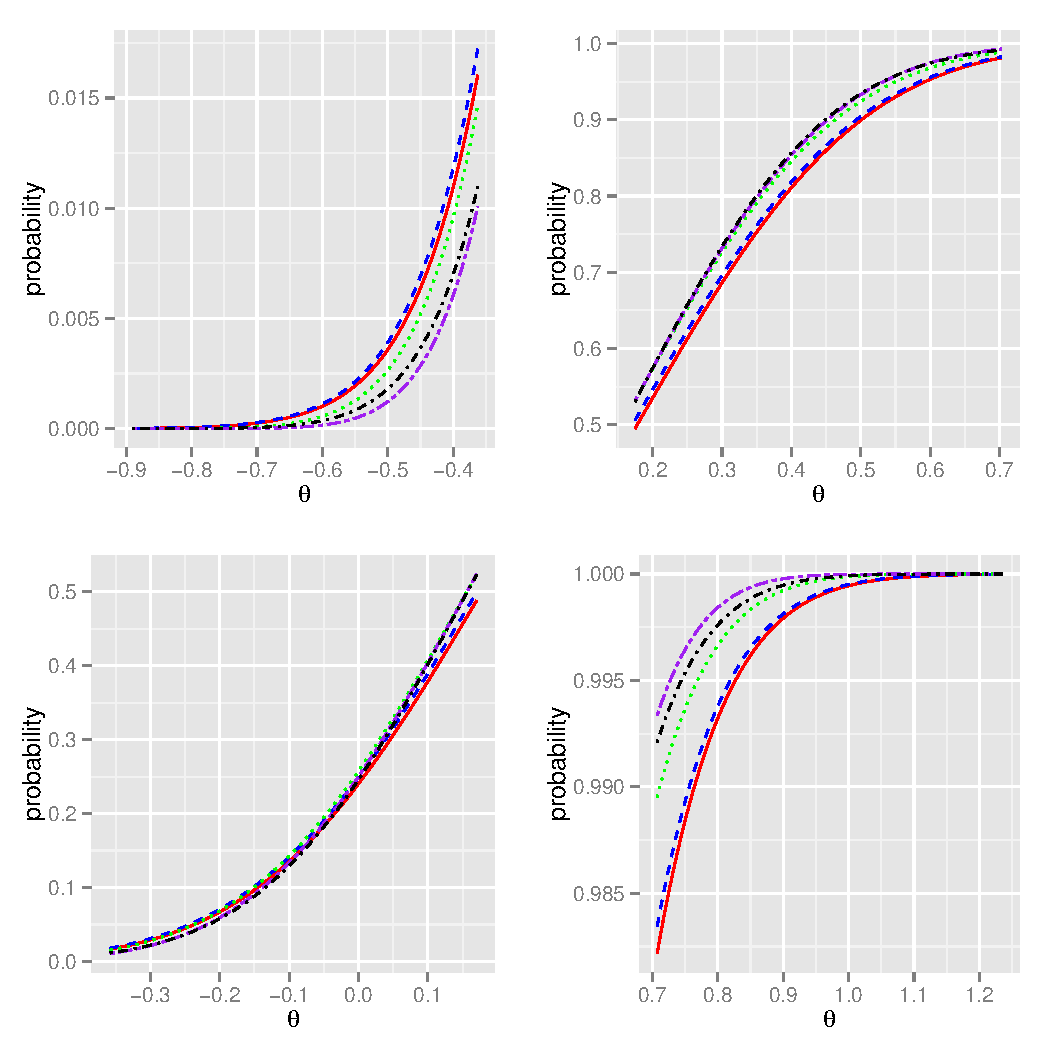
\includegraphics[scale=0.5]{n10bw.pdf}\protect\caption{Posterior cumulative distribution function when sample size is 10\label{fig:Posterior-CDF-n10}}
\end{center}

\end{figure}
\begin{figure}[H]

\begin{center}
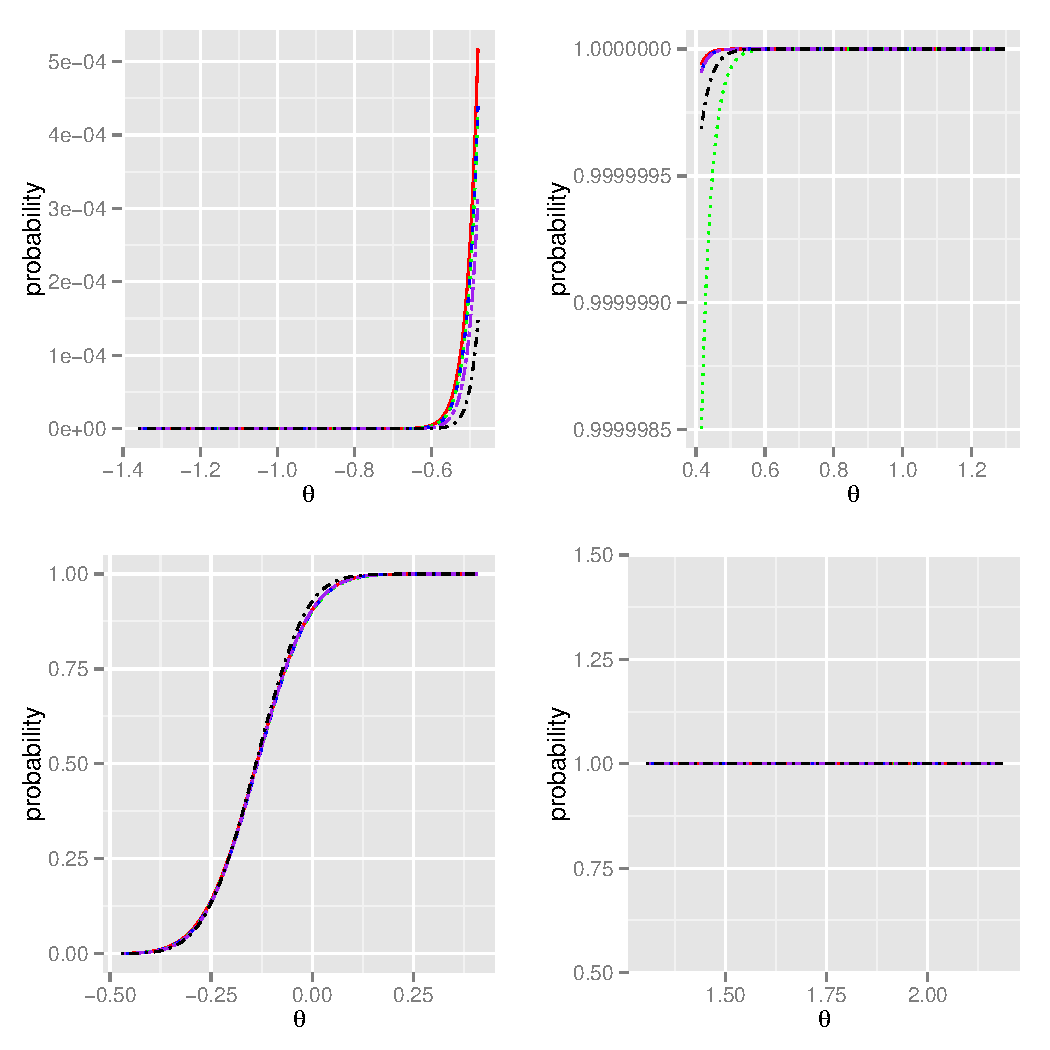
\includegraphics[scale=0.5]{n80bw.pdf}\protect\caption{Posterior cumulative distribution function when sample size is 80\label{fig:Posterior-CDF-n80}}
\end{center}

\end{figure}
 
\section{Discussion}
The paper provides an asymptotic expansion of the posterior based on an empirical likelihood subject to a linear constraint. The Bernstein --von Mises theorem and asymptotic expansions of the cumulative distribution function and the posterior mean are obtained as corollaries. Future work will include an extension to the multivariate case as well as expansions subject to multiple constraints. 



\chapter{Higher-Order Properties of Bayesian Empirical Likelihood: Multivariate
Case}


\section{Introduction}

Empirical likelihood, over the years, has become a very popular topic
of statistical research. The name was coined by Owen in his classic
1986 paper, although similar ideas are found even earlier in the works
of \citet{hartley1968new}, \citet{thomas1975confidence}, \citet{rubin1981bayesian}
and others. The main advantage of empirical likelihood is that is
involves fewer assumptions that a regular likelihood, and yet shares
the same asymptotic properties of the latter. 

Research in this area has primarily been frequentist with a long list
of important theoretical developments accompanied by a large number
of applications. To our knowledge, the first Bayesian work in this
general area appeared in the article of \citet{lazar2003bayesian}
followed by some related work in \citet{schennach2005bayesian,schennach2007point}
, the latter introducing the concept of ``exponentially tilted empirical
likelihood''. \citet{lazar2003bayesian} suggested using empirical
likelihood as a substitute for the usual likelihood and carry out
Bayesian analysis in the usual way. 

\citet{baggerly1998empirical} viewed empirical likelihood as a method
of assigning probabilities to a $n$-cell contingency table in order
to minimize a goodness-of-fit criterion. He selected Cressie-Read
power divergence statistics as one such criterion for construction
of confidence regions in a number of situations and pointed out also
how the usual empirical likelihood, exponentially tilted empirical
likelihood and others can be viewed as special cases of the Cressie-Read
criterion by appropriate choice of the the power parameter. This was
also discussed in \citet{owen2010empirical} who pointed our that
all members of the Cressie-Read family lead to ``empirical divergence
analogues of the empirical likelihood in which asymptotic $\chi^{2}$
calibration holds for the mean''.

The objective of this article is to provide an asymptotic expansion
of the posterior distribution based on empirical likelihood and its
variations under certain regularity conditions and a mean constraint.
The work is inspired by the work of \citet{fang2006empirical} who
provided a somewhat different expansion subject to a mean constraint.
Unlike \citet{fang2005expected,fang2006empirical}, our result is
based on the derivatives of the pseudo likelihood with respect to
the parameters of interest evaluated at the maximum EL estimator,
and a rigorous expansion is provided with particular attention in
handling the remainder terms. Moreover, we consider a general estimating
equation which includes the mean example of \citet{fang2006empirical}
as a special case. The need for different pseudo-likelihoods for statistical
inference is felt all the more in these days, especially for the analysis
of high-dimensional data, where the usual likelihood based analysis
is hard to perform, These alternative likelihoods are equally valuable
for approximate Bayesian computations (ABC), a topic which has only
recently surfaced in the statistics literature (see e.g. Comuet et
al. , 2008)%
\begin{comment}
paper not found or cornuet 2008
\end{comment}
.

Asymptotic expansion of the posterior based on a regular likelihood
was given earlier in \citet{johnson1970asymptotic}, and later in
\citet{ghosh1982expansions}. We follow their approach with many necessary
modifications in view of the fact that any meaningful prior needs
to have support in the nondecreasing compact set $H$. As a special
case of our result, we get the celebrated Bernstein von-Mises Theorem.
The latter was mentioned in \citet{lazar2003bayesian} for the special
case of empirical likelihood, but here we provide a rigorous  derivation
with the needed regularity conditions. 

Unlike in univariate case, where the posterior is centered at M-estimator,
which guarantees the consistency under mild regular conditions, in
multivariate case, the posterior is centralized at maximum generalized
empirical likelihood estimator. This concept is generalized from empirical
likelihood case which is fully explored in \citet{qin1994empirical}
to exponentially tilted empirical likelihood and even Cressie-Read
case. A similar concept has been developed in \citet{newey2004higher}
under the similar name. There is slight different between their definition
and ours in both intuition and mathematical definition, however, numerical
study shows the performance of these two are quite similar. Furthermore,
in order for the empirical likelihood sample moments to be finite,
we need more restrictive conditions to guarantee not only the consistency
of generalized empirical likelihood estimator, but also its law of
iterative logarithm. 

The organization of the remaining sections of this paper is as follows.
In Section 2 of this paper, we consider the basic settings of the
empirical likelihood, exponentially tilted empirical likelihood, and
finally the more general Cressie-Read divergence criterion. Section
3 contains some basic lemmas pertaining to these three formulations.
While both empirical and exponentially tilted empirical likelihood
are indeed limiting cases of the general Cressie-Read formulation,
for technical reasons as as well as for the sake of transparency,
we have presented some of these lemmas separately for these three
cases. Section 4 contains the main result, namely the asymptotic expansion
of the posterior and presents a unified derivation. Some simulation
results are presented in Section 5. Section 6 contains some concluding
remarks.


\section{Basic Settings}

Suppose $X_{1},\ldots,X_{n}$ are independent and identically distributed
random vectors satisfying $Eg\left(X_{1},\theta\right)=0$, where
$\theta\in\mathbb{R}^{p}$ and $g\left(x,\theta\right)=\left(g_{1}\left(x,\theta\right),g_{2}\left(x,\theta\right),\ldots,g_{r}\left(x,\theta\right)\right)\in\mathbb{R}^{r}$.
Like in \citet{qin1994empirical}, we focus on the situation $r>p$.
When $r\le p$, the posterior will still asymptotically center around
M-estimator, and all the arguments are the same as univariate case.
However, when $r>p$ , M-estimator may not even exist, we need further
generalization. In this context, \citet{owen1988empirical}, formulated
empirical likelihood as a nonparametric likelihood of the form $\prod_{i=1}^{n}w_{i}\left(\theta\right)$,
where $w_{i}$ is the probability mass assigned to $X_{i}\left(i=1,\ldots,n\right)$
satisfying the constraints 
\begin{equation}
\begin{cases}
w_{i}>0,\mathrm{for\: all\: i;}\\
\sum_{i=1}^{n}w_{i}=1;\\
\sum_{i=1}^{n}w_{i}g\left(X_{i},\theta\right)=0.
\end{cases}\label{eq:constraint-el}
\end{equation}
The target is to maximize $\prod_{i=1}^{n}w_{i}$ or equivalently
$\sum_{i=1}^{n}\log w_{i}$ with respect to $w_{1},\ldots,w_{n}$
subject to the constraints given in (\ref{eq:constraint-el}). Applying
the Lagrange multiplier method, the solution turns out to be 
\begin{equation}
\hat{w}_{i}^{\mathrm{EL}}\left(\theta\right)=\frac{1}{n\left[1+\nu^{T}g\left(X_{i},\theta\right)\right]},\; i=1,2,\ldots,n,\label{eq:sol-emp-lik}
\end{equation}
where $\nu\in\mathbb{R}^{r}$, the Lagrange multiplier satisfies 
\begin{equation}
\sum_{i=1}^{n}\frac{g\left(X_{i},\theta\right)}{1+\nu^{T}g\left(X_{i},\theta\right)}=0.\label{eq:lambda-eq}
\end{equation}


It may be noted that \citet{fang2005expected,fang2006empirical} $g\left(X_{i},\theta\right)=X_{i}-\theta$. 

Closely related to the empirical likelihood is the exponentially tilted
empirical likelihood where the objective is to maximize the Shannon
entropy $-\sum_{i=1}^{n}w_{i}\log w_{i}$ still subject to the constraints
in (\ref{eq:constraint-el}). The resulting solution is given by 
\begin{equation}
\hat{w}_{i}^{\mathrm{ET}}\left(\theta\right)=\frac{\exp\left(-\nu^{T}g\left(X_{i},\theta\right)\right)}{\sum_{j=1}^{n}\exp\left(-\nu^{T}g\left(X_{i},\theta\right)\right)},\label{eq:sol-weight-etel}
\end{equation}
where $\nu$, the Lagrange multiplier, satisfies 
\begin{equation}
\sum_{i=1}^{n}\exp\left(-\nu^{T}g\left(X_{i},\theta\right)\right)g\left(X_{i},\theta\right)=0.\label{eq:lag-mul-exp-tilt-el}
\end{equation}
The exponentially tilted empirical likelihood is related to Kullback-Leibler
divergence between two empirical distributions, one with weights $w_{i}$
assigned to the $n$ sample points, and the other with uniform weights
$1/n$ assigned to the sample points. 

The general Cressie-Read divergence criterion given by 
\[
\mathrm{CR}\left(\lambda\right)=\frac{2}{\lambda\left(\lambda+1\right)}\sum_{i=1}^{n}\left[\left(nw_{i}\right)^{-\lambda}-1\right].
\]
We focus on the cases $\lambda\ge0$ and $\lambda\le-1$, because
in these cases, $\mathrm{CR}\left(\lambda\right)$ is a convex function
of the $w_{i}\left(i=1,\ldots,n\right)$,hence the minimization
problem will produce a unique solution. The following lemma also shows
within this range, the resulting empirical weights behaviour more
like a likelihood. The limiting cases $\lambda\rightarrow0$ and $\lambda\rightarrow-1$
correspond to the usual empirical likelihood and the exponentially
tilted empirical likelihood as defined earlier. 

For convex $\mathrm{CR}\left(\lambda\right)$, its minimum will be
attained in the compact set $H_{n}$ determined by data. The Lagrange
multiplication method now gives the weights 
\begin{equation}
\hat{w}_{i}^{\mathrm{CR}}\left(\theta\right)=\frac{1}{n}\left(\mu+\nu^{T}g\left(X_{i},\theta\right)\right)^{-\frac{1}{\lambda+1}},\, i=1,2,\ldots,n,\label{eq:weight-cr-el}
\end{equation}
where $\mu\equiv\mu\left(\theta\right)$ and $\nu\equiv\nu\left(\theta\right)$
satisfy 
\begin{equation}
\begin{cases}
\sum_{i=1}^{n}\left(\mu+\nu^{T}Tg\left(X_{i},\theta\right)\right)^{-\frac{1}{\lambda+1}}=n,\\
\sum_{i=1}^{n}\left(\mu+\nu^{T}g\left(X_{i},\theta\right)\right)^{-\frac{1}{\lambda+1}}X_{i}=0.
\end{cases}\label{eq:lag-mul-cr-el}
\end{equation}


We now introduce the posterior based on an empirical likelihood. The
basic ideal was first introduced by \citet{lazar2003bayesian} with
bunch of numerical examples. The intuition relies on close relationship
between empirical likelihood and empirical distribution. \citet{owen2010empirical}
formulated 105 4 the two concepts under the same optimization framework,
that is, they shared the same objective function, but the former one
was solved under parametric constraints, while the latter was not.
Considering this similarity, we can use the empirical likelihood as
a valid distribution parametrized by inferential target. To concrete
this intuition in Bayesian philosophy, writing $\hat{w}_{i}\left(\theta\right)$
as generic notation for either $\hat{w}_{i}^{\mathrm{EL}}$, $\hat{w}_{i}^{\mathrm{ET}}$
or $\hat{w}_{i}^{\mathrm{CR}}$, $\pi$ with a prior probability density
function $\rho\left(\theta\right)$, with support in $H_{n}$, the
profile (pseudo) posterior is given by 
\begin{equation}
\pi\left(\theta\mid X_{1},X_{2},\ldots,X_{n}\right)=\frac{\prod_{i=1}^{n}\hat{w}_{i}\left(\theta\right)\rho\left(\theta\right)}{\int_{H_{n}}\prod_{i=1}^{n}\hat{w}_{i}\left(\theta\right)\rho\left(\theta\right)\diff\theta}.\label{eq:poster-el-expression}
\end{equation}


The main objective of this paper is to provide an asymptotic expansion
of $\pi\left(\theta\mid X_{1},X_{2},\ldots,X_{n}\right)$. This will
include in particular the Bernstein-von Mises theorem. Towards this
end, we develop a few necessary lemmas in the next section.


\section{Lemmas}

We first give an explanation of natural domain of $\theta$, under
empirical likelihood settings. In practice, some values of $\theta$
will result in an empty feasible set in constraints (\ref{eq:constraint-el}).
The which guarantees an non-empty feasible set, and thus a solution
of the optimization problem constitutes 120 natural domain of empirical
likelihood. One may questions whether the size of the natural domain
is large enough to contain the true value. The following lemma alleviates
this worry.
\begin{lem}
\label{lem:nondecreasing-compact-natural-domain}Assume $g\left(\cdot,\cdot\right)$
is a continuous vector value function, then the natural domain defined
by the constraints (\ref{eq:constraint-el}) is a compact set and
nondecreasing with respect to sample size $n$.\end{lem}
\begin{proof}
By the third constraint of (\ref{eq:constraint-el}), $\theta$ is
a continuous vector value function of $w_{1},w_{2},\ldots,w_{n}$,
but $w_{i}$ are defined on a simplex which is a compact set through
the first constraint of (\ref{eq:constraint-el}). We may recall that
continuous function maps compact sets to compact sets. Hence, $\theta$
is naturally defined on a compact set denoted by $H$.

If for any $j=1,2,\ldots,r$, $g_{j}\left(X_{i},\theta\right)$, $i=1,2,\ldots,n$,
are all non-positive or all non-negative, then the constraints (\ref{eq:constraint-el})
are violated and $H=\emptyset$. Hence ,
\begin{eqnarray*}
H & = & \left\{ \bigcup_{j=1}^{r}\left\{ \left[\bigcap_{i=1}^{n}\left(g_{j}\left(X_{i},\theta\right)\ge0\right)\right]\bigcup\left[\bigcap_{i=1}^{n}\left(g_{j}\left(X_{i},\theta\right)\le0\right)\right]\right\} \right\} ^{c}\\
 & = & \bigcap_{j=1}^{r}\left\{ \left[\bigcup_{i=1}^{n}\left(g_{j}\left(X_{i},\theta\right)\ge0\right)^{c}\right]\bigcap\left[\bigcup_{i=1}^{n}\left(g_{j}\left(X_{i},\theta\right)\le0\right)^{c}\right]\right\} .
\end{eqnarray*}
With $n$ increases, both $\bigcup_{i=1}^{n}\left(g_{j}\left(X_{i},\theta\right)\ge0\right)^{c}$
and $\bigcup_{i=1}^{n}\left(g_{j}\left(X_{i},\theta\right)\le0\right)^{c}$
will increase, so does their intersection $H$. 
\end{proof}
Although, intuitively we expect the empirical likelihood to behave
as the true likelihood, we need some theoretical support to show that
the former enjoys some of the basic properties of the latter. In particular,
we need to verify that $\nu$ and $\mu$ are smooth functions of $\theta$
and the (pseudo) Fisher Information based on the empirical likelihood
is positive. 

We first establish the positiveness of the Fisher information . We
consider the three cases separately to introduce more transparency
and continuity in our approach. 

Our first lemma shows that the Lagrange multipliers $\nu\left(\theta\right)$
and $\mu\left(\theta\right)$ are all smooth functions of $\theta$.
\begin{comment}
add condtions
\end{comment}

\begin{lem}
\label{lem:first-order-smooth-lagmul}For empirical likelihood, exponentially
tilted empirical likelihood and Cressie-Read with parameter$\left(\lambda\right)$,
the Lagrange multipliers $\nu\left(\theta\right)$ and $\mu\left(\theta\right)$
are smooth functions of $\theta.$\end{lem}
\begin{proof}
We first consider empirical likelihood and observe that, $\nu\left(\theta\right)$
is a implicit function of $\theta$ in view of (\ref{eq:lambda-eq})
. Further 
\[
\frac{\partial}{\partial\nu}\sum_{i=1}^{n}\frac{g\left(X_{i},\theta\right)}{1+\nu^{T}g\left(X_{i},\theta\right)}=-\sum_{i=1}^{n}\frac{g\left(X_{i},\theta\right)g^{T}\left(X_{i},\theta\right)}{\left(1+\nu^{T}g\left(X_{i},\theta\right)\right)^{2}},
\]
is negative definite, so that by the implicit function theorem, $\nu$
is differentiable in $\theta$. Moreover, differentiating both sides
of (\ref{eq:lambda-eq}) with respect to $\nu$, one gets
\begin{eqnarray*}
0 & = & \sum_{i=1}^{n}\frac{1}{1+\nu^{T}g\left(X_{i},\theta\right)}\frac{\partial g\left(X_{i},\theta\right)}{\partial\theta^{T}}\frac{\partial\theta}{\partial\nu}-\sum_{i=1}^{n}\frac{\nu^{T}g\left(X_{i},\theta\right)}{\left(1+\nu^{T}g\left(X_{i},\theta\right)\right)^{2}}\frac{\partial g\left(X_{i},\theta\right)}{\partial\theta^{T}}\frac{\partial\theta}{\partial\nu}\\
 &  & -\sum_{i=1}^{n}\frac{g\left(X_{i},\theta\right)g^{T}\left(X_{i},\theta\right)}{\left(1+\nu^{T}g\left(X_{i},\theta\right)\right)^{2}},
\end{eqnarray*}
which on simplification leads to 
\begin{equation}
\frac{\partial\theta}{\partial\nu}=-\left[\sum_{i=1}^{n}\frac{1}{\left(1+\nu^{T}g\left(X_{i},\theta\right)\right)^{2}}\frac{\partial g\left(X_{i},\theta\right)}{\partial\theta}\right]^{-1}\sum_{i=1}^{n}\frac{g\left(X_{i},\theta\right)g^{T}\left(X_{i},\theta\right)}{\left(1+\nu^{T}g\left(X_{i},\theta\right)\right)^{2}},\label{eq:decreasing-theta-to-nu}
\end{equation}


Next, for exponentially tilted empirical likelihood, in view of (\ref{eq:lag-mul-exp-tilt-el})
and the relation 
\begin{eqnarray*}
 &  & \frac{\partial}{\partial\nu}\left(\sum_{i=1}^{n}\exp\left(-\nu^{T}g\left(X_{i},\theta\right)\right)g\left(X_{i},\theta\right)\right)\\
 & = & -\sum_{i=1}^{n}\exp\left(-\nu^{T}g\left(X_{i},\theta\right)\right)g\left(X_{i},\theta\right)g^{T}\left(X_{i},\theta\right).
\end{eqnarray*}
Note that this matrix is negative definite. Once again, the implicit
function theorem guarantees the differentiability of $\nu$ in $\theta$.
Further, differentiating both sides of (\ref{eq:lag-mul-exp-tilt-el})
with respect to $\theta$, one gets 
\begin{equation}
\frac{\partial\nu}{\partial\theta}=\left(\sum_{i=1}^{n}\frac{g\left(X_{i},\theta\right)g^{T}\left(X_{i},\theta\right)}{\exp\left(-\nu^{T}g\left(X_{i},\theta\right)\right)}\right)^{-1}\left(\sum_{i=1}^{n}\frac{1-\nu^{T}g\left(X_{i},\theta\right)}{\exp\left(-\nu^{T}g\left(X_{i},\theta\right)\right)}\frac{\partial g\left(X_{i},\theta\right)}{\partial\theta}\right).\label{eq:first-deri-lag-mult-exp-tilted-el}
\end{equation}


A similar conclusion is achieved for $\nu\left(\theta\right)$ and
$\mu\left(\theta\right)$ defined in (\ref{eq:lag-mul-cr-el}) in
connection with CR$\left(\lambda\right)$. Specifically, defining
\[
\begin{cases}
F_{1}=\sum_{i=1}^{n}\left(\mu+\nu^{T}g\left(X_{i},\theta\right)\right)^{-\frac{1}{\lambda+1}}-n,\\
F_{2}=\sum_{i=1}^{n}\left(\mu+\nu^{T}g\left(X_{i},\theta\right)\right)^{-\frac{1}{\lambda+1}}g\left(X_{i},\theta\right),
\end{cases}
\]
it follows that,
\[
\frac{\partial\left(F_{1},F_{2}\right)}{\partial\left(\mu,\nu\right)}=-\frac{1}{\lambda+1}\left(\begin{array}{cc}
\sum_{i=1}^{n}q_{i} & \sum_{i=1}^{n}q_{i}g\left(X_{i},\theta\right)\\
\sum_{i=1}^{n}q_{i}g^{T}\left(X_{i},\theta\right) & \sum_{i=1}^{n}q_{i}g\left(X_{i},\theta\right)g^{T}\left(X_{i,},\theta\right)
\end{array}\right),
\]
 where $q_{i}=\left(\mu+\nu^{T}g\left(X_{i},\theta\right)\right)^{-\frac{1}{\lambda+1}-1}$
. Then the determinant of Jacobian is 
\begin{eqnarray*}
\det\frac{\partial\left(F_{1},F_{2}\right)}{\partial\left(\mu,\nu\right)} & = & \left(\frac{1}{\lambda+1}\right)^{2}\left(\sum_{i=1}^{n}q_{i}\sum_{i=1}^{n}q_{i}g\left(X_{i},\theta\right)g^{T}\left(X_{i},\theta\right)-\sum_{i=1}^{n}q_{i}g\left(X_{i},\theta\right)\sum_{i=1}^{n}q_{i}g^{T}\left(X_{i},\theta\right)\right)\\
 & = & \left(\frac{1}{\lambda+1}\right)^{2}\left(\sum_{i=1}^{n}q_{i}\right)^{2}\sum_{i=1}^{n}\frac{q_{i}}{\sum_{j=1}^{n}q_{j}}\left[g\left(X_{i},\theta\right)-\left(\sum_{i=1}^{n}\frac{q_{i}}{\sum_{j=1}^{n}q_{j}}g\left(X_{i},\theta\right)\right)\right]\\
 &  & \times\left[g\left(X_{i},\theta\right)-\left(\sum_{i=1}^{n}\frac{q_{i}}{\sum_{j=1}^{n}q_{j}}g\left(X_{i},\theta\right)\right)\right]^{T},
\end{eqnarray*}
which is positive definite. Again, by implicit function theorem, one
gets differentiability of $\mu\left(\theta\right)$ and $\nu\left(\theta\right)$with
respect to $\theta$, and 
\begin{eqnarray}
 &  & \left(\begin{array}{c}
\partial\mu/\partial\theta\\
\partial\nu/\partial\theta
\end{array}\right)\nonumber \\
 & = & \left(\frac{\partial\left(F_{1},F_{2}\right)}{\partial\left(\mu,\nu\right)}\right)^{-1}\left(\begin{array}{c}
\partial F_{1}/\partial\theta\\
\partial F_{2}/\partial\theta
\end{array}\right)\\
 & = & \left(-\frac{1}{\lambda+1}\right)\left(\lambda+1\right)^{2}\left[\sum_{i=1}^{n}q_{i}\sum_{i=1}^{n}q_{i}g\left(X_{i},\theta\right)g^{T}\left(X_{i},\theta\right)-\sum_{i=1}^{n}q_{i}g\left(X_{i},\theta\right)\sum_{i=1}^{n}q_{i}g^{T}\left(X_{i},\theta\right)\right]^{-1}\nonumber \\
 &  & \times\left(\begin{array}{cc}
\sum_{i=1}^{n}q_{i}g\left(X_{i},\theta\right)g^{T}\left(X_{i},\theta\right) & -\sum_{i=1}^{n}q_{i}g\left(X_{i},\theta\right)\\
-\sum_{i=1}^{n}q_{i}g^{T}\left(X_{i},\theta\right) & \sum_{i=1}^{n}q_{i}
\end{array}\right)\nonumber \\
 &  & \times\left(\begin{array}{c}
-\left(\lambda+1\right)^{-1}\sum_{i=1}^{n}q_{i}\nu^{T}\partial g\left(X_{i},\theta\right)/\partial\theta\\
-\left(\lambda+1\right)\sum_{i=1}^{n}q_{i}\nu^{T}g\left(X_{i},\theta\right)\partial g\left(X_{i},\theta\right)/\partial\theta+\sum_{i=1}^{n}\left(\mu+\nu^{T}g\left(X_{i},\theta\right)\right)^{\frac{1}{\lambda+1}}\partial g\left(X_{i},\theta\right)/\partial\theta
\end{array}\right)\label{eq:first-der-lag-mul-crel}
\end{eqnarray}

\end{proof}
The next result shows that all the derivatives of the Lagrange multipliers
$\nu\left(\theta\right)$ and $\mu\left(\theta\right)$ are smooth
functions of $\theta\in H$. We provide a unified proof for all three
cases where we utilize the previous lemma. 
\begin{assumption}
\label{assu:high-derive-cond}Assume for any $\left(k_{1},k_{2},\ldots,k_{p}\right)\in\mathbb{N}^{p}$,
satisfying $\sum_{i=1}^{p}k_{i}=k\le K+4$, the higher-order mixture
partial derivatives 
\[
\frac{\partial^{k}g\left(X,\theta\right)}{\partial\theta_{1}^{k_{1}}\partial\theta_{2}^{k_{2}}\cdots\partial\theta_{p}^{k_{p}}},
\]
exists and continuous in $\theta$, almost surely in $X$.\end{assumption}
\begin{lem}
\label{lem:mul-el-smooth-lagrange-mul-1}Under the Assumption \ref{assu:high-derive-cond},
all partial derivatives of $\nu\left(\theta\right)$ and $\mu\left(\theta\right)$
are smooth functions of $\theta$ for $\theta\in H$.\end{lem}
\begin{proof}
The result is proved by induction. We have see already in Lemma \ref{lem:first-order-smooth-lagmul},
the gradient $\nabla\nu\left(\theta\right)$ and $\nabla\mu\left(\theta\right)$
are smooth functions of $\theta$. Suppose the result holds for all
$k$th partial derivatives of $\nu\left(\theta\right)$ and $\mu\left(\theta\right)$
for $k\le K$. The writing 
\[
\nabla^{k}\nu\left(\theta\right)=h_{k}\left(\nu\left(\theta\right),\theta\right),1\le k\le K,
\]
 
\[
\nabla^{k+1}\nu\left(\theta\right)=\frac{\partial h_{k}}{\partial\nu^{T}}\nabla\nu+\frac{\partial h_{k}}{\partial\theta}
\]
which is also a smooth function of $\theta$ by the induction hypothesis
and Lemma 1. A similar proof works for $\mu\left(\theta\right)$.
\end{proof}

\section{Maximum Generalized Empirical Likelihood Estimator}

One important justification of maximum likelihood estimator is the
good performance substantiated by large sample theory, such as consistency
and asymptotic normality. It can be shown the above theoretical results
can be seamlessly transplanted onto the estimator resulted from maximum
empirical weights. \citet{qin1994empirical} already pointed out the
validity to use empirical likelihood to define maximum empirical likelihood
estimator. We extend the same idea into more general Cressie-Read
family. 
\begin{defn}[Maximum Generalized Empirical Likelihood Estimator]
\label{def:gmele}Let $\hat{w}_{i}\left(\theta\right)$ be the empirical
weights on sample $X_{1},X_{2},\ldots,X_{n}$, generating from empirical
likelihood, exponentially tilted empirical likelihood or Cressie-Read
family. Then 
\[
\tilde{\theta}=\argmin_{\theta\in H}-\sum_{i=1}^{n}\log\hat{w}_{i}\left(\theta\right),
\]
called  maximum generalized empirical likelihood estimator.
\end{defn}
Lemma \ref{lem:mul-el-smooth-lagrange-mul-1} establishes the continuity
of empirical likelihood and Lemma \ref{lem:nondecreasing-compact-natural-domain}
reveals the compactness of $H$, then these results guarantee the
existence of $\tilde{\theta}$. So this concept is well-defined. One
advantage of this estimator over the traditional M-estimator is that
it can always produce a good quality estimator even when traditional
one has no solution. Before exploring the asymptotic properties of
this new estimator, we derive an equivalent formulation of  maximum
generalized empirical likelihood estimator, which may be more appropriate
for numerical computation and theoretical derivation. 

First, we define $\Psi$ functions under the three cases. In empirical
likelihood case, let 
\begin{eqnarray*}
\Psi_{1}\left(x\mid\theta,\nu\right) & = & \frac{g\left(x,\theta\right)}{1+\nu^{T}g\left(x,\theta\right)},\\
\Psi_{2}\left(x\mid\theta,\nu\right) & = & \frac{1}{1+\nu^{T}g\left(x,\theta\right)}\nu^{T}\frac{\partial g\left(x,\theta\right)}{\partial\theta}.
\end{eqnarray*}
Let $\Psi^{\mathrm{EL}}\left(x\mid\theta,\nu\right)=\left(\Psi_{1},\Psi_{2}\right)^{T}$.
In exponentially tilted empirical likelihood, let 
\begin{eqnarray*}
\Psi_{1}\left(x\mid\theta,\nu,\mu,\lambda_{1},\lambda_{2}\right) & = & \nu^{T}\frac{\partial g\left(x,\theta\right)}{\partial\theta}-\lambda_{1}\exp\left(-\mu-\nu^{T}g\left(x,\theta\right)\right)\nu^{T}\frac{\partial g\left(x,\theta\right)}{\partial\theta}\\
 &  & -\exp\left(-\mu-\nu^{T}g\left(x,\theta\right)\right)\nu^{T}\frac{\partial g\left(x,\theta\right)}{\partial\theta}\lambda_{2}^{T}g\left(x,\theta\right)+\exp\left(-\mu-\nu^{T}g\left(x,\theta\right)\right)\lambda_{2}^{T}\frac{\partial g\left(x,\theta\right)}{\partial\theta},\\
\Psi_{2}\left(x\mid\theta,\nu,\mu,\lambda_{1},\lambda_{2}\right) & = & g\left(x,\theta\right)-\lambda_{1}\exp\left(-\mu-\nu^{T}g\left(x,\theta\right)\right)g\left(x,\theta\right)-\exp\left(-\mu-\nu^{T}g\left(x,\theta\right)\right)g\left(x,\theta\right)\lambda_{2}^{T}g\left(x,\theta\right),\\
\Psi_{3}\left(x\mid\theta,\nu,\mu,\lambda_{1},\lambda_{2}\right) & = & 1-\lambda_{1}\exp\left(-\mu-\nu^{T}g\left(x,\theta\right)\right)-\exp\left(-\mu-\nu^{T}g\left(x,\theta\right)\right)\lambda_{2}^{T}g\left(x,\theta\right),\\
\Psi_{4}\left(x\mid\theta,\nu,\mu,\lambda_{1},\lambda_{2}\right) & = & \exp\left(-\mu-\nu^{T}g\left(x,\theta\right)\right)-\frac{e}{n},\\
\Psi_{4}\left(x\mid\theta,\nu,\mu,\lambda_{1},\lambda_{2}\right) & = & \exp\left(-\mu-\nu^{T}g\left(x,\theta\right)\right)g\left(x,\theta\right),
\end{eqnarray*}
where $\lambda_{1}$ and $\lambda_{2}$ are new Lagrange multipliers
which we will define in later lemma. Let $\Psi^{\mathrm{ET}}\left(x\mid\theta,\nu,\mu,\lambda_{1},\lambda_{2}\right)=\left(\Psi_{1},\ldots,\Psi_{5}\right)^{T}.$
In Cressie-Read case, let 
\begin{eqnarray*}
\Psi_{1}\left(x\mid\theta,\nu,\mu,\lambda_{1},\lambda_{2}\right) & = & \frac{1}{\lambda+1}\Bigg[\frac{\nu^{T}\partial g\left(x,\theta\right)/\partial\theta}{\mu+\nu^{T}g\left(x,\theta\right)}-\lambda_{1}\frac{\nu^{T}\partial g\left(x,\theta\right)/\partial\theta}{\left(\mu+\nu^{T}g\left(x,\theta\right)\right)^{1+1/\left(\lambda+1\right)}}\\
 &  & -\frac{\left(\nu^{T}\partial g\left(x,\theta\right)/\partial\theta\right)\left(\lambda_{2}^{T}g\left(x,\theta\right)\right)}{\left(\mu+\nu^{T}g\left(x,\theta\right)\right)^{1+1/\left(\lambda+1\right)}}+\frac{\lambda_{2}^{T}\partial g\left(x,\theta\right)/\partial\theta}{\left(\mu+\nu^{T}g\left(x,\theta\right)\right)^{1+1/\left(\lambda+1\right)}}\Bigg],\\
\Psi_{2}\left(x\mid\theta,\nu,\mu,\lambda_{1},\lambda_{2}\right) & = & \frac{1}{\lambda+1}\left[\frac{g\left(x,\theta\right)}{\mu+\nu^{T}g\left(x,\theta\right)}-\lambda_{1}\frac{g\left(x,\theta\right)}{\left(\mu+\nu^{T}g\left(x,\theta\right)\right)^{1+1/\left(\lambda+1\right)}}-\frac{g\left(x,\theta\right)\left(\lambda_{2}^{T}g\left(x,\theta\right)\right)}{\left(\mu+\nu^{T}g\left(x,\theta\right)\right)^{1+1/\left(\lambda+1\right)}}\right],\\
\Psi_{3}\left(x\mid\theta,\nu,\mu,\lambda_{1},\lambda_{2}\right) & = & \frac{1}{\lambda+1}\Bigg[\frac{1}{\mu+\nu^{T}g\left(x,\theta\right)}-\lambda_{1}\left(\mu+\nu^{T}g\left(x,\theta\right)\right)^{-1-1/\left(\lambda+1\right)}\\
 &  & -\left(\mu+\nu^{T}g\left(x,\theta\right)\right)^{-1-1/\left(\lambda+1\right)}\lambda_{2}^{T}g\left(x,\theta\right)\Bigg],\\
\Psi_{4}\left(x\mid\theta,\nu,\mu,\lambda_{1},\lambda_{2}\right) & = & \left(\mu+\nu^{T}g\left(x,\theta\right)\right)^{-1/\left(\lambda+1\right)}-1,\\
\Psi_{5}\left(x\mid\theta,\nu,\mu,\lambda_{1},\lambda_{2}\right) & = & \left(\mu+\nu^{T}g\left(x,\theta\right)\right)^{-1/\left(\lambda+1\right)}g\left(x,\theta\right).
\end{eqnarray*}
Let $\Psi^{\mathrm{CR}}\left(x\mid\theta,\nu,\mu,\lambda_{1},\lambda_{2}\right)=\left(\Psi_{1},\ldots,\Psi_{5}\right)^{T}$.
Use above definitions, we elicit the following lemma.
\begin{lem}
\label{lem:extend-m-estimator}The  maximum generalized empirical
likelihood estimator is the solution of $n^{-1}\sum_{i=1}^{n}\Psi\left(X_{i}\mid\theta,\nu,\mu,\lambda_{1},\lambda_{2}\right)=0$.
If we denote the solution as $\left(\theta^{*},\nu^{*},\mu^{*},\lambda_{1}^{*},\lambda_{2}^{*}\right)$,
then $\tilde{\theta}=\theta^{*}$, $\nu\left(\tilde{\theta}\right)=\nu^{*}$
and $\mu\left(\tilde{\theta}\right)=\mu^{*}$.\end{lem}
\begin{proof}
For explicit, we state the proof separately under the three kinds
of empirical likelihoods. 

First in empirical likelihood. The relationship between $\theta$
and $\nu$ are restricted by equation constraint (\ref{eq:lambda-eq}).
By the Definition \ref{def:gmele}, the maximum generalized empirical
likelihood estimator can also be the solution of 
\[
\max_{\theta,\nu}l\left(\theta\right)=-\frac{1}{n}\sum_{i=1}^{n}\log\left(1+\nu^{T}g\left(X_{i},\theta\right)\right),
\]
subject to, 
\[
\sum_{i=1}^{n}\frac{g\left(X_{i},\theta\right)}{1+\nu^{T}g\left(X_{i},\theta\right)}=0.
\]
Directly calculation shows 
\[
\frac{\partial l\left(\theta\right)}{\partial\nu}=\frac{1}{n}\sum_{i=1}^{n}\frac{g\left(X_{i},\theta\right)}{1+\nu^{T}g\left(X_{i},\theta\right)}=\frac{1}{n}\sum_{i=1}^{n}\Psi_{1}\left(X_{i}\mid\theta,\nu\right).
\]
So the solution of unconstrained problem automatically satisfies the
constraint (\ref{eq:lambda-eq}). Moreover, 
\[
\frac{\partial l\left(\theta\right)}{\partial\theta}=\frac{1}{n}\sum_{i=1}^{n}\Psi_{2}\left(X_{i}\mid\theta,\nu\right).
\]
So the equation system $n^{-1}\sum_{i=1}^{n}\Psi\left(X_{i}\mid\theta,\nu\right)=0$
is the first order necessary condition of the optimization problem,
hence the lemma holds in empirical likelihood case.

Next, we consider exponentially tilted empirical likelihood. Reviewing
the Lagrange method to get the empirical weights (\ref{eq:sol-weight-etel}),
we find 
\[
\hat{w}_{i}\left(\theta\right)=\exp\left(-1-\mu-\nu^{T}g\left(X_{i},\theta\right)\right),
\]
where $\mu$ and $\nu$ satisfy 
\begin{eqnarray*}
\sum_{i=1}^{n}\exp\left(-1-\mu-\nu^{T}g\left(X_{i},\theta\right)\right) & = & 1,\\
\sum_{i=1}^{n}\exp\left(-1-\mu-\nu^{T}g\left(X_{i},\theta\right)\right)g\left(X_{i},\theta\right) & = & 0.
\end{eqnarray*}
 Hence, the optimization problem in Definition \ref{def:gmele} shares
the same maximum as the problem 
\[
\max_{\theta,\nu,\mu}l\left(\theta\right)=\frac{1}{n}\sum_{i=1}^{n}\left(-1-\mu-\nu^{T}g\left(X_{i},\theta\right)\right),
\]
subject to 
\begin{eqnarray*}
\sum_{i=1}^{n}\exp\left(-1-\mu-\nu^{T}g\left(X_{i},\theta\right)\right) & = & 1,\\
\sum_{i=1}^{n}\exp\left(-1-\mu-\nu^{T}g\left(X_{i},\theta\right)\right)g\left(X_{i},\theta\right) & = & 0.
\end{eqnarray*}
Unlike in empirical likelihood case, here we do not have any shortcut.
The Lagrange multiplier method is the only choice. The Lagrangian
can be written as 
\begin{eqnarray*}
L\left(\theta,\nu,\mu,\lambda_{1},\lambda_{2}\right) & = & \frac{1}{n}\sum_{i=1}^{n}\left(-1-\mu-\nu^{T}g\left(X_{i},\theta\right)\right)+\lambda_{1}\left(\sum_{i=1}^{n}\exp\left(-\mu-\nu^{T}g\left(X_{i},\theta\right)\right)-e\right)\\
 &  & +\lambda_{2}^{T}\left(\sum_{i=1}^{n}\exp\left(-1-\mu-\nu^{T}g\left(X_{i},\theta\right)\right)g\left(X_{i},\theta\right)\right).
\end{eqnarray*}
Calculation shows $\nabla L=n^{-1}\sum_{i=1}^{n}\Psi\left(X_{i}\mid\theta,\nu,\mu,\lambda_{1},\lambda_{2}\right)$.
Hence, the same argument supporting empirical likelihood case validate
the lemma in exponentially tilted empirical likelihood case.

The Cressie-Read case can follow exactly the same procedure in exponentially
tilted empirical likelihood case.
\end{proof}
This lemma offer a better numerical scheme to get the maximum generalized
empirical likelihood estimator than the original definition. In original
definition, for each iteration of $\theta$, one need to solve nonlinear
equations to get Lagrange multiplier $\nu$, which will introduce
another iteration. By using the first order condition as in this lemma,
we can use usual nonlinear equation solver to get the result in a
single layer iteration. The benefit of Lemma \ref{lem:extend-m-estimator}
also enlighten a quick solution on asymptotic properties of maximum
generalized empirical likelihood estimator. Indeed, it is trivial
to see, 
\begin{eqnarray*}
E\Psi^{\mathrm{EL}}\left(X\mid\theta_{0},0\right) & = & 0,\\
E\Psi^{\mathrm{ET}}\left(X\mid\theta_{0},0,-1,0\right) & = & 0,\\
E\Psi^{\mathrm{CR}}\left(X\mid\theta_{0},0,1,0,1\right) & = & 0.
\end{eqnarray*}
Hence, maximum generalized empirical likelihood estimator can also
be interpreted as an ordinary M-estimator defined by $\Psi$ function.
The consistency and asymptotic normality can be easily extracted from
ordinary M-estimator theory. However, in order to expand the posterior
around maximum generalized empirical likelihood estimator, we need
a slight stronger asymptotic property called law of iterative logarithm.
Particularly, the consistency requires the following condition.
\begin{assumption}
\label{assu:consistency-m-est}%
\begin{comment}
need to be specified
\end{comment}
add later consistency
\end{assumption}
The assumptions we need come from \citet{he1995law}. We state them
as follows.
\begin{assumption}
\label{assu:lil-m-est}Let $\eta=\left(\theta,\nu,\mu,\lambda_{1},\lambda_{2}\right)$.
Let $\psi\left(\eta\right)=E\Psi\left(X\mid\eta\right)$, $u\left(x,\eta,d\right)=\sup_{\left|\tau-\eta\right|\le d}\left|\Psi\left(x\mid\tau\right)-\Psi\left(x\mid\eta\right)\right|$,
where $\left|\cdot\right|$ takes sup-norm $\left|\eta\right|=\max_{1\le j\le p}\left|\eta_{j}\right|$.
Let $\eta_{n}$ satisfy 
\[
\frac{1}{\sqrt{n\log\log n}}\sum_{i=1}^{n}\Psi\left(X_{i}\mid\eta_{n}\right)\rightarrow0,\ascv.
\]
 The following conditions guarantee law of iterative logarithm.\end{assumption}
\begin{enumerate}
\item For each fixed $\eta\in H$, $\Psi\left(x\mid\eta\right)$ is square
integrable in $\eta$ and separable in sense of Doob: there is zero
measure set $N$ and a countable subset of $H'\subset H$, such that
for every open set $U\subset H$, and every closed interval $A$,
the sets $\left\{ x:\Psi\left(x\mid\eta\right)\in A,\:\forall\eta\in U\right\} $
and $\left\{ x:\Psi\left(x\mid\eta\right)\in A,\:\forall\eta\in U\cap H'\right\} $
differ by a subset of $N$.

\begin{enumerate}
\item There is a $\eta_{0}\in H$, such that $\psi\left(\eta_{0}\right)=0$,
and $\psi$ has a non-singular derivative at $\eta_{0}$.
\item There exist positive numbers $a,\: b,\: c,\: d,\:\alpha,\:\beta$,
and $d_{0}$ such that $\alpha\ge\beta>2$, and 

\begin{enumerate}
\item $\left|\psi\left(\eta\right)\right|\ge a\left|\eta-\eta_{0}\right|$,
for $\left|\eta-\eta_{0}\right|\le d_{0}$,
\item $Eu\left(x,\eta,d\right)\le bd$, for $\left|\eta-\eta_{0}\right|+d\le d_{0}$,
\item $Eu^{\alpha}\left(x,\eta,d\right)\le cd^{\beta}$, for $\left|\eta-\eta_{0}\right|+d\le d_{0}$.
\end{enumerate}
\item $\left|\eta_{n}-\eta_{0}\right|\le d_{0}$ almost surely as $n$ goes
infinity.
\end{enumerate}
\end{enumerate}
Actually, the second condition is merely requiring we have a theoretical
target, and the fourth condition is automatically satisfied if we
have consistency. Immediately by the theorem in \citet{he1995law},
we get the law of iterative logarithm for both maximum generalized
empirical likelihood estimator and the Lagrange multipliers. Now we
are ready to state another lemma to tie the empirical likelihood weights
and likelihood together with following condition on the unknown distribution.
\begin{assumption}
\label{assu:finite-theoretic-moment} Let $\left(k_{j1},k_{j2},\ldots,k_{jp}\right)\in\mathbb{N}^{p}$,
and $\sum_{i=1}^{p}k_{ji}=k_{j}\le K+4$, $j=1,\ldots,l$, then 
\[
E\left(\prod_{j=1}^{l}\frac{\partial^{k_{l}}g\left(X,\theta_{0}\right)}{\partial\theta_{1}^{k_{l1}}\partial\theta_{2}^{k_{l2}}\cdots\partial\theta_{p}^{k_{lp}}}\right),
\]
exists and finite.\end{assumption}
\begin{lem}
\label{lem:finite-empirical weight moment}Let $\omega_{i}\left(\theta\right)$
be the unnormalized empirical weights from empirical likelihood, that
is $\omega_{i}\left(\theta\right)=n\hat{w}_{i}\left(\theta\right)$
in empirical likelihood or Cressie-Read case, and $\omega_{i}\left(\theta\right)=\exp\left(-\nu\left(\theta\right)g\left(X_{i},\theta\right)\right)$
in exponentially tilted empirical likelihood. Use the same notation
in Assumption \ref{assu:high-derive-cond}. Under the Assumption \ref{assu:high-derive-cond},
\ref{assu:consistency-m-est}, \ref{assu:lil-m-est} and \ref{assu:finite-theoretic-moment},
then for any $k\le K+4$, any number $s\in\mathbb{R}$, 
\[
\lim_{n\rightarrow\infty}\frac{1}{n}\sum_{i=1}^{n}\omega_{i}\left(\tilde{\theta}\right)^{s}\prod_{j=1}^{l}\frac{\partial^{k_{l}}g\left(X,\theta_{0}\right)}{\partial\theta_{1}^{k_{l1}}\partial\theta_{2}^{k_{l2}}\cdots\partial\theta_{p}^{k_{lp}}}=E\left(\prod_{j=1}^{l}\frac{\partial^{k_{l}}g\left(X,\theta_{0}\right)}{\partial\theta_{1}^{k_{l1}}\partial\theta_{2}^{k_{l2}}\cdots\partial\theta_{p}^{k_{lp}}}\right)\ascv.
\]
\end{lem}
\begin{proof}
By the similar proof in %
\begin{comment}
add detail lemma number
\end{comment}
{} \citet{owen2010empirical}, we have 
\[
\lim_{n\rightarrow\infty}\max_{1\le i\le n}n^{-1/3}g\left(X_{i},\theta_{0}\right)=0\ascv.
\]
By law of iterative logarithm on Lagrange multiplier $\nu$, there
exists some constant $C_{1}$ 
\[
\varlimsup_{n\rightarrow\infty}\frac{\sqrt{n}\nu\left(\tilde{\theta}\right)}{\sqrt{2\log\log n}}=C_{1}\ascv.
\]
Hence 
\[
\varlimsup_{n\rightarrow\infty}\nu^{T}\left(\tilde{\theta}\right)\max_{1\le i\le n}g\left(X_{i},\tilde{\theta}\right)=o\left(\sqrt{\frac{2\log\log n}{n}}\times n^{1/3}\right)=o\left(\frac{\sqrt{2\log\log n}}{n^{1/6}}\right)=0.
\]
So $\nu^{T}\left(\tilde{\theta}\right)g\left(X_{i},\tilde{\theta}\right)$
are uniformly going to zero. Hence $\omega_{i}\left(\tilde{\theta}\right)$
are uniformly going to 1 and the lemma holds.
\end{proof}
This lemma supports consistency of empirical sample moment to true
moment and further justifies the intuition to use empirical likelihood
as a valid likelihood. 

\citet{newey2004higher} proposes a similar estimator replacing the
objective function in Definition \ref{def:gmele} with divergence
measure when one calculates empirical weights. Their definition coincides
with us when the divergence measure is empirical likelihood. Although,
their starting point is generalized method of moment estimator and
the intuition is slight different from us, the simulation hardly differs
the performance. In Table \ref{tab:mgele-mde}, we present the simulation
result. 
\begin{table}
% latex table generated in R 3.1.0 by xtable 1.7-3 package % Fri Apr 03 14:30:16 2015
%\begin{table}[ht]
\centering
\begin{tabular}{rrrrr}
  \hline
 & MGELE ETEL & MDE ETEL & MGELE CR & MDE CR \\ 
  \hline
N=20 & 0.1394 & 0.1320 & 0.2130 & 0.1408 \\
   N=50 & 0.0759 & 0.0759 & 0.1867 & 0.0766 \\
   N=100 & 0.0536 & 0.0536 & 0.2099 & 0.0539 \\
   N=200 & 0.0392 & 0.0401 & 0.2214 & 0.0396 \\
   N=500 & 0.0274 & 0.0298 & 0.1824 & 0.0274 \\
    \hline
\end{tabular}
%\end{table}\protect\caption{\label{tab:mgele-mde}Compare Performance MGELE and MDE}
\end{table}



\section{old stuff have not been modified}
\begin{lem}
\label{lem:bell-shape-el} %
\begin{comment}
need condition 
\end{comment}
$\diff^{2}\tilde{l}\left(\tilde{\theta}\right)/\diff\theta^{2}<0$
where $\tilde{l}\left(\theta\right)=n^{-1}\sum_{i=1}^{n}\log\hat{w}_{i}\left(\theta\right)$
where $\hat{w}_{i}$ is either $\hat{w}_{i}^{\mathrm{EL}}$, $\hat{w}_{i}^{\mathrm{ET}}$
or $\hat{w}_{i}^{\mathrm{CR}}$ $\left(i=1,2,\ldots,n\right)$.\end{lem}
\begin{proof}
We begin with $\tilde{l}\left(\theta\right)=n^{-1}\sum_{i=1}^{n}\log\hat{w}_{i}^{\mathrm{EL}}\left(\theta\right)=-\sum_{i=1}^{n}\log\left[1+\nu\left(X_{i}-\theta\right)\right]-\log n$.
Hence by (\ref{eq:sol-emp-lik}) and (\ref{eq:lambda-eq}), 
\[
\frac{\diff\tilde{l}\left(\theta\right)}{\diff\theta}=\frac{1}{n}\nu\sum_{i=1}^{n}\frac{1}{1+\nu g\left(X_{i}\theta\right)}\frac{\diff g\left(X_{i},\theta\right)}{\diff\theta}-\frac{1}{n}\sum_{i=1}^{n}\frac{g\left(X_{i}\theta\right)}{1+\nu g\left(X_{i}\theta\right)}\frac{\diff\nu}{\diff\theta}=\frac{1}{n}\nu\left(\theta\right)\sum_{i=1}^{n}\frac{1}{1+\nu g\left(X_{i}\theta\right)}\frac{\diff g\left(X_{i},\theta\right)}{\diff\theta}.
\]


Thus 
\[
\left.\frac{\diff^{2}\tilde{l}\left(\theta\right)}{\diff\theta^{2}}\right|_{\theta=\tilde{\theta}}=-\frac{\left(\sum_{i=1}^{n}\diff g\left(X_{i},\tilde{\theta}\right)/\diff\theta\right)^{2}}{n\sum_{i=1}^{n}g\left(X_{i},\tilde{\theta}\right)^{2}}<0.
\]


Next we consider $\tilde{l}\left(\theta\right)=n^{-1}\sum_{i=1}^{n}\log\hat{w}_{i}^{\mathrm{ET}}\left(\theta\right)=-\left(\nu n^{-1}\sum_{i=1}^{n}g\left(X_{i},\theta\right)+\log\sum_{i=1}^{n}\exp\left(-\nu g\left(X_{i},\theta\right)\right)\right)$.
Then 
\begin{eqnarray*}
\frac{\diff\tilde{l}\left(\theta\right)}{\diff\theta} & = & -\frac{\diff\nu}{\diff\theta}\frac{1}{n}\sum_{i=1}^{n}g\left(X_{i},\theta\right)\\
 &  & +\frac{\sum_{i=1}^{n}\exp\left(-\nu g\left(X_{i},\theta\right)\right)\left(\diff\nu/\diff\theta g\left(X_{i},\theta\right)+\nu\diff g\left(X_{i},\theta\right)/\diff\theta\right)}{\sum_{i=1}^{n}\exp\left(-\nu g\left(X_{i},\theta\right)\right)}\\
 & = & -\frac{\diff\nu}{\diff\theta}\frac{1}{n}\sum_{i=1}^{n}g\left(X_{i},\theta\right)+\nu\frac{\sum_{i=1}^{n}\exp\left(-\nu g\left(X_{i},\theta\right)\right)\diff g\left(X_{i},\theta\right)/\diff\theta}{\sum_{i=1}^{n}\exp\left(-\nu g\left(X_{i},\theta\right)\right)}\\
 &  & -\nu n^{-1}\sum_{i=1}^{n}\frac{\diff g\left(X_{i},\theta\right)}{\diff\theta}.
\end{eqnarray*}
Thus 
\[
\left.\frac{\diff^{2}\tilde{l}\left(\theta\right)}{\diff\theta^{2}}\right|_{\theta=\tilde{\theta}}=-\frac{\diff\nu}{\diff\theta}\frac{1}{n}\sum_{i=1}^{n}\frac{\diff g\left(X_{i},\tilde{\theta}\right)}{\diff\theta}=-\frac{\left(\sum_{i=1}^{n}\diff g\left(X_{i},\tilde{\theta}\right)/\diff\theta\right)^{2}}{n\sum_{i=1}^{n}g\left(X_{i},\tilde{\theta}\right)^{2}}<0.
\]


Finally, for CR, $\tilde{l}\left(\theta\right)=n^{-1}\sum_{i=1}^{n}\log\hat{w}_{i}^{\mathrm{CR}}\left(\theta\right)=-\left[n\left(\lambda+1\right)\right]^{-1}\sum_{i=1}^{n}\log\left(\mu+\nu g\left(X_{i},\theta\right)\right)$.
Then by (\ref{eq:first-der-lag-mul-crel}), 
\[
\frac{\diff\tilde{l}\left(\theta\right)}{\diff\theta}=.
\]
\begin{comment}
need to compute the first and second order derivative
\end{comment}
Thus 
\[
\left.\frac{\diff^{2}\tilde{l}\left(\theta\right)}{\diff\theta^{2}}\right|_{\theta=\overline{X}}=-\frac{\left(\sum_{i=1}^{n}\diff g\left(X_{i},\tilde{\theta}\right)/\diff\theta\right)^{2}}{n\sum_{i=1}^{n}g\left(X_{i},\tilde{\theta}\right)^{2}}.
\]

\end{proof}
Let $b=\left[\left(n^{-1}\sum_{i=1}^{n}\diff g\left(X_{i},\tilde{\theta}\right)/\diff\theta\right)^{2}/\left(n^{-1}\sum_{i=1}^{n}g\left(X_{i},\tilde{\theta}\right)^{2}\right)\right]^{-1/2}$.
Now we prove the main result in the next section.


\section{Assumptions}
\begin{enumerate}
\item \label{enu:multv-diff-full-rank}In multivariate empirical likelihood
settings, matrix $Z$ has full column rank with probability 1. %
\begin{comment}
brief discussion the stat meaning of assumption
\end{comment}

\item \label{enu:finite-moment-sample}$E\prod_{s=1}^{K}\left(X_{ij_{s}}-\theta_{j_{s},0}\right),\left(j_{1},j_{2},\ldots,j_{K}\right)\subset\left\{ 1,2,\ldots,K\right\} $,
where $\theta_{0}$ is the true expectation of $X$, exists and finite.
\begin{comment}
need a math induction lemma for finiteness of constant, need to be
more specified
\end{comment}
\begin{comment}
need a uniform bounded
\end{comment}

\item \label{enu:smooth-piror}The support of prior contains $H_{n}$, and
$\rho\left(\theta\right)\in C^{K}$. 
\item \label{enu:pd-sample-var}With probability 1 in $P_{X}^{n}$, $n^{-1}\sum_{i=1}^{n}\left(X_{i}-\overline{X}\right)^{2}$
is a positive definite matrix. 
\end{enumerate}

\section{main result\label{sec:main-result}}

Let $\overline{X}$ be the sample mean. Let $\nu=\nu\left(\theta\right)$
be Lagrange multiplier obtained from \ref{eq:lambda-eq} which are
smooth functions of $\theta$ by %
\begin{comment}
smooth lemma
\end{comment}
{} in appendix. Let $\hat{l}=\hat{l}_{n}\left(\theta\right)=n^{-1}\sum_{i=1}^{n}\ln\hat{w}_{i}\left(\theta\right)$
be the logarithm of empirical likelihood. Let $P_{X}^{n}$ be the
underlying probability measure for sample $X_{1},X_{2},\ldots,X_{n}$. 

For multivariate empirical likelihood, let 
\[
Z=\left(\begin{array}{cccccc}
X_{11}-X_{21} & X_{12}-X_{22} & \cdots & X_{1j}-X_{2j} & \cdots & X_{1p}-X_{2p}\\
X_{11}-X_{31} & X_{12}-X_{32} & \cdots & X_{1j}-X_{3j} & \cdots & X_{1p}-X_{3p}\\
\cdots & \cdots & \cdots & \cdots & \cdots & \cdots\\
X_{i1}-X_{j1} & X_{i2}-X_{l2} & \cdots & X_{ij}-X_{lj} & \cdots & X_{ip}-X_{lp}\\
\cdots & \cdots & \cdots & \cdots & \cdots & \cdots\\
X_{p-1,1}-X_{p1} & X_{p-1,2}-X_{p2} & \cdots & X_{p-1,j}-X_{pj} & \cdots & X_{p-1,p}-X_{pp}
\end{array}\right).
\]


Let $K$ be any positive integer and $K\ge3$. For multivariate case
in empirical likelihood, let $B$ be the Cholesky decomposition of
negative of the Hessian matrix 
\[
-\left.\frac{\partial^{2}\hat{l}}{\partial\theta^{T}\partial\theta}\right|_{\theta=\overline{X}}=B^{T}B.
\]
Let $Y=\sqrt{n}B\left(\theta-\overline{X}\right)$, define differential
operators 
\[
\delta_{i}=\frac{1}{i!}\left(Y^{T}B^{-T}\nabla\right)^{i},
\]
where $\nabla$ is the gradient operator. 

We expand the prior around the sample mean $\overline{X}$ and have
\begin{eqnarray*}
\rho_{K}\left(\theta\right) & = & \rho\left(\overline{X}\right)+\delta_{1}\rho\left(\overline{X}\right)n^{-\frac{1}{2}}+\delta_{2}\rho\left(\overline{X}\right)n^{-1}+\cdots+\delta_{K}\rho\left(\overline{X}\right)n^{-\frac{K}{2}},
\end{eqnarray*}
where $\delta_{i}\rho\left(\overline{X}\right)$ are results from
applying the differential operators prior density then evaluating
at $\overline{X}$. We abbreviate $\delta_{i}\rho\left(\overline{X}\right),\: i=2,3,\ldots K$
as $\delta_{i}\rho$.

\begin{comment}
add multivariate case coefficients
\end{comment}


Let $H_{n}$ be the convex hull of samples. 

Let $I_{i,h}=\left\{ \left(m_{3,i},m_{4,i},\ldots,m_{K+3,i}\right)\in\mathbb{N}^{K}:\sum_{u=3}^{K+3}m_{u,i}=i,\:\sum_{u=3}^{K+3}m_{u,i}\left(u-2\right)=h\right\} $.

\begin{comment}
the formula is wrong, need a new one. 
\end{comment}
Let $P_{K}\left(A,n\right)$ be the expansion polynomial 
\begin{eqnarray*}
 &  & P_{K}\left(A,n\right)\\
 & = & \left(\rho\left(\overline{X}\right)\int_{A\cap H_{n}}\exp\left(-\frac{Y^{T}Y}{2}\right)\diff Y\right)n^{-\frac{1}{2}}+\left(\int_{A\cap H_{n}}\exp\left(-\frac{Y^{T}Y}{2}\right)\left(\delta_{1}\rho+\rho\left(\overline{X}\right)\delta_{3}\hat{l}\right)\diff Y\right)n^{-1}\\
 &  & +\sum_{h=2}^{K}\Bigg\{\int_{A\cap H_{n}}\exp\left(-\frac{Y^{T}Y}{2}\right)\Bigg[\delta_{h}\rho\\
 &  & +\sum_{j=0}^{h-1}\delta_{j}\rho\sum_{\frac{h-j}{K+1}\le i\le h-j}\frac{1}{i!}\sum_{I_{i,h-j}}\binom{i}{m_{3,i},m_{4,i},\ldots,m_{K+3,i}}\prod_{u=3}^{K+3}\left(\delta_{u}\hat{l}\right)^{m_{u,i}}\Bigg]\diff Y\Bigg\} n^{-\frac{h+1}{2}}\\
 & = & \int_{A\cap H_{n}}\exp\left(-\frac{Y^{T}Y}{2}\right)\sum_{h=0}^{K}\alpha_{h}\left(Y,n\right)n^{-\frac{h}{2}}\diff n^{-\frac{1}{2}}Y,
\end{eqnarray*}
where $\alpha_{h}\left(Y,n\right)$ are corresponding coefficients
before each order of $n$. %
\begin{comment}
add normal case and multivariate case
\end{comment}

\begin{thm}[main theorem]
\label{thm:main-theorem}Under the assumptions \enuref{finite-moment-sample},
\enuref{multv-diff-full-rank}, \enuref{pd-sample-var} and \enuref{smooth-piror},
there exist a positive constant $M_{1}$ and a large integer $N_{1}$,
such that for any Borel set $A\subset\mathbb{R}^{p}$, and any $n>N_{1}$%
\begin{comment}
add subscript to constant
\end{comment}
{} 
\[
\left|\int_{A\cap H_{n}}\prod_{i=1}^{n}\hat{w}_{i}\left(\theta\right)\pi\left(\theta\right)\diff n^{-\frac{1}{2}}Y-P_{K}\left(A,n\right)\right|\le M_{1}n^{-\frac{K+2}{2}},\ascv.
\]

\end{thm}
\begin{comment}
add main theorem
\end{comment}
This theorem can be used to prove many asymptotic results
\begin{thm}[Asymptotic expansion]
Under the same assumptions as \thmref{main-theorem}, there exist
a positive constant $M_{2}$ and a large integer $N_{2}$, such that
for any Borel set $A\subset\mathbb{R}^{p}$ and any $n>N_{2}$,%
\begin{comment}
add subscript to constant
\end{comment}
{} 
\begin{equation}
\left|\Pi\left(B\left(\theta-\overline{X}\right)\in A|X_{1},X_{2},\ldots,X_{n}\right)-\Phi_{p}\left(A|H_{n}\right)-\sum_{i=1}^{K}\gamma_{i}\left(A,n\right)n^{-\frac{i}{2}}\right|\le M_{1}n^{-\frac{K+1}{2}},\ascv.\label{eq:asym-exp-poster-prob}
\end{equation}

\begin{proof}
By \thmref{main-theorem}, we have 
\begin{equation}
\left|\int_{A\cap H_{n}}\prod_{i=1}^{n}\hat{w}_{i}\left(\theta\right)\pi\left(\theta\right)\diff n^{-\frac{1}{2}}Y-P_{K}\left(A,n\right)\right|\le M_{1}n^{-\frac{K+2}{2}},\label{eq:main-theorem-result-A}
\end{equation}
and 
\begin{equation}
\left|\int_{H_{n}}\prod_{i=1}^{n}\hat{w}_{i}\left(\theta\right)\pi\left(\theta\right)\diff n^{-\frac{1}{2}}Y-P_{K}\left(H_{n},n\right)\right|\le M_{1}n^{-\frac{K+2}{2}}.\label{eq:main-theorem-result-Hn}
\end{equation}
By definition 
\[
\Pi\left(B\left(\theta-\overline{X}\right)\in A|X_{1},X_{2},\ldots,X_{n}\right)=\frac{\int_{A\cap H_{n}}\prod_{i=1}^{n}\hat{w}_{i}\left(\theta\right)\pi\left(\theta\right)\diff n^{-\frac{1}{2}}Y}{\int_{H_{n}}\prod_{i=1}^{n}\hat{w}_{i}\left(\theta\right)\pi\left(\theta\right)\diff n^{-\frac{1}{2}}Y}.
\]
\begin{comment}
add more detail in bounded. bounded above and below.
\end{comment}
We know that all terms in \eqref{main-theorem-result-A} and \eqref{main-theorem-result-Hn},
are almost surely bounded by some constant $C_{1}$ for all $n>N_{1}$,
then there exists a constant 
\begin{eqnarray}
 &  & \left|\Pi\left(B\left(\theta-\overline{X}\right)\in A|X_{1},X_{2},\ldots,X_{n}\right)-\frac{P_{K}\left(A,n\right)}{P_{K}\left(H_{n},n\right)}\right|\nonumber \\
 & \le & \left|\frac{\int_{A\cap H_{n}}\prod_{i=1}^{n}\hat{w}_{i}\left(\theta\right)\pi\left(\theta\right)\diff n^{-\frac{1}{2}}Y}{\int_{H_{n}}\prod_{i=1}^{n}\hat{w}_{i}\left(\theta\right)\pi\left(\theta\right)\diff n^{-\frac{1}{2}}Y}-\frac{P_{K}\left(A,n\right)}{P_{K}\left(H_{n},n\right)}\right|\nonumber \\
 & = & \Bigg|\frac{\int_{A\cap H_{n}}\prod_{i=1}^{n}\hat{w}_{i}\left(\theta\right)\pi\left(\theta\right)\diff n^{-\frac{1}{2}}Y-P_{K}\left(A,n\right)}{\int_{H_{n}}\prod_{i=1}^{n}\hat{w}_{i}\left(\theta\right)\pi\left(\theta\right)\diff n^{-\frac{1}{2}}Y}\nonumber \\
 &  & -\frac{\left(\int_{H_{n}}\prod_{i=1}^{n}\hat{w}_{i}\left(\theta\right)\pi\left(\theta\right)\diff n^{-\frac{1}{2}}Y-P_{K}\left(H_{n},n\right)\right)P_{K}\left(A,n\right)}{\int_{H_{n}}\prod_{i=1}^{n}\hat{w}_{i}\left(\theta\right)\pi\left(\theta\right)\diff n^{-\frac{1}{2}}YP_{K}\left(H_{n},n\right)}\Bigg|\nonumber \\
 & \le & \frac{1}{\left|\int_{H_{n}}\prod_{i=1}^{n}\hat{w}_{i}\left(\theta\right)\pi\left(\theta\right)\diff n^{-\frac{1}{2}}Y\right|}\Bigg(\left|\int_{A\cap H_{n}}\prod_{i=1}^{n}\hat{w}_{i}\left(\theta\right)\pi\left(\theta\right)\diff n^{-\frac{1}{2}}Y-P_{K}\left(A,n\right)\right|\nonumber \\
 &  & +\left|\int_{H_{n}}\prod_{i=1}^{n}\hat{w}_{i}\left(\theta\right)\pi\left(\theta\right)\diff n^{-\frac{1}{2}}Y-P_{K}\left(H_{n},n\right)\right|\left|\frac{P_{K}\left(A,n\right)}{P_{K}\left(H_{n},n\right)}\right|\Bigg)\nonumber \\
 & \le & \frac{1}{C_{1}}\left(M_{1}n^{-\frac{K+2}{2}}+M_{1}n^{-\frac{K+2}{2}}\frac{C_{2}}{C_{1}}\right)=\frac{M_{1}}{C_{1}}\left(1+\frac{C_{1}}{C_{2}}\right)n^{-\frac{K+2}{2}}.\label{eq:two-quotient-close}
\end{eqnarray}
Now we find the quotient series of $P_{K}\left(A,n\right)/P_{K}\left(H_{n},n\right)$.
Let 
\[
\frac{P_{K}\left(A,n\right)}{P_{K}\left(H_{n},n\right)}=\sum_{i=0}^{\infty}\gamma_{i}\left(A,n\right)n^{-\frac{i}{2}},
\]
then by the product rule of series we have the coefficients $\gamma_{i}\left(A,n\right)$
are determined by 
\[
\int_{A\cap H_{n}}\exp\left(-\frac{Y^{T}Y}{2}\right)\alpha_{h}\left(Y,n\right)\diff Y=\sum_{j=0}^{h}\int_{H_{n}}\exp\left(-\frac{Y^{T}Y}{2}\right)\alpha_{j}\left(Y,n\right)\diff Y\gamma_{h-j}\left(A,n\right).
\]
Through simple calculation, we can find first two items of $\gamma_{i}\left(A,n\right)$
is 
\begin{eqnarray*}
\gamma_{0}\left(A,n\right) & = & \frac{\rho\left(\overline{X}\right)\int_{A\cap H_{n}}\exp\left(-\frac{Y^{T}Y}{2}\right)\diff Y}{\rho\left(\overline{X}\right)\int_{H_{n}}\exp\left(-\frac{Y^{T}Y}{2}\right)\diff Y}=\frac{\int_{A\cap H_{n}}\exp\left(-\frac{Y^{T}Y}{2}\right)\diff Y}{\int_{H_{n}}\exp\left(-\frac{Y^{T}Y}{2}\right)\diff Y}=\Phi_{p}\left(A|H_{n}\right),\\
\gamma_{1}\left(A,n\right) & = & \frac{\int_{A\cap H_{n}}\exp\left(-\frac{Y^{T}Y}{2}\right)\left(\delta_{1}\rho+\rho\left(\overline{X}\right)\delta_{3}\hat{l}\right)\diff Y}{\int_{H_{n}}\exp\left(-\frac{Y^{T}Y}{2}\right)\diff Y}\\
 &  & -\frac{-\int_{H_{n}}\exp\left(-\frac{Y^{T}Y}{2}\right)\left(\delta_{1}\rho+\rho\left(\overline{X}\right)\delta_{3}\hat{l}\right)\diff Y\Phi_{p}\left(A|H_{n}\right)}{\int_{H_{n}}\exp\left(-\frac{Y^{T}Y}{2}\right)\diff Y}\\
 & = & \frac{\int_{A\cap H_{n}}\left(\delta_{1}\rho+\rho\left(\overline{X}\right)\delta_{3}\hat{l}\right)\varphi_{p}\left(Y\right)\diff Y}{\Phi_{p}\left(H_{n}\right)}-\frac{\int_{H_{n}}\left(\delta_{1}\rho+\rho\left(\overline{X}\right)\delta_{3}\hat{l}\right)\varphi_{p}\left(Y\right)\diff Y}{\Phi_{p}\left(H_{n}\right)}\Phi_{p}\left(A|H_{n}\right),
\end{eqnarray*}
where $\varphi_{p}$ is the density of dimension $p$ standard normal
distribution, $\Phi_{p}$ is the probability or conditional probability
of dimension $p$ standard normal distribution. By the discussion
following \lemref{control-higher-order-derivative-l}, we know that
all $\gamma_{i}$ are almost surely uniformly bounded for all large
$n$. Then there exists a constant $M_{2}$, such that 
\begin{equation}
\left|\frac{P_{K}\left(A,n\right)}{P_{K}\left(H_{n},n\right)}-\Phi_{p}\left(A|H_{n}\right)-\sum_{i=1}^{K}\gamma_{i}\left(A,n\right)n^{-\frac{i}{2}}\right|\le M_{2}n^{-\frac{K+1}{2}}.\label{eq:quotient-serier-approx}
\end{equation}
Combine \eqref{two-quotient-close} and \eqref{quotient-serier-approx},
we get \eqref{asym-exp-poster-prob}.
\end{proof}
\end{thm}
We will show detail proof of the this theorem in appendix. The proof
are similar to \citet{johnson1970asymptotic}, with some modification
to apply to empirical likelihood framework. 
\begin{cor}[Asymptotic normality ]

\end{cor}

\section{application\label{sec:application}}


\subsection{Simulation study}

For simplicity, we simulate the situation where $p=1$. In this case
the first two terms in \eqref{asym-exp-poster-prob} will be $\Phi_{1}\left(\left(-\infty,\xi\right]|\left(X_{\left(1\right)},X_{\left(n\right)}\right)\right)$
and 
\begin{eqnarray*}
\gamma_{1}\left(\left(-\infty,\xi\right],n\right) & = & \frac{\rho'\left(\overline{X}\right)\hat{\sigma}\int_{\left(-\infty,\xi\right]\cap\left(X_{\left(1\right)},X_{\left(n\right)}\right)}y\varphi_{1}\left(y\right)\diff y+\rho\left(\overline{X}\right)\hat{\sigma}^{3}\hat{l}^{\left(3\right)}\left(\overline{X}\right)\int_{\left(-\infty,\xi\right]\cap\left(X_{\left(1\right)},X_{\left(n\right)}\right)}y^{3}\varphi\left(y\right)\diff y}{\Phi\left(\left(X_{\left(1\right)},X_{\left(n\right)}\right)\right)}\\
 &  & -\frac{\rho'\left(\overline{X}\right)\hat{\sigma}\int_{\left(X_{\left(1\right)},X_{\left(n\right)}\right)}y\varphi_{1}\left(y\right)\diff y+\rho\left(\overline{X}\right)\hat{\sigma}^{3}\hat{l}^{\left(3\right)}\left(\overline{X}\right)\int_{\left(X_{\left(1\right)},X_{\left(n\right)}\right)}y^{3}\varphi\left(y\right)\diff y}{\Phi\left(\left(X_{\left(1\right)},X_{\left(n\right)}\right)\right)}\\
 &  & \Phi_{1}\left(\left(-\infty,\xi\right]|\left(X_{\left(1\right)},X_{\left(n\right)}\right)\right),
\end{eqnarray*}
where $X_{\left(i\right)}$ are order statistics, and 
\[
\hat{l}^{\left(3\right)}=\frac{2n^{2}\sum_{i=1}^{n}\left(X_{i}-\overline{X}\right)^{3}}{\hat{\sigma}^{6}}.
\]



\section{discussion\label{sec:discussion}}


\chapter{On the Empirical Likelihood Option Pricing}
\section{Introduction}
Since the seminal works by Black and Scholes (1973) and Merton (1973), option valuation methodologies have been extensively developed. The Black-Scholes model has become one of the most well-known discoveries in the finance literature, which relates the cross-sectional properties of option prices with the underlying asset?returns distribution. However, Rubinstein (1985), Melino and Turnbull (1990) pointed out several limitations in the Black-Scholes model due to the strong assumptions, such as non-normality of the returns, stochastic volatility (implied volatility smile), jumps and others. Both parametric and nonparametric approaches have been proposed to deal with these issues.  

Scott (1987), Hull and White (1987) and Wiggins (1987) extended the Black and Scholes model and allowed the volatility to be stochastic. Heston (1993) developed a closed-form solution for option pricing with the underlying asset volatility being stochastic. Duan (1995) proposed a GARCH option pricing model in an attempt to explain some systematic biases associated with the Black-Scholes model. Later Heston and Nandi (2000) provided a closed-form solution for option pricing with the underlying asset volatility following GARCH(p,q) process. Bates (1996), Bakshi, Cao and Chen (1997) derived an option pricing model with stochastic volatility and jumps. Kou (2002) provided a solution to pricing the option with the double exponential jumps diffusion process. Carr and Madan (1999) introduced the fast Fourier transform approach to option pricing given a specified characteristic function of the return, which provides an efficient computational algorithm to calculate the option prices. For further reference, see Duffie et al. (2000), Bakshi and Madan (2000) and Carr and Madan (2009) among others. All these methods are parametric based, which assume a parametric form of either the distribution of the underlying assets returns or the characteristic function of the underlying assets?returns. 

Nonparametric approaches have also been proposed to capture the underlying asset and option price data to reconstruct the structure of the diffusion process. For example, Hutchinson, Lo and Poggio (1994) applied  neural network techniques to price the derivatives. Ait-Sahalia and Lo (1998) used kernel regression to fit the state-price density implicitly in option pricing. Ait-Sahalia (1996) proposed a nonparametric pricing estimation procedure for interest rate derivative securities under the assumption that the unknown volatility is independent of time. Stutzer (1996) adopted the canonical valuation method, which incorporats the no-arbitrary principle embodied in the formula for calculating the expectation of the discounted value of assets under the risk-neutral probability distribution. 

One of the most important nonparametric methodologies is the empirical likelihood, which conducts likelihood-based statistical inference by profiling a nonparametric likelihood. See Owen (1988, 1990, 2001), DiCiccio and Romano (1989) and Hall and La Scala (1990) for instance. For the application of EL method to time series, see Mykland (1995), Chuang and Chan (2002) and Ling and Chan (2006) among others.  Kitamura (1997) introduced a blockwise empirical likelihood method for weakly dependent time series. Nordman, Sibbertsen and Lahiri (2007) modified the blockwise methods to cope with various dependence structures and achieve better finite sample performance. Yau (2012) studied the application of EL to long-memory time series. 

In this paper, we implement the EL method to price the derivative or options under risk neutral measure. We firstly construct an empirical probability constraint using the historical holding period return time series observations, without assuming the distribution family of the returns. On the other hand, we view the derivative / option price as the parameter of interest directly in the empirical likelihood optimization procedure. An empirical likelihood based estimate of the parameter (e.g. call option price) is obtained and the asymptotic properties of the EL ratio are studied. We further introduce a block-wise empirical likelihood procedure for the weakly dependent processes. Monte Carlo simulation and empirical results for S\&P 500 index option are discussed.     

The remaining of the paper is organized as follows. Section 2 provides a detail empirical likelihood procedure in option pricing. Asymptotic properties are discussed and a robust confidence interval is constructed. Section 3 provides some empirical performance of the empirical likelihood option pricing including both Monte Carlo simulation and S\&P 500 Index options. Section 4 concludes the paper with discussions.

 
\section{Empirical Likelihood on Option Pricing}
Let $P(t)$ be the underlying asset price at time $t$, $D(t)$  the future dividend at time $t$, $r(s,t)$ the gross risk-free interest rate during time $s$ and $t$ with $r(t,t)=1$,  $\mathcal{P}$ the physical probability measure, and $\mathcal{Q}$  the risk-neutral probability measure (See Huang and Litzenberger  (1988)), under which the price process plus the accumulated dividends are martingales after normalization if no arbitrage exists in the pricing systems. To be specific, the latter leads to the following pricing formula.
\begin{eqnarray}
P(t)&=&E^{\mathcal{Q}}[\frac{P(T)+\sum_{s=t}^{T}D(s)r(s,T)}{r(t,T)}]\label{eqn:410}\\
&=&E^{\mathcal{P}}[\frac{P(T)+\sum_{s=t}^{T}D(s)r(s,T)}{r(t,T)}\frac{d\mathcal{Q}}{d\mathcal{P}}].\nonumber
\end{eqnarray}
Here $\frac{d\mathcal{Q}}{d\mathcal{P}}$ is the Radon-Nykodym density of the marginal measure. One can price an option or a derivative security by evaluating the expected discounted value of it under the $\mathcal{Q}$. For example, the call option price with strike price $K$ and expiring date $T$ is given by
\begin{equation}\label{eqn:4102}
C(t,T)=\frac{E ^{\mathcal{Q}}  max[P_T - K,0]   }{r(t,T)} 
\end{equation} 

The following subsection illustrates the idea of estimating $C(t,T)$  through EL coupled with the change-of-measure constraint. 

\subsection{The Estimating Procedure}
Suppose historical data is available in the format of $\{(P(t),D(t)),t=-1,-2,...,-H\}$. A nonparametric way of estimating the option price could be built on approximating $\mathcal{Q}$ by a discrete distribution supported on the observed value of option price, namely $HPR(-i-T,-i)/r(-i-T,-i)$, $1\leq i\leq H-T$ with the corresponding probability denoted by $\pi_i$. Here $HPR(s,t)$ is the holding period return between time $s$ and $t$. If there is no dividend, $HPR(-i-T,i)=P(-i)/P(-i-T)$. Then (\ref{eqn:410}) can be approximated by 

\begin{equation}\label{eqn:4103}
1=\sum_{i=1}^{H-T} \frac{HPR(-i-T,-i)}{r(-i-T,-i)}\pi_i
\end{equation}

Correspondingly, we can estimate the option price by approximating (\ref{eqn:4102}) by
\begin{eqnarray}
\hat{C}(t,T)&=& \sum_{i} \frac{max[P_i(T)-K,0]}{r(t,T)}  \pi_i.
\end{eqnarray}

Note that the choice of $\pi_i$ subjecting to (\ref{eqn:4103}) is not unique. Stutzer (1996) use the idea of maximum entropy, namely maximizing $\sum^{H-T}_{i=1}\pi_ilog\pi_i$ subject to (\ref{eqn:4103}). Here we adopt the Empirical likelihood idea (Owen, 1988) by changing the objective function from entropy to empirical likelihood, namely maximizing $\sum^{H-T}_{i=1}log\pi_i$. Meanwhile, By noticing that the sequence $HPR(-i-T,-i)/r(-i-T,-i)$, $1\leq i\leq H-T$ possesses a reasonable amount of dependence, we suggest  adopting the block wise version of the algorithm as follows. Group the data into $Q$ blocks with with length $M$ is the length of the moving block. Set $L$ to be the step size of the moving block. We obtain block weight $\pi^*_i$ by maximizing $\sum_{i=1}^{H-T} log\pi_i^*$ subject to 
\begin{equation}\label{eqn:4104}
1=\sum_{i=1}^{Q} \pi^*_i \left[\frac{1}{M} \sum_{j=1}^M \frac{HPR(-i*L-j-T, -i*L-j)}{r(-i*L-j-T, -i*L-j)}\right]
\end{equation} 
Then estimate the option price by 
\begin{equation}\label{eqn:4105}
C  =  \sum_{i=1}^Q \frac{max[P_i(T)-K,0]}{r(t,T)}  \pi^*_i
\end{equation} 


This blocking idea has been studied by Kitamura (1997). He argued that using block-wise methods has a much better empirical performance for weakly dependent processes by moving average the noise terms. The estimation procedure in the spirit of Kitamura (1997) would be slightly different, i.e. 
\begin{equation}
max_{C, \pi_i^*} \sum_{i=1}^{Q} log\pi_i^*
\end{equation}
subject to (\ref{eqn:4104}) and  (\ref{eqn:4105}), and the maximizing $C$ will be our estimator. Actually, Peng (2015) has shown that these two approaches yield the same asymptotic property. In our simulation below, we will adopt the second method since it is well known and there is existing package for implementation. Particularly, Qin and Lawless (1994) provided a Lagrangean with multipliers approach to solve the above mentioned optimization problem. We can either apply the numerical optimization process or derive the solution similar to Qin and Lawless (1994). For more details about the Lagrangean optimization or the basic properties of the empirical likelihood procedure, see Owen (1990) and Qin and Lawless (1994). 
  

\subsection{Asymptotic Properties} 
In this subsection, we discuss some basic asymptotic properties of the option price with respect to the empirical likelihood process (Equation (6) / (7)), which helps us to understand the asymptotic distribution of our estimate and conduct further inference.  
\begin{theorem}
Consider 
\[
f(HPR_t,C)=(\frac{max[P_i(T)-K,0]}{r(t,T)}-C, \frac{HPR(-t-T,t)}{r(t-T,t)}-1)^T
\]
and further assume that:\\
(i) the derivative price (C) is in a compact set $\Theta$; \\
(ii) $C_0$ is unique solution of $E(f(HPR_t,C))=0$;\\
(iii) For sufficient small $\delta>0$ and $\eta>0$, 
\[
E[sup_{C^*\in O(C,\delta)}||f(HPR,C^*)||<\infty 
\]
for all $C \in \Theta$;\\
(iv) If a sequence of $C_j$, $j=1,2,...$ converges to some $C$ as $j\rightarrow \infty$, $f(HPR_t,C_j)$ converges to $f(HPR_t,C)$ for all $HPR_t$ except on a null set, which may vary with $C$;\\
(v) $C_0$ is an interior point of $\Theta$;\\
(vi) $Var(H^{-\frac{1}{2}} \sum_{i=1}^H f(HPR_i,C_0))\rightarrow S >0$;\\
(vii) For block-wise empirical likelihood approach, we further assume the weak dependent condition, $\sum_{k=1}^\infty \alpha_X(k)^{1-1/d} <\infty$ for some constant $d>1$. And we require additional assumptions, 
\[
E||f(HPR_t,C_0)||^{2d}<\infty, \text{ for } d>1 
\]  
\[
E sup_{C^* \in O(C_0,\delta)} ||f(HPR_t,C^*)||^{2+\epsilon}<K, \text{ for some }\epsilon>0.
\]
Then, 
\[
LR_0=2\sum_{i=1}^Q log(1+\gamma(\hat{C})^T f(HPR_i,\hat{C})) \rightarrow_{dist.}  \chi _1^2
\]
\end{theorem}
where $K$ is a finite number, $\gamma(\hat{C})$ is the Lagrange multiplier vector and $Q$ is the total number of states. Particularly for non-blockwise empirical likelihood case (i.e. Equation (6)), $Q=H-T$.

Theorem 1 provides an asymptotic distribution of the likelihood ratio $LR_0$, which can be further applied to inference of the estimate. We omit the detailed proof here.\footnote{Our proof is based on Theorems 1 \& 2 in Kitamura (1997). } For independent observations of $HPR_i$, we only require the assumptions (i)-(vi) to have the asymptotic property of the likelihood ratio; and for weak-dependent observations of $HPR_i$, assumption (vii) is additionally required. 




\section{Empirical Results}
In this section,  we will first compare our method with Black-Scholes model through simulation and then conduct an empirical analysis on the option pricing for the S\&P 500 index call options.  

\subsection{Monte Carlo Simulation}

Following Hutchinson et al. (1994), Ait-Sahalia and Lo (1995) and  Stutzer (1996), we generate a geometric Brownian motion process with a 10 percent drift and 20 percent annualized volatility. Firstly we simulated 2 years of historical daily stock returns with $253\times 2=506$ observations. We repeat 200 samples, and for each sample, three different prices are calculated. 1. the estimated price by the empirical likelihood option pricing procedure; 2. the estimated price by the Black-Scholes model with historical volatility; 3. the actual price by the Black-Scholes model with actual volatility. The performance of the first two prices are compared based on the mean absolute percentage error (MAPE) with respective to the third price, which is considered to be minicing the true price. The comparison is make at different price-to-strike price ratios (i.e. $P/X=\frac{9}{10}, 1, \frac{9}{8}$) and different expiration dates (i.e. $T=\frac{1}{13}, \frac{1}{4}, \frac{1}{2}$). 


\begin{center}
[Table 1]
\end{center}

Table 1 provides the simulation performance: Panel A reports the MAPE of the empirical likelihood (EL) option price, and Panel B reports the MAPE of the historical volatility based Black Scholes price. In the perfect Black-Scholes world, the Black-Scholes formula using the historical volatility outperforms the empirical likelihood option pricing methodology. This is because the Black-Scholes formula only requires the second moment information and $506$ observations can provide a very good estimate of the second moment, but  empirical likelihood method will automatically capture the higher order moment information, which will not benefit in pricing the options in the perfect Black-Scholes world.  

We are also interested in the accuracy of the empirical likelihood option pricing for different moneyness and days-to-maturity. The empirical likelihood option pricing method provides very good performance in pricing the in-the-money options with small MAPE. However, the MAPE are very significant for out-of-the-money options. At-the-money option pricing error is in between. On the other hand, the pricing errors have different patterns for in-the-money, at-the-money and out-of-the-money options. For in-the-money and at-the-money options, the fewer days to maturity, the smaller pricing errors are. For out-of-the-money option, the fewest days to maturity case has the largest pricing error, with a possible reason that the price magnitude of the out-of-the-money options with very few days to maturity is already very small.  

\subsection{S\&P 500 Index Options}

We also implement the empirical likelihood option pricing method in pricing the S\&P 500 index options. The daily return data is from Center for Research in Security Prices (CRSP) and the option data is from OptionMetrics. The daily return data is from Jan 2011 to Dec 2012. We use the year 2011 daily return data as the formation period, and then test its performance in the year 2012 daily index options pricing comparing with the historical volatility based Black Scholes model and the true values. We only keep the options which have the Moneyness closest to 1 and days to maturity between 15 to 50. 
\begin{center}
[Figure 1]
\end{center}

Figure 1 shows the time series of the option prices. The red line is true value of the market daily close price, the green line is the empirical likelihood option price and the blue line is the Black Scholes option price using the historical volatility. Due to the stock price movement, the true option prices vary from 1.5 to 3.7. However, the historical volatility based Black Scholes option prices are consistently overpriced for the at-the-money call options, as is documented in Hull and White (1987).  the contrast, our EL option prices are a lot closer to the true option market prices. This is because our empirical likelihood methodology also captures the high order moment information, while the historical volatility based Black Scholes option model only captures the second moment information.   


\section{Conclusion}
In this paper, we introduce an empirical likelihood method to price the derivatives or options under risk-neutral measure $\mathcal{Q}$. Monte Carlo simulations show that our new pricing methodology performs reasonably well for the at-the-money and in-the-money options. We also apply our empirical likelihood option pricing method to S\&P 500 index options, and the results demonstrate that our method outperforms the historical volatility based Black Scholes model. This is due to the advantage of EL method in capturing the high order moment information.

\begin{table}[t]
\centering \caption{ Monte Carlo Simulation in a Black-Scholes Market}

\begin{quote} %\linespread{1.8} \selectfont

This table reports the mean absolute percentage error (MAPE) of the empirical likelihood (EL) option price to the ideal Black-Scholes price (Panel A), the historical volatility based Black Scholes price to the ideal Black-Scholes price (Panel B) for different combination of the relative exercise prices ($P/K$) and time to expiration date. The price dynamics follow the Geometric Brownian Motion with $\mu=0.1$ and $\sigma=0.2$. The relative exercise prices ($P/K$) are chosen as Rubinstein (1985), Stutzer (1996). The time to expiration date are $1/13, 1/4, 1/2$ years, respectively.  
\end{quote}

\begin{tabular}{ccccc}
\noindent Panel A: &&&& \\

\hline\hline 
& Hist Var vs Ideal BS & & Days to Maturity &\tabularnewline
& & 1/13 & 1/4 & 1/2\tabularnewline
\hline 

& 9/10 & 0.139 & 0.066 & 0.046\tabularnewline

Moneyness ($P/K$) & 1 & 0.022 & 0.020 & 0.019\tabularnewline

& 9/8 & 0.000 & 0.003 & 0.005\tabularnewline \hline
\end{tabular}\newline\newline\newline


\begin{tabular}{ccccc}
\noindent Panel B: &&&& \\
\hline\hline 
& EL vs Ideal BS & & Days to Maturity &\tabularnewline
& & 1/13 & 1/4 & 1/2\tabularnewline
\hline 

& 9/10 & 0.724 & 0.514 & 0.537\tabularnewline

Moneyness ($P/K$) & 1 & 0.088 & 0.149 & 0.230\tabularnewline

& 9/8 & 0.003 & 0.025 & 0.058\tabularnewline \hline
\end{tabular}\newline

\end{table}

\newpage

\begin{figure}[t]
\centering \caption{Comparison of the S\&P 500 index option prices and EL option prices}

\begin{quote} %\linespread{1.8} \selectfont

This figure shows the time series of three S\&P 500 index option prices. We only keep the options have the Moneyness closest to 1 and days to maturity between 15 to 50. The red line is true value of the market daily close price, the green line is the empirical likelihood option price and the blue line is the Black Scholes option price using the historical volatility. 
\end{quote}
  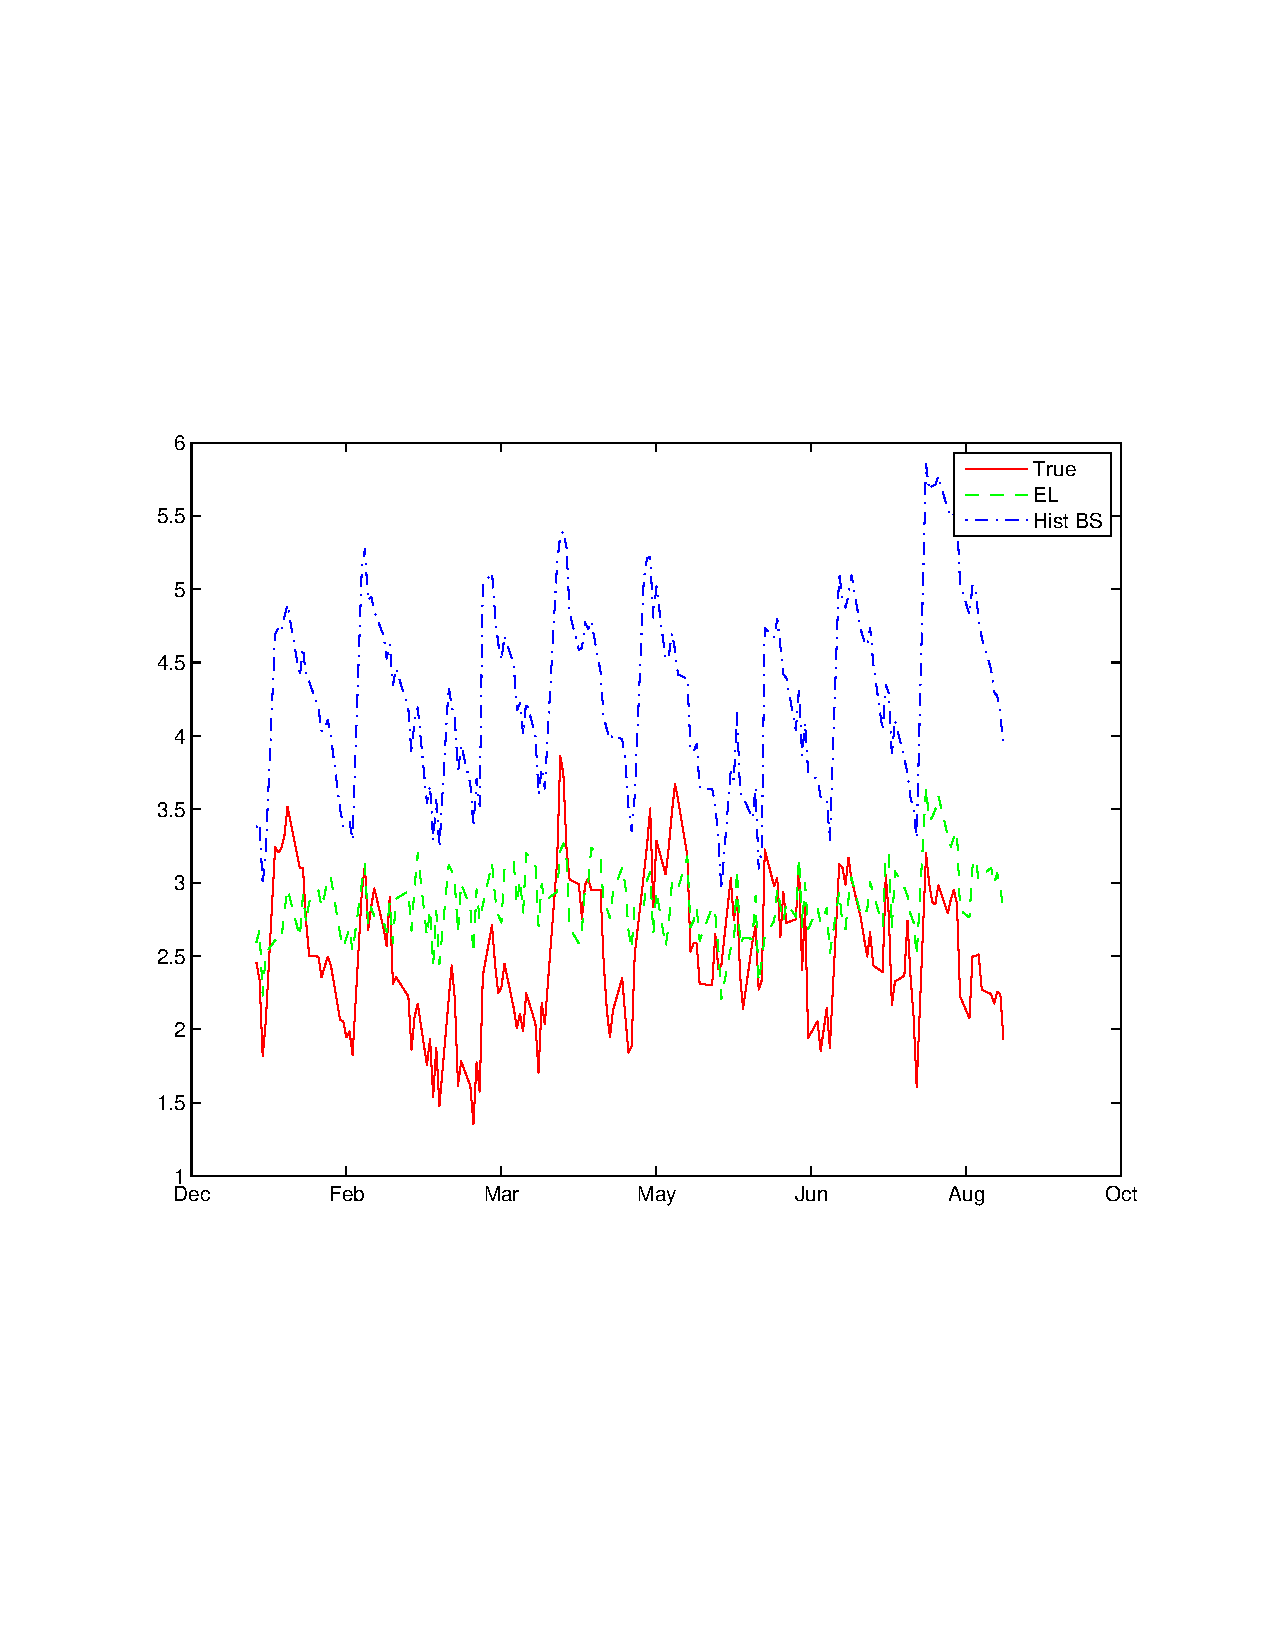
\includegraphics[width=0.8\textwidth]{SP500.pdf}
\end{figure}



\chapter{Approximate Bayesian Computation via Sufficient Dimension Reduction}

\setcounter{assumption}{0}
\section{Introduction}

There are two main objectives of this article. First, we want to provide
some theoretical results related to the currently emerging topic of
approximate Bayesian computation (ABC). The second is to show some
connectivity between ABC and another important emerging topic of research,
namely, sufficient dimension reduction (SDR). While the latter has
surfaced primarily in the{} frequentist's{}
domain of research, it is possible to tie it with ABC as well. In
particular, we want to show how ABC can be carried through nonlinear
SDR. 

Modern science invokes more and more Byzantine stochastic models,
such as stochastic kinetic network (\citet{wilkinson2011stochastic}),
differential equation system (\citet{picchini2014inference}) and
multi-hierarchical model (\citet{jasra2012filtering}), whose computational
complexity and intractability challenge the application of classical
statistical inference. Traditional maximum likelihood methods will
malfunction when the evaluation of likelihoods becomes slow and inaccurate.
Lack of analytical form of the likelihood also  {undermines
} the usage of Bayesian inferential tools, such as Markov chain Monte
Carlo (MCMC), Laplace approximation (\citet{tierney1986accurate}),
variational Bayes (\citet{jaakkola2000bayesian}) and posterior expansion
(\citet{johnson1970asymptotic}, Zhong and Ghosh%
\begin{comment}
need ask
\end{comment}
). 

The ABC methodology  {stems from} the observation
that the interpretability of the candidate model usually leads to
an applicable sampler of data given parameters, and ingeniously circumvents
the evaluation of likelihood functions. The idea behind ABC can be
summarized as follows: 
\begin{algorithm}[H]
\begin{enumerate}
\item Sample parameters $\theta_{i}$ from the prior distribution $\pi\left(\theta\right)$;
\item Sample data $Z_{i}$ based on the model $f\left(z\mid\theta_{i}\right)$;
\item Compare the simulated data $Z_{i}$ and the observed data $X_{i,\mathrm{obs}}$,
to accept or reject $\theta_{i}$.
\end{enumerate}
\protect\caption{Idea of ABC}
\end{algorithm}
 \citet{rubin1984bayesianly} first mentioned this idea and \citet{tavare1997inferring}
proposed the first version of ABC, which studying population genetics.
The prototype of ABC in recent research was given in \citet{pritchard1999population},
where the comparison of two data sets was simplified to a comparison
of summary statistics $S$ and the accept-reject decision was made
up to a certain error tolerance. 
\begin{algorithm}[h]
\begin{enumerate}
\item Sample parameters $\theta_{i}$ from the prior distribution $\pi\left(\theta\right)$;
\item Sample data $Z_{i}$ based on the model $f\left(z\mid\theta_{i}\right)$;
\item Accept $\theta_{i}$ if $\rho\left(S\left(Z_{i}\right),S\left(X_{\mathrm{obs}}\right)\right)\le\varepsilon$, {{}
} {for some metric $\rho$} {.}
\end{enumerate}
\protect\caption{\label{alg:Prichard-ABC-1}Prichard's Modified ABC}
\end{algorithm}
We can view this algorithm as a modified version of accept-reject
algorithm (\citet{robert2013monte}). The posterior is sampled by
altering the frequency of the proposal distribution, that is, the
prior. Now the full posterior distribution is approximated by the
following two steps (\citet{fearnhead2012constructing}): 
\begin{equation}
\pi\left(\theta\mid X_{\mathrm{obs}}\right)\approx\pi\left(\theta\mid S_{\mathrm{obs}}\right)\approx\pi\left(\theta\mid S_{\mathrm{sim}}\in O\left(S_{\mathrm{obs}},\varepsilon\right)\right),\label{eq:two-step-approx-abc}
\end{equation}
where $O\left(S_{\mathrm{obs}},\varepsilon\right)$ means a neighborhood
defined by the comparison measure $\rho$ and tolerance level $\varepsilon$.
We may note that the first approximation is exact when $S$ is sufficient.
Allowing the summary statistics to vary in an acceptable range sacrifices
a little accuracy in exchange for a significant improvement in computational
efficiency, which {makes } the algorithm more practical
and user-friendly. 

Pursuant to Algorithm \ref{alg:Prichard-ABC-1}, there are multiple
generalizations in the statistical literatures. \citet{marjoram2003markov}
{introduced } MCMC-ABC algorithm to concentrate the
samples in high posterior probability region, thereby increasing the
accept rate. Noisy ABC, proposed by \citet{wilkinson2013approximate},
makes use of all the prior samples by assigning kernel weights instead
of hard-threshold accept-reject mechanism and hence reduces the computational
burden. This perspective is corroborated in \citet{fearnhead2012constructing}
by convergence of Bayesian estimators. When the dependence structure
between hierarchies is intractable, ABC filtering technique innovated
by \citet{jasra2012filtering} comes to the rescue. Later in \citet{dean2014parameter},
a consistency argument is established for the specific case of hidden
Markov models. Moreover, many ABC algorithm above can be easily coded
in a parallel way, and hence take advantages of modern CPU, GPU structures.
This feature makes ABC algorithms extremely time-saving against long-established,
looping-based MCMC and MLE algorithms. 

Despite the fruitful results on ABC both from applied and theoretical
points of view. However, there exist only a handful of papers which
focus on the effect of the choice of summary statistics on the approximation
quality. The quintessential case is the summary statistics are sufficient,
and the resultant ABC sampler produces exact samples from the true
posterior distribution when $\varepsilon$ goes to zero. Nevertheless,
in a labyrinthine model, it is difficult to extract sufficient statistics,
except for some very special case, such as exponential random graph
models (e.g. \citet{grelaud2009abc}). \citet{joyce2008approximately}
proposed a concept called $\varepsilon-$sufficient to quantify the
effect of statistics. Nonetheless, this property is also difficult
to verify in complicated models. If we are interested only in model
selection, \citet{prangle2014semi} designs a semi-automatic algorithm
to construct summary statistics via logistic regression. And laterly,
\citet{marin2014relevant} gives sufficient conditions on summary
statistics in order to choose the right model based on the Bayes factor.
They advocate that the ideal summary statistics are ancillary in both
model candidates. One of our contribution comes from the mathematical
analysis of the consequence of conditioning the parameters of interest
on consistent statistics and intrinsically inconsistent statistics,
and appraises the efficiency of the posterior approximation based
on the former. Generally speaking, using consistent statistics results
in right concentration of the approximate posterior, while less efficiency
of statistics leads to less efficiency of approximation. One byproduct
is our theorem vindicates the usage of the posterior mean as summary
statistics as in \citet{fearnhead2012constructing}. 

In addition to the pure theoretical contribution, we also extend the{}
{two-step}{} algorithm in \citet{fearnhead2012constructing}
in a more flexible and nonparametric way for automatic constructing
summary statistics. We borrow the idea from another thriving topic,
namely sufficient dimension reduction (SDR). The motivation of SDR
which generalizes the concept of sufficient statistics is to estimate{}
{a} transformation $\varphi$, either{}
linear or nonlinear, such that 
\begin{equation}
Y\independent X\mid\varphi\left(X\right).\label{eq:sdr}
\end{equation}
 The first SDR method titled sliced inverse regression dates back
to \citet{li1991sliced}, followed by principle Hessian direction
in \citet{li1992principal} and also by \citet{1991}, and \citet{cook1998principal}.
As we step in the era of big data, this idea leads to a sea of papers
on both linear and nonlinear, predictor and response. Among the more
recent work, we refer to \citet{cook2002dimension}, \citet{xia2002adaptive},
\citet{li2005contour}, \citet{li2009dimension}, \citet{wu2008kernel},
\citet{yeh2009nonlinear}, \citet{su2011partial} and \citet{su2012inner}.
The association between SDR and ABC relies on the shared mathematical
formulation. If we think $\theta$ as the response and $X$ as the
predictor, then an ideal summary statistics $S\left(X\right)$ will
give 
\[
\theta\independent X\mid S\left(X\right).
\]
This simple observation offers raison d'etre to use existing SDR methods
in constructing summary statistics. The employment of dimension reduction
methods in our algorithm is different from that in \citet{blum2013comparative}.
In \citet{blum2013comparative}, dimension reduction methods, such
as best subset selection, projection techniques and regularization
approaches, are applied to reduce the dimension of existing summary
statistics, but here, we try to reduce the size of the original data.
Particularly in our paper, we incorporate the principal  support vector
machine for nonlinear dimension reduction given in \citet{li2011principal}
into ABC, which uses the{} {principal
} component of support vectors in reproducing kernel Hilbert space
(RKHS) as a nonparametric estimator of $\varphi$. 

The outline of remaining sections is as follows. Section \ref{sec:asymp-partial-post}
contains asymptotic results on the partial posterior. We gradually
relax the restriction on summary statistics and investigate the relationship
between the partial posterior and the full posterior. As a side result,
we give a lemma building a bridge between the recent prior free inferential
model (\citet{martin2013inferential} and \citet{martin2015conditional})
and traditional Bayesian inference. Section \ref{sec:abc-sdr} elicits
a new ABC algorithm which automatically produces summary statistics
through nonlinear SDR. A simulation result is provided in this section{}
{as well}. Section \ref{sec:Discussion} briefly
discusses the results and points out some possible future generalizations.


\section{\label{sec:asymp-partial-post}Asymptotic Properties of Partial Posterior}

Suppose $X_{1},\ldots,X_{n}\mid\theta$ are i.i.d. with common PDF
$f\left(x\mid\theta\right)$, and there exists a true but unknown
value $\theta_{0}$. Without loss of generality, we assume $\theta\in\mathbb{R}$,
and all probability density functions are with respect to the Lebesgue
measure. For illustration purpose, we define the following terminology.
\begin{defn}[Partial Posterior]
Let $S=S\left(X_{1},\ldots,X_{n}\right)$ be{} {statistics
} of the data. Given a prior $\pi\left(\theta\right)$,
we call the distribution 
\[
\pi\left(\theta\mid S\right)\propto\pi\left(\theta\right)g\left(S\mid\theta\right)
\]
the partial posterior, where $g\left(S\mid\theta\right)$ is the probability
density function of statistic $S\left(X_{1},\ldots,X_{n}\right)$
derived from the data density, and correspondingly, 
\[
\pi\left(\theta\mid X_{1},\ldots,X_{n}\right)\propto\pi\left(\theta\right)f\left(X_{1},\ldots,X_{n}\mid\theta\right)
\]
 is called the full posterior.
\end{defn}
From equation (\ref{eq:two-step-approx-abc}), partial posterior significantly
reduces the complexity of full posterior by replacing the dependence
on full data by lower dimensional statistics $S$. If the partial
posterior deviates from {the } full
posterior too much, then no matter how delicately we sample from $\pi\left(\theta\mid S_{\mathrm{sim}}\in O\left(S_{\mathrm{obs}},\varepsilon\right)\right)$
, how small $\varepsilon$ we choose, the resultant samples would
not behave like ones drawn from the original full posterior, which {makes } the subsequent Bayesian analysis fragile
and unreliable. Therefore, theoretical connection between some easily
verifiable properties and asymptotic behaviour of partial posterior
is of relevance. In particular, we want to study consistency and asymptotic
normality of our Bayesian procedures. The following theorems try to
demonstrate the connection between the asymptotic behaviour of summary
statistics and that of partial posterior. We start from the most popular
statistics, the maximum likelihood estimator (MLE) of $\theta$. 
\begin{thm}
\label{thm:bernstein-von-mises-mle}Let $\hat{\theta}$, the MLE of
$\theta$, be a strongly consistent estimator, and let $\hat{I}$
be the observed Fisher information evaluated at $\hat{\theta}$, and
the full posterior holds Bernstein--von Mises theorem. Then for any
$\varepsilon>0$, and any $t$, the partial posterior after conditioned
on $\hat{\theta}$ satisfies 
\[
\lim_{n\rightarrow\infty}P\left(\sqrt{n\hat{I}}\left(\theta-\hat{\theta}\right)\le t\mid\hat{\theta}\in O\left(\theta_{0},\varepsilon\right)\right)=\Phi\left(t\right),\ascv.
\]
\end{thm}
\begin{proof}
See  \ref{sec:proof-thm-1}.\end{proof}
\begin{rem}
There is a slight difference between 
\[
\lim_{n\rightarrow\infty}P\left(\sqrt{n\hat{I}}\left(\theta-\hat{\theta}\right)\le t\mid\hat{\theta}\in O\left(\theta_{0},\varepsilon\right)\right)=\Phi\left(t\right),\ascv.\left(P_{\theta_{0}}\right)
\]
and 
\[
\lim_{n\rightarrow\infty}P\left(\sqrt{n\hat{I}}\left(\theta-\hat{\theta}\right)\le t\mid\hat{\theta}\right)=\Phi\left(t\right),\ascv.
\]
By definition, 
\begin{equation}
P\left(\sqrt{n\hat{I}}\left(\theta-\hat{\theta}\right)\le t\mid\hat{\theta}\right)=\lim_{\varepsilon\rightarrow0}\frac{P\left(\sqrt{n\hat{I}}\left(\theta-\hat{\theta}\right)\le t,\hat{\theta}\in O\left(s,\varepsilon\right)\right)}{P\left(\hat{\theta}\in O\left(s,\varepsilon\right)\right)}.\label{eq:def-loose-partial-post}
\end{equation}
The result of Theorem \ref{thm:bernstein-von-mises-mle} can only
be used to prove 
\[
\lim_{\varepsilon\rightarrow0}\lim_{n\rightarrow\infty}P\left(\sqrt{n\hat{I}}\left(\theta-\hat{\theta}\right)\le t\mid\hat{\theta}\in O\left(\theta_{0},\varepsilon\right)\right)=\Phi\left(t\right),\ascv,
\]
switching order of limits in equation (\ref{eq:def-loose-partial-post}). 
\begin{rem}
The definition of $P\left(\theta\mid\hat{\theta}\in O\left(\theta_{0},\varepsilon\right)\right)$
is different from the approximation $P\left(\theta\mid\hat{\theta}\in O\left(\hat{\theta}_{\mathrm{obs}},\varepsilon\right)\right)$.
In former case, $\hat{\theta}$ is evaluated at $X_{1},\ldots,X_{n}\sim\pi\left(x\mid\theta_{0}\right)$,
the observed data, while the latter evaluates $\hat{\theta}$ at $Z_{1},\ldots,Z_{m}\sim\pi\left(z\mid\theta\right)$,
the simulated data. 
\end{rem}
\end{rem}
By {assumptions }, the asymptotic
distribution of the full posterior is still normal, and we have 
\begin{eqnarray*}
 &  & \sup_{t\in\mathbb{R}}\left|P\left(\sqrt{n\hat{I}}\left(\theta-\hat{\theta}\right)\le t\mid\hat{\theta}\in O\left(\theta_{0},\varepsilon\right)\right)-P\left(\sqrt{n\hat{I}}\left(\theta-\hat{\theta}\right)\le t\mid X_{1},\ldots,X_{n}\right)\right|\\
 & \le & \sup_{t\in\mathbb{R}}\left|P\left(\sqrt{n\hat{I}}\left(\theta-\hat{\theta}\right)\le t\mid\hat{\theta}\in O\left(\theta_{0},\varepsilon\right)\right)-\Phi\left(t\right)\right|+\sup_{s\in\mathbb{R}}\left|P\left(\sqrt{n\hat{I}}\left(\theta-\hat{\theta}\right)\le s\mid X_{1},\ldots,X_{n}\right)-\Phi\left(s\right)\right|\\
 & \le & 2\varepsilon\rightarrow0,\left(n\rightarrow\infty\right).
\end{eqnarray*}
Hence, we can informally say that two random variables $\sqrt{n\hat{I}}\left(\theta-\hat{\theta}\right)\mid\hat{\theta}$
and $\sqrt{n\hat{I}}\left(\theta-\hat{\theta}\right)\mid X_{1},\ldots,X_{n}$
are close in distribution. Note that both random variables asymptotically
center at consistent MLE, and hence will eventually concentrate at
$\theta_{0}$. Meanwhile, the scale factors in both random variables
are $\sqrt{n\hat{I}}$, which {ensures
} the same square root credible  {intervals}.
In this sense, we feel that the partial posterior conditioned on MLE
has the same efficiency as the full posterior. Later theorems will
tell us that if the summary statistics are not efficient, the corresponding
partial likelihood will have a different scale factor, and thus lose
efficiency and result in a larger credible interval. 

A slightly modified proof of Theorem \ref{thm:bernstein-von-mises-mle}
can be used to support the posterior mean as a summary statistic in
\citet{fearnhead2012constructing} and we still have a similar result,
namely 
\[
\lim_{n\rightarrow\infty}P\left(\sqrt{n\hat{I}}\left(\theta-E\left(\theta\mid X_{1},\ldots,X_{n}\right)\right)\le t\mid E\left(\theta\mid X_{1},\ldots,X_{n}\right)\in O\left(\theta_{0},\varepsilon\right)\right)=\Phi\left(t\right),\ascv.
\]
The key fact to support the assert above comes from \citet{ghosh2011moment},
that is, the higher order closeness of the posterior mean and the
MLE, 
\begin{equation}
\lim_{n\rightarrow\infty}\sqrt{n}\left(E\left(\theta\mid X_{1},\ldots,X_{n}\right)-\hat{\theta}\right)=0,\ascv.\label{eq:high-order-close-post-mean-mle}
\end{equation}
Indeed, any estimator who has the same or higher order of closeness
to MLE will work as an efficient summary statistic.

Theorem \ref{thm:bernstein-von-mises-mle} can be generalized to more
intricate models. The following example shows the same phenomenon
in data generated from a Markov process.
\begin{example}
\label{exa:Immigrate-emigrate-process}Immigration-emigration process
is {a } crucial
model in survival analysis and can be viewed as a special case of
mass-action stochastic kinetic  {network
} (\citet{wilkinson2011stochastic}). The model is defined by a birth
procedure and {a } death
procedure during an infinitesimal time interval, namely, 
\[
P\left(X\left(t+\diff t\right)=x_{1}\mid X\left(t\right)=x_{0}\right)=\begin{cases}
\lambda\diff t+o\left(\diff t\right), & x_{1}=x_{0}+1,\\
\mu x_{0}\diff t+o\left(\diff t\right), & x_{1}=x_{0}-1,\\
1-\lambda\diff t-\mu x_{0}\diff t+o\left(\diff t\right), & x_{1}=x_{0}.
\end{cases}
\]
Assume that we observe full data in the time interval $\left[0,T\right]$.
Let $T_{i},i=1,\ldots,n$ be the event times and $X_{i}=X\left(T_{i}\right),i=1,\ldots,n$.
Let $X_{0}$ be initial population, $T_{0}=0$, $T_{n+1}=T$. Then
by Gillespie's algorithm, the likelihood is proportional to 
\[
\lambda^{r_{1}}\exp\left(-\lambda T\right)\mu^{r_{2}}\exp\left(-\mu A_{T}\right),
\]
where $r_{1}$ and $r_{2}$ are number of events corresponding to
immigration and emigration, and 
\[
A_{T}=\int_{0}^{T}X\left(t\right)\diff t.
\]
The MLEs are 
\[
\hat{\lambda}=\frac{r_{1}}{T},\hat{\mu}=\frac{r_{2}}{A_{T}},
\]
and they are strongly consistent estimators of $\lambda$ {and $\mu$} when $T$ goes to
infinity. By the computation in  \ref{sub:Derivation-of-Example-1},
we have the partial posterior density function of $\sqrt{T}\left(\mu-\hat{\mu}\right)$
conditioned on $\hat{\mu}$, $r_{1}$ and $T$ given by 
\[
\lim_{T\rightarrow\infty}\pi\left(\sqrt{T}\left(\mu-\hat{\mu}\right)=t\mid\hat{\mu},r_{1},T\right)=\frac{\hat{\mu}}{\sqrt{2\pi\hat{\lambda}}}\exp\left(-\frac{\hat{\lambda}}{\hat{\mu}^{2}}t^{2}\right),\ascv.
\]

\end{example}
The MLE seems to be a perfect surrogate for  {the
} full data. However, in many cases, use of MLE is
prohibitive due to heavy computational burden, particularly when the
likelihood function is intractable. This is when the ABC comes on
stage. $M$-estimator is a generalization of the MLE, which is also
consistent and asymptotically normal under mild conditions. Many $M$-estimators
can be easily calculated, especially some moment estimators. To give
an idea of the nature of approximation, we consider the following
examples.
\begin{example}
\label{exa:Gamma-distribution}Gamma distribution can be used to model
hazard functions in survival analysis. The shape parameter of gamma
distribution determines the trend of hazard and hence is a vital parameter
to estimate. Assume $X_{1},\ldots,X_{n}\sim\mathrm{Gamma}\left(\alpha,\beta\right)$,
where we know the scale parameter $\beta$, but not the shape parameter
$\alpha$. The MLE of $\alpha$ is the solution of 
\[
-\log\Gamma\left(\alpha\right)-\alpha\log\beta+\left(\alpha-1\right)\sum_{i=1}^{n}\log X_{i}-\frac{\sum_{i=1}^{n}X_{i}}{\beta}=0,
\]
which involves repeated evaluation of the gamma function in search
of the root. A simple $M$-estimator $\tilde{\alpha}=\overline{X}/\beta$
is derived from its mean equation, 
\[
\sum_{i=1}^{n}\left(X_{i}-\alpha\beta\right)=0.
\]
 Now we consider the partial posterior $\pi\left(\alpha\mid\tilde{\alpha}\right)$,
when the prior is $\pi\left(\alpha\right)\propto\exp\left(-\lambda\alpha\right)$.
By the calculation in  \ref{sub:Derivation-of-Example-2}, we show
that the limit of cumulative probability function of $\sqrt{n}\tilde{\alpha}^{-1}\left(\alpha-\tilde{\alpha}\right)$
given $\tilde{\alpha}$ is 
\[
\lim_{n\rightarrow\infty}P\left(\sqrt{n}\tilde{\alpha}^{-1}\left(\alpha-\tilde{\alpha}\right)\le t\mid\tilde{\alpha}\right)=\Phi\left(t\right),\ascv,
\]
which means that the Bernstein-von Mises theorem holds for the partial
posterior conditioned on the $M$-estimator $\tilde{\alpha}$. The
scale factor of   the partial posterior is $\sqrt{n}\tilde{\alpha}^{-1}$,
which is smaller than that of {the
} full posterior, $\sqrt{n\psi'\left(\alpha\right)}$,
where $\psi\left(\alpha\right)$ is digamma function. That results
in a larger credible interval based on the partial posterior. 
\begin{example}
\label{exa:laplace-example}Another example is Laplace distribution
with PDF 
\[
f_{\mu,\lambda}\left(t\right)=\frac{1}{2\lambda}\exp\left(-\frac{\left|t-\mu\right|}{\lambda}\right).
\]
 Here we want inference the location parameter $\mu$ holding $\lambda$
fixed. The MLE is the {the } sample
median and the moment estimator is {the
}sample mean. Here we calculate the partial posterior based on sample
mean. By the calculation in  \ref{sub:Derivation-of-Example-3}, we
find that the characteristic function of $\sqrt{n}\left(\mu-\overline{X}\right)$
converges to $\exp\left(-\lambda^{2}t^{2}\right)$, which is the characteristic
function of normal distribution. 
\end{example}
\end{example}
Example \ref{exa:laplace-example} uses the following lemma which
is of independent interest. 
\begin{lem}
\label{lem:bayes-inferential-model}Assume $X$ has the same distribution
as $h\left(Y,\theta\right)$, where $h$ is a function one-to-one
in $\theta$ and $Y$ is a random variable independent of $\theta$.
Let $\theta=g\left(y,x\right)$ and $y=u\left(x,\theta\right)$ be
the solutions of equation $x=h\left(y,\theta\right)$. Further assume
$\partial u\left(x,\theta\right)/\partial x$ exists and is not equal
to zero. Then the posterior distribution of $\theta$ conditioned
on $X$ under the uniform prior has the same distribution as $g\left(Y,x\right)$,
where $x$ is fixed. \end{lem}
\begin{rem}
Although not quite related to ABC, this lemma gives another interpretation
of inferential model of \citet{martin2013inferential} and \citet{martin2015conditional}.
In their settings, $Y$ is called unobserved ancillary variable, and
$g\left(y,x\right)$ is $\Theta_{x}\left(u\right)$ in their notation.
They claim that their procedure results in a distribution of $\theta$
without referring to a prior. However, by our lemma, this model is
mathematically the same as a posterior given a uniform prior.
\end{rem}
The following theorems are built upon the Theorem 2.1 in \citet{rivoirard2012bernstein},
which guarantees the asymptotic normality of linear functionals of
nonparametric posterior. So we need all the assumptions in that theorem.
Additionally, we need the following assumptions. 
\begin{assumption}
\label{assu:second-order-bounded-differential}There is a neighbourhood
$\theta\in O\left(\theta_{0},\varepsilon\right)$ such that $\int_{\mathbb{R}}g\left(x,\theta_{0}\right)\pi\left(x\mid\theta\right)\diff x$
is a continuous twice differentiable in $\theta$ and the second order
derivative is bounded by some constant $L$. 
\begin{assumption}
\label{assu:m-est-consistent-asymp-norml}$M$-estimator $\tilde{\theta}$
and MLE $\hat{\theta}$ are both strongly consistent and asymptotically
normal.
\begin{assumption}
\label{assu:bernstein-von-mises-full-posterior} Bernstein--von Mises
theorem and posterior consistency hold for the full posterior of $\theta$.
\begin{assumption}
\label{assu:theo-mle}For any $\theta\in\Theta$, $E_{\theta_{0}}\log f\left(X\mid\theta\right)\le E_{\theta_{0}}\log f\left(X\mid\theta_{0}\right)$. 
\end{assumption}
\end{assumption}
\end{assumption}
\end{assumption}
Now we can articulate the theorem. 
\begin{thm}
\label{thm:partial-post-m-est}Under the Assumptions \ref{assu:second-order-bounded-differential},
\ref{assu:m-est-consistent-asymp-norml}, \ref{assu:bernstein-von-mises-full-posterior},
\ref{assu:theo-mle}, and conditions of Theorem 2.1 in \citet{rivoirard2012bernstein},
for any $\varepsilon$ and $t$, 
\[
\lim_{n\rightarrow\infty}P\left(\left.\frac{\sqrt{n}\left(\theta-\tilde{\theta}\right)}{\sqrt{\tilde{V}}}\le t\right|\tilde{\theta}\in O\left(\theta_{0},\varepsilon\right)\right)=\Phi\left(t\right),\ascv,
\]
where $\tilde{V}=V_{0}/G_{1}\left(\tilde{\theta},\tilde{\theta}\right)^{2}$
is Godambe information. \end{thm}
\begin{proof}
See  \ref{sec:Proof-of-Theorem-2}.
\end{proof}
Using similar arguments as Theorem \ref{thm:bernstein-von-mises-mle},
the partial posterior $\sqrt{n\tilde{V}^{-1}}\left(\theta-\tilde{\theta}\right)\mid\tilde{\theta}$ {{}
} {is asymptotically } close in distribution to  {the
}full posterior $\sqrt{n\hat{I}}\left(\theta-\hat{\theta}\right)\mid X_{1},\ldots,X_{n}$.
Since both the $M$-estimator and the MLE are strongly consistent,
the partial posterior still concentrates around the right $\theta_{0}$,
but now the asymptotic $\alpha-$level credible interval based on
the partial posterior, namely 
\[
\left(\tilde{\theta}-Z_{\alpha/2}\sqrt{\frac{\tilde{V}}{n}},\tilde{\theta}+Z_{\alpha/2}\sqrt{\frac{\tilde{V}}{n}}\right),
\]
will be larger than that based on the full posterior, 
\[
\left(\hat{\theta}-Z_{\alpha/2}\sqrt{\frac{\hat{I}^{-1}}{n}},\hat{\theta}+Z_{\alpha/2}\sqrt{\frac{\hat{I}^{-1}}{n}}\right),
\]
where $Z_{\alpha/2}$ is $\left(1-\alpha/2\right)$ quantile of standard
normal distribution, because the Godambe information $\tilde{V}^{-1}$
is typically no larger than Fisher information $\hat{I}$. Hence,
we lose efficiency if we condition the posterior on an inefficient
estimator, which coincides our intuition.

For extreme tortuous models, even finding a consistent estimator can
be quite hard. There are still some simple statistics which may be
consistent to some {{} } {functions } of
$\theta$. Unless they are ancillary statistics, they always contain
some information about the {{} } {parameters
} of interest. Moreover, in real case, we use several statistics,
each of which gives independent information of the full posterior.
In the remainder of this section, we will mathematically qualify what
independent information means and show that using more than one statistic
will improve the efficiency. 

Let $S_{i}$, $i=1,\ldots,q$ be statistics of the sample. We make
the following trivial assumptions. 
\begin{assumption}
\label{assu:joint-normal-inconsist-stat}The joint distribution of
$S_{1},\ldots,S_{q}$ converges in distribution to a multivariate
normal distribution $N\left(h\left(\theta_{0}\right),n^{-1/2}\Sigma\left(\theta_{0}\right)\right)$,
and each $S_{i}$ converges to $h_{i}\left(\theta_{0}\right)$ almost
surely. Further, assume $\Sigma\left(\theta_{0}\right)$ {{}
}\textcolor{black}{is } positive definite, and $h\left(\theta_{0}\right)$
is a linear functional of the distribution function, that is 
\[
h\left(\theta_{0}\right)=\int_{\mathbb{R}}g\left(x\right)f\left(x\mid\theta_{0}\right)\diff x,
\]
where $g\left(x\right)\in\mathbb{R}^{q}$. 
\end{assumption}
Assumption \ref{assu:joint-normal-inconsist-stat} characterizes the
 independent information statement. Because if $\Sigma\left(\theta_{0}\right)$
has a lower rank, then some of $S_{i}$ can be expressed as \textcolor{black}{
}linear combinations of {{} }\textcolor{black}{other } $S_{j}$
asymptotically. Then the partial posterior can be reduced to a partial
posterior based solely on the $S_{j}$. The functional form of $h$ is
a natural consequence when we apply some version of strong law of
large numbers to prove convergence of statistics. 

In order to prove the theorem, we need some more technical assumptions.
\begin{assumption}
\label{assu:super-strong-consistent}Let $S=\left(S_{1},\ldots,S_{q}\right)$,
assume 
\[
\lim_{n\rightarrow\infty}n^{1/2}\left\{ \frac{1}{n}\sum_{i=1}^{n}g\left(X_{i}\right)-S\right\} =0,\ascv.
\]
and there exists a strongly consistent estimator $\tilde{\Sigma}$
of $\Sigma\left(\theta_{0}\right)$
\end{assumption}
Only Assumption \ref{assu:super-strong-consistent} seems quite restrictive.
Based on all these assumptions, the theorem describing the partial
posterior conditioned on less informative statistics can be found
as follows:
\begin{thm}
\label{thm:bernsten-von-mise-inconsist-multv}Under the Assumptions
\ref{assu:joint-normal-inconsist-stat},
\ref{assu:super-strong-consistent} and conditions of Theorem 2.1
in \citet{rivoirard2012bernstein}, for any vector $a\in\mathbb{R}^{q}$,
\[
\lim_{n\rightarrow\infty}\sup_{t\in\mathbb{R}}\left|P\left(\left.\frac{\sqrt{n}a^{T}\left(h\left(\theta\right)-S\right)}{\sqrt{a^{T}\tilde{\Sigma}a}}\le t\right|S\right)-\Phi\left(t\right)\right|=0,\ascv.
\]
\end{thm}
\begin{proof}
See \ref{sec:Proof-of-Theorem-3}.
\end{proof}
Theorem \ref{thm:bernsten-von-mise-inconsist-multv} extends the asymptotic
results about $M$-estimators to more general statistics, particularly
the intrinsically inconsistent statistics defined as follows.
\begin{defn}[Intrinsic Consistency]
Let $S$ be an non-ancillary statistic and converges to $h\left(\theta_{0}\right)$
almost surely. If $h\left(\cdot\right)$ is an one-to-one function
and has an inverse function, then we say $S$ is intrinsically consistent.
Otherwise, we say $S$ is intrinsically inconsistent. 
\end{defn}
If $S$ is a one dimensional intrinsic inconsistent statistic, then
Theorem \ref{thm:bernsten-von-mise-inconsist-multv} asserts the $\left(1-\alpha\right)$
asymptotic credible set based on {{} } {the
} partial posterior is 
\[
\left\{ \theta:S-Z_{\alpha/2}\sqrt{\frac{\tilde{\Sigma}}{n}}\le h\left(\theta\right)\le S+Z_{\alpha/2}\sqrt{\frac{\tilde{\Sigma}}{n}}\right\} .
\]
In an extreme case, when sample size $n$ is large enough, such that
$Z_{\alpha/2}/\sqrt{n}\approx0$, the asymptotic credible interval
by {{} } {the } full posterior would be
close to the singleton $\left\{ \hat{\theta}\right\} $. However,
the credible set based on {{} } {the } partial
posterior would be $\left\{ \theta:h\left(\theta\right)=S\right\} $.
By the definition of intrinsic inconsistency, $h$ is not a one-to-one
function. Then the set $\left\{ \theta:h\left(\theta\right)=S\right\} $
would possibly hold multiple elements, hence larger than that from {{}
} {the } full posterior. Again, in this sense, we
perceive loss of efficiency due to conditioning the posterior on arbitrary
statistics. 

Another interesting use of Theorem \ref{thm:bernsten-von-mise-inconsist-multv}
is a more pragmatic asymptotic assessment of effectiveness of including {{}
} {many} statistics than that in \citet{joyce2008approximately}.
In their settings, the effectiveness of summary statistics is measured
by the difference between log-likelihoods, thus not operable when
likelihood  {{} functions are} intractable. On the other
hand, our approach only {{} } {requires
}the asymptotic behaviour of statistics, and the corresponding credible
set with $q$ statistics can be developed by Cremer%
\begin{comment}
ask Ghosh
\end{comment}
{} device as 
\[
\left\{ \theta:n\left(h\left(\theta\right)-S\right)^{T}\tilde{\Sigma}\left(h\left(\theta\right)-S\right)\le\chi_{1-\alpha,q}^{2}\right\} ,
\]
where $\chi_{1-\alpha,q}^{2}$ is $\left(1-\alpha\right)$ quantile
of chi-square distribution with degree of freedom $q$. To select
summary statistics, we can compare the asymptotic credible sets with
and without the current statistic. If the difference is small, then
we can safely throw the current statistic away. 

The following is a simple example to illustrate this phenomenon.
\begin{example}
\textcolor{black}{Let $X_{i}$ are i.i.d. sample from $N\left(\mu,\mu^{2}\right)$
and we calculate the partial posterior $\pi\left(\mu\mid s^{2}\right)$,
where $s^{2}$ is the sample standard deviation.  The prior of $\mu^{2}$
is assumed to be inverse gamma distribution with shape parameter $\alpha$
and scale parameter $\beta$. We know the $s^{2}\sim\mu^{2}\chi_{n-1}^{2}/\left(n-1\right)$,
hence the partial posterior of $\mu^{2}$ conditioning on $s^{2}$
is an inverse gamma distribution with shape parameter $\left\{ \alpha-1+\left(n-1\right)/2\right\} $
and scale parameter $\left\{ \beta+\left(n-1\right)s^{2}/2\right\} $.
This leads to a bimodal partial posterior for $\mu$. Hence, we can
only get the absolute value of $\mu$ without sign information from
this partial posterior.}
\end{example}

\section{\label{sec:abc-sdr}Approximate Bayesian Computation {{}
} {via } Nonlinear Sufficient Dimension Reduction}

In principle, almost all the existing dimension reduction methods
are valid in estimating the summary statistics. However, there is
a slight difference between the setting of SDR and ABC. In the theory
of SDR, the independent assumption \ref{eq:sdr} must hold rigorously,
which implies $Y\mid X$ has exactly the same distribution as $Y\mid S\left(X\right)$.
However, by our Theorem \ref{thm:bernstein-von-mises-mle}, \ref{thm:partial-post-m-est}
and \ref{thm:bernsten-von-mise-inconsist-multv}, the two distributions
are only close in large but finite sample. 

In our paper, we choose principal support vector machine in \citet{li2011principal}.
Suppose we have a regression problem $\left(Y_{i},X_{i}\right)$,
and search a nonlinear transformation $\varphi:\mathbb{R}^{p}\rightarrow\mathbb{R}^{d}$,
such that $Y\independent X\mid\varphi\left(X\right)$. Then the main
steps in principal support vector machine are given in Algorithm \ref{alg:Principal-Support-Vector}
. 

\begin{algorithm}
\begin{enumerate}
\item (Optional) Marginally standardize data $X_{1},\ldots,X_{n}$. The
purpose of this step is so that the kernel $\kappa$ treats different
components of $X_{i}$ more or less equally. 
\item Choose kernel $\kappa$ and the number of basis {{} } {functions
}$k$ (usually around $n/3\sim2n/3$). Compute $K=\left(\kappa\left(X_{i},X_{j}\right)\right)_{n\times n}$.
Let $Q=I_{n}-J_{n}/n$, where $J_{n}$ is the $n\times n$ matrix
whose entries are 1. Compute largest $k$ eigenvalues $\lambda_{1},\ldots,\lambda_{k}$
and corresponding eigenvectors $w_{1},\ldots,w_{k}$ of matrix $QKQ$.
Let $\Psi=\left(w_{1},\ldots,w_{k}\right)$ and $P_{\Psi}=\Psi\left(\Psi^{T}\Psi\right)^{-1}\Psi^{T}$
be the projection matrix onto $\Psi$.
\item \label{enu:svm}Partition the response variable space $Y$ into $h$
slices defined by $y_{1},\ldots,y_{h-1}$. For each $y_{s},\: s=1,\ldots,h-1$,
define a new response variable $\tilde{Y}_{si}=I_{\left[Y_{i}\le y_{s}\right]}-I_{\left[Y_{i}>y_{s}\right]}$.
Then solve the modified support vector machine problem as a standard
quadratic programming 
\[
\min_{\alpha}-1^{T}\alpha+\frac{1}{4}\alpha^{T}\mathrm{diag}\left(\tilde{Y}_{s}\right)P_{\Psi}\mathrm{diag}\left(\tilde{Y}_{s}\right)\alpha,
\]
subject to constraints
\[
\begin{cases}
0\le\alpha\le\lambda,\\
\tilde{Y}_{s}^{T}\alpha=0,
\end{cases}
\]
where $\mathrm{diag}\left(\tilde{Y}_{s}\right)$ is a diagonal matrix
using $\tilde{Y}_{s}$ as diagonal, $\lambda$ is a hyper-parameter
in ordinary support vector machine. The coefficients of support vectors
in RKHS {{} } {are} 
\[
c_{s}^{*}=\frac{1}{2}\left(\Psi^{T}\Psi\right)^{-1}\Psi^{T}\mathrm{diag}\left(\tilde{Y}_{s}\right)\alpha_{s}.
\]

\item \label{enu:pca}Let $d$ be the target dimension. Compute the eigenvectors
$v_{1},\ldots,v_{d}$ of first largest $d$ eigenvalues of the matrix
$\sum_{s=1}^{h-1}c_{s}^{*}c_{s}^{*T}$. Let $V=\left(v_{1},\ldots,v_{d}\right).$
\item Let $K\left(x,X\right)=\left(\kappa\left(x,X_{i}\right)-n^{-1}\sum_{j=1}^{n}\kappa\left(x,X_{j}\right)\right)$
be a $n$ dimensional vector. Then the estimated transformation $\hat{\varphi}\left(x\right)=V^{T}\left(\mathrm{diag}\left(\lambda_{1},\ldots\lambda_{k}\right)\right)^{-1}\Psi^{T}K\left(x,X\right).$
\end{enumerate}
\protect\caption{Principal Support Vector Machine\label{alg:Principal-Support-Vector}}
\end{algorithm}
By slicing the response variable space, we discretize variation of
$Y$. The support vector machine in Step \ref{enu:svm} recognizes
the robust separate hyperplanes. We will expect the variation of $Y$
along the directions within hyperplanes to be negligible and that
along the directions perpendicular to the hyperplanes the most part
of covariation between $Y$ and $X$ is explained. The principal component
analysis on the support vectors in Step \ref{enu:pca} estimates the {{}
} {principal } {{} }perpendicular directions
and hence creates the sufficient directions in RHKS. 

Based on Algorithm \ref{alg:Principal-Support-Vector}, we formulate
our  {two-step }approximate Bayesian computation algorithm
in Algorithm \ref{alg:ABC-via-PSVM}.

\begin{algorithm}
\begin{enumerate}
\item \label{enu:direct-sampling}Sample $\theta_{i}$ from the prior $\pi\left(\theta\right)$
and sample $X_{i1},\ldots,X_{in}$ from the model $f\left(x\mid\theta_{i}\right)$. 
\item View $\left(\theta_{i},X_{i1},\ldots X_{in}\right)$ as a multivariate
regression problem and reduce the dimension from $n$ to $d$ via
principal support vector machine. Denote the estimated transformation
as $\hat{S}\left(X_{1},\ldots,X_{n}\right)$. 
\item Either use existent samples in Step \ref{enu:direct-sampling} or
repeat it and get new sample. Calculate the estimated summary statistics
$\hat{S}_{i}=\hat{S}\left(X_{i1},\ldots,X_{in}\right)$ on each set
$X_{i1},\ldots,X_{in}$ corresponding to prior samples $\theta_{i}$.
Also calculate $\hat{S}_{\mathrm{obs}}=\hat{S}\left(X_{1},\ldots,X_{n}\right)$
on the observed data set.
\item Based on the metric $\rho\left(\hat{S}_{i},\hat{S}_{\mathrm{obs}}\right)$,
make the decision of accept or reject of $\theta_{i}$. 
\end{enumerate}
\protect\caption{\label{alg:ABC-via-PSVM}ABC via PSVM}
\end{algorithm}
Algorithm \ref{alg:ABC-via-PSVM} directly generalizes the semi-automatic
ABC in \citet{fearnhead2012constructing}. In their algorithm, the
summary statistics are fixed as posterior means and recommended the
estimation method is polynomial regression. Our algorithm relaxes
the restriction on summary statistics and{} lets
the data and nonparametric algorithm together find them adaptively.
One significant difference between our algorithm and the conventional
ABC is in Step \ref{enu:direct-sampling}, where each prior sample
$\theta_{i}$ produces exact $n$ simulated data, because the nonparametric
estimator of statistics should take $n$ arguments so that it can
be evaluated at both observed data and simulated data.
\subsection{Robustness of PSVM}

\textcolor{black}{The discrepancy between the asymptotic behavior
of ABC and settings in SDR requires new properties of PSVM, namely
robustness, which suggests that $\hat{\Gamma}$ from PSVM would be
in the vicinity of the true summary statistics function $\Gamma$
in some sense even if the partial posterior is only close to the full
posterior. Here is the theorem which validates this property.}
\begin{theorem}[Robustness of PSVM]
\textcolor{black}{\label{thm:robust-psvm} Assume 
\[
\lim_{n\rightarrow\infty}\sup_{s}\left|P\left\{ \theta\le s\mid\Gamma_{n}^{T}\left(X_{1},\ldots,X_{n}\right)\right\} -P\left(\theta\le s\mid X_{1},\ldots,X_{n}\right)\right|=0,
\]
where $\Gamma\in\mathbb{R}^{n\times d}$, with $d$ fixed. Further
assume all the conditions in Theorem 4 and 5 in \cite{li2011principal}. Let $\hat{\Gamma}_{n}$
be the result from PSVM. Then 
\[
\hat{\Gamma}_{n}-\Gamma_{n}\overset{p}{\rightarrow}0.
\]
}\end{theorem}
\begin{proof}
\textcolor{black}{See Appendix E. }
\end{proof}

\subsection{\textcolor{black}{Simulation Example }}

\textcolor{black}{First, we will show a simple simulation example
to illustrate the robustness of SVM, which serves as the foundation
of the robustness of PSVM.}
\begin{example}
\textcolor{black}{Let $\theta\mid X_{1},X_{2}\sim N\left(2X_{1}+X_{2}+0.001\left(X_{1}^{2}+X_{2}^{2}\right),1\right)$.
Hence the conditional distribution of $\theta$ on $X_{1},X_{2}$
is close to $N\left(2X_{1}+X_{2},1\right)$. Then the normal vectors
of sliced SVM should be in vicinity of $\left(2,1\right)$. We choose
the slicing point $s=1.5$. The results are summarized in Fig \ref{fig:Normal-Vectors-sliced-svm}.
The dots are normal vectors, the solid line is the principal component
direction of normal vectors, and the reference dashed line is $\psi_{1}=2\psi_{2}$.
We can see the principal component direction is quite close to the
reference line.}

\begin{figure}
{\includegraphics[scale=0.5]{normalVec}\protect\caption{\textcolor{black}{Normal Vectors of Separate Hyperplanes in Sliced
SVM}\label{fig:Normal-Vectors-sliced-svm}}
}

\end{figure}

\end{example}

Next, we will show a simple simulation example to illustrate our algorithm.

\begin{example}
Autoregressive model with lag one, AR(1). 
\[
Y_{i}=\beta Y_{i-1}+\varepsilon.
\]
Set $Y_{1}=1$ and number of observation is 100. Assume $\varepsilon\sim N\left(0,0.5^{2}\right)$,
true regression coefficient 0.6. We put uniform prior in $\left(-1,1\right)$
on $\beta$, then the true posterior distribution is $N\left(\sum_{i=1}^{99}Y_{i}Y_{i+1}/\left(1+\sum_{i=1}^{99}Y_{i}^{2}\right),\left(1+\sum_{i=1}^{99}Y_{i}^{2}\right)^{-1}\right)$.
Now we apply our algorithm with the target dimension $d=1$ and slicing
pieces $h=4$ with the slicing parameters $y_{k}$ as quartiles. The
sample size from the prior is 1000, with $k=100/2=500$. Kernel $\kappa$
is chosen as Gaussian kernel $\kappa\left(x_{i},x_{j}\right)=\exp\left(-10^{-5}\times |x_{i}-x_{j} |^{2}\right)$.
Then the posterior density estimated from ABC samples are plotted
in Fig. \ref{fig:ABC-vs-True}. %
\begin{comment}
try increasing number of slice and k
\end{comment}


\begin{figure}
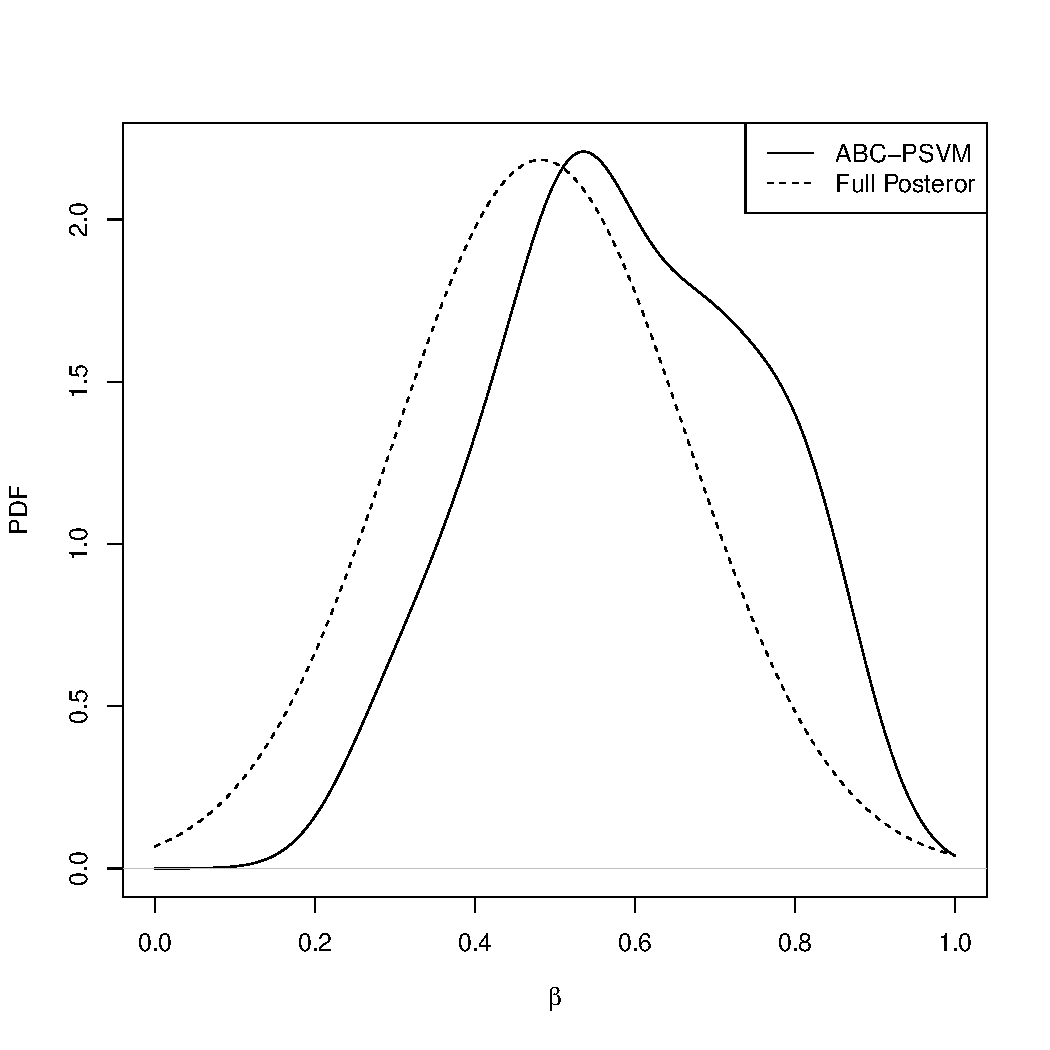
\includegraphics[scale=0.7]{ABCvsFull_100_1000_4.pdf}\protect\caption{ABC Density vs True Posterior Density\label{fig:ABC-vs-True}}
\end{figure}
The slight skewness in Fig. \ref{fig:ABC-vs-True} possibly due the
the small sample size of the observed data. Another interesting result
of this simulation is shown in Fig. \ref{fig:ss-vs-mle}. 
\begin{figure}
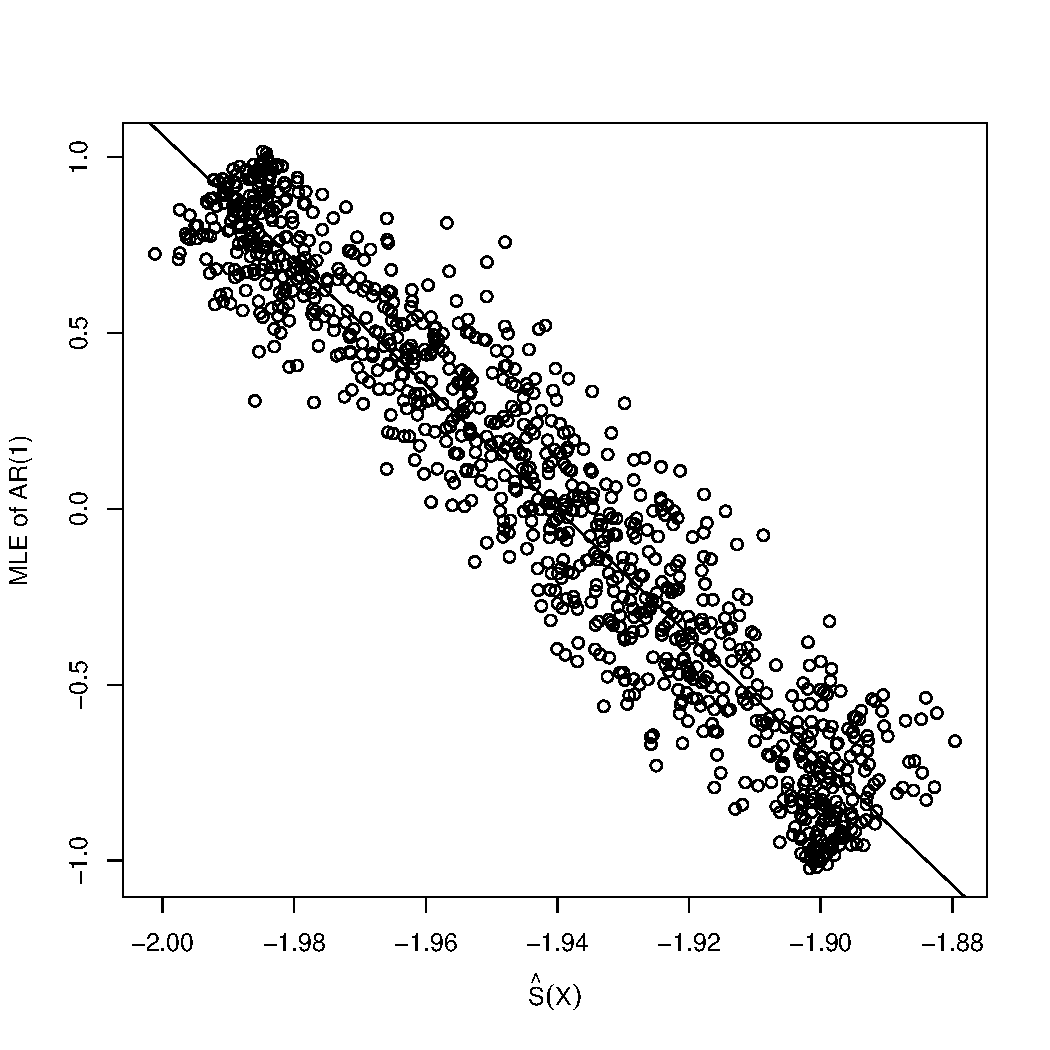
\includegraphics[scale=0.7]{ESSvsMLE_100_1000_4.pdf}\protect\caption{Estimated Summary Statistic vs MLE\label{fig:ss-vs-mle}}
\end{figure}
There is a strong linear relationship between the estimated summary
statistic and MLE 
\[
\hat{\beta}=\frac{\sum_{i=1}^{99}Y_{i}Y_{i+1}}{\sum_{i=1}^{99}Y_{i}^{2}},
\]
which is one of the most efficient summary {{} } {statistics
} based on Theorems \ref{thm:bernstein-von-mises-mle} and \ref{thm:partial-post-m-est}.
Hence, our algorithm will automatically approach the most efficient
summary statistics in a nonparametric way. 
\end{example}

\section{\label{sec:Discussion}Discussion}

\begin{comment}
not know epsilon sufficient, not know sufficient lead to intrinsic
consistency,regression had to generate to multivariate theta,dim must
be same
\end{comment}
In this paper, we explore ABC both from a theoretical and computational
points of view. The theory part architects the foundation of ABC by
linking asymptotic properties of statistics to that of the partial
posterior. The application part innovates the algorithm by virtue
of bridging selection of summary statistics and SDR. However, although
the theory in \citet{li1992principal} is very powerful and may be
used as a theoretical guard of our algorithm, it heavily depends on
the relation (\ref{eq:sdr}) holding rigorously. We do not know whether
the result from principal support vector machine would be defunct
if (\ref{eq:sdr}) is only valid in $\varepsilon$-sufficient way.
Moreover, bringing in dimension reduction regression settings perhaps
moderates the usage when there are multiple parameters of interest,
and may need advance techniques such as envelope models of \citet{su2011partial,su2012inner}. 


\section*{Acknowledgment}

Ghosh's research was partially supported by an NSF Grant.


\appendix
\begingroup 
\let\clearpage\relax 
% command \begingroup \let\clearpage\relax \endgroup shut down the clearpage before \include 
\chapter{Proof for Higher-Order Properties of Bayesian Empirical Likelihood:
Univariate Case}

\section{Behavior Of Log Empirical Likelihood In  The Tail}

The Taylor expansion consists of  expanding the log empirical
likelihood and prior density around the mean and  then control
the tail part of the log empirical likelihood. In order to implement
this idea, the tail part of $\tilde{l}\left(\theta\right)$ must vanish
faster than the required polynomial order. In this section,
we will show that indeed the tail part of $\tilde{l}\left(\theta\right)$
vanishes at an exponential rate.
\begin{lemma}
\label{lemma:exponential-decay-tail} Under  Assumptions 1 and 2, for any $\delta_{1}>0$, there
exist $\varepsilon_{1}>0$ and $N_{3}$, such that 
\[
\tilde{l}\left(\theta\right)-\tilde{l}\left(\tilde{\theta}\right)\le-\varepsilon,\ascv,
\]
for any $\left|b\left(\theta-\tilde{\theta}\right)\right|\ge\delta_{1}$
and $\theta\in H_n$, where $b=\left[\left\{ n^{-1}\sum_{i=1}^{n}\diff g\left(X_{i},\tilde{\theta}\right)/\diff\theta\right\} ^{2}/\left\{ n^{-1}\sum_{i=1}^{n}g\left(X_{i},\tilde{\theta}\right)^{2}\right\} \right]^{-1/2}$\end{lemma}
\begin{proof}
By Lemma 3, we know that $\tilde{\theta}$ is the unique maximizer%
\begin{comment}
need to be assume
\end{comment}
. Therefore, for any $\theta\neq\tilde{\theta}$, $\tilde{l}\left(\theta\right)<\tilde{l}\left(\tilde{\theta}\right)$.
The set 
\[
\left\{ \theta:\left|b\left(\theta-\tilde{\theta}\right)\right|\ge\delta_{1}\right\} \cap H_n
\]
is a compact set, and $\tilde{l}\left(\theta\right)$ is a continuous
function. Hence there exists a $\theta^{*}\in\left\{ \theta:\left|b\left(\theta-\tilde{\theta}\right)\right|\ge\delta_{1}\right\} \cap H_n$
, such that for any $\theta\in\left\{ \theta:\left|b\left(\theta-\tilde{\theta}\right)\right|\ge\delta_{1}\right\} \cap H_n$,
\[
\tilde{l}\left(\theta\right)\le\tilde{l}\left(\theta^{*}\right).
\]
Therefore, $\tilde{l}\left(\theta\right)\le\tilde{l}\left(\theta^{*}\right)<\tilde{l}\left(\tilde{\theta}\right)$, which is equivalent to 
\[
\tilde{l}\left(\theta\right)-\tilde{l}\left(\tilde{\theta}\right)\le\tilde{l}\left(\theta^{*}\right)-\tilde{l}\left(\tilde{\theta}\right)<0.
\]
Let $\varepsilon_{1}=\left\{ \tilde{l}\left(\tilde{\theta}\right)-\tilde{l}\left(\theta^{*}\right)\right\} /2$,
then we have 
\[
\tilde{l}\left(\theta\right)-\tilde{l}\left(\tilde{\theta}\right)\le\tilde{l}\left(\theta^{*}\right)-\tilde{l}\left(\tilde{\theta}\right)<\varepsilon_{1}.
\]

\end{proof}

\section{Higher-Order Derivatives}\label{app:high-order-der}

In order to expand around the mean, we need to control the
remainder terms in the Taylor expansion, which involves the finiteness of higher-order
derivatives of $\tilde{l}$. 
\begin{lemma}
\label{lem:control-higher-order-derivative-l}Let%
\begin{comment}
this lemma need change
\end{comment}
{} 
\[
\omega_{i}\left(\theta\right)=\begin{cases}
\left\{ 1+\nu\left(\theta\right)g\left(X_{i},\theta\right)\right\} ^{-1}, & \mathrm{for\: empirical\: likelihood,}\\
\exp\left\{ -\nu\left(\theta\right)g\left(X_{i},\theta\right)\right\} , & \mathrm{for\: exponentially\: tilted\: empirical\: likelihood,}\\
\left\{ \mu\left(\theta\right)+\nu\left(\theta\right)g\left(X_{i},\theta\right)\right\} ^{-1/\left(\lambda+1\right)}, & \mathrm{for\: Cressie-Read\: empirical\: likelihood.}
\end{cases}
\]
and 
\[
D=\begin{cases}
n^{-1}\sum_{i=1}^{n}\omega_{i}^{r}g\left(X_{i},\theta\right)^{2}, & \mathrm{for\: empirical\: and\: exponentially\:tilted,}\\
n^{-1}\sum_{i=1}^{n}\omega_{i}^{\lambda+2}\left[g\left(X_{i},\theta\right)-\left\{ n^{-1}\sum_{i=1}^{n}\omega_{i}^{\lambda+2}g\left(X_{i},\theta\right)\right\} \right]^{2}, & \mathrm{for\: Cressie-Read.}
\end{cases}
\]
Then  under Assumptions 1 and 3, for any $k=2,\ldots K+3$ , 
\begin{eqnarray*}
\frac{\diff^{k}}{\diff\theta^{k}}\tilde{l}\left(\theta\right) & = & D^{-r_{k}}P_{k}\left(M_{1},M_{2},\ldots,\nu,\mu\right),
\end{eqnarray*}
where $P_{k}$ are polynomial function , and all the $r_{j}<C\left(k\right)$,
and $C\left(k\right)$ is some constant only depending on$k$, and
$M_{j}$ are the weighted average of higher order derivatives of $g$,
i.e. 
\[
M_{j}=\frac{1}{n}\sum_{i=1}^{n}\omega_{i}^{r}\prod_{l}\frac{\diff^{l}g\left(X_{i},\theta\right)}{\diff\theta^{l}},
\]
$l$ can be the same . \end{lemma}
\begin{proof}
From Lemma 2, we know that 
\[
\frac{\diff\nu}{\diff\theta}=D^{-1}P_{1}\left\{ \frac{1}{n}\sum_{i=1}^{n}\omega_{i}^{r_{1}}\frac{\diff g\left(X_{i},\theta\right)}{\diff\theta},\frac{1}{n}\sum_{i=1}^{n}\omega_{i}^{r_{2}}g\left(X_{i},\theta\right),\ldots,\nu,\mu\right\} .
\]
Moreover, 
\begin{eqnarray*}
\frac{\diff\tilde{l}^{\mathrm{EL}}\left(\theta\right)}{\diff\theta} & = & \sum_{i=1}^{n}\frac{1}{1+\nu g\left(X_{i},\theta\right)}\left\{ \frac{\diff\nu}{\diff\theta}g\left(X_{i},\theta\right)+\nu\frac{\diff g\left(X_{i},\theta\right)}{\diff\theta}\right\} \\
 & = & \frac{\diff\nu}{\diff\theta}\frac{1}{n}\sum_{i=1}^{n}\omega_{i}\left(\theta\right)g\left(X_{i},\theta\right)+\nu\frac{1}{n}\sum_{i=1}^{n}\omega_{i}\left(\theta\right)\frac{\diff g\left(X_{i},\theta\right)}{\diff\theta},
\end{eqnarray*}
\[
\frac{\diff\tilde{l}^{\mathrm{ET}}\left(\theta\right)}{\diff\theta}=-\frac{\diff\nu}{\diff\theta}\frac{1}{n}\sum_{i=1}^{n}g\left(X_{i},\theta\right)-\nu\frac{1}{n}\sum_{i=1}^{n}\frac{\diff g\left(X_{i},\theta\right)}{\diff\theta}+\nu\sum_{i=1}^{n}\hat{w}_{i}\left(\theta\right)\frac{\diff g\left(X_{i},\theta\right)}{\diff\theta},
\]
\begin{eqnarray*}
\frac{\diff\tilde{l}^{\mathrm{CR}}\left(\theta\right)}{\diff\theta} & = & -\frac{1}{\lambda+1}\sum_{i=1}^{n}\omega_{i}^{\lambda+1}\left\{ \frac{\diff\mu}{\diff\theta}+\frac{\diff\nu}{\diff\theta}g\left(X_{i},\theta\right)+\nu\frac{\diff g\left(X_{i},\theta\right)}{\diff\theta}\right\} \\
 & = & -\frac{1}{\lambda+1}\left\{ \frac{\diff\mu}{\diff\theta}\frac{1}{n}\sum_{i=1}^{n}\omega_{i}^{\lambda+1}+\frac{\diff\nu}{\diff\theta}\frac{1}{n}\sum_{i=1}^{n}\omega_{i}^{\lambda+1}g\left(X_{i},\theta\right)+\nu\frac{1}{n}\sum_{i=1}^{n}\omega_{i}^{\lambda+1}\frac{\diff g\left(X_{i},\theta\right)}{\diff\theta}\right\} .
\end{eqnarray*}
So for $k=1$, the lemma holds. Assume for $k=n$, the lemma holds. Then 
for $k=n+1$, 
\begin{eqnarray*}
\frac{\diff^{n+1}\tilde{l}\left(\theta\right)}{\diff\theta^{n+1}} & = & \frac{\diff}{\diff\theta_{}}\frac{\diff^{k}\tilde{l}\left(\theta\right)}{\diff\theta}=-r_{k}D^{-r_{k}-1}\left(\frac{\diff D}{\diff\theta}\sum_{i=1}^{k_{n}}\frac{\diff P_{k}}{\diff M_{i}}\frac{\diff M_{i}}{\diff\theta}+\frac{\diff P_{k}}{\diff\nu}\frac{\diff\nu}{\diff\theta}+\frac{\diff P_{k}}{\diff\mu}\frac{\diff\mu}{\diff\theta}\right)
\end{eqnarray*}
The partial derivative of $P_{k}$ is still a polynomial. Also, $D$
itself is a polynomial in $n^{-1}\sum_{i=1}^{n}\omega_{i}^{r}g\left(X_{i},\theta\right)^2$,
$\mu$, and $\nu$. Next 
\begin{eqnarray*}
\frac{\diff M_{i}}{\diff\theta} & = & \frac{1}{n}\sum_{i=1}^{n}\left\{ r\omega_{i}^{r-1}\frac{\diff\omega_{i}}{\diff\theta}\prod_{l}\frac{\diff^{l}g\left(X_{i},\theta\right)}{\diff\theta^{l}}+\omega_{i}^{r}\sum_{l_{j}}\prod_{l\neq l_{j}}\frac{\diff^{l}g\left(X_{i},\theta\right)}{\diff\theta^{l}}\frac{\diff^{l_{j}+1}g\left(X_{i},\theta\right)}{\diff\theta^{l_{j}+1}}\right\} \\
 & = & \frac{r}{n}\sum_{i=1}^{n}\omega_{i}^{r-1}\prod_{l}\frac{\diff^{l}g\left(X_{i},\theta\right)}{\diff\theta^{l}}\frac{\diff\omega_{i}}{\diff\theta}+\sum_{l_{j}}\frac{1}{n}\sum_{i=1}^{n}\omega_{i}^{r}\prod_{l\neq l_{j}}\frac{\diff^{l}g\left(X_{i},\theta\right)}{\diff\theta^{l}}\frac{\diff^{l_{j}+1}g\left(X_{i},\theta\right)}{\diff\theta^{l_{j}+1}}.
\end{eqnarray*}
Similar to the calculation of the first order derivative of empirical
log likelihood, we know the $\diff\omega_{i}/\diff\theta$ are polynomials
involving terms like $M_{i}$. So for $k=n+1$, the higher order derivatives
of empirical log likelihood are of a similar form. Hence, by mathematical
induction, the lemma holds for all $n$. 
\end{proof}
By Lemma \ref{lem:control-higher-order-derivative-l}, the higher-order derivatives of log empirical likelihood are rational functions of the sample moments of higher-order derivatives of  $g$. We can anticipate
that higher order derivatives of log empirical likelihood can be bounded
in a small neighborhood of the true parameter when sample size is
large , provided the population moments of higher-order derivatives of function $g$ are finite. This we prove in the following lemma .


\begin{lemma}
\label{lem:bounded-high-order-der} Under Assumptions 3 , 4 and 5 ,
there exist constants $\delta_{2}$, $C_{3}$ and $N_{4}$ such that
for any $\left|b\left(\theta-\tilde{\theta}\right)\right|\le\delta_{2}$
and $n>N_{4}$, any $j=1,\ldots,k$,%
\begin{comment}
need add consistency conditions for M-Estimator
\end{comment}
{} 
\begin{equation}
\left|\frac{\diff^{j}\tilde{l}\left(\theta\right)}{\diff\theta^{j}}\right|\le C_{3}.\label{eq:bounded-higher-order-derivatives}
\end{equation}
\end{lemma}
\begin{proof}
All $\omega_{i}$ in Lemma \ref{lem:control-higher-order-derivative-l}
are equal to $1$ when evaluated at $\tilde{\theta}$. Under the assumption
of finite moments, by strong law of large numbers, and strong consistency
of the $M$-estimator $\tilde{\theta}$, we have 
\[
M_{j}=\frac{1}{n}\sum_{i=1}^{n}\prod_{l}\frac{\diff^{l}g\left(X_{i},\tilde{\theta}\right)}{\diff\theta^{l}}\rightarrow E\left\{ \prod_{l}\frac{\diff^{l}g\left(X_{1},\theta_{0}\right)}{\diff\theta^{l}}\right\} <\infty,\ascv.
\]
 By Lemma 3, the higher order
derivatives are continuous functions. Hence for any small number $\varepsilon_{2}>0$,
there exists a constant $\delta_{2}$ such that whenever $\left|b\left(\theta-\tilde{\theta}\right)\right|\le\delta_{2}$,
\[
\left|\frac{\diff^{j}\tilde{l}\left(\theta\right)}{\diff\theta^{j}}-\frac{\diff^{j}\tilde{l}\left(\tilde{\theta}\right)}{\diff\theta^{j}}\right|<\varepsilon_{2}.
\]
By Lemma \ref{lem:control-higher-order-derivative-l}, there exists
a constant $N_{4}$, such that whenever $n>N_{4}$. 
\[
\left|\frac{\diff^{j}\tilde{l}\left(\theta\right)}{\diff\theta^{j}}-\frac{P_{k}\left[E\left\{ \prod_{l}\diff^{l}g\left(X_{1},\theta_{0}\right)/\diff\theta^{l}\right\} ,\ldots,0,1\right]}{D^{r_{k}}}\right|<\varepsilon_{2}.
\]
By assumption, all the moments are bounded when $k\le K+3$.
Then there exist a constant $C_{3}$, such that 
\[
D^{-r_{k}}P_{k}\left[E\left\{ \prod_{l}\frac{\diff^{l}g\left(X_{1},\theta_{0}\right)}{\diff\theta^{l}}\right\} ,\ldots,0,1\right]\le C_{3},
\]
 %
\begin{comment}
change the length
\end{comment}
 which leads to (\ref{eq:bounded-higher-order-derivatives}). 
\end{proof}

\section{Expansion Near The M-Estimator}
\begin{lemma}
\label{lem:near-mean-2nd-order-bound-1}.  Under  Assumptions 1 and 2,there exists a $\delta_{3}>0$,
such that 
\[
\sum_{i=1}^{n}\log\hat{w}_{i}\left(\theta\right)-\sum_{i=1}^{n}\log\hat{w}_{i}\left(\tilde{\theta}\right)\le-\frac{1}{4}y^{2},
\]
for any $\theta\in\left\{ \theta:\left|b\left(\theta-\tilde{\theta}\right)\right|<\delta_{3}\right\} \cap H$
. \end{lemma}
\begin{proof}
By Taylor expansion, 
\begin{eqnarray*}
\frac{1}{n}\left\{ \sum_{i=1}^{n}\log\hat{w}_{i}\left(\theta\right)-\sum_{i=1}^{n}\log\hat{w}_{i}\left(\tilde{\theta}\right)\right\}  & = & \frac{\diff\tilde{l}\left(\tilde{\theta}\right)}{\diff\theta}\left(\theta-\tilde{\theta}\right)+\frac{1}{2}\frac{\diff^{2}\tilde{l}\left(\theta^{*}\right)}{\diff\theta^{2}}\left(\theta-\tilde{\theta}\right)^{2},
\end{eqnarray*}
where $\left|\theta^{*}-\tilde{\theta}\right|\le\left|\theta-\tilde{\theta}\right|$.
By Lemma 4, the first term in above equation
is zero. By Lemma \ref{lem:control-higher-order-derivative-l}, we
know that $\diff^{2}\tilde{l}\left(\theta\right)/\diff\theta^{2}$
is a continuous function in $\theta$. Thus there exists a $\delta_{3}$,
such that for any $\left|b\left(\theta^{*}-\tilde{\theta}\right)\right|\le\left|b\left(\theta-\tilde{\theta}\right)\right|<\delta_{3}$,
\[
\left|\frac{\diff^{2}\hat{l}\left(\theta^{*}\right)}{\diff\theta^{2}}\left(\theta-\tilde{\theta}\right)^{2}+\left|b\left(\theta-\tilde{\theta}\right)\right|^{2}\right|<\frac{1}{2}\left|b\left(\theta-\tilde{\theta}\right)\right|^{2}.
\]
Hence $\diff^{2}\tilde{l}\left(\theta^{*}\right)/\diff\theta^{2}\left(\theta-\tilde{\theta}\right)^{2}<-\left|b\left(\theta-\tilde{\theta}\right)\right|^{2}/2$,
 so that, 
\[
\sum_{i=1}^{n}\log\hat{w}_{i}\left(\theta\right)-\sum_{i=1}^{n}\log\hat{w}_{i}\left(\tilde{\theta}\right)<\frac{1}{2}\times\frac{1}{2}\left|\sqrt{n}b\left(\theta-\tilde{\theta}\right)\right|^{2}=\frac{1}{4}y^{2}.
\]
\end{proof}
The next lemma plays a key role in expanding the posterior, and can be interpreted as an empirical likelihood version of the Edgeworth expansion. 
\begin{lemma}
\label{lem:central-expansion-lik} Under  Assumptions 1 , 3 , 4 and 5 , then there exist $\delta_{4}$, $M_{3}$
and $N_{5}$, such that 
\[
\left|\int_{-\sqrt{n}\delta_{4}}^{\sqrt{n}\delta_{4}}\exp\left\{ -\frac{1}{2}y^{2}+\sum_{k=3}^{K+3}a_{kn}\left(\frac{y}{b}\right)^{k}n^{-\left(k-2\right)/2}\right\} -\prod_{i=1}^{n}\frac{\hat{w}_{i}\left(\theta\right)}{\hat{w}_{i}\left(\tilde{\theta}\right)}\diff y\right|\le M_{3}n^{-\left(K+2\right)/2},\:\ascv.
\]
\end{lemma}
\begin{proof}
Let $\delta_{4}\le\min\left(\delta_{2},\delta_{3}\right)$ in Lemma
\ref{lem:bounded-high-order-der} and Lemma \ref{lem:near-mean-2nd-order-bound-1}
\begin{eqnarray*}
 &  & \int_{-\sqrt{n}\delta_{4}}^{\sqrt{n}\delta_{4}}\exp\left\{ -\frac{1}{2}y^{2}+\sum_{k=3}^{K+3}a_{kn}\left(\frac{y}{b}\right)^{k}n^{-\left(k-2\right)/2}\right\} -\prod_{i=1}^{n}\frac{\hat{w}_{i}\left(\theta\right)}{\hat{w}_{i}\left(\tilde{\theta}\right)}\diff y\\
 & = & \int_{-\sqrt{n}\delta_{4}}^{\sqrt{n}\delta_{4}}\exp\left\{ \sum_{i=1}^{n}\log\hat{w}_{i}\left(\theta\right)-\sum_{i=1}^{n}\log\hat{w}_{i}\left(\tilde{\theta}\right)\right\} \\
 &  & \left[\exp\left\{ -\frac{1}{2}y^2+\sum_{k=3}^{K+3}a_{kn}\left(\frac{y}{b}\right)^{k}n^{-\left(k-2\right)/2}-\sum_{i=1}^{n}\log\hat{w}_{i}\left(\theta\right)+\sum_{i=1}^{n}\log\hat{w}_{i}\left(\tilde{\theta}\right)\right\} -1\right]\diff y.
\end{eqnarray*}
By %
Lemma \ref{lem:near-mean-2nd-order-bound-1}, %
Lemma \ref{lem:bounded-high-order-der} and Taylor expansion, the
above equation is bounded by 
\begin{eqnarray}
 &  & \int_{-\sqrt{n}\delta_{4}}^{\sqrt{n}\delta_{4}}\exp\left(-\frac{y^{2}}{4}\right)\left|\exp\left\{ -a_{K+4,n}\left(\theta^{*}\right)\left(\frac{y}{b}\right)^{K+4}n^{-\left(K+2\right)/2}\right\} -1\right|\diff y\nonumber \\
 & \le & \int_{-\sqrt{n}\delta_{4}}^{\sqrt{n}\delta_{4}}\exp\left(-\frac{y^{2}}{4}\right)\left|\exp\left\{ -C_{1}\left(\frac{y}{b}\right)^{K+4}n^{-\left(K+2\right)/2}\right\} -1\right|\diff y.\label{eq:bounded-central-int-likratio}
\end{eqnarray}
where $\left|\theta^{*}-\tilde{\theta}\right|\le\left|\theta-\tilde{\theta}\right|<\delta_{4}$,
and $C_{4}$ is some constant dependent on $\delta_{4}$, $N_{5}$
and $a_{K+4,n}\left(\tilde{\theta}\right)$. For sufficiently large
$n$, and sufficiently small $\delta_{4}$, $a_{K+4,n}\left(\theta^{*}\right)$
is very close to $a_{K+4,n}\left(\tilde{\theta}\right)$, and by %
Lemma \ref{lem:bounded-high-order-der}, $a_{K+4,n}\left(\tilde{\theta}\right)$
is finite. Hence, for very large $n$,  $\exp\left\{ -C_{4}\left(y/b\right)^{K+4}n^{-\left(k+2\right)/2}\right\} -1$
does not change sign on either $\left[-\sqrt{n}\delta_{4},0\right]$
and $\left[0,\sqrt{n}\delta_{4}\right]$. So without loss of generality,
we assume $\exp\left\{ -C_{4}\left(y/b\right)^{K+4}n^{-\left(K+2\right)/2}\right\} -1\ge0$
on $\left[-\sqrt{n}\delta_{4},\sqrt{n}\delta_{4}\right]$. With $t=\sqrt{n}$,%
\begin{comment}
unique the introduction of y
\end{comment}
{} and $t\in\mathbb{R}^{+}$, the last term in (\ref{eq:bounded-central-int-likratio})
can be written as 
\[
\int_{-\delta_{4}t}^{\delta_{4}t}\exp\left(-\frac{y^{2}}{4}\right)\left\{ \exp\left(-\frac{C_{4}}{b^{K+4}}y^{K+4}t^{-K-2}\right)-1\right\} \diff y.
\]
If we can show that 
\[
\lim_{t\rightarrow+\infty}\frac{\int_{-\delta_{4}t}^{\delta_{4}t}\exp\left(-y^{2}/4\right)\left\{ \exp\left(-C_{4}y^{K+4}t^{-K-2}/b^{K+4}\right)-1\right\} \diff y}{t^{-K-2}}=C_{5},
\]
for some $C_{5}<\infty$, the lemma is proved. Take the derivative
with respect to $t$ in both the numerator and the denominator. In the denominator,
$\left(t^{-K-2}\right)'=-\left(K+2\right)t^{-K-3}.$ In the numerator,
\begin{eqnarray}
 &  & \frac{\diff}{\diff t}\int_{-\delta_{4}t}^{\delta_{4}t}\exp\left(-\frac{y^{2}}{4}\right)\left\{ \exp\left(-\frac{C_{4}}{b^{K+4}}y^{K+4}t^{-K-2}\right)-1\right\} \diff y\nonumber \\
 & = & \int_{-\delta_{4}t}^{\delta_{4}t}\exp\left(-\frac{y^{2}}{4}\right)\left(-\frac{C_{4}}{b^{K+4}}y^{K+4}\right)\left(-K-2\right)t^{-K-3}\exp\left(-\frac{C_{4}}{b^{K+4}}y^{K+4}t^{-K-2}\right)\diff y\nonumber \\
 &  & +\exp\left\{ -\frac{\left(\delta_{4}t\right)^{2}}{4}\right\} \left[\exp\left\{ -\frac{C_{4}}{b^{K+4}}\left(\delta_{4}t\right)^{K+4}t^{-K-2}\right\} -1\right]\delta_{4}-\exp\left\{ -\frac{\left(-\delta_{4}t\right)^{2}}{4}\right\} \nonumber \\
 &  & \left[\exp\left\{ -\frac{C_{4}}{b^{K+4}}\left(-\delta_{4}t\right)^{K+4}t^{-K-2}\right\} -1\right]\left(-\delta_{4}\right)\nonumber \\
 & = & \frac{\left(K+2\right)C_{4}}{b^{K+4}}t^{-K-3}\int_{-\delta_{4}t}^{\delta_{4}t}y^{K+4}\exp\left(-\frac{y^{2}}{4}-\frac{C_{4}}{b^{K+4}}y^{K+4}t^{-K-2}\right)\diff y\nonumber \\
 &  & +\delta_{4}\left[\exp\left\{ -\left(\frac{\delta_{4}^{2}}{4}-\frac{C_{4}}{b^{K+4}}\delta_{4}^{K+4}\right)t^{2}\right\} -\exp\left(-\frac{\delta_{4}^{2}t^{2}}{4}\right)\right]\label{eq:lhospital-diff-numerator}\\
 &  & +\delta_{4}\left(\exp\left[-\left\{ \frac{\delta_{4}^{2}}{4}-\frac{C_{1}}{b^{K+4}}\left(-\delta_{4}\right)^{K+4}\right\} t^{2}\right]-\exp\left(-\frac{\delta_{4}^{2}t^{2}}{4}\right)\right).\nonumber 
\end{eqnarray}
We choose $\delta_{4}$ sufficiently small such that 
\begin{equation}
\delta_{4}<\min\left(\sqrt[K+2]{\frac{b^{K+4}}{4\left|C_{4}\right|}},\delta_{2},\delta_{3}\right).\label{eq:choose-delta-2}
\end{equation}
Hence, 
\[
0<\frac{\delta_{4}^{2}}{4}-\frac{\left|C_{4}\right|}{b^{K+4}}\delta_{4}^{K+4}\le\frac{\delta_{4}^{2}}{4}-\frac{C_{4}}{b^{K+4}}\left(\pm\delta_{4}\right)^{K+4},
\]
and 
\[
\lim_{t\rightarrow+\infty}\frac{\delta_{4}\left[\exp\left\{ -\left(\delta_{4}^{2}/4-\left|C_{4}\right|\delta_{2}^{K+4}/b^{K+4}\right)t^{2}\right\} -\exp\left(-\delta_{4}^{2}t^{2}/4\right)\right]}{-\left(K+2\right)t^{-K-3}}=0.
\]
Hence, the last two terms in (\ref{eq:lhospital-diff-numerator})
tend to zero when $t\rightarrow+\infty$. Now we consider the ratio
\begin{eqnarray}
 &  & \frac{\left\{ \left(K+2\right)C_{4}/b^{K+4}\right\} t^{-K-3}\int_{-\delta_{4}t}^{\delta_{4}t}y^{K+4}\exp\left(-y^{2}/4-C_{4}y^{K+4}t^{-K-2}/b^{K+4}\right)\diff y}{-\left(K+2\right)t^{-K-3}}\nonumber \\
 & = & -\frac{C_{4}}{b^{K+4}}\int_{-\delta_{4}t}^{\delta_{4}t}y^{K+4}\exp\left(-\frac{y^{2}}{4}-\frac{C_{4}}{b^{K+4}}y^{K+4}t^{-K-2}\right)\diff y.\label{eq:lhopstal-diff-1st-ratio}
\end{eqnarray}
Since $\delta_{4}$ satisfies (\ref{eq:choose-delta-2}), (\ref{eq:lhopstal-diff-1st-ratio})
is bounded by 
\begin{eqnarray*}
 &  & \frac{\left|C_{4}\right|}{b^{K+4}}\int_{-\delta_{4}t}^{\delta_{4}t}\left|y\right|^{K+4}\exp\left\{ -\frac{y^{2}}{4}-\frac{\left|C_{4}\right|}{b^{K+4}}\left(\delta_{4}t\right)^{K+2}y^{2}t^{-K-2}\right\} \diff y\\
 & = & \frac{\left|C_{4}\right|}{b^{K+4}}\int_{-\delta_{4}t}^{\delta_{4}t}\left|y\right|^{K+4}\exp\left\{ -\left(\frac{\delta_{4}^{2}}{4}-\frac{\left|C_{4}\right|}{b^{K+4}}\delta_{4}^{K+4}\right)y^{2}\right\} \diff y\\
 & \rightarrow & \frac{\left|C_{4}\right|}{b^{K+4}}\sqrt{2\pi\left\{ 2\left(\frac{\delta_{4}^{2}}{4}-\frac{\left|C_{4}\right|}{b^{K+4}}\delta_{4}^{K+4}\right)\right\} ^{-1}}\left\{ 2\left(\frac{\delta_{4}^{2}}{4}-\frac{\left|C_{4}\right|}{b^{K+4}}\delta_{4}^{K+4}\right)\right\} ^{-\left(K+4\right)/2}\\ & &\frac{2^{\left(K+4\right)/2}\Gamma\left\{ \left(K+4+1\right)/2\right\} }{\sqrt{\pi}}<\infty.
\end{eqnarray*}
So by L'Hostiple's rule, we have 
\begin{eqnarray*}
 &  & \lim_{t\rightarrow+\infty}\frac{\int_{-\delta_{4}t}^{\delta_{4}t}\exp\left(-y^{2}/4\right)\left\{ \exp\left(-C_{4}y^{K+4}t^{-K-2}/b^{K+4}\right)-1\right\} \diff y}{t^{-K-2}}\\
 & = & \lim_{t\rightarrow+\infty}\frac{\left[\int_{-\delta_{4}t}^{\delta_{4}t}\exp\left(-y^{2}/4\right)\left\{ \exp\left(-C_{4}y^{K+4}t^{-K-2}/b^{K+4}\right)-1\right\} \diff y\right]'}{\left(t^{-K-2}\right)'}=C_{5}<\infty.
\end{eqnarray*}
\end{proof}
\begin{lemma}
\label{lem:central-expansion-post-prod}%
 Under  Assumptions 1 , 3 , 4 and 5 ,  there exists  $\delta_{4}>0$, and constants
$M_{4}$, $N_{6}$, such that 
\begin{equation}
\left|\int_{-\sqrt{n}\delta_{4}}^{\sqrt{n}\delta_{4}}\left[\exp\left\{ -\frac{1}{2}y^{2}+\sum_{k=3}^{K+3}a_{kn}\left(\frac{y}{b}\right)^{k}n^{-\left(k-2\right)/2}\right\} \rho_{K}\left(\theta\right)-\prod_{i=1}^{n}\frac{\hat{w}_{i}\left(\theta\right)}{\hat{w}_{i}\left(\tilde{\theta}\right)}\rho\left(\theta\right)\right]\diff y\right|\le M_{4}n^{-\frac{1}{2}\left(K+1\right)},\:\ascv.\label{eq:central-exp-post}
\end{equation}
\end{lemma}
\begin{proof}
Use $\delta_{4}$ in Lemma \ref{lem:central-expansion-lik}, and apply
Taylor expansion of $\tilde{l}\left(\theta\right)$ around $\tilde{\theta}$.
Then for any $\tilde{\theta}-\delta_{4}/b\le\theta\le\tilde{\theta}+\delta_{4}/b$,
there exists a $\theta^{*}$ which satisfies $\left|b\left(\theta^{*}-\tilde{\theta}\right)\right|\le\left|b\left(\theta-\tilde{\theta}\right)\right|$.
This leads to 
\begin{eqnarray*}
\tilde{l}\left(\theta\right) & = & \tilde{l}\left(\tilde{\theta}\right)+\frac{\diff\tilde{l}\left(\tilde{\theta}\right)}{\diff\theta}\left(\theta-\tilde{\theta}\right)+\frac{1}{2}\frac{\diff^{2}\tilde{l}\left(\tilde{\theta}\right)}{\diff\theta^{2}}\left(\theta-\tilde{\theta}\right)^{2}+\sum_{k=3}^{K+3}a_{kn}\left(\tilde{\theta}\right)\left(\theta-\tilde{\theta}\right)^{k}\\
 &  & +\frac{1}{\left(K+4\right)!}\frac{\diff^{K+4}}{\diff\theta}\tilde{l}\left(\theta^{*}\right)\left(\theta-\tilde{\theta}\right)^{K+4}\\
 & = & \tilde{l}\left(\tilde{\theta}\right)-\frac{1}{2}y^{2}n^{-1}+\sum_{k=3}^{K+3}a_{kn}\left(\frac{y}{b}\right)^{k}n^{-k/2}+\frac{1}{\left(K+4\right)!}\frac{\diff^{K+4}}{\diff\theta}\tilde{l}\left(\theta^{*}\right)\left(\theta-\tilde{\theta}\right)^{K+4}.
\end{eqnarray*}
Now 
\begin{eqnarray*}
 &  & \left|\exp\left\{ -\frac{1}{2}y^{2}+\sum_{k=3}^{K+3}a_{kn}\left(\frac{y}{b}\right)^{k}n^{-\left(k-2\right)/2}\right\} \rho_{K}\left(\theta\right)-\prod_{i=1}^{n}\frac{\hat{w}_{i}\left(\theta\right)}{\hat{w}_{i}\left(\tilde{\theta}\right)}\rho\left(\theta\right)\right|\\
 &  & \le\left|\exp\left\{ -\frac{1}{2}y^{2}+\sum_{k=3}^{K+3}a_{kn}\left(\frac{y}{b}\right)^{k}n^{-\left(k-2\right)/2}\right\} \rho_{K}\left(\theta\right)-\prod_{i=1}^{n}\frac{\hat{w}_{i}\left(\theta\right)}{\hat{w}_{i}\left(\tilde{\theta}\right)}\rho_{K}\left(\theta\right)\right|\\
 &  & +\left|\prod_{i=1}^{n}\frac{\hat{w}_{i}\left(\theta\right)}{\hat{w}_{i}\left(\tilde{\theta}\right)}\rho_{K}\left(\theta\right)-\prod_{i=1}^{n}\frac{\hat{w}_{i}\left(\theta\right)}{\hat{w}_{i}\left(\tilde{\theta}\right)}\rho\left(\theta\right)\right|\\
 &  & \le\left|\rho_{K}\left(\theta\right)\right|\exp\left\{ n\tilde{l}\left(\theta\right)-n\tilde{l}\left(\tilde{\theta}\right)\right\} \left|\exp\left[n\left\{ \tilde{l}\left(\tilde{\theta}\right)-\frac{1}{2}y^{2}n^{-1}+\sum_{k=3}^{K+3}a_{kn}\left(\frac{y}{b}\right)^{k}n^{-k/2}-\tilde{l}\left(\theta\right)\right\} \right]-1\right|\\
 &  & +\exp\left\{ n\tilde{l}\left(\theta\right)-n\tilde{l}\left(\tilde{\theta}\right)\right\} \left|\rho_{K}\left(\theta\right)-\rho\left(\theta\right)\right|.
\end{eqnarray*}
 By Lemma \ref{lem:central-expansion-lik}, the first term in the
right hand side is bounded by 
\[
\left\{ \max_{\tilde{\theta}-\delta_{4}/b\le\theta\le\tilde{\theta}+\delta_{4}/b}\rho_{K}\left(\theta\right)\right\} M_{3}n^{-\left(K+2\right)/2}.
\]
By Lemma \ref{lem:near-mean-2nd-order-bound-1}, and Taylor expansion
of $\rho\left(\theta\right)$, the second term is bounded by 
\begin{eqnarray*}
 &  & \int_{-\sqrt{n}\delta_{4}}^{\sqrt{n}\delta_{4}}\exp\left(-\frac{y^{2}}{4}\right)\frac{n^{-\left(K+1\right)/2}}{\left(K+1\right)!}\rho^{K+1}\left(\theta^{*}\right)y^{K+1}\diff y\\
 & \le & \frac{1}{\left(K+1\right)!}\left\{ \max_{\tilde{\theta}-\delta_{4}/b\le\theta\le\tilde{\theta}+\delta_{4}/b}\rho^{K+1}\left(\theta^{*}\right)\right\} \left\{ \int_{-\sqrt{n}\delta_{4}}^{\sqrt{n}\delta_{4}}\exp\left(-\frac{y^{2}}{4}\right)y^{\left(K+1\right)/2}\diff y\right\} n^{-\left(K+1\right)/2}\\
 & = & \left[\frac{1}{\left(K+1\right)!}\left\{ \max_{\tilde{\theta}-\delta_{4}/b\le\theta\le\tilde{\theta}+\delta_{4}/b}\rho^{K+1}\left(\theta^{*}\right)\right\} \int_{0}^{\infty}\exp\left(-\frac{y^{2}}{4}\right)y^{\left(K+1\right)/2}\diff y\right]n^{-\left(K+1\right)/2}
\end{eqnarray*}
Hence (\ref{eq:central-exp-post}) holds. %
\begin{comment}
add some constant for the bound of rho
\end{comment}

\end{proof}

\section{Proof Of The Fundamental Theorem For Expansion}\label{app-proof-fun-thm}

We first intuitively derive $P_{K}\left(\xi,n\right)$ %
\begin{comment}
add expansion polynomial
\end{comment}
. First, we expand 
\begin{eqnarray*}
 &  & \exp\left\{ \sum_{k=3}^{K+3}a_{kn}\left(\frac{y}{b}\right)^{k}n^{-\left(k-2\right)/2}\right\} \\
 & = & \sum_{i=0}^{K+1}\frac{1}{i!}\left\{ \sum_{k=3}^{K+3}a_{kn}\left(\frac{y}{b}\right)^{k}n^{-\left(k-2\right)/2}\right\} ^{i}\\
 & = & 1+\sum_{i=1}^{K+1}\frac{1}{i!}\sum_{\sum_{u=3}^{K+3}m_{u,i}=i}\binom{i}{m_{3,i},\ldots,m_{K+3,i}}\prod_{u=3}^{K+3}\left(a_{un}\right)^{m_{u,i}}\left(\frac{y}{b}\right)^{\sum_{u=3}^{K+3}m_{u,i}u}n^{-\left\{ \sum_{u=3}^{K+3}m_{u,i}\left(u-2\right)\right\} /2}.
\end{eqnarray*}
Multiplying the above expression by $\rho_{K}$, 
\begin{eqnarray*}
 &  & \exp\left\{ \sum_{k=3}^{K+3}a_{kn}\left(\frac{y}{b}\right)^{k}n^{-\left(k-2\right)/2}\right\} \rho_{K}\left(\theta\right)\\
 & = & \left[1+\sum_{i=1}^{K+1}\frac{1}{i!}\sum_{\sum_{u=3}^{K+3}m_{u,i}=i}\binom{i}{m_{3,i},\ldots,m_{K+3,i}}\prod_{u=3}^{K+3}\left(a_{un}\right)^{m_{u,i}}\left(\frac{y}{b}\right)^{\sum_{u=3}^{K+3}m_{u,i}u}n^{-\left\{ \sum_{u=3}^{K+3}m_{u,i}\left(u-2\right)\right\} /2}\right]\\
 &  & \times\left\{ \rho\left(\tilde{\theta}\right)+\sum_{j=1}^{K}\frac{1}{j!}\rho^{\left(j\right)}\left(\frac{y}{b}\right)^{j}n^{-j/2}\right\} \\
 & = & \rho\left(\tilde{\theta}\right)+\sum_{j=1}^{K}\frac{1}{j!}\rho^{\left(j\right)}\left(\frac{y}{b}\right)^{j}n^{-j/2}+\rho\left(\tilde{\theta}\right)\sum_{i=1}^{K+1}\frac{1}{i!}\\
 &  & \sum_{\sum_{u=3}^{K+3}m_{u,i}=i}\binom{i}{m_{3,i},\ldots,m_{K+3,i}}\prod_{u=3}^{K+3}\left(a_{un}\right)^{m_{u,i}}\left(\frac{y}{b}\right)^{\sum_{u=3}^{K+3}m_{u,i}u}n^{-\left\{ \sum_{u=3}^{K+3}m_{u,i}\left(u-2\right)\right\} /2}\\
 &  & +\left[\sum_{i=1}^{K+1}\frac{1}{i!}\sum_{\sum_{u=3}^{K+3}m_{u,i}=i}\binom{i}{m_{3,i},\ldots,m_{K+3,i}}\prod_{u=3}^{K+3}\left(a_{un}\right)^{m_{u,i}}\left(\frac{y}{b}\right)^{\sum_{u=3}^{K+3}m_{u,i}u}n^{-\left\{ \sum_{u=3}^{K+3}m_{u,i}\left(u-2\right)\right\} /2}\right]\\
 &  & \times\sum_{j=1}^{K}\frac{1}{j!}\rho^{\left(j\right)}\left(\frac{y}{b}\right)^{j}n^{-j/2}.
\end{eqnarray*}
For the third term in the right hand side of the above equation, we
change the summation index. Let $\sum_{u=3}^{K+3}m_{u,i}\left(u-2\right)=h$.
For any $\sum_{u=3}^{K+3}m_{u,i}=i$, $i\le h\le i\left(K+1\right)$,
$h/\left(K+1\right)\le i\le h$. Thus the third term in the summation can
be rearranged as 
\[
\sum_{h=1}^{\left(K+1\right)^{2}}\left\{ \rho\left(\tilde{\theta}\right)\sum_{i=\left\lceil h/\left(K+1\right)\right\rceil }^{h}\frac{1}{i!}\sum_{I_{i,h}}\binom{i}{m_{3,i},\ldots,m_{K+3,i}}\prod_{u=3}^{K+3}\left(a_{un}\right)^{m_{u,i}}\left(\frac{y}{b}\right)^{\sum_{u=3}^{K+3}m_{u,i}u}\right\} n^{-h/2}.
\]
Similarly for the fourth term, let $\sum_{u=3}^{K+3}m_{u,i}\left(u-2\right)+j=h$.
Then the summation can be rearranged as 
\[
\sum_{h=2}^{\left(K+1\right)^{2}+K}\left\{ \sum_{j=1}^{h-1}\frac{1}{j!}\rho^{\left(j\right)}\left(\frac{y}{b}\right)^{j}\sum_{i=\lceil \left(h-j\right)/\left(K+1\right) \rceil}^{h-j}\frac{1}{i!}\sum_{I_{i,h-j}}\binom{i}{m_{3,i},\ldots,m_{K+3,i}}\prod_{u=3}^{K+3}\left(a_{un}\right)^{m_{u,i}}\left(\frac{y}{b}\right)^{\sum_{u=3}^{K+3}m_{u,i}u}\right\} n^{-h/2}.
\]
We collect  same order terms of $n$, and denote the summation of
all the terms with order higher than $K$ to be $R_{K}\left(Y\right)$.
Then we get the product as 
\begin{eqnarray*}
 &  & \rho\left(\tilde{\theta}\right)+\left\{ \rho'\left(\frac{y}{b}\right)+\rho\left(\tilde{\theta}\right)a_{3n}\left(\frac{y}{b}\right)^{3}\right\} n^{-1/2}\\
 &  & +\sum_{h=2}^{K}\Bigg\{ \frac{1}{h!}\rho^{\left(h\right)}\left(\frac{y}{b}\right)^{h}+\sum_{j=0}^{h-1}\frac{1}{j!}\rho^{\left(j\right)}\left(\frac{y}{b}\right)^{j}\\
 &&\times\sum_{i=\left\lceil \left(h-j\right)/\left(K+1\right)\right\rceil }^{h-j}\frac{1}{i!}\sum_{I_{i,h-j}}\binom{i}{m_{3,i},\ldots,m_{K+3,i}}\prod_{u=3}^{K+3}\left(a_{un}\right)^{m_{u,i}}\left(\frac{y}{b}\right)^{\sum_{u=3}^{K+3}m_{u,i}u}\Bigg\} n^{-h/2}+R_{K}\left(y\right).
\end{eqnarray*}
 Integrating any Borel set $\left(Y_{\left(1\right)},\xi\right]$%
\begin{comment}
change into x1 to xi
\end{comment}
, we get the polynomial $P_{K}\left(\xi,n\right)$. Now we prove Theorem
1.%


. 
\begin{proof}
Let $A_{1}=\left\{ \left|y\right|\ge\delta_{4}\sqrt{n}\right\} \cap\left(Y_{\left(1\right)},\xi\right)$
and $A_{2}=\left\{ \left|y\right|<\delta_{4}\sqrt{n}\right\} \cap\left(Y_{\left(1\right)},\xi\right)$,
where $\delta_{4}$ is in Lemma \ref{lem:central-expansion-post-prod}.
Then 
\begin{eqnarray*}
 &  & \left|\int_{Y_{\left(1\right)}}^{\xi}\prod_{i=1}^{n}\frac{\hat{w}_{i}\left(\tilde{\theta}+y/\sqrt{n}b\right)}{\hat{w}_{i}\left(\tilde{\theta}\right)}\rho\left(\tilde{\theta}+\frac{y}{\sqrt{n}b}\right)\diff y-P_{K}\left(\xi,n\right)\right|\\
 & = & \left|\int_{Y_{\left(1\right)}}^{\xi}\left\{ \prod_{i=1}^{n}\frac{\hat{w}_{i}\left(\tilde{\theta}+y/\sqrt{n}b\right)}{\hat{w}_{i}\left(\tilde{\theta}\right)}\rho\left(\tilde{\theta}+\frac{y}{\sqrt{n}b}\right)-\exp\left(-\frac{y^{2}}{2}\right)\sum_{h=0}^{K}\alpha_{h}\left(y,n\right)n^{-h/2}\right\} \diff y\right|\\
 & \le & \left|\int_{A_{1}}\left\{ \prod_{i=1}^{n}\frac{\hat{w}_{i}\left(\tilde{\theta}+y/\sqrt{n}b\right)}{\hat{w}_{i}\left(\tilde{\theta}\right)}\rho\left(\tilde{\theta}+\frac{y}{\sqrt{n}b}\right)-\exp\left(-\frac{y^{2}}{2}\right)\sum_{h=0}^{K}\alpha_{h}\left(y,n\right)n^{-h/2}\right\} \diff y\right|\\
 &  & +\left|\int_{A_{2}}\left\{ \prod_{i=1}^{n}\frac{\hat{w}_{i}\left(\tilde{\theta}+y/\sqrt{n}b\right)}{\hat{w}_{i}\left(\tilde{\theta}\right)}\rho\left(\tilde{\theta}+\frac{y}{\sqrt{n}b}\right)-\exp\left(-\frac{y^{2}}{2}\right)\sum_{h=0}^{K}\alpha_{h}\left(y,n\right)n^{-h/2}\right\} \diff y\right|.
\end{eqnarray*}


For the first term%
, by Lemma \ref{lemma:exponential-decay-tail}, we have
\begin{eqnarray*}
 &  & \left|\int_{A_{1}}\prod_{i=1}^{n}\frac{\hat{w}_{i}\left(\tilde{\theta}+y/\sqrt{n}b\right)}{\hat{w}_{i}\left(\tilde{\theta}\right)}\rho\left(\tilde{\theta}+\frac{y}{\sqrt{n}b}\right)-\exp\left(-\frac{y^{2}}{2}\right)\sum_{h=0}^{K}\alpha_{h}\left(y,n\right)n^{-h/2}\diff y\right|\\
 & \le & \int_{A_{1}}\exp\left\{ n\hat{l}\left(\tilde{\theta}+\frac{y}{\sqrt{n}b}\right)-n\hat{l}\left(\tilde{\theta}\right)\right\} \rho\left(\tilde{\theta}+\frac{y}{\sqrt{n}b}\right)\diff y\\
 &  & +\left|\int_{A_{1}}\exp\left(-\frac{y^{2}}{4}\right)\sum_{h=0}^{K}\alpha_{h}\left(y,n\right)n^{-h/2}\diff y\right|\\
 & \le & \exp\left(-n\varepsilon\right)\int_{A_{1}}\rho\left(\tilde{\theta}+\frac{y}{\sqrt{n}b}\right)\diff y\\
 &  & +\exp\left(-\frac{\delta_{4}^{2}n}{4}\right)\left|\int_{A_{1}}\exp\left(-\frac{y^{2}}{4}\right)\sum_{h=0}^{K}\alpha_{h}\left(y,n\right)n^{-h/2}\diff y\right|\\
 & \le & \exp\left(-n\varepsilon\right)\int_{\mathbb{R}}\rho\left(\tilde{\theta}+\frac{y}{\sqrt{n}b}\right)\diff y+\exp\left(-n\frac{\delta_{4}^{2}}{4}\right)\sum_{h=0}^{K}\left\{ \int_{Y_{\left(1\right)}}^{Y_{\left(n\right)}}\exp\left(-\frac{y^{2}}{4}\right)\left|\alpha_{h}\left(y,n\right)\right|\diff y\right\} n^{-h/2}.
\end{eqnarray*}
The above terms are exponentially decreasing with respect to $n$.
Hence there exist  $N_{1}$, and $M_{5}$, such that for any $n\ge N_{1}$,
\[
\left|\int_{A_{1}}\prod_{i=1}^{n}\frac{\hat{w}_{i}\left(\tilde{\theta}+y/\sqrt{n}b\right)}{\hat{w}_{i}\left(\tilde{\theta}\right)}\rho\left(\tilde{\theta}+\frac{y}{\sqrt{n}b}\right)-\exp\left(-\frac{y^{2}}{2}\right)\sum_{h=0}^{K}\alpha_{h}\left(y,n\right)n^{-h/2}\diff y\right|\le M_{5}n^{-\left(K+1\right)/2}.
\]


For the second term, by Lemma \ref{lem:central-expansion-post-prod},
we have 
\begin{eqnarray*}
 &  & \left|\int_{A_{2}}\prod_{i=1}^{n}\frac{\hat{w}_{i}\left(\tilde{\theta}+y/\sqrt{n}b\right)}{\hat{w}_{i}\left(\tilde{\theta}\right)}\rho\left(\tilde{\theta}+\frac{y}{\sqrt{n}b}\right)-\exp\left(-\frac{y^{2}}{2}\right)\sum_{h=0}^{K}\alpha_{h}\left(y,n\right)n^{-h/2}\diff y\right|\\
 & \le & \left|\int_{A_{2}}\prod_{i=1}^{n}\frac{\hat{w}_{i}\left(\tilde{\theta}+y/\sqrt{n}b\right)}{\hat{w}_{i}\left(\tilde{\theta}\right)}\rho\left(\tilde{\theta}+\frac{y}{\sqrt{n}b}\right)-\exp\left\{ -\frac{1}{2}y^{2}+\sum_{k=3}^{K+3}a_{kn}\left(\tilde{\theta}\right)\left(\frac{y}{b}\right)^{k}n^{-\left(K-2\right)/2}\right\} \rho_{K}\left(\theta\right)\diff y\right|\\
 &  & +\Bigg|\int_{A_{2}}\exp\left\{ -\frac{1}{2}y^{2}+\sum_{k=3}^{K+3}a_{kn}\left(\tilde{\theta}\right)\left(\frac{y}{b}\right)^{k}n^{-\left(K-2\right)/2}\right\} \rho_{K}\left(\tilde{\theta}+\frac{y}{\sqrt{n}b}\right)\\
 & & -\exp\left(-\frac{y^{2}}{2}\right)\sum_{h=0}^{K}\alpha_{h}\left(y,n\right)n^{-h/2}\diff y\Bigg|\\
 & \le & M_{4}n^{-\left(K+1\right)/2}\\
 &  & +\Bigg|\int_{A_{2}}\exp\left\{ -\frac{1}{2}y^{2}+\sum_{k=3}^{K+3}a_{kn}\left(\tilde{\theta}\right)\left(\frac{y}{b}\right)^{k}n^{-\left(K-2\right)/2}\right\} \rho_{K}\left(\tilde{\theta}+\frac{y}{\sqrt{n}b}\right)\\
 & &-\exp\left(-\frac{y^{2}}{2}\right)\sum_{h=0}^{K}\alpha_{h}\left(y,n\right)n^{-h/2}\diff y\Bigg|.
\end{eqnarray*}
For the second term in the right hand side, we add and subtract $R_{K}\left(y\right)$
in integrand, and by Taylor expansion, 
\begin{eqnarray*}
 &  & \left|\int_{A_{2}}\exp\left\{ -\frac{1}{2}y^{2}+\sum_{k=3}^{K+3}a_{kn}\left(\tilde{\theta}\right)\left(\frac{y}{b}\right)^{k}n^{-\left(K-2\right)/2}\right\} \rho_{K}\left(\tilde{\theta}+\frac{y}{\sqrt{n}b}\right)-\exp\left(-\frac{y^{2}}{2}\right)\sum_{h=0}^{K}\alpha_{h}\left(y,n\right)n^{-h/2}\diff y\right|\\
 & \le & \left|\int_{A_{2}}\exp\left(-\frac{y^{2}}{2}\right)\rho_{K}\left(\theta\right)\left[\exp\left\{ \sum_{k=3}^{K+3}a_{kn}\left(\tilde{\theta}\right)\left(\frac{y}{b}\right)^{k}n^{-\left(K-2\right)/2}\right\} -\sum_{i=0}^{K+1}\frac{1}{i!}\left\{ \sum_{k=3}^{K+3}a_{kn}\left(\tilde{\theta}\right)\left(\frac{y}{b}\right)^{k}n^{-\left(K-2\right)/2}\right\} ^{i}\right]\diff y\right|\\
 &  & +\left|\int_{A_{2}}\exp\left(-\frac{y^{2}}{2}\right)R_{K}\left(y\right)\diff n^{-1/2}y\right|\\
 & = & \left|\int_{A_{2}}\exp\left(-\frac{y^{2}}{2}\right)\rho_{K}\left(\theta\right)\frac{1}{\left(K+2\right)!}\exp\left(L\right)\left\{ \sum_{k=3}^{K+3}a_{kn}\left(\tilde{\theta}\right)\left(\frac{y}{b}\right)^{k}n^{-\left(K-2\right)/2}\right\} ^{K+2}\diff y\right|\\
 &  & +\left|\int_{A_{2}}\exp\left(-\frac{y^{2}}{2}\right)R_{K}\left(y\right)\diff y\right|,
\end{eqnarray*}
where $\left|L\right|\le\left|\sum_{k=3}^{K+3}a_{kn}\left(\tilde{\theta}\right)\left(y/b\right)^{k}n^{-\left(K-2\right)/2}\right|$.
We know that $R_{K}\left(y\right)$ is a polynomial with order $n^{-\left(K+1\right)/2}$.
So there exists an $M_{6}$, such that 
\[
\left|\int_{A_{2}}\exp\left(-\frac{y^{2}}{2}\right)R_{K}\left(y\right)\diff y\right|\le M_{6}n^{-\left(K+1\right)/2}.
\]
For the first term, 

\begin{eqnarray}
 &  & \left|\int_{A_{2}}\exp\left(-\frac{y^{2}}{2}\right)\rho_{K}\left(\theta\right)\frac{1}{\left(K+2\right)!}\exp\left(L\right)\left\{ \sum_{k=3}^{K+3}a_{kn}\left(\tilde{\theta}\right)\left(\frac{y}{b}\right)^{k}n^{-\left(K-2\right)/2}\right\} ^{K+2}\diff n^{-1/2}Y\right|\label{eq:1}\\
 & \le & \frac{1}{\left(K+2\right)!}\left|\int_{A_{2}}\exp\left(-\frac{y^{2}}{2}\right)\rho_{K}\left(\theta\right)\exp\left\{ \left|\sum_{k=3}^{K+3}a_{kn}\left(\tilde{\theta}\right)\left(\frac{y}{b}\right)^{k}n^{-\left(K-2\right)/2}\right|\right\} \left\{ \sum_{k=3}^{K+3}a_{kn}\left(\tilde{\theta}\right)\left(\frac{y}{b}\right)^{k}n^{-\left(K-2\right)/2}\right\} ^{K+2}\diff y\right|\nonumber \\
 & = & \frac{1}{\left(K+2\right)!}\Bigg|\int_{A_{2}}\rho_{K}\left(\theta\right)\exp\left\{ -\frac{y^{2}}{2}+\left|\sum_{k=3}^{K+3}a_{kn}\left(\tilde{\theta}\right)\left(\frac{y}{b}\right)^{k}n^{-\left(K-2\right)/2}\right|\right\} \nonumber \\
 &  & \left\{ \sum_{k=3}^{K+3}a_{kn}\left(\tilde{\theta}\right)\left(\frac{y}{b}\right)^{k}n^{-\left(K-2\right)/2}\right\} ^{K+2}\diff y\Bigg|.\nonumber 
\end{eqnarray}
We need $\delta_{4}$ sufficiently small, so that there exist $C_{6}$
and $C_{7}$, such that 
\begin{eqnarray*}
\frac{y^{2}}{2}-\left|\sum_{k=3}^{K+3}a_{kn}\left(\tilde{\theta}\right)\left(\frac{y}{b}\right)^{k}n^{-\left(K-2\right)/2}\right| & \ge & C_{6}y^{2},\\
\sum_{k=3}^{K+3}a_{kn}\left(\tilde{\theta}\right)\left(\frac{y}{b}\right)^{k}n^{-\left(K-2\right)/2} & \le & C_{7}y^{3}n^{-1/2}.
\end{eqnarray*}
 Hence, (\ref{eq:1}) is bounded by 
\begin{eqnarray*}
 &  & \frac{n^{K+2}}{\left(K+2\right)!}\left|\int_{A_{n}}\exp\left(-C_{6}y^{2}\right)\left(C_{7}y^{3}n^{-1/2}\right)^{K+2}\diff y\right|\\
 & \le & \frac{C_{7}^{K+2}}{\left(K+2\right)!}\left|\int_{Y_{\left(1\right)}}^{Y_{\left(n\right)}}\exp\left(-C_{6}y^{2}\right)y^{3\left(K+2\right)}n^{-\left(K+2\right)/2}\diff y\right|\\
 & \le & \frac{C_{7}^{K+2}}{\left(K+2\right)!}\left|\int_{Y_{\left(1\right)}}^{Y_{\left(n\right)}}\exp\left(-C_{6}y^{2}\right)y^{3\left(K+2\right)}\diff y\right|n^{-\left(K+2\right)/2}.
\end{eqnarray*}
Adding all the parts , we get the inequality in Theorem 1
\begin{comment}
add ref to main theorem
\end{comment}
.
\end{proof}


\endgroup

\chapter{Proof for Higher-Order Properties of Bayesian Empirical Likelihood:
Multivariate Case}
\section{Proof of the Lemma 6}
\begin{proof}
First, we prove the lemma for the empirical likelihood.
	\begin{eqnarray*}
\frac{\partial\tilde{l}}{\partial\theta_{k}} & = & \frac{\partial}{\partial\theta_{k}}\frac{1}{n}\sum_{i=1}^{n}\log\frac{1}{n\left(1+\nu^{T}g\left(X_{i},\theta\right)\right)}\\
 & = & -\frac{1}{n}\sum_{i=1}^{n}\frac{{\partial\nu^{T}} / {\partial\theta_{k}}g\left(X_{i},\theta\right)+\nu^{T}{\partial g\left(X_{i},\theta\right)} / {\partial\theta_{k}}}{1+\nu^{T}g\left(X_{i},\theta\right)}\\
 & = & -\frac{\partial\nu^{T}}{\partial\theta_{k}}\sum_{i=1}^{n}\frac{g\left(X_{i},\theta\right)}{n\left(1+\nu^{T}g\left(X_{i},\theta\right)\right)}-\nu^{T}\sum_{i=1}^{n}\frac{{\partial g\left(X_{i},\theta\right)} / {\partial\theta_{k}}}{n\left(1+\nu^{T}g\left(X_{i},\theta\right)\right)}\\
 & = & -\nu^{T}\sum_{i=1}^{n}\frac{{\partial g\left(X_{i},\theta\right)} / {\partial\theta_{k}}}{n\left(1+\nu^{T}g\left(X_{i},\theta\right)\right)}.
\end{eqnarray*}
\begin{eqnarray*}
\frac{\partial^{2}\hat{l}}{\partial\theta_{j}\partial\theta_{k}} & = & -\frac{\partial\nu^{T}}{\partial\theta_{j}}\sum_{i=1}^{n}\frac{{\partial g\left(X_{i},\theta\right)} / {\partial\theta_{k}}}{n\left(1+\nu^{T}g\left(X_{i},\theta\right)\right)}\\
 &  & -\nu^{T}\frac{1}{n}\sum_{i=1}^{n}-\frac{{\partial^{2}g\left(X_{i},\theta\right)} / {\partial\theta_{j}\partial\theta_{k}}\left(1+\nu^{T}g\left(X_{i},\theta\right)\right) }{\left(1+\nu^{T}g\left(X_{i},\theta\right)\right)^{2}}\\
 & & +\nu^T \frac{1}{n}\sum_{i=1}^{n} \frac{{\partial g\left(X_{i},\theta\right)} / {\partial\theta_{k}}\left({\partial\nu^{T}} / {\partial\theta_{j}}g\left(X_{i},\theta\right)+\nu^{T}{\partial g\left(X_{i},\theta\right)} / {\partial\theta_{j}}\right)}{\left(1+\nu^{T}g\left(X_{i},\theta\right)\right)^{2}}.
\end{eqnarray*}

Let $g_{i}=\left(g_{j}\left(X_{i},\theta\right)\right)$, $\nabla g_{i}=\left({\partial g_{j}\left(X_{i},\theta\right)} / {\partial\theta_{k}}\right)$. By (\ref{eq:decreasing-theta-to-nu-2}), 

\begin{eqnarray*}
\frac{\partial\tilde{l}\left(\tilde{\theta}\right)}{\partial\theta\partial\theta^{T}}&=&-\frac{1}{n}\left\{ \sum_{i=1}^{n}\omega_{i}\frac{\partial g\left(X_{i},\tilde{\theta}\right)}{\partial\theta}-\nu^{T}\sum_{i=1}^{n}\omega_{i}^{2}g\left(X_{i},\tilde{\theta}\right)\frac{\partial g\left(X_{i},\tilde{\theta}\right)}{\partial\theta}\right\} ^{T}\left\{ \sum_{i=1}^{n}\omega_{i}^{2}g\left(X_{i},\tilde{\theta}\right)g^{T}\left(X_{i},\tilde{\theta}\right)\right\} \\&&\left\{ \sum_{i=1}^{n}\omega_{i}\frac{\partial g\left(X_{i},\tilde{\theta}\right)}{\partial\theta}-\nu^{T}\sum_{i=1}^{n}\omega_{i}^{2}g\left(X_{i},\tilde{\theta}\right)\frac{\partial g\left(X_{i},\tilde{\theta}\right)}{\partial\theta}\right\} -\frac{\nu^{T}}{n}\sum_{i=1}^{n}\omega_{i}\frac{\partial^{2}g\left(X_{i},\tilde{\theta}\right)}{\partial\theta\partial\theta^{T}}\\&&+\frac{1}{n}\sum_{i=1}^{n}\omega_{i}^{2}\left\{ \nu^{T}\frac{\partial g\left(X_{i},\tilde{\theta}\right)}{\partial\theta}\right\} \left\{ \nu^{T}\frac{\partial g\left(X_{i},\tilde{\theta}\right)}{\partial\theta}\right\} ^{T}.
\end{eqnarray*}
By a similar argument as Lemma \ref{lem:finite-empirical-weight-moment}, we find 
\[
   \lim_{n\rightarrow\infty} \frac{\partial\tilde{l}\left(\tilde{\theta}\right)}{\partial\theta\partial\theta^{T}} = -\left\{E\nabla g (X,\theta_0) \right\}^T \left[E\left\{g (X,\theta_0)g^T (X,\theta_0)\right\}\right]^{-1} \left\{E\nabla g (X,\theta_0)\right\},
\]
and the limit is negative Godambe information matrix, which is negative definite. Hence, there exists an $N$, such that for sufficient large $n\ge N$, ${\partial\tilde{l}\left(\tilde{\theta}\right)} / {\partial\theta\partial\theta^{T}}$ is negative definite.

	Next, we prove the lemma for the exponentially tilted empirical likelihood.
	\begin{eqnarray*}
		\frac{\partial\tilde{l}\left(\theta\right)}{\partial\theta}	&=&	\frac{\partial}{\partial\theta} \left( \sum_{i=1}^{n}-\nu^{T}g\left(X_{i},\theta\right)-n\log\left[\sum_{j=1}^{n}\exp\left\{ -\nu^{T}g\left(X_{j},\theta\right)\right\} \right] \right) \\
	&=&	-\sum_{i=1}^{n}\left\{ \frac{\partial\nu^{T}}{\partial\theta}g\left(X_{i},\theta\right)+\nu^{T}\frac{\partial g\left(X_{i},\theta\right)}{\partial\theta}\right\} \\
	&	&+n\frac{\sum_{j=1}^{n}\exp\left\{- \nu^{T}g\left(X_{j},\theta\right)\right\} \left\{ \partial\nu^{T}/\partial\theta g\left(X_{j},\theta\right)+\nu^{T}\partial g\left(X_{j},\theta\right)/\partial\theta\right\} }{\sum_{j=1}^{n}\exp\left\{ - \nu^{T}g\left(X_{j},\theta\right)\right\} }\\
	&=&	-\frac{\partial\nu^{T}}{\partial\theta}\sum_{i=1}^{n}g\left(X_{i},\theta\right)-\nu^{T}\sum_{i=1}^{n}\frac{\partial g\left(X_{i},\theta\right)}{\partial\theta}+n\sum_{j=1}^{n}\hat{w}_{i}\left(\theta\right)\left\{ \frac{\partial\nu^{T}}{\partial\theta}g\left(X_{j},\theta\right)+\nu^{T}\frac{\partial g\left(X_{j},\theta\right)}{\partial\theta}\right\}\\ 
	&=&	-\frac{\partial\nu^{T}}{\partial\theta}\sum_{i=1}^{n}g\left(X_{i},\theta\right)-\nu^{T}\sum_{i=1}^{n}\frac{\partial g\left(X_{i},\theta\right)}{\partial\theta}+n\nu^{T}\sum_{j=1}^{n}\hat{w}_{i}\left(\theta\right)\frac{\partial g\left(X_{j},\theta\right)}{\partial\theta}
	\end{eqnarray*}
	Using the similar argument as the empirical likelihood case, we have also,
	\[
\lim_{n\rightarrow\infty} \frac{\partial\tilde{l}\left(\tilde{\theta}\right)}{\partial\theta\partial\theta^{T}} = -\left\{E\nabla g (X,\theta_0) \right\}^T \left[E\left\{g (X,\theta_0)g^T (X,\theta_0)\right\}\right]^{-1} \left\{E\nabla g (X,\theta_0)\right\},.
\]
	By the similar calculation, we can find that the Hessian matrix of the Cressie-Read empirical likelihood is positive definite too.
	
\end{proof}
\section{Behavior Of Log Empirical Likelihood In  The Tail}

The Taylor expansion consists of  expanding the log empirical
likelihood and prior density around the mean and  then control
the tail part of the log empirical likelihood. In order to implement
this idea, the tail part of $\tilde{l}\left(\theta\right)$ must vanish
faster than the required polynomial order. In this section,
we will show that indeed the tail part of $\tilde{l}\left(\theta\right)$
vanishes at an exponential rate.
\begin{lemma}
\label{lemma:exponential-decay-tail-2} For any $\delta_{1}>0$, there
exist $\varepsilon_{1}>0$ and $N_{3}$, such that 
\[
\tilde{l}\left(\theta\right)-\tilde{l}\left(\tilde{\theta}\right)\le-\varepsilon,\ascv,
\]
for any $\left|B^T\left(\theta-\tilde{\theta}\right)\right|\ge\delta_{1}$
and $\theta\in H_n$, 
where $B$ is the Cholesky decomposition of
 $\left\{ n^{-1}\sum_{i=1}^{n}\partial g\left(X_{i},\tilde{\theta}\right)/\partial\theta\right\} ^{2}/\left\{ n^{-1}\sum_{i=1}^{n}g\left(X_{i},\tilde{\theta}\right)^{2}\right\} $
 \end{lemma}
\begin{proof}
By Assumption 6, we know that $\tilde{\theta}$ is the unique maximizer%

. Therefore, for any $\theta\neq\tilde{\theta}$, $\tilde{l}\left(\theta\right)<\tilde{l}\left(\tilde{\theta}\right)$.
The set 
\[
\left\{ \theta:\left|B^T\left(\theta-\tilde{\theta}\right)\right|\ge\delta_{1}\right\} \cap H_n
\]
is a compact set, and $\tilde{l}\left(\theta\right)$ is a continuous
function. Hence there exists a $\theta^{*}\in\left\{ \theta:\left|B^T\left(\theta-\tilde{\theta}\right)\right|\ge\delta_{1}\right\} \cap H_n$
, such that for any $\theta\in\left\{ \theta:\left|B^T\left(\theta-\tilde{\theta}\right)\right|\ge\delta_{1}\right\} \cap H_n$,
\[
\tilde{l}\left(\theta\right)\le\tilde{l}\left(\theta^{*}\right).
\]
Therefore, $\tilde{l}\left(\theta\right)\le\tilde{l}\left(\theta^{*}\right)<\tilde{l}\left(\tilde{\theta}\right)$, which is equivalent to 
\[
\tilde{l}\left(\theta\right)-\tilde{l}\left(\tilde{\theta}\right)\le\tilde{l}\left(\theta^{*}\right)-\tilde{l}\left(\tilde{\theta}\right)<0.
\]
Let $\varepsilon_{1}=\left\{ \tilde{l}\left(\tilde{\theta}\right)-\tilde{l}\left(\theta^{*}\right)\right\} /2$,
then we have 
\[
\tilde{l}\left(\theta\right)-\tilde{l}\left(\tilde{\theta}\right)\le\tilde{l}\left(\theta^{*}\right)-\tilde{l}\left(\tilde{\theta}\right)<\varepsilon_{1}.
\]

\end{proof}

\section{Higher-Order Derivatives}\label{app:high-order-der}

In order to expand around the mean, we need to control the
remainder terms in the Taylor expansion, which involves the finiteness of higher-order
derivatives of $\tilde{l}$. 
\begin{lemma}
\label{lem:control-higher-order-derivative-2}
For any $k=1,2,\ldots,$ $\left(u_{1},u_{2},\ldots,u_{k}\right)\subset\left\{ 1,2,\ldots,p\right\} $,
where some of $u_{i}$s can be equal. Let 
\[
D=\begin{cases}
\left|n^{-1}G^{T}\mathrm{diag}\left(\omega_{1}^{r},\omega_{2}^{r},\ldots,\omega_{n}^{r}\right)G\right|, & \text{for EL or ETEL,}\\
\left|n^{-1}\left(\begin{array}{cc}
G^{T}\mathrm{diag}\left(q_{1},\ldots,q_{n}\right)G & \left(q_{1},\ldots,q_{n}\right)G\\
\left(\left(q_{1},\ldots,q_{n}\right)G\right)^{T} & \sum_{i=1}^{n}q_{i}
\end{array}\right)\right|, & \text{for CREL.}
\end{cases}
\]
Then 
\[
\frac{\partial^{k}\tilde{l}\left(\theta\right)}{\partial\theta_{u_{1}}\partial\theta_{u_{2}}\cdots\partial\theta_{u_{k}}}=D^{-r_{k}}P_{k}\left(M_{1},M_{2},\ldots,\nu,\mu\right),
\]
where $P_{k}$ is a polynomial, $u_{i}$ can be same, and each $M_{i}$
is empirical moment of higher order derivatives of G, i.e. $M_{i}$
has the form 
\[
\frac{1}{n}\sum_{i=1}^{n}\omega_{i}^{r}\prod_{j=1}^{p}\prod_{l_{j}}\frac{\partial^{l_{j}}g_{j}\left(X_{i},\theta\right)}{\partial\theta_{1}^{s_{j_{1}}}\partial\theta_{2}^{s_{j_{2}}}\cdots\partial\theta_{p}^{s_{j_{p}}}},
\]
where $\sum_{t=1}^{p}s_{j_{t}}=l_{j}$ , and some of $s_{j_{t}}$
can be zero. \end{lemma}
\begin{proof}
From previous lemma, we can get the 
\[
\frac{\partial\nu}{\partial\theta}=D^{-1}P_{1}\left(\frac{1}{n}\sum_{i=1}^{n}\omega_{i}^{r_{1}}\frac{\partial g_{j}\left(X_{i},\theta\right)}{\partial\theta_{s}},\frac{1}{n}\sum_{i=1}^{n}\omega_{i}^{r_{2}}g_{j}\left(X_{i},\theta\right),\ldots,,\nu,\mu\right).
\]
\begin{eqnarray*}
\frac{\partial\tilde{l}^{\mathrm{EL}}\left(\theta\right)}{\partial\theta} & = & \sum_{i=1}^{n}\frac{1}{1+\nu^{T}g\left(X_{i},\theta\right)}\left(\frac{\partial\nu^{T}}{\partial\theta}g\left(X_{i},\theta\right)+\nu^{T}\frac{\partial g\left(X_{i},\theta\right)}{\partial\theta}\right)\\
 & = & \frac{\partial\nu}{\partial\theta}\frac{1}{n}\sum_{i=1}^{n}\omega_{i}\left(\theta\right)g\left(X_{i},\theta\right)+\nu^{T}\frac{1}{n}\sum_{i=1}^{n}\omega_{i}\left(\theta\right)\frac{\partial g\left(X_{i},\theta\right)}{\partial\theta},
\end{eqnarray*}
\[
\frac{\partial\tilde{l}^{\mathrm{ET}}\left(\theta\right)}{\partial\theta}=-\frac{\partial\nu^{T}}{\partial\theta}\frac{1}{n}\sum_{i=1}^{n}g\left(X_{i},\theta\right)-\nu^{T}\frac{1}{n}\sum_{i=1}^{n}\frac{\partial g\left(X_{i},\theta\right)}{\partial\theta}+\nu^{T}\sum_{i=1}^{n}\hat{w}_{i}\left(\theta\right)\frac{\partial g\left(X_{i},\theta\right)}{\partial\theta},
\]
\begin{eqnarray*}
\frac{\partial\tilde{l}^{\mathrm{CR}}\left(\theta\right)}{\partial\theta} & = & -\frac{1}{\lambda+1}\sum_{i=1}^{n}\omega_{i}^{\lambda+1}\left(\frac{\partial\mu}{\partial\theta}+\frac{\partial\nu^{T}}{\partial\theta}g\left(X_{i},\theta\right)+\nu^{T}\frac{\partial g\left(X_{i},\theta\right)}{\partial\theta}\right)\\
 & = & -\frac{1}{\lambda+1}\left(\frac{\partial\mu}{\partial\theta}\frac{1}{n}\sum_{i=1}^{n}\omega_{i}^{\lambda+1}+\frac{\partial\nu^{T}}{\partial\theta}\frac{1}{n}\sum_{i=1}^{n}\omega_{i}^{\lambda+1}g\left(X_{i},\theta\right)+\nu^{T}\frac{1}{n}\sum_{i=1}^{n}\omega_{i}^{\lambda+1}\frac{\partial g\left(X_{i},\theta\right)}{\partial\theta}\right).
\end{eqnarray*}
So for $k=1$, the lemma holds. Assume for $k=n$, the lemma holds,
for $k=n+1$, 
\begin{eqnarray*}
\frac{\partial^{n+1}\tilde{l}\left(\theta\right)}{\partial\theta_{u_{1}}\partial\theta_{u_{2}}\cdots\partial\theta_{u_{n}}\partial\theta_{u_{n+1}}} & = &  \frac{\partial}{\partial\theta_{u_{n+1}}}\frac{\partial^{k}\tilde{l}\left(\theta\right)}{\partial\theta_{u_{1}}\partial\theta_{u_{2}}\cdots\partial\theta_{u_{k}}}\\
&= &-r_{k}D^{-r_{k}-1}\left(\frac{\partial D}{\partial\theta}\sum_{i=1}^{k_{n}}\frac{\partial P_{k}}{\partial M_{i}}\frac{\partial M_{i}}{\partial\theta}+\frac{\partial P_{k}}{\partial\nu}\frac{\partial\nu}{\partial\theta}+\frac{\partial P_{k}}{\partial\mu}\frac{\partial\mu}{\partial\theta}\right)
\end{eqnarray*}
Note that the partial derivative of $P_{k}$ is still a polynomial.
And $D$ itself is a polynomial of $n^{-1}\sum_{i=1}^{n}\omega_{i}^{r}g_{j}\left(X_{i},\theta\right)g_{s}\left(X_{i},\theta\right)$,
and $\mu,\nu$. Next 
\begin{eqnarray*}
\frac{\partial M_{i}}{\partial\theta} & = & \frac{1}{n}\sum_{i=1}^{n}\left(r\omega_{i}^{r-1}\frac{\partial\omega_{i}}{\partial\theta}\prod_{j=1}^{p}\prod_{l_{j}}\frac{\partial^{l_{j}}g_{j}\left(X_{i},\theta\right)}{\partial\theta_{1}^{s_{j_{1}}}\partial\theta_{2}^{s_{j_{2}}}\cdots\partial\theta_{p}^{s_{j_{p}}}}+\omega_{i}^{r}\sum_{j=1}^{p}\sum_{l_{j}}\prod_{j=1}^{p}\prod_{l\neq l_{j}}\frac{\partial^{l}g_{j}\left(X_{i},\theta\right)}{\partial\theta_{1}^{s_{j_{1}}}\partial\theta_{2}^{s_{j_{2}}}\cdots\partial\theta_{p}^{s_{j_{p}}}}\frac{\partial^{l+1}g_{j}\left(X_{i},\theta\right)}{\partial\theta_{1}^{s_{1}}\cdots\partial\theta}\right)\\
 & = & \frac{r}{n}\sum_{i=1}^{n}\omega_{i}^{r-1}\prod_{j=1}^{p}\prod_{l_{j}}\frac{\partial^{l_{j}}g_{j}\left(X_{i},\theta\right)}{\partial\theta_{1}^{s_{j_{1}}}\partial\theta_{2}^{s_{j_{2}}}\cdots\partial\theta_{p}^{s_{j_{p}}}}\frac{\partial\omega_{i}}{\partial\theta} \\
 &=& +\sum_{j=1}^{p}\sum_{l_{j}}\frac{1}{n}\sum_{i=1}^{n}\omega_{i}^{r}\prod_{j=1}^{p}\prod_{l\neq l_{j}}\frac{\partial^{l}g_{j}\left(X_{i},\theta\right)}{\partial\theta_{1}^{s_{j_{1}}}\partial\theta_{2}^{s_{j_{2}}}\cdots\partial\theta_{p}^{s_{j_{p}}}}\frac{\partial^{l+1}g_{j}\left(X_{i},\theta\right)}{\partial\theta_{1}^{s_{1}}\cdots\partial\theta}.
\end{eqnarray*}
And by the procedure we calculating the first order derivative of
empirical log likelihood, we know the $\partial\omega_{i}/\partial\theta$
are the polynomial of terms like $M_{i}$, so for $k=n+1$, the higher
order derivative of empirical log likelihood has the similar form.
Hence, by mathematical induction, the lemma holds for all $n$. 
\end{proof}
By Lemma \ref{lem:control-higher-order-derivative-2}, the higher-order derivatives of log empirical likelihood are rational functions of the sample moments of higher-order derivatives of  $g$. We can anticipate
that higher order derivatives of log empirical likelihood can be bounded
in a small neighborhood of the true parameter when sample size is
large , provided the population moments of higher-order derivatives of function $g$ are finite. This we prove in the following lemma .


\begin{lemma}
\label{lem:bounded-high-order-der-2} Under Assumptions \ref{assu:consistency-m-est}, \ref{assu:lil-m-est}, \ref{assu:lil-m-est-2} and 
\ref{assu:finite-theoretic-moment},
there exist constants $\delta_{2}$, $C_{3}$ and $N_{4}$ such that
for any $\left|B^T\left(\theta-\tilde{\theta}\right)\right|\le\delta_{2}$
and $n>N_{4}$, any $j=1,\ldots,k$,%
\begin{comment}
need add consistency conditions for M-Estimator
\end{comment}
{} 
\begin{equation}
\left|\frac{\partial^{k}\tilde{l}\left(\theta\right)}{\partial\theta_{u_{1}}\partial\theta_{u_{2}}\cdots\partial\theta_{u_{k}}}\right|\le C_{3}.\label{eq:bounded-higher-order-derivatives}
\end{equation}
\end{lemma}
\begin{proof}
By Lemma \ref{lem:finite-empirical-weight-moment}, we have 
\[
M_{j}=\frac{1}{n}\sum_{i=1}^{n}\omega_{i}^{r}\prod_{j=1}^{p}\prod_{l_{j}}\frac{\partial^{l_{j}}g_{j}\left(X_{i},\tilde{\theta}\right)}{\partial\theta_{1}^{s_{j_{1}}}\partial\theta_{2}^{s_{j_{2}}}\cdots\partial\theta_{p}^{s_{j_{p}}}}
\rightarrow E\left(\prod_{j=1}^{l}\frac{\partial^{k_{l}}g\left(X,\theta_{0}\right)}{\partial\theta_{1}^{k_{l1}}\partial\theta_{2}^{k_{l2}}\cdots\partial\theta_{p}^{k_{lp}}}\right)\ascv.
\]
 By Lemma 3, the higher order
derivatives are continuous functions. Hence for any small number $\varepsilon_{2}>0$,
there exists a constant $\delta_{2}$ such that whenever $\left|B^T\left(\theta-\tilde{\theta}\right)\right|\le\delta_{2}$,
\[
\left|\frac{\partial^{k}\tilde{l}\left(\theta\right)}{\partial\theta_{u_{1}}\partial\theta_{u_{2}}\cdots\partial\theta_{u_{k}}}-\frac{\partial^{k}\tilde{l}\left(\tilde{\theta}\right)}{\partial\theta_{u_{1}}\partial\theta_{u_{2}}\cdots\partial\theta_{u_{k}}}\right|<\varepsilon_{2}.
\]
By Lemma \ref{lem:control-higher-order-derivative-2}, there exists
a constant $N_{4}$, such that whenever $n>N_{4}$. 
\[
\left|\frac{\partial^{k}\tilde{l}\left(\theta\right)}{\partial\theta_{u_{1}}\partial\theta_{u_{2}}\cdots\partial\theta_{u_{k}}}-
\frac{P_{k}\left[ E\left(\prod_{j=1}^{l} \partial^{k_{l}}g\left(X,\theta_{0}\right) / \partial\theta_{1}^{k_{l1}}\partial\theta_{2}^{k_{l2}}\cdots\partial\theta_{p}^{k_{lp}} \right) ,\ldots,0,1\right]}{D^{r_{k}}}\right|
<\varepsilon_{2}.
\]
By assumption, all the moments are bounded when $k\le K+3$.
Then there exist a constant $C_{3}$, such that 
\[
D^{-r_{k}}P_{k}\left[E\left(\prod_{j=1}^{l}\frac{\partial^{k_{l}}g\left(X,\theta_{0}\right)}{\partial\theta_{1}^{k_{l1}}\partial\theta_{2}^{k_{l2}}\cdots\partial\theta_{p}^{k_{lp}}}\right) ,\ldots,0,1\right]\le C_{3},
\]
 %
\begin{comment}
change the length
\end{comment}
 which leads to (\ref{eq:bounded-higher-order-derivatives}). 
\end{proof}

\section{Expansion Near The $M$-Estimator}
\begin{lemma}
\label{lem:near-mean-2nd-order-bound-2}.  Under  Assumptions 1 and 2,there exists a $\delta_{3}>0$,
such that 
\[
\sum_{i=1}^{n}\log\hat{w}_{i}\left(\theta\right)-\sum_{i=1}^{n}\log\hat{w}_{i}\left(\tilde{\theta}\right)\le-\frac{1}{4}y^{2},
\]
for any $\theta\in\left\{ \theta:\left|B^T\left(\theta-\tilde{\theta}\right)\right|<\delta_{3}\right\} \cap H$
. \end{lemma}
\begin{proof}
By Taylor expansion, 
\begin{eqnarray*}
\frac{1}{n}\left\{ \sum_{i=1}^{n}\log\hat{w}_{i}\left(\theta\right)-\sum_{i=1}^{n}\log\hat{w}_{i}\left(\tilde{\theta}\right)\right\}  & = & \frac{\partial\tilde{l}\left(\tilde{\theta}\right)}{\partial\theta^T}\left(\theta-\tilde{\theta}\right)+\frac{1}{2}\left(\theta-\tilde{\theta}\right)^T\frac{\partial^{2}\tilde{l}\left(\theta^{*}\right)}{\partial\theta \partial\theta^T}\left(\theta-\tilde{\theta}\right),
\end{eqnarray*}
where $\left|\theta^{*}-\tilde{\theta}\right|\le\left|\theta-\tilde{\theta}\right|$.
By definition of $\tilde{\theta}$, the first term in above equation
is zero. By Lemma \ref{lem:control-higher-order-derivative-2}, we
know that ${\partial^{2}\tilde{l}\left(\theta^{*}\right)} / {\partial\theta \partial\theta^T}$
is a continuous matrix function in $\theta$. Thus there exists a $\delta_{3}$,
such that for any $\left|B^T \left(\theta^{*}-\tilde{\theta}\right)\right|\le\left|B^T\left(\theta-\tilde{\theta}\right)\right|<\delta_{3}$,
\[
\left|\left(\theta-\tilde{\theta}\right)^T\frac{\partial^{2}\tilde{l}\left(\theta^{*}\right)}{\partial\theta \partial\theta^T}\left(\theta-\tilde{\theta}\right)+\left|B^T\left(\theta-\tilde{\theta}\right)\right|^{2}\right|<\frac{1}{2}\left|B^T\left(\theta-\tilde{\theta}\right)\right|^{2}.
\]
Hence $\left(\theta-\tilde{\theta}\right)^T{\partial^{2}\tilde{l}\left(\theta^{*}\right)} / {\partial\theta \partial\theta^T}\left(\theta-\tilde{\theta}\right)<-\left|B^T\left(\theta-\tilde{\theta}\right)\right|^{2}/2$,
 so that, 
\[
\sum_{i=1}^{n}\log\hat{w}_{i}\left(\theta\right)-\sum_{i=1}^{n}\log\hat{w}_{i}\left(\tilde{\theta}\right)<\frac{1}{2}\times\frac{1}{2}\left|\sqrt{n}B^T\left(\theta-\tilde{\theta}\right)\right|^{2}=\frac{1}{4}y^{2}.
\]
\end{proof}
The next lemma plays a key role in expanding the posterior, and can be interpreted as an empirical likelihood version of the Edgeworth expansion. 
\begin{lemma}
\label{lem:central-expansion-lik-2} Under  Assumptions \ref{assu:consistency-m-est}, \ref{assu:lil-m-est}, \ref{assu:lil-m-est-2} and 
\ref{assu:finite-theoretic-moment}, then there exist $\delta_{4}$, $M_{3}$
and $N_{5}$, 
and $ A_4=\left\{ \theta:\left|B^T\left(\theta-\tilde{\theta}\right)\right|<\delta_{4}\right\} \cap H $,
 such that 
\[
\left|\int_{A_4}\exp\left(-\frac{1}{2}Y^{T}Y+\sum_{k=3}^{K+3}\delta_{k}\hat{l}n^{-\frac{k-2}{2}}\right)-\prod_{i=1}^{n}\frac{\hat{w}_{i}\left(\theta\right)}{\hat{w}_{i}\left(\tilde{\theta}\right)}\diff n^{-\frac{1}{2}}Y\right|\le M_{1}n^{-\frac{1}{2}\left(K+3\right)},\:\ascv.
\]
\end{lemma}
\begin{proof}
First, we can choose $\delta_{2}$ small enough so that $\left\{ B\left(\theta-\tilde{\theta}\right)\le\delta_{2}\right\} \subset H_{n}$.
\begin{eqnarray*}
 &  & \int_{\left\{ B\left(\theta-\tilde{\theta}\right)\le\delta_{2}\right\} \cap H_{n}}\exp\left(-\frac{1}{2}Y^{T}Y+\sum_{k=3}^{K+3}\delta_{k}\hat{l}n^{-\frac{k-2}{2}}\right)-\prod_{i=1}^{n}\frac{\hat{w}_{i}\left(\theta\right)}{\hat{w}_{i}\left(\tilde{\theta}\right)}\diff n^{-\frac{1}{2}}Y\\
 & = & \int_{\left\{ B\left(\theta-\tilde{\theta}\right)\le\delta_{2}\right\} }\exp\left(\sum_{i=1}^{n}\ln\hat{w}_{i}\left(\theta\right)-\sum_{i=1}^{n}\ln\hat{w}_{i}\left(\tilde{\theta}\right)\right)\\
 &  & \left[\exp\left(\left(-\frac{1}{2}Y^{T}Y+\sum_{k=3}^{K+3}\delta_{k}\hat{l}n^{-\frac{k-2}{2}}\right)-\sum_{i=1}^{n}\left(\ln\hat{w}_{i}\left(\theta\right)-\ln\hat{w}_{i}\left(\tilde{\theta}\right)\right)\right)-1\right]\diff n^{-\frac{1}{2}}Y.
\end{eqnarray*}
By Lemma \ref{lem:near-mean-2nd-order-bound-2}, and Taylor expansion, the
above equation can be bounded by 
\begin{eqnarray*}
 &  & \int_{\left\{ \left|B\left(\theta-\tilde{\theta}\right)\right|\le\delta_{2}\right\} }\exp\left(-\frac{Y^{T}Y}{4}\right)\left|\exp\left(-\frac{n^{-\frac{K+2}{2}}}{\left(K+4\right)!}\left[\left(\theta-\tilde{\theta}\right)\nabla\right]^{K+4}\hat{l}\left(\theta^{*}\right)\right)-1\right|\diff n^{-\frac{1}{2}}Y\\
 & = & n^{-\frac{1}{2}}\int_{\left\{ \sqrt{Y^{T}Y}\le\delta_{2}\sqrt{n}\right\} }\exp\left(-\frac{Y^{T}Y}{4}\right)\left|\exp\left(-\frac{n^{-\frac{K+2}{2}}}{\left(K+4\right)!}\left(Y^{T}B^{-T}\nabla\right)^{K+4}\hat{l}\left(\theta^{*}\right)\right)-1\right|\diff Y.
\end{eqnarray*}
By Lemma \ref{lem:control-higher-order-derivative-2}, we know that $\nabla^{K+4}\hat{l}\left(\theta^{*}\right)$
are bounded by some constants. Note that for any $Y$, and any vector
$a$, there exists a constant $C_{1}$, such that 
\begin{equation}
\left(Y^{T}a\right)^{2}\le C_{1}\left(Y^{T}Y\right),\label{eq:average-inequality}
\end{equation}
so we can bounded the above equation by 
\[
n^{-\frac{1}{2}}\int_{\left\{ \sqrt{Y^{T}Y}\le\delta_{2}\sqrt{n}\right\} }\exp\left(-\frac{Y^{T}Y}{4}\right)\left(\exp\left(-n^{-\frac{K+2}{2}}C_{3}\left(Y^{T}Y\right)^{\frac{K+4}{2}}\right)-1\right)\diff Y,
\]
where $C_{3}=C_{1}^{\frac{K+4}{2}}$. Denote the above integrand to
be $F\left(Y,\sqrt{n}\right)$. We can the inequality in this lemma
if we can prove the following 
\begin{equation}
\lim_{n\rightarrow\infty}\frac{n^{-\frac{1}{2}}\int_{\left\{ \sqrt{Y^{T}Y}\le\delta_{2}\sqrt{n}\right\} }F\left(Y,\sqrt{n}\right)\diff Y}{n^{-\frac{1}{2}\left(K+3\right)}}=C_{2},\label{eq:lim-rhs-vs-lfs-inequality}
\end{equation}
for some constant $C_{2}<\infty$. Let $t=\sqrt{n}$, and relax $t\in\mathbb{R}^{+}$.
The the above formula can be written as 
\[
\frac{\int_{\left\{ \sqrt{Y^{T}Y}\le\delta_{2}t\right\} }F\left(Y,t\right)\diff Y}{t^{-K-2}}.
\]
Take the derivatives of both numerator and denominator with respect
to $t$. For the denominator $\left(t^{-K-2}\right)'=-\left(K+2\right)t^{-K-3}.$
For the numerator, we change to $n$ dimensional spherical coordinate
system, 
\begin{eqnarray*}
Y_{1} & = & r\cos\left(\varphi_{1}\right),\\
Y_{2} & = & r\sin\left(\varphi_{1}\right)\cos\left(\varphi_{2}\right),\\
 & \vdots\\
Y_{p} & = & r\sin\left(\varphi_{1}\right)\sin\left(\varphi_{2}\right)\cdots\sin\left(\varphi_{p-1}\right).
\end{eqnarray*}
So the numerator can be written as 
\begin{eqnarray*}
 &  & \int_{\left\{ r\le\delta_{2}t\right\} }\exp\left(-\frac{r^{2}}{4}\right)\left(\exp\left(-C_{3}t^{-K-2}r^{K+4}\right)-1\right)\\
 &  & \times r^{p-1}\sin^{p-2}\left(\varphi_{1}\right)\sin^{p-3}\left(\varphi_{2}\right)\cdots\sin\left(\varphi_{p-2}\right)\diff r\diff\varphi_{1}\cdots\diff\varphi_{p-1}\\
 & = & \int_{0}^{2\pi}\diff\varphi_{p-1}\int_{0}^{\pi}\sin^{p-2}\left(\varphi_{1}\right)\diff\varphi_{1}\cdots\int_{0}^{\pi}\sin\left(\varphi_{p-2}\right)\diff\varphi_{p-2}\\
 &  & \times\int_{0}^{\delta_{2}t}\exp\left(-\frac{r^{2}}{4}\right)\left(\exp\left(-C_{3}t^{-K-4}r^{K+4}\right)-1\right)r^{p-1}\diff r\\
 & \le & 2\pi\left(\pi\right)^{p-2}\int_{0}^{\delta_{2}t}\exp\left(-\frac{r^{2}}{4}\right)\left(\exp\left(-C_{3}t^{-K-2}r^{K+4}\right)-1\right)r^{p-1}\diff r\\
 & = & 2\pi^{p-1}\int_{0}^{\delta_{2}t}\exp\left(-\frac{r^{2}}{4}\right)\left(\exp\left(-C_{3}t^{-K-2}r^{K+4}\right)-1\right)r^{p-1}\diff r.
\end{eqnarray*}
 
\begin{eqnarray*}
 &  & \frac{\diff}{\diff t}\int_{0}^{\delta_{2}t}\exp\left(-\frac{r^{2}}{4}\right)\left(\exp\left(-C_{3}t^{-K-2}r^{K+4}\right)-1\right)r^{p-1}\diff r\\
 & = & \int_{0}^{\delta_{2}t}-\left(K+2\right)t^{-K-3}\left(-C_{3}r^{K+4}\right)\exp\left(-\frac{r^{2}}{4}\right)\exp\left(-C_{3}t^{-K-2}r^{K+4}\right)r^{p-1}\diff r\\
 &  & +\exp\left(-\frac{\delta_{2}^{2}t^{2}}{4}\right)\left(\exp\left(-C_{3}t^{-K-2}\left(\delta_{2}t\right)^{K+4}\right)-1\right)\\
 & \le & C_{3}\left(K+2\right)t^{-K-3}\int_{0}^{\delta_{2}t}r^{K+p+3}\exp\int_{A\cap H_{n}}\exp\left(-\frac{Y^{T}Y}{4}\right)\left|\alpha_{h}\left(Y,n\right)\right|\diff Y\\
 &  & \left(-\left(\frac{1}{4}-C_{3}t^{-K-2}r^{K+2}\right)r^{2}\right)\diff r+\exp\left(-\left(\frac{1}{4}-C_{3}\delta_{2}^{K+2}\right)\delta_{2}^{2}t^{2}\right)-\exp\left(-\frac{\delta_{2}^{2}t^{2}}{4}\right).
\end{eqnarray*}
If 
\[
\delta_{2}<\sqrt[K+2]{\frac{1}{4C_{3}}},
\]
then 
\[
\frac{1}{4}-C_{3}\delta_{2}^{K+2}>0,
\]
hence 
\[
\lim_{t\rightarrow+\infty}\frac{\exp\left(-\left(\frac{1}{4}-C_{3}\delta_{2}^{K+2}\right)\delta_{2}^{2}t^{2}\right)-\exp\left(-\frac{\delta_{2}^{2}t^{2}}{4}\right)}{-\left(K+2\right)t^{-K-3}}=0.
\]
For the first term in derivative of numerator, we have for any $t>0$.
\begin{eqnarray*}
 &  & \int_{0}^{\delta_{2}t}r^{K+p+3}\exp\left(-\left(\frac{1}{4}-C_{3}t^{-K-2}r^{K+2}\right)r^{2}\right)\diff r\\
 & \le & \int_{0}^{\delta_{2}t}r^{K+p+3}\exp\left(-\left(\frac{1}{4}-C_{3}\delta_{2}^{K+2}\right)r^{2}\right)\diff r\\
 & \le & \int_{\mathbb{R}}\left|r\right|^{K+p+3}\exp\left(-\left(-\frac{1}{4}-C_{3}\delta_{2}^{K+2}\right)r^{2}\right)\diff r<+\infty.
\end{eqnarray*}
Therefore, there exists a constant $C_{2}$, such that 
\begin{eqnarray*}
 &  & \lim_{t\rightarrow+\infty}\frac{C_{3}\left(K+2\right)t^{-K-3}\int_{0}^{\delta_{2}t}r^{K+p+3}\exp\left(-\left(\frac{1}{4}-C_{3}t^{-K-2}r^{K+2}\right)r^{2}\right)\diff r}{-\left(K+2\right)t^{-K-3}}\\
 & = & -C_{3}\lim_{t\rightarrow+\infty}\int_{0}^{\delta_{2}t}r^{K+p+3}\exp\left(-\left(\frac{1}{4}-C_{3}t^{-K-2}r^{K+2}\right)r^{2}\right)\diff r=C_{2}.
\end{eqnarray*}
By L'Hostiple's rule, we have \eqref{lim-rhs-vs-lfs-inequality} holds,
and therefore, the lemma holds.
\end{proof}

\begin{lemma}
\label{lem:central-expansion-post-prod-2}%
 Under  Assumptions \ref{assu:consistency-m-est}, \ref{assu:lil-m-est}, \ref{assu:lil-m-est-2} and 
\ref{assu:finite-theoretic-moment},
  there exists  $\delta_{4}>0$, and constants
$M_{4}$, $N_{6}$, such that 
\begin{equation}
\left|\int_{\left\{ \left|B\left(\theta-\tilde{\theta}\right)\right|\le\delta\right\} \cap H_{n}}\exp\left(-\frac{1}{2}Y^{T}Y+\sum_{k=3}^{K+3}\delta_{k}\hat{l}n^{-\frac{k-2}{2}}\right)\rho_{K}\left(\theta\right)-\prod_{i=1}^{n}\frac{\hat{w}_{i}\left(\theta\right)}{\hat{w}_{i}\left(\tilde{\theta}\right)}\rho\left(\theta\right)\diff n^{-\frac{1}{2}}Y\right|\le M_{2}n^{-\frac{1}{2}\left(K+2\right)},\:\ascv.\label{eq:central-exp-post-2}
\end{equation}
\end{lemma}
\begin{proof}
Apply Taylor expansion to $\hat{l}\left(\theta\right)$ around $\tilde{\theta}$,
for any $\theta\in H_{n}$, there exists a $\theta^{*}$satisfies
$\left|B\left(\theta^{*}-\tilde{\theta}\right)\right|\le\left|B\left(\theta-\tilde{\theta}\right)\right|$,
such that, 
\begin{eqnarray*}
\hat{l}\left(\theta\right) & = & \hat{l}\left(\tilde{\theta}\right)+\nabla\hat{l}\left(\tilde{\theta}\right)\left(\theta-\tilde{\theta}\right)+\frac{1}{2}\left(\theta-\tilde{\theta}\right)^{T}\frac{\partial^{2}\hat{l}\left(\tilde{\theta}\right)}{\partial\theta^{T}\partial\theta}\left(\theta-\tilde{\theta}\right)+\sum_{k=3}^{K+3}\frac{1}{k!}\left[\left(\theta-\tilde{\theta}\right)^{T}\nabla\right]^{k}\hat{l}\left(\tilde{\theta}\right)\\
 &  & +\frac{1}{\left(K+4\right)!}\left[\left(\theta-\tilde{\theta}\right)\nabla\right]^{K+4}\hat{l}\left(\theta^{*}\right)\\
 & = & \hat{l}\left(\tilde{\theta}\right)-\frac{1}{2}Y^{T}Yn^{-1}+\sum_{k=3}^{K+3}\delta_{k}\hat{l}n^{-\frac{k}{2}}++\frac{1}{\left(K+4\right)!}\left[\left(\theta-\tilde{\theta}\right)\nabla\right]^{K+4}\hat{l}\left(\theta^{*}\right).
\end{eqnarray*}
Now we have 
\begin{eqnarray*}
 &  & \left|\exp\left(-\frac{1}{2}Y^{T}Y+\sum_{k=3}^{K+3}\delta_{k}\hat{l}n^{-\frac{k-2}{2}}\right)\rho_{K}\left(\theta\right)-\prod_{i=1}^{n}\frac{\hat{w}_{i}\left(\theta\right)}{\hat{w}_{i}\left(\tilde{\theta}\right)}\rho\left(\theta\right)\right|\\
 &  & \le\left|\exp\left(-\frac{1}{2}Y^{T}Y+\sum_{k=3}^{K+3}\delta_{k}\hat{l}n^{-\frac{k-2}{2}}\right)\rho_{K}\left(\theta\right)-\prod_{i=1}^{n}\frac{\hat{w}_{i}\left(\theta\right)}{\hat{w}_{i}\left(\tilde{\theta}\right)}\rho_{K}\left(\theta\right)\right|\\
 &  & +\left|\prod_{i=1}^{n}\frac{\hat{w}_{i}\left(\theta\right)}{\hat{w}_{i}\left(\tilde{\theta}\right)}\rho_{K}\left(\theta\right)-\prod_{i=1}^{n}\frac{\hat{w}_{i}\left(\theta\right)}{\hat{w}_{i}\left(\tilde{\theta}\right)}\rho\left(\theta\right)\right|\\
 &  & \le\left|\rho_{K}\left(\theta\right)\right|\exp\left(n\left(\hat{l}\left(\theta\right)-\hat{l}\left(\tilde{\theta}\right)\right)\right)\left|\exp\left(n\left(\hat{l}\left(\tilde{\theta}\right)-\frac{1}{2}Y^{T}Yn^{-1}+\sum_{k=3}^{K+3}\delta_{k}\hat{l}n^{-\frac{k-2}{2}}-\hat{l}\left(\theta\right)\right)\right)-1\right|\\
 &  & +\exp\left(n\left(\hat{l}\left(\theta\right)-\hat{l}\left(\tilde{\theta}\right)\right)\right)\left|\rho_{K}\left(\theta\right)-\rho\left(\theta\right)\right|.
\end{eqnarray*}
For the first part of the above formula, by Lemma \ref{lem:central-expansion-llik-2},
we have it to be bounded by 
\[
\max_{\theta\in\left\{ \left\{ B\left(\theta-\tilde{\theta}\right)\le\delta_{2}\right\} \cap H_{n}\right\} }\rho_{K}\left(\theta\right)M_{1}n^{-\frac{1}{2}\left(K+3\right)}.
\]
For the second part, by Lemma \ref{lem:near-mean-2nd-order-bound-2}, Taylor
expansion in $\rho\left(\theta\right)$, and \eqref{average-inequality},
we have the upper bound to be 
\begin{eqnarray*}
 &  & \int_{\left\{ Y^{T}Y\le\delta_{2}^{2}n\right\} }\exp\left(-\frac{Y^{T}Y}{4}\right)\frac{n^{-\frac{K+1}{2}}}{\left(K+1\right)!}\left(Y^{T}B^{-T}\nabla\right)^{K+1}\rho\left(\theta^{*}\right)\diff n^{-\frac{1}{2}}Y\\
 & \le & \frac{1}{\left(K+1\right)!}\max_{\theta\in\left\{ \left\{ B\left(\theta-\tilde{\theta}\right)\le\delta_{2}\right\} \cap H_{n}\right\} }\left|\nabla^{K+1}\rho\left(\theta^{*}\right)\right|\int_{\left\{ Y^{T}Y\le\delta_{2}^{2}n\right\} }\exp\left(-\frac{Y^{T}Y}{4}\right)C_{1}^{\frac{K+1}{2}}\left(Y^{T}Y\right)^{\frac{K+1}{2}}\diff Yn^{-\frac{K+2}{2}}\\
 & \le & \frac{C_{1}^{\frac{K+1}{2}}}{\left(K+1\right)!}\max_{\theta\in\left\{ \left\{ B\left(\theta-\tilde{\theta}\right)\le\delta_{2}\right\} \cap H_{n}\right\} }\left|\nabla^{K+1}\rho\left(\theta\right)\right|\int_{\mathbb{R}^{p}}\exp\left(-\frac{Y^{T}Y}{4}\right)\left(Y^{T}Y\right)^{\frac{K+1}{2}}\diff Yn^{-\frac{K+2}{2}}\\
 & = & \frac{C_{1}^{\frac{K+1}{2}}}{\left(K+1\right)!}\max_{\theta\in\left\{ \left\{ B\left(\theta-\tilde{\theta}\right)\le\delta_{2}\right\} \cap H_{n}\right\} }\left|\nabla^{K+1}\rho\left(\theta\right)\right|2\pi^{p-1}\int_{0}^{\infty}\exp\left(-\frac{r^{2}}{4}\right)r^{K+1}r^{p-1}\diff rn^{-\frac{K+2}{2}}\\
 & = & \left[\frac{2\pi^{p-1}C_{1}^{\frac{K+1}{2}}}{\left(K+1\right)!}\max_{\theta\in\left\{ B\left(\theta-\tilde{\theta}\right)\le\delta_{2}\right\} \cap H_{n}}\left|\nabla^{K+1}\rho\left(\theta\right)\right|\int_{0}^{\infty}r^{p+K}\exp\left(-\frac{r^{2}}{4}\right)\diff r\right]n^{-\frac{K+2}{2}}
\end{eqnarray*}
Since $p\ge1$, we have \eqref{central-exp-post-2} holds.

\end{proof}

\section{Proof Of The Fundamental Theorem For Expansion}\label{app-proof-fun-thm}

We first intuitively derive %
\begin{comment}
add expansion polynomial
\end{comment}
. First, we expand 
\begin{eqnarray*}
 &  & \exp\left(\sum_{k=3}^{K+3}\delta_{k}\hat{l}n^{-\frac{k-2}{2}}\right)\\
 & = & \sum_{i=0}^{K+1}\frac{1}{i!}\left(\sum_{k=3}^{K+3}\delta_{k}\hat{l}n^{-\frac{k-2}{2}}\right)^{i}\\
 & = & 1+\sum_{i=1}^{K+1}\frac{1}{i!}\sum_{\sum_{u=3}^{K+3}m_{u,i}=i}\binom{i}{m_{3,i},m_{4,i},\ldots,m_{K+3,i}}\prod_{u=3}^{K+3}\left(\delta_{u}\hat{l}\right)^{m_{u,i}}n^{-\frac{1}{2}\sum_{u=3}^{K+3}m_{u,i}\left(u-2\right)}.
\end{eqnarray*}
Then we product the above expansion by $\rho_{K}$, 
\begin{eqnarray*}
 &  & \exp\left(\sum_{k=3}^{K+3}\frac{1}{k!}\delta_{k}\hat{l}n^{-\frac{k-2}{2}}\right)\rho_{K}\left(\theta\right)\\
 & = & \left[1+\sum_{i=1}^{K+1}\frac{1}{i!}\sum_{\sum_{u=3}^{K+3}m_{u,i}=i}\binom{i}{m_{3,i},m_{4,i},\ldots,m_{K+3,i}}\prod_{u=3}^{K+3}\left(\delta_{u}\hat{l}\right)^{m_{u,i}}n^{-\frac{1}{2}\sum_{u=3}^{K+3}m_{u,i}\left(u-2\right)}\right]\\
 &  & \left(\rho\left(\tilde{\theta}\right)+\sum_{j=1}^{K}\delta_{j}\rho n^{-\frac{j}{2}}\right)\\
 & = & \rho\left(\tilde{\theta}\right)+\sum_{j=1}^{K}\delta_{j}\rho n^{-\frac{j}{2}}+\rho\left(\tilde{\theta}\right)\sum_{i=1}^{K+1}\frac{1}{i!}\\
 &  & \sum_{\sum_{u=3}^{K+3}m_{u,i}=i}\binom{i}{m_{3,i},m_{4,i},\ldots,m_{K+3,i}}\prod_{u=3}^{K+3}\left(\delta_{u}\hat{l}\right)^{m_{u,i}}n^{-\frac{1}{2}\sum_{u=3}^{K+3}m_{u,i}\left(u-2\right)}\\
 &  & +\left[\sum_{i=1}^{K+1}\frac{1}{i!}\sum_{\sum_{u=3}^{K+3}m_{u,i}=i}\binom{i}{m_{3,i},m_{4,i},\ldots,m_{K+3,i}}\prod_{u=3}^{K+3}\left(\delta_{u}\hat{l}\right)^{m_{u,i}}n^{-\frac{1}{2}\sum_{u=3}^{K+3}m_{u,i}\left(u-2\right)}\right]\sum_{j=1}^{K}\delta_{j}\rho n^{-\frac{j}{2}}.
\end{eqnarray*}
For the third term in above equation, we change the summation index.
Let $\sum_{u=3}^{K+3}m_{u,i}\left(u-2\right)=h$. Note that for any
$\sum_{u=3}^{K+3}m_{u,i}=i$, $i\le h\le i\left(K+1\right)$, $h/\left(K+1\right)\le i\le h$.
Thus the third term summation can be rearranged as 
\[
\sum_{h=1}^{\left(K+1\right)^{2}}\left[\rho\left(\tilde{\theta}\right)\sum_{\frac{h}{K+1}\le i\le h}\frac{1}{i!}\sum_{I_{i,h}}\binom{i}{m_{3,i},m_{4,i},\ldots,m_{K+3,i}}\prod_{u=3}^{K+3}\left(\delta_{u}\hat{l}\right)^{m_{u,i}}\right]n^{-\frac{h}{2}}.
\]
Similarly for the fourth term, let $\sum_{u=3}^{K+3}m_{u,i}\left(u-2\right)+j=h$,
then the summation can be rearranged as 
\[
\sum_{h=2}^{\left(K+1\right)^{2}+K}\left[\sum_{j=1}^{h-1}\delta_{j}\rho\sum_{\frac{h-j}{K+1}\le i\le h-j}\frac{1}{i!}\sum_{I_{i,h-j}}\binom{i}{m_{3,i},m_{4,i},\ldots,m_{K+3,i}}\prod_{u=3}^{K+3}\left(\delta_{u}\hat{l}\right)^{m_{u,i}}\right]n^{-\frac{h}{2}}.
\]
We collect the same order term of $n$, and denote the summation of
all the terms with order higher than $K$ to be $R_{K}\left(Y\right)$,
then we get the product as 
\begin{eqnarray*}
 &  & \rho\left(\tilde{\theta}\right)+\left(\delta_{1}\rho+\rho\left(\tilde{\theta}\right)\delta_{3}\hat{l}\right)n^{-\frac{1}{2}}\\
 &  & +\sum_{h=2}^{K}\left[\delta_{h}\rho+\sum_{j=0}^{h-1}\delta_{j}\rho\sum_{\frac{h-j}{K+1}\le i\le h-j}\frac{1}{i!}\sum_{I_{i,h-j}}\binom{i}{m_{3,i},m_{4,i},\ldots,m_{K+3,i}}\prod_{u=3}^{K+3}\left(\delta_{u}\hat{l}\right)^{m_{u,i}}\right]n^{-\frac{h}{2}}+R_{K}\left(Y\right).
\end{eqnarray*}
 Integral over any Borel set $A\cap H_{n}$, we can get the polynomial
$P_{K}\left(A,n\right)$. Now we can prove the main theorem %
\begin{comment}
add ref to main theorem
\end{comment}
. 
\begin{proof}
Let $A_{1}=\left\{ \left|Y\right|_{2}\ge\delta_{2}\sqrt{n}\right\} $
and $A_{2}=\left\{ \left|Y\right|_{2}<\delta_{2}\sqrt{n}\right\} $.
Then 
\begin{eqnarray*}
 &  & \left|\int_{A\cap H_{n}}\prod_{i=1}^{n}\frac{\hat{w}_{i}\left(\theta\right)}{\hat{w}_{i}\left(\tilde{\theta}\right)}\rho\left(\theta\right)\diff n^{-\frac{1}{2}}Y-P_{K}\left(A,n\right)\right|\\
 & = & \left|\int_{A\cap H_{n}}\prod_{i=1}^{n}\frac{\hat{w}_{i}\left(\theta\right)}{\hat{w}_{i}\left(\tilde{\theta}\right)}\rho\left(\theta\right)-\exp\left(-\frac{Y^{T}Y}{2}\right)\sum_{h=0}^{K}\alpha_{h}\left(Y,n\right)n^{-\frac{h}{2}}\diff n^{-\frac{1}{2}}Y\right|\\
 & \le & \left|\int_{A\cap H_{n}\cap A_{1}}\prod_{i=1}^{n}\frac{\hat{w}_{i}\left(\theta\right)}{\hat{w}_{i}\left(\tilde{\theta}\right)}\rho\left(\theta\right)-\exp\left(-\frac{Y^{T}Y}{2}\right)\sum_{h=0}^{K}\alpha_{h}\left(Y,n\right)n^{-\frac{h}{2}}\diff n^{-\frac{1}{2}}Y\right|\\
 &  & +\left|\int_{A\cap H_{n}\cap A_{2}}\prod_{i=1}^{n}\frac{\hat{w}_{i}\left(\theta\right)}{\hat{w}_{i}\left(\tilde{\theta}\right)}\rho\left(\theta\right)-\exp\left(-\frac{Y^{T}Y}{2}\right)\sum_{h=0}^{K}\alpha_{h}\left(Y,n\right)n^{-\frac{h}{2}}\diff n^{-\frac{1}{2}}Y\right|.
\end{eqnarray*}


For the first term%
\begin{comment}
change the first second term ref into ref eq
\end{comment}
, by Lemma \ref{lemma:exponential-decay-tail-2}, we have
\begin{eqnarray*}
 &  & \left|\int_{A\cap H_{n}\cap A_{1}}\prod_{i=1}^{n}\frac{\hat{w}_{i}\left(\theta\right)}{\hat{w}_{i}\left(\tilde{\theta}\right)}\rho\left(\theta\right)-\exp\left(-\frac{Y^{T}Y}{2}\right)\sum_{h=0}^{K}\alpha_{h}\left(Y,n\right)n^{-\frac{h}{2}}\diff n^{-\frac{1}{2}}Y\right|\\
 & \le & \int_{A\cap H_{n}\cap A_{1}}\exp\left(n\left(\hat{l}\left(\theta\right)-\hat{l}\left(\tilde{\theta}\right)\right)\right)\rho\left(\theta\right)\diff n^{-\frac{1}{2}}Y\\
 &  & +\left|\int_{A\cap H_{n}\cap A_{1}}\exp\left(-\frac{Y^{T}Y}{4}-\frac{Y^{T}Y}{4}\right)\sum_{h=0}^{K}\alpha_{h}\left(Y,n\right)n^{-\frac{h}{2}}\diff n^{-\frac{1}{2}}Y\right|\\
 & \le & \exp\left(-n\varepsilon\right)\int_{A\cap H_{n}\cap A_{1}}\rho\left(\theta\right)\diff B\left(\theta-\tilde{\theta}\right)\\
 &  & +\exp\left(-\frac{\delta_{2}^{2}n}{4}\right)\left|\int_{A\cap H_{n}\cap A_{1}}\exp\left(-\frac{Y^{T}Y}{4}\right)\sum_{h=0}^{K}\alpha_{h}\left(Y,n\right)n^{-\frac{h}{2}}\diff n^{-\frac{1}{2}}Y\right|\\
 & \le & \exp\left(-n\varepsilon\right)\int_{\mathbb{R}}\rho\left(\theta\right)\diff B\left(\theta-\tilde{\theta}\right)+\exp\left(-n\frac{\delta_{2}^{2}}{4}\right)\sum_{h=0}^{K}\left(\int_{A\cap H_{n}}\exp\left(-\frac{Y^{T}Y}{4}\right)\left|\alpha_{h}\left(Y,n\right)\right|\diff Y\right)n^{-\frac{h+1}{2}}.
\end{eqnarray*}
Note that the above terms are exponentially decreasing with respect
to $n$, so there exists an $N_{3}$, and $M_{3}$, such that for
any $n\ge N_{3}$, 
\[
\left|\int_{A\cap H_{n}\cap A_{1}}\prod_{i=1}^{n}\frac{\hat{w}_{i}\left(\theta\right)}{\hat{w}_{i}\left(\tilde{\theta}\right)}\rho\left(\theta\right)-\exp\left(-\frac{Y^{T}Y}{2}\right)\sum_{h=0}^{K}\alpha_{h}\left(Y,n\right)n^{-\frac{h}{2}}\diff n^{-\frac{1}{2}}Y\right|\le M_{3}n^{-\frac{K+2}{2}}.
\]


For the second term, by \lemref{central-expansion-post-prod}, we
have 
\begin{eqnarray*}
 &  & \left|\int_{A\cap H_{n}\cap A_{2}}\prod_{i=1}^{n}\frac{\hat{w}_{i}\left(\theta\right)}{\hat{w}_{i}\left(\tilde{\theta}\right)}\rho\left(\theta\right)-\exp\left(-\frac{Y^{T}Y}{2}\right)\sum_{h=0}^{K}\alpha_{h}\left(Y,n\right)n^{-\frac{h}{2}}\diff n^{-\frac{1}{2}}Y\right|\\
 & \le & \left|\int_{A\cap H_{n}\cap A_{2}}\prod_{i=1}^{n}\frac{\hat{w}_{i}\left(\theta\right)}{\hat{w}_{i}\left(\tilde{\theta}\right)}\rho\left(\theta\right)-\exp\left(-\frac{1}{2}Y^{T}Y+\sum_{k=3}^{K+3}\delta_{k}\hat{l}n^{-\frac{k-2}{2}}\right)\rho_{K}\left(\theta\right)\diff n^{-\frac{1}{2}}Y\right|\\
 &  & +\left|\int_{A\cap H_{n}\cap A_{2}}\exp\left(-\frac{1}{2}Y^{T}Y+\sum_{k=3}^{K+3}\delta_{k}\hat{l}n^{-\frac{k-2}{2}}\right)\rho_{K}\left(\theta\right)-\exp\left(-\frac{Y^{T}Y}{2}\right)\sum_{h=0}^{K}\alpha_{h}\left(Y,n\right)n^{-\frac{h}{2}}\diff n^{-\frac{1}{2}}Y\right|\\
 & \le & M_{2}n^{-\frac{K+2}{2}}\\
 &  & +\left|\int_{A\cap H_{n}\cap A_{2}}\exp\left(-\frac{1}{2}Y^{T}Y+\sum_{k=3}^{K+3}\delta_{k}\hat{l}n^{-\frac{k-2}{2}}\right)\rho_{K}\left(\theta\right)-\exp\left(-\frac{Y^{T}Y}{2}\right)\sum_{h=0}^{K}\alpha_{h}\left(Y,n\right)n^{-\frac{h}{2}}\diff n^{-\frac{1}{2}}Y\right|.
\end{eqnarray*}
For the second term of above, we add and subtract $R_{K}\left(Y\right)$
in integrand, and by Taylor expansion, 
\begin{eqnarray*}
 &  & \left|\int_{A\cap H_{n}\cap A_{2}}\exp\left(-\frac{1}{2}Y^{T}Y+\sum_{k=3}^{K+3}\delta_{k}\hat{l}n^{-\frac{k-2}{2}}\right)\rho_{K}\left(\theta\right)-\exp\left(-\frac{Y^{T}Y}{2}\right)\sum_{h=0}^{K}\alpha_{h}\left(Y,n\right)n^{-\frac{h}{2}}\diff n^{-\frac{1}{2}}Y\right|\\
 & \le & \left|\int_{A\cap H_{n}\cap A_{2}}\exp\left(-\frac{Y^{T}Y}{2}\right)\rho_{K}\left(\theta\right)\left[\exp\left(\sum_{k=3}^{K+3}\delta_{k}\hat{l}n^{-\frac{k-2}{2}}\right)-\sum_{i=0}^{K+1}\frac{1}{i!}\left(\sum_{k=3}^{K+3}\delta_{k}\hat{l}n^{-\frac{k-2}{2}}\right)^{i}\right]\diff n^{-\frac{1}{2}}Y\right|\\
 &  & +\left|\int_{A\cap H_{n}\cap A_{2}}\exp\left(-\frac{Y^{T}Y}{2}\right)R_{K}\left(Y\right)\diff n^{-\frac{1}{2}}Y\right|\\
 & = & \left|\int_{A\cap H_{n}\cap A_{2}}\exp\left(-\frac{Y^{T}Y}{2}\right)\rho_{K}\left(\theta\right)\frac{1}{\left(K+2\right)!}\exp\left(L\right)\left(\sum_{k=3}^{K+3}\delta_{k}\hat{l}n^{-\frac{k-2}{2}}\right)^{K+2}\diff n^{-\frac{1}{2}}Y\right|\\
 &  & +\left|\int_{A\cap H_{n}\cap A_{2}}\exp\left(-\frac{Y^{T}Y}{2}\right)R_{K}\left(Y\right)\diff n^{-\frac{1}{2}}Y\right|,
\end{eqnarray*}
where $\left|L\right|\le\left|\sum_{k=3}^{K+3}\delta_{k}\hat{l}n^{-\frac{k-2}{2}}\right|$.
We know that $R_{K}\left(Y\right)$ is a polynomial with order $n^{-\frac{1}{2}\left(K+1\right)}$,
so there exists an $M_{3}$, such that 
\[
\left|\int_{A\cap H_{n}\cap A_{2}}\exp\left(-\frac{Y^{T}Y}{2}\right)R_{K}\left(Y\right)\diff n^{-\frac{1}{2}}Y\right|\le M_{3}n^{-\frac{1}{2}\left(K+2\right)}.
\]
For the first term, 

\begin{eqnarray}
 &  & \left|\int_{A\cap H_{n}\cap A_{2}}\exp\left(-\frac{Y^{T}Y}{2}\right)\rho_{K}\left(\theta\right)\frac{1}{\left(K+2\right)!}\exp\left(L\right)\left(\sum_{k=3}^{K+3}\delta_{k}\hat{l}n^{-\frac{k-2}{2}}\right)^{K+2}\diff n^{-\frac{1}{2}}Y\right|\label{eq:1}\\
 & \le & \frac{1}{\left(K+2\right)!}\left|\int_{A\cap H_{n}\cap A_{2}}\exp\left(-\frac{Y^{T}Y}{2}\right)\rho_{K}\left(\theta\right)\exp\left(\left|\sum_{k=3}^{K+3}\delta_{k}\hat{l}n^{-\frac{k-2}{2}}\right|\right)\left(\sum_{k=3}^{K+3}\delta_{k}\hat{l}n^{-\frac{k-2}{2}}\right)^{K+2}\diff n^{-\frac{1}{2}}Y\right|\nonumber \\
 & = & \frac{1}{\left(K+2\right)!}\Bigg|\int_{A\cap H_{n}\cap A_{2}}\rho_{K}\left(\theta\right)\exp\left(-n\left\{ \frac{\left(\theta-\tilde{\theta}\right)^{T}B^{2}\left(\theta-\tilde{\theta}\right)}{2}-\left|\sum_{k=3}^{K+3}\frac{\left[\left(\theta-\tilde{\theta}\right)^{T}\nabla\right]^{k}\hat{l}}{k!}\right|\right\} \right)\nonumber \\
 &  & \left\{ n\sum_{k=3}^{K+3}\frac{\left[\left(\theta-\tilde{\theta}\right)^{T}\nabla\right]^{k}\hat{l}}{k!}\right\} ^{K+2}\diff B\left(\theta-\tilde{\theta}\right)\Bigg|.\nonumber 
\end{eqnarray}
We need $\delta_{2}$sufficiently small, so that there exist an $C_{4}$
and $C_{5}$, such that 
\begin{eqnarray*}
\frac{\left(\theta-\tilde{\theta}\right)^{T}B^{2}\left(\theta-\tilde{\theta}\right)}{2}-\left|\sum_{k=3}^{K+3}\frac{\left[\left(\theta-\tilde{\theta}\right)^{T}\nabla\right]^{k}\hat{l}}{k!}\right| & \ge & C_{4}\left(\theta-\tilde{\theta}\right)^{T}B^{2}\left(\theta-\tilde{\theta}\right),\\
\sum_{k=3}^{K+3}\frac{\left[\left(\theta-\tilde{\theta}\right)^{T}\nabla\right]^{k}\hat{l}}{k!} & \le & C_{5}\left[\left(\theta-\tilde{\theta}\right)^{T}\nabla\right]^{3}\hat{l}.
\end{eqnarray*}
Hence, \eqref{1} can be bounded by 
\begin{eqnarray*}
 &  & \frac{n^{K+2}}{\left(K+2\right)!}\left|\int_{A\cap H_{n}\cap A_{n}}\exp\left(-nC_{4}\left(\theta-\tilde{\theta}\right)^{T}B^{2}\left(\theta-\tilde{\theta}\right)\right)\left\{ C_{5}\left[\left(\theta-\tilde{\theta}\right)^{T}\nabla\right]^{3}\hat{l}\right\} ^{K+2}\diff B\left(\theta-\tilde{\theta}\right)\right|\\
 & \le & \frac{C_{5}^{K+2}n^{K+2}}{\left(K+2\right)!}\left|\int_{A\cap H_{n}}\exp\left(-C_{4}Y^{T}Y\right)\left(\delta_{3}\hat{l}\right)^{K+2}n^{-\frac{3\left(K+2\right)}{2}}\diff n^{-\frac{1}{2}}Y\right|\\
 & \le & \frac{C_{5}^{K+2}}{\left(K+2\right)!}\left|\int_{A\cap H_{n}}\exp\left(-C_{4}Y^{T}Y\right)\left(\delta_{3}\hat{l}\right)^{K+2}\diff Y\right|n^{-\frac{K+3}{2}}.
\end{eqnarray*}
Add all the parts together, we get the inequality in Theorem \ref{thm:main-theorem-2}%
\begin{comment}
add ref to main theorem
\end{comment}
.
\end{proof}


\chapter{Proof of Approximate Bayesian Computation via Sufficient Dimension
Reduction}


\section{\label{sec:proof-thm-1}Proof of Theorem \ref{thm:bernstein-von-mises-mle}}
\begin{proof}
\begin{eqnarray*}
 &  & P\left(\sqrt{n\hat{I}}\left(\theta-\hat{\theta}\right)\le t\mid\hat{\theta}\in O\left(\theta_{0},\varepsilon\right)\right)\\
 & = & \frac{P\left(\sqrt{n\hat{I}}\left(\theta-\hat{\theta}\right)\le t,\hat{\theta}\in O\left(\theta_{0},\varepsilon\right)\right)}{P\left(\hat{\theta}\in O\left(\theta_{0},\varepsilon\right)\right)}\\
 & = & \frac{\int I_{\left[\hat{\theta}\in O\left(\theta_{0},\varepsilon\right)\right]}I_{\left[\sqrt{n\hat{I}}\left(\theta-\hat{\theta}\right)\le t\right]}\prod_{i=1}^{n}\pi\left(X_{i}\mid\theta\right)\pi\left(\theta\right)\diff X_{i}\diff\theta}{\int I_{\left[\hat{\theta}\in O\left(\theta_{0},\varepsilon\right)\right]}\prod_{i=1}^{n}\pi\left(X_{i}\mid\theta\right)\pi\left(\theta\right)\diff X_{i}\diff\theta}.
\end{eqnarray*}
Let $P^{\infty}\left(\theta\right)$ be the probability measure on
infinite independent and identically distributed sequence $X_{1},\ldots,X_{n},\ldots,$.
Then 
\begin{eqnarray}
 &  & P\left(\sqrt{n\hat{I}}\left(\theta-\hat{\theta}\right)\le t\mid\hat{\theta}\in O\left(\theta_{0},\varepsilon\right)\right)\nonumber \\
 & = & \frac{E_{\pi\left(\theta\right)}E_{P^{\infty}\left(\theta_{0}\right)}I_{\left[\hat{\theta}\in O\left(\theta_{0},\varepsilon\right)\right]}I_{\left[\sqrt{n\hat{I}}\left(\theta-\hat{\theta}\right)\le t\right]}\exp\left(\sum_{i=1}^{n}\log\pi\left(X_{i}\mid\theta\right)-\log\pi\left(X_{i}\mid\theta_{0}\right)\right)}{E_{\pi\left(\theta\right)}E_{P^{\infty}\left(\theta_{0}\right)}I_{\left[\hat{\theta}\in O\left(\theta_{0},\varepsilon\right)\right]}\exp\left(\sum_{i=1}^{n}\log\pi\left(X_{i}\mid\theta\right)-\log\pi\left(X_{i}\mid\theta_{0}\right)\right)}.\label{eq:post-change-measure}
\end{eqnarray}
By strong consistency of the maximum likelihood estimator, for any
$\varepsilon>0$, there is an $N>0$, such that for any $n>N$, $P\left(\hat{\theta}\in O\left(\theta_{0},\varepsilon\right)\mid\theta_{0}\right)=1$.
Thus, we can drop the indicator $I_{\left[\hat{\theta}\in O\left(\theta_{0},\varepsilon\right)\right]}$
without changing the value in (\ref{eq:post-change-measure}). We
can change the order of integration. So the numerator of (\ref{eq:post-change-measure})
is 
\begin{eqnarray*}
 &  & E_{P^{\infty}\left(\theta_{0}\right)}\left(\prod_{i=1}^{n}\pi\left(X_{i}\mid\theta_{0}\right)\right)^{-1}E_{\pi\left(\theta\right)}I_{\left[\sqrt{n\hat{I}}\left(\theta-\hat{\theta}\right)\le t\right]}\prod_{i=1}^{n}\pi\left(X_{i}\mid\theta\right)\\
 & = & E_{P^{\infty}\left(\theta_{0}\right)}\left(\prod_{i=1}^{n}\pi\left(X_{i}\mid\theta_{0}\right)\right)^{-1}\int I_{\left[\sqrt{n\hat{I}}\left(\theta-\hat{\theta}\right)\le t\right]}\prod_{i=1}^{n}\pi\left(X_{i}\mid\theta\right)\pi\left(\theta\right)\diff\theta\\
 & = & E_{P^{\infty}\left(\theta_{0}\right)}\left(\prod_{i=1}^{n}\pi\left(X_{i}\mid\theta_{0}\right)\right)^{-1}P\left(\sqrt{n\hat{I}}\left(\theta-\hat{\theta}\right)\le t\mid X_{1},\ldots,X_{n}\right)E_{\pi\left(\theta\right)}\prod_{i=1}^{n}\pi\left(X_{i}\mid\theta\right).
\end{eqnarray*}
By Bernstein--von Mises theorem, 
\[
\lim_{n\rightarrow\infty}P\left(\sqrt{n\hat{I}}\left(\theta-\hat{\theta}\right)\le t\mid X_{1},\ldots,X_{n}\right)=\Phi\left(t\right),\ascv P^{\infty}\left(\theta_{0}\right).
\]
Hence, the result holds.
\end{proof}
To prove a similar result about conditioning on posterior mean, we
go through similar steps as in the proof of Theorem (\ref{thm:bernstein-von-mises-mle}).
The only needed change is to prove 
\[
\lim_{n\rightarrow\infty}P\left(\sqrt{n\hat{I}}\left(\theta-E\left(\theta\mid X_{1},\ldots,X_{n}\right)\right)\le t\mid X_{1},\ldots,X_{n}\right)=\Phi\left(t\right),\ascv P^{\infty}\left(\theta_{0}\right).
\]
We know from \citet{ghosh2011moment} that with probability 1, (\ref{eq:high-order-close-post-mean-mle})
holds. By conditioning on $X_{1},\ldots,X_{n}$, both posterior mean
and maximum likelihood estimator are fixed numbers and 
\[
\lim_{n\rightarrow\infty}\sqrt{n}\left(E\left(\theta\mid X_{1},\ldots,X_{n}\right)-\hat{\theta}\right)=0.\ascv.
\]
 Hence, {{} } {if we assume the CDF of
the full posterior is continuous and asymptotically normal, then 
\begin{eqnarray*}
 &  & \left|P\left(\sqrt{n\hat{I}}\left(\theta-E\left(\theta\mid X_{1},\ldots,X_{n}\right)\right)\le t\mid X_{1},\ldots,X_{n}\right)-\Phi\left(t\right)\right|\\
 & \le & \Bigg|P\left(\sqrt{n\hat{I}}\left(\theta-\hat{\theta}\right)+\hat{I}^{1/2}\sqrt{n}\left(E\left(\theta\mid X_{1},\ldots,X_{n}\right)-\hat{\theta}\right)\le t\mid X_{1},\ldots,X_{n}\right)\\
 &  & -P\left(\sqrt{n\hat{I}}\left(\theta-\hat{\theta}\right)\le t\mid X_{1},\ldots,X_{n}\right)\Bigg|+\left|P\left(\sqrt{n\hat{I}}\left(\theta-\hat{\theta}\right)\le t\mid X_{1},\ldots,X_{n}\right)-\Phi\left(t\right)\right|\\
 & \rightarrow & 0,\mathrm{\: as\:}\left(n\rightarrow\infty\right).
\end{eqnarray*}
}


\section{Derivation of Examples}


\subsection{\label{sub:Derivation-of-Example-1}Derivation of Example \ref{exa:Immigrate-emigrate-process}}

First, we get the distribution of $\mu$. 
\[
\mu^{r_{2}}\exp\left(-\mu\frac{r_{2}}{\hat{\mu}}\right)\left|-\frac{r_{2}}{\left(\hat{\mu}\right)^{2}}\right|\propto r_{2}\mu^{r_{2}}\exp\left(-\frac{\mu}{\hat{\mu}}r_{2}\right).
\]
Now we sum out $r_{2}$. By definition $X_{0}+r_{1}-r_{2}\ge0$. Hence
the distribution of $\hat{\mu}$ is proportional to 
\[
\sum_{r_{2}=0}^{X_{0}+r_{1}}r_{2}\left(\mu\exp\left(-\frac{\mu}{\hat{\mu}}\right)\right)^{r_{2}}.
\]
Let $U=\mu\exp\left(-\mu/\hat{\mu}\right)$ and $R=X_{0}+r_{1}=X_{0}+\hat{\lambda}T$.
Let 
\begin{eqnarray*}
L & = & \sum_{r_{2}=0}^{R}r_{2}U^{r_{2}}=U\frac{\diff}{\diff U}\sum_{r_{2}=0}^{R}U^{r_{2}}=U\frac{\diff}{\diff U}\left(\frac{1-U^{R+1}}{1-U}\right)\\
 & = & U\left(1-U\right)^{-2}\left[1-\left(R+1\right)U^{R}+RU^{R+1}\right].
\end{eqnarray*}
For fixed $t$, consider $\mu=\hat{\mu}+t/\sqrt{T}$. 
\begin{eqnarray*}
\log U & = & -\frac{\mu}{\hat{\mu}}+\log\mu=-1-\frac{t}{\sqrt{T}\hat{\mu}}+\log\hat{\mu}+\log\left(1+\frac{t}{\sqrt{T}\hat{\mu}}\right)\\
 & = & \log\hat{\mu}-1-\frac{t^{2}}{2\left(\hat{\mu}\right)^{2}T}+o\left(T^{-1}\right).
\end{eqnarray*}
 {Hence 
\[
\lim_{T\rightarrow\infty}U=\frac{\mu_{0}}{e},\ascv.
\]
the limit is a constant. 
\[
R\log U=\left(X_{0}+\hat{\lambda}T\right)\left(\log\hat{\mu}-1\right)-\frac{\hat{\lambda}t^{2}}{2\left(\hat{\mu}\right)^{2}}+o\left(1\right).
\]
\[
L=\frac{UR}{\left(1-U\right)^{2}}\left(\frac{1}{R}-\frac{R+1}{R}\exp\left(R\log U\right)+U\exp\left(R\log U\right)\right)
\]
Note that the density of $t=\sqrt{T}\left(\mu-\hat{\mu}\right)$ is
only proportional to $L$, hence only the terms containing $t$ will
affect the limit distribution, other terms can be omitted. Also recall
that, 
\[
\lim_{T\rightarrow\infty}\frac{1}{R}=\lim_{T\rightarrow\infty}\frac{1}{X_{0}+\hat{\lambda}T}=0,
\]
we have 
\begin{eqnarray*}
\lim_{T\rightarrow\infty}L & \propto & \lim_{T\rightarrow\infty}\left(\frac{1}{R}-\frac{R+1}{R}\exp\left(R\log U\right)+U\exp\left(R\log U\right)\right)\\
 & = & \lim_{T\rightarrow\infty}\left(U-1-\frac{1}{R}\right)\exp\left(\left(X_{0}+\hat{\lambda}T\right)\left(\log\hat{\mu}-1\right)-\frac{\hat{\lambda}t^{2}}{2\left(\hat{\mu}\right)^{2}}+o\left(1\right)\right)\\
 & = & \lim_{T\rightarrow\infty}\left(\frac{\mu_{0}}{e}-1\right)\exp\left(\left(X_{0}+\hat{\lambda}T\right)\left(\log\hat{\mu}-1\right)\right)\exp\left(-\frac{\hat{\lambda}t^{2}}{2\left(\hat{\mu}\right)^{2}}+o\left(1\right)\right)\\
 & \propto & \exp\left(-\frac{\hat{\lambda}t^{2}}{2\left(\hat{\mu}\right)^{2}}\right).
\end{eqnarray*}
}


\subsection{\label{sub:Derivation-of-Example-2}Derivation of Example \ref{exa:Gamma-distribution}}

We know $\overline{X}\sim\mathrm{Gamma}\left(n\alpha,\beta/n\right),$
so $\tilde{\alpha}\sim\mathrm{Gamma}\left(n\alpha,n^{-1}\right).$
\begin{eqnarray*}
\pi\left(\alpha\mid\tilde{\alpha}\right) & \propto & \pi\left(\tilde{\alpha}\mid\alpha\right)\pi\left(\alpha\right)=\frac{1}{\Gamma\left(n\alpha\right)n^{-n\alpha}}\left(\tilde{\alpha}\right)^{n\alpha-1}\exp\left(-n\tilde{\alpha}\right)\exp\left(-\lambda\alpha\right)\\
 & \propto & \frac{\left(n\tilde{\alpha}\exp\left(-\lambda/n\right)\right)^{n\alpha}}{\Gamma\left(n\alpha\right)}.
\end{eqnarray*}
Next we will show $\pi\left(\sqrt{n}\left(\alpha-\tilde{\alpha}\right)/b\mid\tilde{\alpha}\right)\rightarrow N\left(0,1\right)\ascv,$
for some suitable $b$. The PDF of $t$ is proportional to 
\[
\frac{\left(n\tilde{\alpha}\exp\left(-\lambda/n\right)\right)^{n\left(bt/\sqrt{n}+\tilde{\alpha}\right)}}{\Gamma\left(n\left(bt/\sqrt{n}+\tilde{\alpha}\right)\right)}\frac{b}{\sqrt{n}}.
\]
Take logarithm, and drop all the terms not related to $t$, since
those terms can be divided from both numerator and denominator, 
\begin{equation}
\sqrt{n}bt\log\left(n\tilde{\alpha}\right)-\lambda b\frac{t}{\sqrt{n}}-\log\Gamma\left(n\tilde{\alpha}\left(1+\frac{bt}{\sqrt{n}\tilde{\alpha}}\right)\right).\label{eq:log-density-drop-not-have-t}
\end{equation}
Using Stirling formula to approximate gamma function, 
\begin{eqnarray*}
 &  & \log\Gamma\left(n\tilde{\alpha}\left(1+\frac{bt}{\sqrt{n}\tilde{\alpha}}\right)\right)\\
 & \approx & \left[n\tilde{\alpha}\left(1+\frac{bt}{\sqrt{n}\tilde{\alpha}}\right)-\frac{1}{2}\right]\log\left(n\tilde{\alpha}\left(1+\frac{bt}{\sqrt{n}\tilde{\alpha}}\right)\right)-n\tilde{\alpha}\left(1+\frac{bt}{\sqrt{n}\tilde{\alpha}}\right)+\frac{1}{2}\log2\pi.
\end{eqnarray*}
So (\ref{eq:log-density-drop-not-have-t}) can be written as 
\begin{eqnarray}
 &  & \sqrt{n}bt\log\left(n\tilde{\alpha}\right)-\lambda b\frac{t}{\sqrt{n}}-\sqrt{n}bt\log\left(1+\frac{bt}{\sqrt{n}\tilde{\alpha}}\right)\nonumber \\
 &  & -\sqrt{n}bt\log\left(n\tilde{\alpha}\right)-\left(n\tilde{\alpha}-\frac{1}{2}\right)\log\left(1+\frac{bt}{\sqrt{n}\tilde{\alpha}}\right)+\sqrt{n}bt\nonumber \\
 & = & -\sqrt{n}bt\log\left(1+\frac{bt}{\sqrt{n}\tilde{\alpha}}\right)-\left(n\tilde{\alpha}-\frac{1}{2}\right)\log\left(1+\frac{bt}{\sqrt{n}\tilde{\alpha}}\right)+\sqrt{n}bt-\lambda b\frac{t}{\sqrt{n}}.\label{eq:log-density-after-stirling}
\end{eqnarray}
Now we can apply Taylor expansion for term $\log\left(1+bt/\left(\sqrt{n}\tilde{\alpha}\right)\right)$,
\[
\log\left(1+\frac{bt}{\sqrt{n}\tilde{\alpha}}\right)=\frac{bt}{\sqrt{n}\tilde{\alpha}}-\frac{b^{2}t^{2}}{2n\tilde{\alpha}^{2}}+\frac{b^{3}t^{3}}{3n^{3/2}\tilde{\alpha}^{3}}+o\left(\frac{t^{3}}{n^{3/2}}\right).
\]
Substituting the expansion into (\ref{eq:log-density-after-stirling}),
\begin{eqnarray*}
 &  & -\sqrt{n}bt\log\left(1+\frac{bt}{\sqrt{n}\tilde{\alpha}}\right)-\left(n\tilde{\alpha}-\frac{1}{2}\right)\log\left(1+\frac{bt}{\sqrt{n}\tilde{\alpha}}\right)+\sqrt{n}bt-\lambda b\frac{t}{\sqrt{n}}\\
 & = & -\sqrt{n}bt\left(\frac{bt}{\sqrt{n}\tilde{\alpha}}-\frac{b^{2}t^{2}}{2n\tilde{\alpha}^{2}}+\frac{b^{3}t^{3}}{3n^{3/2}\tilde{\alpha}^{3}}+o\left(\frac{t^{3}}{n^{3/2}}\right)\right)\\
 &  & -\left(n\tilde{\alpha}-\frac{1}{2}\right)\left(\frac{bt}{\sqrt{n}\tilde{\alpha}}-\frac{b^{2}t^{2}}{2n\tilde{\alpha}^{2}}+\frac{b^{3}t^{3}}{3n^{3/2}\tilde{\alpha}^{3}}+o\left(\frac{t^{3}}{n^{3/2}}\right)\right)+\sqrt{n}bt-\lambda b\frac{t}{\sqrt{n}}\\
 & = & -\frac{b^{2}t^{2}}{\tilde{\alpha}}+\frac{b^{3}t^{3}}{2\sqrt{n}\tilde{\alpha}^{2}}-o\left(\frac{t^{3}}{\sqrt{n}}\right)-\sqrt{n}bt+\frac{b^{2}t^{2}}{2\tilde{\alpha}}-\frac{b^{3}t^{3}}{2\sqrt{n}\alpha^{2}}-o\left(\frac{t^{3}}{\sqrt{n}}\right)\\
 &  & +\frac{bt}{2\sqrt{n}\tilde{\alpha}}-\frac{b^{2}t^{2}}{4n\tilde{\alpha}^{2}}+o\left(\frac{t^{2}}{n}\right)+\sqrt{n}bt-\lambda b\frac{t}{\sqrt{n}}\\
 & \approx & -\frac{b^{2}t^{2}}{2\tilde{\alpha}}.
\end{eqnarray*}
If we set $b=\sqrt{\tilde{\alpha}}$, then the rescaled partial posterior
convergence to standard normal.


\subsection{\label{sub:Derivation-of-Example-3}Derivation of Example \ref{exa:laplace-example}}

 {First we prove lemma \ref{lem:bayes-inferential-model}.}
\begin{proof}
 {Assume $Y$ has a probability density function $f\left(y\right)$.
Let $y=u\left(x,\theta\right)$ be the solution of equation $x=h\left(y,\theta\right)$.
Then $h\left(Y,\theta\right)$ has a probability density function
\[
f\left(u\left(x,\theta\right)\right)\left|\frac{\partial u\left(x,\theta\right)}{\partial x}\right|.
\]
Then the posterior distribution under the uniform prior is proportional
to 
\[
f\left(u\left(X,\theta\right)\right)\left|\frac{\partial u\left(X,\theta\right)}{\partial x}\right|.
\]
Now we find the probability density function of $g\left(Y,X\right)$.
By assumptions, we know $y=u\left(x,\theta\right)$ is also the solution
of $\theta=g\left(y,x\right)$. Hence the probability density function
is also 
\[
f\left(u\left(X,\theta\right)\right)\left|\frac{\partial u\left(X,\theta\right)}{\partial x}\right|.
\]
}
\end{proof}


We know if $X,Y$ are independent exponential random variables with
mean $\lambda$, then $X-Y$ is Laplace distributed with $\mu=0$
and the same $\lambda$. So we know our sample $Z$ has the same distribution
as $X-Y+\mu$. So the sample mean $\overline{Z}$ has the same distribution
as $\overline{X}-\overline{Y}+\mu$. It is easy to check $\overline{X}$
and $\overline{Y}$ have gamma distribution with location parameter
$n$ and scale parameter $n^{-1}\lambda$. Hence the posterior distribution
of $\mu$on $\overline{Z}$ under the uniform prior has the same distribution
as $\overline{Z}-\left(\overline{X}-\overline{Y}\right)$. Hence the
posterior distribution $\sqrt{n}\left(\mu-\overline{Z}\right)$ has
the same distribution as $-\sqrt{n}\left(\overline{X}-\overline{Y}\right)$
We know the characteristic function of $\sqrt{n}$$\overline{X}$
is 
\[
\left[1-\frac{\lambda}{n}i\left(\sqrt{n}t\right)\right]^{-n},
\]
So the characteristic function of $-\sqrt{n}\left(\overline{X}-\overline{Y}\right)$
is 
\[
\left[1-\frac{\lambda}{n}i\left(\sqrt{n}t\right)\right]^{-n}\left[1-\frac{\lambda}{n}i\left(-\sqrt{n}t\right)\right]^{-n}=\left(1+\frac{\lambda^{2}t^{2}}{n}\right)^{-n}\rightarrow\exp\left(-\lambda^{2}t^{2}\right).
\]
Hence $\sqrt{n}\left(\mu-\overline{Z}\right)$ has an asymptotic normal
distribution with zero mean and variance $2\lambda^{2}$.


\section{\label{sec:Proof-of-Theorem-2}Proof of Theorem \ref{thm:partial-post-m-est}}
\begin{lem}
\label{lem:taylor-expansion-in-dist}Under Assumptions \ref{assu:second-order-bounded-differential},
\ref{assu:m-est-consistent-asymp-norml} and \ref{assu:bernstein-von-mises-full-posterior},
for any $\varepsilon$, $\delta_{1}$ and $\delta_{2}$, there exists
an $N$, such that for any $n\ge N$, 
\[
P_{\theta_{0}}^{\infty}\left(\omega:P_{\omega}^{n}\left(\sqrt{n}\left|G\left(\theta,\tilde{\theta}\right)-G_{1}\left(\hat{\theta},\tilde{\theta}\right)\left(\theta-\tilde{\theta}\right)\right|\le2\varepsilon\right)\ge1-\delta_{1}\right)\ge1-\delta_{2}.
\]
\end{lem}
\begin{proof}
By Taylor expansion and Assumption \ref{assu:second-order-bounded-differential},
\begin{equation}
\left|G\left(\theta,\tilde{\theta}\right)-G\left(\hat{\theta},\tilde{\theta}\right)-G_{1}\left(\hat{\theta},\tilde{\theta}\right)\left(\theta-\hat{\theta}\right)\right|\le L\left(\theta-\hat{\theta}\right)^{2},\label{eq:second-lip-1}
\end{equation}
and 
\begin{equation}
\left|G\left(\tilde{\theta},\tilde{\theta}\right)-G\left(\hat{\theta},\tilde{\theta}\right)-G_{1}\left(\hat{\theta},\tilde{\theta}\right)\left(\tilde{\theta}-\hat{\theta}\right)\right|\le L\left(\tilde{\theta}-\hat{\theta}\right)^{2}.\label{eq:second-lip-2}
\end{equation}
By posterior consistency, there exists a $\Omega_{1}\subset\Omega$,
$P_{\theta_{0}}^{\infty}\left(\Omega_{1}\right)=1$, such that for
any $\omega\in\Omega_{1}$, random variable $\left(\theta\mid X_{1}\left(\omega\right),\ldots,X_{n}\left(\omega\right)\right)$
converges in probability to $\theta_{0}$. Hence $\left(\theta-\theta_{0}\right)\mid X_{1}\left(\omega\right),\ldots,X_{n}\left(\omega\right)=o_{P_{\omega}^{n}}\left(1\right)$.
By Bernstein--von Mises, there exists a $\Omega_{2}\subset\Omega$,
$P_{\theta_{0}}^{\infty}\left(\Omega_{2}\right)=1$, such that for
any $\omega\in\Omega_{2}$, random variable $\left(\sqrt{n\hat{I}}\left(\theta-\hat{\theta}\right)\mid X_{1}\left(\omega\right),\ldots,X_{n}\left(\omega\right)\right)$
converges in distribution to a standard normal random variable. Hence
$\left(\sqrt{n\hat{I}}\left(\theta-\hat{\theta}\right)\mid X_{1}\left(\omega\right),\ldots,X_{n}\left(\omega\right)\right)=O_{P_{\omega}^{n}}\left(1\right).$
For any $\omega\in\Omega_{1}\cap\Omega_{2}$, 
\begin{eqnarray*}
\left(\sqrt{n}L\left(\theta-\hat{\theta}\right)^{2}\mid X_{1}\left(\omega\right),\ldots,X_{n}\left(\omega\right)\right) & = & L\left(\sqrt{n}\left(\theta-\hat{\theta}\right)\times\left(\theta-\hat{\theta}\right)\mid X_{1}\left(\omega\right),\ldots,X_{n}\left(\omega\right)\right)\\
 & = & LO_{P_{\omega}^{n}}\left(1\right)\times o_{P_{\omega}^{n}}\left(1\right)=o_{P_{\omega}^{n}}\left(1\right),
\end{eqnarray*}
which means for any $\varepsilon$ and $\delta_{1}$, there exists
an $N_{1}$ such that 
\[
P_{\omega}^{n}\left(\sqrt{n}L\left(\theta-\hat{\theta}\left(\omega\right)\right)^{2}\le\varepsilon\mid X_{1}\left(\omega\right),\ldots,X_{n}\left(\omega\right)\right)\ge1-\delta_{1}.
\]
By Assumptions \ref{assu:m-est-consistent-asymp-norml}, $\tilde{\theta}-\theta_{0}=o_{P_{\theta_{0}}^{\infty}}\left(1\right)$,
$\sqrt{n}\left(\tilde{\theta}-\theta_{0}\right)=O_{P_{\theta_{0}}^{\infty}}\left(1\right)$,
$\hat{\theta}-\theta_{0}=o_{P_{\theta_{0}}^{\infty}}\left(1\right)$
and $\sqrt{n}\left(\hat{\theta}-\theta_{0}\right)=O_{P_{\theta_{0}}^{\infty}}\left(1\right).$Then
\[
\sqrt{n}L\left(\tilde{\theta}-\hat{\theta}\right)^{2}\le2L\left[\sqrt{n}\left(\tilde{\theta}-\theta_{0}\right)^{2}+\sqrt{n}\left(\hat{\theta}-\theta_{0}\right)^{2}\right]=o_{P_{\theta_{0}}^{\infty}}\left(1\right),
\]
which means for any $\varepsilon$ and $\delta_{2}$, there exists
an $N_{2}$, such that for any $n\ge N_{2}$, 
\[
P_{\theta_{0}}^{\infty}\left(\omega:\sqrt{n}L\left(\tilde{\theta}\left(\omega\right)-\hat{\theta}\left(\omega\right)\right)^{2}\le\varepsilon\right)\ge1-\delta_{2}.
\]
Let $\Omega_{\varepsilon}=\left\{ \omega:\sqrt{n}L\left(\tilde{\theta}\left(\omega\right)-\hat{\theta}\left(\omega\right)\right)^{2}\le\varepsilon\right\} $.
For any $\omega\in\Omega_{1}\cap\Omega_{2}\cap\Omega_{\varepsilon}$,
\begin{eqnarray*}
 &  & \sqrt{n}\left|G\left(\theta,\tilde{\theta}\right)-G_{1}\left(\hat{\theta},\tilde{\theta}\right)\left(\theta-\tilde{\theta}\right)\right|\\
 & \le & \sqrt{n}\left|G\left(\theta,\tilde{\theta}\right)-G\left(\hat{\theta},\tilde{\theta}\right)-G_{1}\left(\hat{\theta},\tilde{\theta}\right)\left(\theta-\hat{\theta}\right)\right|\\
 &  & +\sqrt{n}\left|G\left(\tilde{\theta},\tilde{\theta}\right)-G\left(\hat{\theta},\tilde{\theta}\right)-G_{1}\left(\hat{\theta},\tilde{\theta}\right)\left(\tilde{\theta}-\hat{\theta}\right)\right|\\
 & \le & \sqrt{n}L\left(\theta-\hat{\theta}\right)^{2}+\sqrt{n}L\left(\tilde{\theta}-\hat{\theta}\right)^{2}\le2\varepsilon,
\end{eqnarray*}
with probability $1-\delta_{1}$ $\left(P_{\omega}^{n}\right)$. Also
recall $P_{\theta_{0}}^{\infty}\left(\Omega_{1}\cap\Omega_{2}\cap\Omega_{\varepsilon}\right)\ge1-\delta_{2}$.
Hence for and $n\ge\max\left\{ N_{1},N_{2}\right\} $, 
\[
P_{\theta_{0}}^{\infty}\left(\omega:P_{\omega}^{n}\left(\sqrt{n}\left|G\left(\theta,\tilde{\theta}\right)-G_{1}\left(\hat{\theta},\tilde{\theta}\right)\left(\theta-\tilde{\theta}\right)\right|\le2\varepsilon\right)\ge1-\delta_{1}\right)\ge1-\delta_{2}.
\]
\end{proof}
\begin{rem}
This result is weaker than the settings in posterior consistency and
Bernstein--von Mises theorem. In posterior consistency, the posterior
random variable $\left(\theta\mid X_{1},\ldots,X_{n}\right)$ is convergence
in probability in $P_{\omega}^{n}$ almost surely in $P_{\theta_{0}}^{\infty}$.
Similar statement can be expressed in Bernstein--von Mises. However,
in this lemma, the rescaled posterior random variable is convergence
in probability in $P_{\omega}^{n}$ in probability in $P_{\theta_{0}}^{\infty}$. 
\begin{rem}
There is slight difference between the rescaled posterior random variable
in this lemma and in 
\begin{equation}
\sqrt{n}\left[\int_{\mathbb{R}}g\left(x,\tilde{\theta}\right)\pi\left(x\mid\theta\right)\diff x-\int_{\mathbb{R}}g\left(x,\tilde{\theta}\right)\pi\left(x\mid\tilde{\theta}\right)\diff x-\left(\left.\frac{\diff}{\diff\theta}\int_{\mathbb{R}}g\left(x,\tilde{\theta}\right)\pi\left(x\mid\theta\right)\diff x\right|_{\theta=\tilde{\theta}}\right)\left(\theta-\tilde{\theta}\right)\right]\rightarrow0,\ascv,\label{eq:strong-vanish-error}
\end{equation}
. The first order differential term is $G_{1}\left(\tilde{\theta},\tilde{\theta}\right)$.
However, since $G_{1}\left(\tilde{\theta},\tilde{\theta}\right)\rightarrow G_{1}\left(\theta_{0},\theta_{0}\right)$
and $G_{1}\left(\hat{\theta},\tilde{\theta}\right)\rightarrow G_{1}\left(\theta_{0},\theta_{0}\right)$
almost surely in $P_{\theta_{0}}^{\infty}$and $\sqrt{n}$ term is
absorbed by $\left(\theta-\tilde{\theta}\right)$, we have proved
a weak version of (\ref{eq:strong-vanish-error}). 
\end{rem}
\end{rem}
\begin{proof}
Under the Assumptions \ref{assu:second-order-bounded-differential},
\ref{assu:m-est-consistent-asymp-norml} and \ref{assu:bernstein-von-mises-full-posterior},
we have the result from Lemma \ref{lem:taylor-expansion-in-dist},
\begin{equation}
P_{\theta_{0}}^{\infty}\left(\omega:P_{\omega}^{n}\left(\sqrt{n}\left|G\left(\theta,\tilde{\theta}\right)-G_{1}\left(\hat{\theta},\tilde{\theta}\right)\left(\theta-\tilde{\theta}\right)\right|\le2\varepsilon\right)\ge1-\delta_{1}\right)\ge1-\delta_{2}.\label{eq:conv-in-dist-reminder}
\end{equation}
Let $\Omega_{1}=\left\{ \omega:P_{\omega}^{n}\left(\sqrt{n}\left|G\left(\theta,\tilde{\theta}\right)-G_{1}\left(\hat{\theta},\tilde{\theta}\right)\left(\theta-\tilde{\theta}\right)\right|\le2\varepsilon\right)\ge1-\delta_{1}\right\} $,
$C_{n}=E_{\pi\left(\theta\right)}E_{P^{\infty}\left(\theta_{0}\right)}I_{\left[\tilde{\theta}\in O\left(\theta_{0},\varepsilon\right)\right]}\exp\left(\sum_{i=1}^{n}\log f\left(X_{i}\mid\theta\right)-\log f\left(X_{i}\mid\theta_{0}\right)\right)$.
Now by the same technique used in the proof of Theorem \ref{thm:bernstein-von-mises-mle},
we have for sufficiently large $N$, 
\begin{eqnarray*}
 &  & \left|P\left(\left.\frac{\sqrt{n}\left(\theta-\tilde{\theta}\right)}{\sqrt{\tilde{V}}}\le t\right|\tilde{\theta}\in O\left(\theta_{0},\varepsilon\right)\right)-\Phi\left(t\right)\right|\\
 & = & \left|\frac{E_{\pi\left(\theta\right)}E_{P^{\infty}\left(\theta_{0}\right)}I_{\left[\tilde{\theta}\in O\left(\theta_{0},\varepsilon\right)\right]}I_{\left[\sqrt{n\tilde{V}^{-1}}\left(\theta-\tilde{\theta}\right)\le t\right]}\prod_{i=1}^{n}f\left(X_{i}\mid\theta\right)/f\left(X_{i}\mid\theta_{0}\right)}{E_{\pi\left(\theta\right)}E_{P^{\infty}\left(\theta_{0}\right)}I_{\left[\tilde{\theta}\in O\left(\theta_{0},\varepsilon\right)\right]}\prod_{i=1}^{n}f\left(X_{i}\mid\theta\right)/f\left(X_{i}\mid\theta_{0}\right)}-\Phi\left(t\right)\right|\\
 & \le & C_{n}^{-1}E_{\pi\left(\theta\right)}E_{P^{\infty}\left(\theta_{0}\right)}I_{\Omega_{1}}\left|P\left(\sqrt{n\tilde{V}^{-1}}\left(\theta-\tilde{\theta}\right)\le t\mid X_{1},\ldots,X_{n}\right)-\Phi\left(t\right)\right|\prod_{i=1}^{n}f\left(X_{i}\mid\theta\right)/f\left(X_{i}\mid\theta_{0}\right)\\
 &  & +C_{n}^{-1}E_{\pi\left(\theta\right)}E_{P^{\infty}\left(\theta_{0}\right)}I_{\Omega_{1}^{c}}\left|P\left(\sqrt{n\tilde{V}^{-1}}\left(\theta-\tilde{\theta}\right)\le t\mid X_{1},\ldots,X_{n}\right)-\Phi\left(t\right)\right|\prod_{i=1}^{n}f\left(X_{i}\mid\theta\right)/f\left(X_{i}\mid\theta_{0}\right).
\end{eqnarray*}


First considering the samples within $\Omega_{1}$, by (\ref{eq:conv-in-dist-reminder}),
$\sqrt{V_{0}^{-1}}\left\{ \sqrt{n}\left[G_{1}\left(\tilde{\theta},\tilde{\theta}\right)\left(\theta-\tilde{\theta}\right)-G\left(\theta,\tilde{\theta}\right)\right]\right\} $
converges in probability to 0. By Theorem 2.1 in \citet{rivoirard2012bernstein},
we have, 
\begin{equation}
\lim_{n\rightarrow\infty}\sup_{t\in\mathbb{R}}\left|P\left(\sqrt{nV_{0}^{-1}}\left(G\left(\theta,\tilde{\theta}\right)-\frac{1}{n}\sum_{i=1}^{n}g\left(X_{i},\tilde{\theta}\right)\right)\le t\mid X_{1},\ldots,X_{n}\right)-\Phi\left(t\right)\right|=0,\ascv\theta_{0},\label{eq:conv-in-dist-est-eq}
\end{equation}
where 
\[
V_{0}=\int_{\mathbb{R}}\left(g\left(x,\tilde{\theta}\right)-\int_{\mathbb{R}}g\left(y,\tilde{\theta}\right)\pi\left(y\mid\theta_{0}\right)\diff y\right)^{2}\pi\left(x\mid\theta_{0}\right)\diff x.
\]
Hence, $\sqrt{nV_{0}^{-1}}\left(G\left(\theta,\tilde{\theta}\right)-n^{-1}\sum_{i=1}^{n}g\left(X_{i},\tilde{\theta}\right)\right)$
converges in distribution to standard normal distribution. By the
definition of $M$-estimator, $n^{-1}\sum_{i=1}^{n}g\left(X_{i},\tilde{\theta}\right)=0$.
Assume that for every $\theta$, the equation in $t$, $\int_{\mathbb{R}}g\left(x,t\right)\pi\left(x\mid\theta\right)\diff x=0$
has only one solution $t=\theta$, then 
\[
G\left(\tilde{\theta},\tilde{\theta}\right)=\int_{\mathbb{R}}g\left(x,\tilde{\theta}\right)\pi\left(x\mid\tilde{\theta}\right)\diff x=0.
\]
Hence,
\[
\sqrt{n\tilde{V}^{-1}}\left(\theta-\tilde{\theta}\right)=\sqrt{nV_{0}^{-1}}\left(G\left(\theta,\tilde{\theta}\right)-\frac{1}{n}\sum_{i=1}^{n}g\left(X_{i},\tilde{\theta}\right)\right)+\sqrt{V_{0}^{-1}}\left\{ \sqrt{n}\left[G_{1}\left(\tilde{\theta},\tilde{\theta}\right)\left(\theta-\tilde{\theta}\right)-G\left(\theta,\tilde{\theta}\right)\right]\right\} ,
\]
by Slutsky's theorem, converges in distribution to standard normal
distribution. Hence for large $N$, 
\[
\sup_{t\in\mathbb{R}}\left|P\left(\sqrt{n\tilde{V}^{-1}}\left(\theta-\tilde{\theta}\right)\le t\mid X_{1},\ldots,X_{n}\right)-\Phi\left(t\right)\right|\le\varepsilon,
\]
and 
\begin{eqnarray}
 &  & C_{n}^{-1}E_{\pi\left(\theta\right)}E_{P^{\infty}\left(\theta_{0}\right)}I_{\Omega_{1}}\sup_{t\in\mathbb{R}}\left|P\left(\sqrt{n\tilde{V}^{-1}}\left(\theta-\tilde{\theta}\right)\le t\mid X_{1},\ldots,X_{n}\right)-\Phi\left(t\right)\right|\prod_{i=1}^{n}f\left(X_{i}\mid\theta\right)/f\left(X_{i}\mid\theta_{0}\right)\nonumber \\
 & \le & \varepsilon C_{n}^{-1}E_{\pi\left(\theta\right)}E_{P^{\infty}\left(\theta_{0}\right)}I_{\Omega_{1}}\prod_{i=1}^{n}f\left(X_{i}\mid\theta\right)/f\left(X_{i}\mid\theta_{0}\right)=\varepsilon.\label{eq:conv-with-omega1}
\end{eqnarray}


Next, considering the samples outside $\Omega_{1}$. It is trivial
that 
\[
\sup_{t\in\mathbb{R}}\left|P\left(\sqrt{n\tilde{V}^{-1}}\left(\theta-\tilde{\theta}\right)\le t\mid X_{1},\ldots,X_{n}\right)-\Phi\left(t\right)\right|\le2.
\]
By Assumption \ref{assu:theo-mle} and the strong law of large numbers,
and the property of the Kullback-Leibler information number 
\[
\prod_{i=1}^{n}f\left(X_{i}\mid\theta\right)/f\left(X_{i}\mid\theta_{0}\right)=\exp\left(n\left(\frac{1}{n}\sum_{i=1}^{n}\log f\left(X_{i}\mid\theta\right)-\frac{1}{n}\sum_{i=1}^{n}\log f\left(X_{i}\mid\theta_{0}\right)\right)\right)\le1.\ascv\left(P_{\theta_{0}}\right)
\]
Hence
\begin{eqnarray}
 &  & C_{n}^{-1}E_{\pi\left(\theta\right)}E_{P^{\infty}\left(\theta_{0}\right)}I_{\Omega_{1}^{c}}\sup_{t\in\mathbb{R}}\left|P\left(\sqrt{n\tilde{V}^{-1}}\left(\theta-\tilde{\theta}\right)\le t\mid X_{1},\ldots,X_{n}\right)-\Phi\left(t\right)\right|\prod_{i=1}^{n}f\left(X_{i}\mid\theta\right)/f\left(X_{i}\mid\theta_{0}\right).\nonumber \\
 & \le & 2C_{n}^{-1}E_{\pi\left(\theta\right)}E_{P^{\infty}\left(\theta_{0}\right)}I_{\Omega_{1}^{c}}=2P^{\infty}\left(\Omega_{1}^{c}\mid\theta_{0}\right)=2\delta_{2}.\label{eq:conv-outside-omega1}
\end{eqnarray}


Hence, combining (\ref{eq:conv-with-omega1}) and (\ref{eq:conv-outside-omega1}),
\[
\sup_{t\in\mathbb{R}}\left|P\left(\left.\frac{\sqrt{n}\left(\theta-\tilde{\theta}\right)}{\sqrt{\tilde{V}}}\le t\right|\tilde{\theta}\in O\left(\theta_{0},\varepsilon\right)\right)-\Phi\left(t\right)\right|\le\varepsilon+2\delta_{2}.\ascv
\]

\end{proof}

\section{\label{sec:Proof-of-Theorem-3}Proof of Theorem \ref{thm:bernsten-von-mise-inconsist-multv}}
\begin{proof}
By Theorem 2.1 in \citet{rivoirard2012bernstein}, we have 
\begin{equation}
\lim_{n\rightarrow\infty}\sup_{t\in\mathbb{R}}\left|P\left(\sqrt{n\Var_{\theta_{0}}\left(a^{T}g\left(X\right)\right)^{-1}}\left(\int a^{T}g\left(x\right)f\left(x\mid\theta\right)\diff x-\frac{1}{n}\sum_{i=1}^{n}a^{T}g\left(X_{i}\right)\right)\le t\mid X_{1},\ldots,X_{n}\right)-\Phi\left(t\right)\right|=0,\ascv.\label{eq:thm2-1-inconsist}
\end{equation}
By Assumption \ref{assu:super-strong-consistent} and Slutsky's theorem,
we know $n^{-1/2}\sum_{i=1}^{n}g\left(X_{i}\right)$ has the same
asymptotic distribution as $S$. However, by central limit theorem,
$n^{-1/2}\sum_{i=1}^{n}g\left(X_{i}\right)$ has an asymptotic normal
distribution with variance matrix as $\Var_{\theta_{0}}\left(g\left(X\right)\right)$.
Hence, $\Var_{\theta_{0}}\left(g\left(X\right)\right)=\Sigma\left(\theta_{0}\right)=\lim_{n\rightarrow\infty}\tilde{\Sigma},\ascv.$
Hence, we can replace $\Var_{\theta_{0}}\left(g\left(X\right)\right)$
in (\ref{eq:thm2-1-inconsist}) by its strong consistent estimator,
and get
\[
\lim_{n\rightarrow\infty}\sup_{t\in\mathbb{R}}\left|P\left(\sqrt{n\left(a^{T}\tilde{\Sigma}a\right)^{-1}}\left(\int a^{T}g\left(x\right)f\left(x\mid\theta\right)\diff x-n^{-1}\sum_{i=1}^{n}a^{T}g\left(X_{i}\right)\right)\le t\mid X_{1},\ldots,X_{n}\right)-\Phi\left(t\right)\right|=0,\ascv.
\]
By Assumption \ref{assu:super-strong-consistent}, we can replace
$\sqrt{n}\left(n^{-1}\sum_{i=1}^{n}a^{T}g\left(X_{i}\right)\right)$
by $\sqrt{n}a^{T}S$, and finally obtain
\[
\lim_{n\rightarrow\infty}\sup_{t\in\mathbb{R}}\left|P\left(\sqrt{n\left(a^{T}\tilde{\Sigma}a\right)^{-1}}\left(\int a^{T}g\left(x\right)f\left(x\mid\theta\right)\diff x-a^{T}S\right)\le t\mid X_{1},\ldots,X_{n}\right)-\Phi\left(t\right)\right|=0,\ascv.
\]
The remainder of the proof uses the same argument used in the proof
of Theorem \ref{thm:bernstein-von-mises-mle}. 
\end{proof}


\chapter*{Reference}

\bibliographystyle{elsarticle-harv}
\bibliography{dissertation,partialPostBib,asymExpBib,elopt}


\end{document}
